\documentclass[a4paper,12pt]{report}
\usepackage[
  a4paper,
  margin=1.5cm,
  top=82pt,
  headheight=42pt,
]{geometry}

% Paquetes
\usepackage{amssymb}
\usepackage{amsfonts}
\usepackage{amsmath,eqparbox}
\usepackage[utf8]{inputenc}   % Entrada: codificación UTF-8 (acentos en el código)
\usepackage[T1]{fontenc}      % Salida: codificación de fuentes
\usepackage[spanish]{babel}   % Traducciones y separación silábica
\usepackage{array}
\usepackage{bm}
\usepackage{blindtext}
\usepackage{caption}
\usepackage[makeroom]{cancel}
\usepackage{euscript}[mathcal]
\usepackage{enumitem}
\usepackage{fontenc}
\usepackage{gensymb}
\usepackage{graphicx}
\usepackage{lastpage}
\usepackage{multirow}
\usepackage{setspace}
\usepackage{titlesec}
\usepackage{xcolor}
\usepackage{float}
\usepackage{verbatim}
\usepackage{comment}
\usepackage{subcaption}
\usepackage{hyperref}
\usepackage{graphicx}
\DeclareGraphicsExtensions{.pdf,.png,.jpg}
\pdfminorversion=7

% Permitir compilación aunque falten imágenes
\makeatletter
\def\Gin@extensions{.pdf,.png,.jpg,.jpeg}
\let\Gin@setfile@orig\Gin@setfile
\def\Gin@setfile#1#2#3{%
  \IfFileExists{#3}{%
    \Gin@setfile@orig{#1}{#2}{#3}%
  }{%
    \fbox{\parbox{0.8\textwidth}{\centering\textbf{Imagen no encontrada:} \\ \texttt{#3}}}%
  }%
}
\makeatother

\excludecomment{debug}

% Renombrar figuras y tablas
\renewcommand{\figurename}{Fig.}
\renewcommand{\tablename}{Tabla}
\addto\captionsspanish{\renewcommand{\tablename}{Tabla}}
\captionsetup{font=footnotesize}

% Cabecera y pie de página
\usepackage{fancyhdr}
\pagestyle{fancy}
\fancyhead{}
\fancyhead[L]{UNCuyo - Ing. Mecatrónica \\ Mendoza - Argentina - 2025 \\ \hspace{0.1pt}}
\fancyhead[C]{317 - Autómatas y Control Discreto \\ \hspace{0.5pt} \\ \textbf{Proyecto Final de Estudios: Robot cosechador automático}}
\fancyhead[R]{Brenda Gudiño \\ Alan Vignolo \\ \hspace{0.5pt}}

\fancyfoot{}
\fancyfoot[R]{Página \thepage \hspace{2pt} de \pageref{LastPage}} 

\fancypagestyle{plain}{
\fancyhead{}
\fancyhead[L]{UNCuyo - Ing. Mecatrónica \\ Mendoza - Argentina - 2025 \\ \hspace{0.1pt}}
\fancyhead[C]{Proyecto final de estudios \\ \hspace{0.5pt} \\ \textbf{Robot cosechador automático}}
\fancyhead[R]{Brenda Gudiño \\ Alan Vignolo  \\ \hspace{0.5pt}}
\fancyfoot{}
\fancyfoot[R]{Página \thepage \hspace{2pt} de \pageref{LastPage}} 
}

% Formato de índice y capítulos
\renewcommand*\contentsname{Índice}
\titleformat{\chapter}[block]
  {\normalfont\huge\bfseries}{\thechapter.}{1em}{\Huge}
\titlespacing*{\chapter}{0pt}{0pt}{10pt}

% Portada
\title{

\includegraphics[scale = 0.3]{logo_uncuyo.png} \\ [2cm]
{\Huge \textbf{Proyecto Final de Estudios} \\ [1cm] 
Cosechador de Lechugas Autónomo con Unidad de Detección por Inteligencia Artificial}}
\author{Brenda Gudiño \\ Alan Vignolo}
\date{{Fecha de presentación: XX/XX/2025}}

\begin{document}
\setkeys{Gin}{draft=false}

\maketitle
\setcounter{tocdepth}{1}  % Mostrar solo capítulos y secciones (no subsecciones)
\tableofcontents
\newpage

%%%%%%%%%%%%%%%%%%%%%%%%%%%%%%%%%%%%%%%%%%%%%%%%%%%%%%%%%%%%%%%
% RESUMEN
%%%%%%%%%%%%%%%%%%%%%%%%%%%%%%%%%%%%%%%%%%%%%%%%%%%%%%%%%%%%%%%
\chapter*{Resumen}
\addcontentsline{toc}{chapter}{Resumen}
El presente trabajo describe el diseño y desarrollo de un robot cosechador automático de lechugas para sistemas de cultivo hidropónico vertical. El proyecto surge como respuesta a la necesidad de automatizar la cosecha en estructuras verticales de difícil acceso, integrando visión artificial, control jerárquico y mecatrónica.

El desarrollo abarca dos etapas complementarias: un análisis teórico que fundamenta el diseño del sistema a escala real, y la implementación de un prototipo funcional para validación experimental. El análisis teórico incluye el dimensionamiento mecánico de estructura cartesiana y brazo robótico, el diseño de la arquitectura de control jerárquica de dos niveles, y el desarrollo de algoritmos de visión artificial para detección y clasificación de cultivos.

El prototipo implementado emplea una configuración híbrida con estructura cartesiana de dos ejes para posicionamiento bidimensional y brazo serie con pinza para manipulación. El nivel regulatorio gestiona actuadores y sensores, mientras el nivel supervisor coordina las operaciones y la visión artificial.

La validación experimental evaluó distintas áreas del sistema. Las pruebas mecánicas verificaron sincronización de motores, precisión de posicionamiento y velocidades de desplazamiento. Las pruebas de visión artificial validaron los algoritmos de detección bajo condiciones controladas. Las pruebas integradas evaluaron el ciclo completo de cosecha, confirmando la viabilidad del enfoque propuesto.

%%%%%%%%%%%%%%%%%%%%%%%%%%%%%%%%%%%%%%%%%%%%%%%%%%%%%%%%%%%%%%%
% CAPÍTULO 1: INTRODUCCIÓN
%%%%%%%%%%%%%%%%%%%%%%%%%%%%%%%%%%%%%%%%%%%%%%%%%%%%%%%%%%%%%%%
\chapter{Introducción}

\section{Contexto y motivación}
% Contexto y Motivación

El crecimiento demográfico global y la urbanización acelerada han generado una creciente demanda de alimentos frescos en centros urbanos, mientras que la superficie cultivable disponible disminuye progresivamente. En este contexto, la hidroponía vertical emerge como una tecnología innovadora que permite la producción agrícola intensiva en espacios reducidos, optimizando el uso de recursos hídricos y eliminando la dependencia del suelo cultivable tradicional.

Los sistemas hidropónicos verticales organizan los cultivos en estructuras de múltiples niveles, maximizando la densidad de producción por metro cuadrado de superficie. Esta configuración resulta especialmente ventajosa para cultivos de hoja verde como lechugas, espinacas y aromáticas, que presentan ciclos de crecimiento cortos y requerimientos nutricionales moderados. La hidroponía vertical puede implementarse tanto en invernaderos especializados como en estructuras urbanas existentes, transformando espacios no productivos en sistemas de generación de alimentos.

Una característica distintiva de los invernaderos verticales es su capacidad para aprovechar superficies de difícil acceso para operadores humanos. Paredes de galpones industriales, fachadas de edificios, espacios interiores con altura considerable y estructuras verticales en general pueden convertirse en áreas de cultivo productivas. Sin embargo, esta ventaja espacial presenta simultáneamente un desafío operativo: la cosecha manual en sistemas verticales de gran altura requiere el uso de escaleras, plataformas elevadoras o andamios, lo cual incrementa los riesgos laborales, reduce la eficiencia operativa y aumenta los costos de mano de obra.

La dificultad de acceso manual a niveles superiores de cultivo limita la viabilidad económica de instalaciones hidropónicas de gran escala vertical. Los trabajadores deben realizar movimientos repetitivos en posiciones ergonómicamente desfavorables, con riesgo de caídas desde altura y fatiga acumulativa. Además, el tiempo requerido para posicionar equipos de acceso y desplazarse entre diferentes niveles de cultivo reduce significativamente la productividad del proceso de cosecha.

En este contexto, la automatización robótica representa una solución tecnológica que permite superar las limitaciones de accesibilidad inherentes a los sistemas verticales. Un sistema cosechador automático elimina la necesidad de que operadores humanos accedan físicamente a todos los niveles de cultivo, permitiendo aprovechar la altura completa de las estructuras disponibles sin comprometer la seguridad ni la eficiencia. La automatización además posibilita la operación continua o en horarios optimizados, mejorando la productividad global del sistema.

El proyecto se desarrolla como respuesta a la necesidad de mejorar la competitividad y escalabilidad de la agricultura urbana vertical, proponiendo una solución que combina eficiencia operativa, seguridad laboral y aprovechamiento óptimo del espacio disponible en entornos urbanos e industriales.

\newpage
\section{Objetivos del proyecto}
% Objetivos del Proyecto

\subsection*{Objetivo General}

Desarrollar un prototipo funcional de robot cosechador automático con capacidad de detección por visión artificial y control coordinado de movimiento, validando la viabilidad técnica de la automatización en sistemas de cultivo hidropónico vertical.

\subsection*{Objetivos Específicos}

\subsubsection*{1. Sistema de Inteligencia Artificial y Visión por Computadora}

Implementar un sistema de visión artificial capaz de detectar la ubicación espacial de lechugas, clasificar su estado de madurez para determinar aptitud de cosecha, e identificar elementos de referencia para navegación y mapeo del espacio de trabajo.

\subsubsection*{2. Sistema de Control de Movimiento Coordinado}

Desarrollar una arquitectura de control jerárquica de dos niveles que gestione coordinadamente el movimiento de los ejes cartesianos, integrando control de bajo nivel en microcontrolador para actuación de motores y sensores, y control de alto nivel para toma de decisiones, secuenciación de operaciones y coordinación con visión artificial.

\subsubsection*{3. Validación Experimental del Prototipo}

Construir y validar un prototipo físico que verifique la efectividad de los algoritmos de visión, evalúe el desempeño del control en precisión y velocidad, compruebe la integración funcional del sistema completo, e identifique limitaciones y mejoras para futuras iteraciones.

\section{Alcance}
El presente proyecto abarca el diseño, desarrollo e implementación de un prototipo de sistema robótico para cosecha automatizada de lechugas en cultivos hidropónicos verticales. El alcance del trabajo se define en los siguientes aspectos:

\underline{Sistema mecánico:} Diseñar e implementar un sistema de movimiento que permita alcanzar las lechugas en el espacio de trabajo, con capacidad de manipulación para su recolección. El diseño debe ser viable estructuralmente y cumplir con los requerimientos de precisión y estabilidad necesarios para las operaciones.

\underline{Sistema de percepción:} Desarrollar capacidades de detección y clasificación que permitan al sistema identificar la ubicación de tubos, cultivos y determinar su estado de madurez. La solución debe operar bajo condiciones controladas de iluminación propias de ambientes de cultivo hidropónico en interiores.

\underline{Sistema de control:} Implementar el control necesario para coordinar los movimientos del robot, gestionar la secuencia de operaciones, y ejecutar los procesos de detección y cosecha de forma autónoma.

\underline{Procesos operativos.:} Que el sistema cumpla con el objetivo de explorar el espacio de cultivo, identificar lechugas maduras, y ejecutar su recolección depositándolas en un contenedor designado. El proceso contempla hasta la deposición del cultivo cosechado.

\underline{Validación experimental:} Que el sistema sea capaz de cumplir con las pruebas planteadas para verificar su funcionamiento en condiciones reales de operación, caracterizando su desempeño mediante métricas apropiadas de precisión, exactitud y eficiencia.

%%%%%%%%%%%%%%%%%%%%%%%%%%%%%%%%%%%%%%%%%%%%%%%%%%%%%%%%%%%%%%%
% CAPÍTULO 2: MARCO TEÓRICO
%%%%%%%%%%%%%%%%%%%%%%%%%%%%%%%%%%%%%%%%%%%%%%%%%%%%%%%%%%%%%%%
\chapter{Marco teórico}

\section{Sistemas de control jerárquico}
El marco teórico de los sistemas de control jerárquicos se sustenta en el principio de descomposición-coordinación para la gestión de sistemas dinámicos complejos de alta dimensionalidad. Este enfoque se basa en la conceptualización de un sistema global como un conjunto de subsistemas o niveles de control interconectados. Estos niveles se organizan verticalmente, lo que permite una asignación específica de tareas basada en la prioridad decisional, el alcance operacional y el horizonte temporal de control, resultando en una mejora significativa de la eficiencia, confiabilidad y adaptabilidad del sistema integral.

Un sistema de control jerárquico constituye, fundamentalmente, una estructura de control distribuida. La acción de control final es el resultado de una secuencia de decisiones concatenadas a lo largo de la pirámide, donde la información y las consignas fluyen verticalmente desde los niveles superiores hacia los inferiores, mientras que los datos de estado y realimentación fluyen en sentido ascendente. Este flujo bidireccional de información permite que los niveles superiores tomen decisiones estratégicas basadas en el estado global del sistema, mientras que los niveles inferiores ejecutan acciones de control local con alta frecuencia y precisión.

La estructura jerárquica se diferencia rigurosamente por las funciones, la frecuencia de operación y los modelos de proceso utilizados en cada estrato:
\begin{enumerate}

\item \textbf{Nivel estratégico o de planificación:} Establece los objetivos globales y define la política de funcionamiento del sistema. Opera en horizontes temporales largos (horas, días) y toma en cuenta información agregada del proceso. En este nivel se realiza la planificación de producción, asignación de recursos y optimización a largo plazo.

\item \textbf{Nivel táctico o de supervisión:} Calcula y ajusta las consignas y parámetros para los controladores básicos con el fin de optimizar el rendimiento de un proceso o equipo específico. Opera en horizontes temporales medios (minutos, horas) y se encarga de la coordinación entre subsistemas, gestión de secuencias de operación y toma de decisiones basadas en el estado actual del proceso. Este nivel traduce los objetivos estratégicos en acciones concretas para el nivel inferior.

\item \textbf{Nivel operativo o de regulación local:} Implementa las acciones de control directo sobre los actuadores. Funciona en escalas de tiempo cortas (milisegundos, segundos) y debe garantizar estabilidad, rechazo de perturbaciones y respuesta rápida ante cambios en las referencias. Los controladores de este nivel ejecutan algoritmos de control clásico (PID, control en cascada, etc.) para mantener las variables del proceso en sus valores de consigna.

\end{enumerate}

\begin{figure}[H]
    \centering
    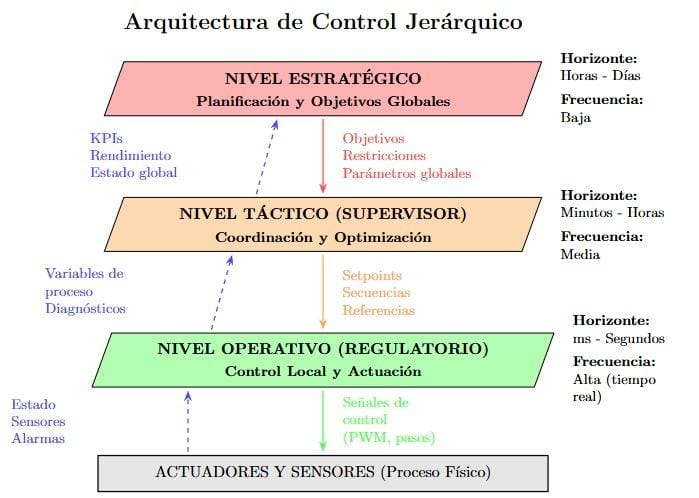
\includegraphics[width=0.8\textwidth]{img/jerarquia_control.jpg}
    \caption{Estructura piramidal de un sistema de control jerárquico mostrando los tres niveles, sus horizontes temporales y el flujo bidireccional de información (consignas descendentes y estado ascendente).}
    \label{fig:jerarquia_control}
\end{figure}
La adopción de una arquitectura de control jerárquica ofrece ventajas distintivas que justifican su uso en sistemas complejos:
\begin{itemize}
    \item Gestión de la Complejidad Dimensional: Permite abordar sistemas de gran escala al descomponer el problema de control multivariable en tareas más simples y manejables a nivel de subsistema.
    \item Confiabilidad y Robustez: Incrementa la resiliencia operativa, ya que el fallo localizado de un controlador en un nivel inferior solo afecta a un subsistema local, previniendo el colapso de la operación integral de la planta.
    \item Modularidad y Escalabilidad: Facilita la adición, modificación o reemplazo de subsistemas o unidades de control sin generar un impacto sistémico en el resto de la jerarquía.
    \item Eficiencia Operacional: Permite la aplicación de diferentes horizontes temporales y estrategias de control especializadas en cada nivel, optimizando tanto la estabilidad (Nivel 1) como la eficiencia global (Niveles 2 y 3).
\end{itemize}
Es crucial diferenciar el control jerárquico del control centralizado puro. Aunque el flujo de información y comando es vertical, el control jerárquico opera bajo un paradigma de control distribuido. El nivel superior impone únicamente las metas u objetivos macro, mientras que la implementación, la corrección de errores en corto plazo y la gestión de la dinámica local son responsabilidades inherentes y autónomas de los controladores ubicados en los niveles inferiores. Esta distribución de responsabilidades permite que cada nivel opere con la frecuencia y detalle apropiado a su función, evitando la saturación computacional característica de los sistemas centralizados.



\section{Fundamentos de visión artificial e inteligencia artificial}
\subsection{Procesamiento Digital de Imágenes}

El procesamiento digital de imágenes constituye el fundamento tecnológico de los sistemas de visión artificial en robótica agrícola. Esta disciplina integra conceptos de análisis matemático, álgebra lineal y teoría de señales para transformar datos visuales crudos en información estructurada y procesable por algoritmos de decisión.

\subsubsection{Representación Digital de Imágenes}

Una imagen digital se define matemáticamente como una función bidimensional discreta $f(x,y)$, donde las coordenadas espaciales $(x,y)$ representan posiciones en el plano de la imagen y el valor de la función indica la intensidad luminosa en cada punto. En el contexto de imágenes a color en formato RGB, esta representación se extiende a un espacio tridimensional:

\begin{equation}
\mathbf{I}(x,y) = \begin{bmatrix} R(x,y) \\ G(x,y) \\ B(x,y) \end{bmatrix} \in [0, 255]^3
\end{equation}

donde $R$, $G$ y $B$ representan los canales de color rojo, verde y azul respectivamente. Esta representación permite codificar aproximadamente 16.7 millones de colores distintos ($256^3$), cubriendo ampliamente el espectro visible necesario para aplicaciones de agricultura de precisión.

\begin{figure}[h]
\centering
\includegraphics[width=0.7\textwidth]{imagenes/representacion_imagen_rgb.png}
\caption{Representación de una imagen digital en el espacio RGB mostrando los tres canales de color}
\label{fig:representacion_rgb}
\end{figure}

La resolución espacial de una imagen determina la cantidad de información disponible para el análisis. Una imagen de dimensiones $M \times N$ píxeles contiene $M \cdot N$ elementos de información, cada uno representando el promedio de la radiancia incidente sobre el área del sensor correspondiente a ese píxel.

\subsubsection{Espacios de Color y Transformaciones}

El espacio de color RGB, aunque intuitivo y ampliamente utilizado en sistemas de captura, presenta limitaciones para ciertas tareas de procesamiento debido a su fuerte correlación entre canales y sensibilidad a variaciones de iluminación. Por esta razón, la conversión a espacios de color alternativos resulta fundamental en visión por computadora.

\textbf{Espacio HSV (Hue, Saturation, Value)}

El espacio HSV separa la información cromática (matiz y saturación) de la información de iluminación (valor), proporcionando robustez frente a cambios en las condiciones de luz. La transformación de RGB a HSV se define mediante:

\begin{equation}
V = \max(R, G, B)
\end{equation}

\begin{equation}
S = \begin{cases}
\frac{V - \min(R,G,B)}{V} & \text{si } V \neq 0 \\
0 & \text{si } V = 0
\end{cases}
\end{equation}

\begin{equation}
H = \begin{cases}
60° \cdot \frac{G-B}{V - \min(R,G,B)} & \text{si } V = R \\
60° \cdot \left(2 + \frac{B-R}{V - \min(R,G,B)}\right) & \text{si } V = G \\
60° \cdot \left(4 + \frac{R-G}{V - \min(R,G,B)}\right) & \text{si } V = B
\end{cases}
\end{equation}

\begin{figure}[h]
\centering
\includegraphics[width=0.8\textwidth]{imagenes/comparacion_rgb_hsv.png}
\caption{Comparación entre espacios de color RGB y HSV para una misma escena de cultivo}
\label{fig:comparacion_rgb_hsv}
\end{figure}

Esta descomposición resulta particularmente ventajosa para la detección de elementos basada en contraste, ya que el canal $V$ captura la intensidad luminosa independientemente del color, permitiendo operaciones de umbralización más robustas.

\textbf{Ventajas Operativas del Espacio HSV}

La separación de la información de brillo en el canal $V$ permite implementar algoritmos de detección invariantes a cambios de iluminación ambiental. En aplicaciones agrícolas donde las condiciones lumínicas varían significativamente durante el día, esta propiedad resulta crítica para mantener la consistencia operativa del sistema.

Matemáticamente, el canal $V$ satisface la propiedad de invariancia:

\begin{equation}
V(\alpha \cdot \mathbf{I}_{RGB}) = \alpha \cdot V(\mathbf{I}_{RGB}) \quad \forall \alpha > 0
\end{equation}

donde $\alpha$ representa un factor de escala de iluminación global. Esta linealidad permite compensar variaciones uniformes de brillo mediante ajustes simples de umbralización.

\subsubsection{Umbralización y Segmentación}

La umbralización constituye una técnica fundamental de segmentación que particiona una imagen en regiones de interés mediante la comparación de intensidades de píxeles contra valores de referencia. La umbralización binaria se define formalmente como:

\begin{equation}
g(x,y) = \begin{cases}
255 & \text{si } f(x,y) > T \\
0 & \text{si } f(x,y) \leq T
\end{cases}
\end{equation}

donde $T$ es el valor umbral y $g(x,y)$ es la imagen resultante.

\textbf{Umbralización Inversa}

En escenarios donde los elementos de interés presentan intensidades menores que el fondo, la umbralización inversa resulta más apropiada:

\begin{equation}
g(x,y) = \begin{cases}
255 & \text{si } f(x,y) < T \\
0 & \text{si } f(x,y) \geq T
\end{cases}
\end{equation}

Esta variante permite destacar regiones oscuras contra fondos claros, técnica ampliamente aplicada en la detección de marcadores de contraste en ambientes controlados.

\begin{figure}[h]
\centering
\includegraphics[width=0.7\textwidth]{imagenes/proceso_umbralizacion.png}
\caption{Proceso de umbralización binaria inversa para destacar elementos oscuros}
\label{fig:umbralizacion}
\end{figure}

\textbf{Selección Óptima del Umbral}

La determinación del valor umbral óptimo $T^*$ puede realizarse mediante análisis del histograma de intensidades. El método de Otsu minimiza la varianza intra-clase de los grupos resultantes:

\begin{equation}
T^* = \arg\min_T \left[\omega_0(T)\sigma_0^2(T) + \omega_1(T)\sigma_1^2(T)\right]
\end{equation}

donde $\omega_i$ y $\sigma_i^2$ representan el peso y varianza de cada clase. Alternativamente, puede emplearse conocimiento previo del entorno para establecer umbrales fijos que aprovechen características específicas del escenario operativo.

\subsubsection{Operaciones Morfológicas}

Las operaciones morfológicas manipulan la forma y estructura de objetos en imágenes binarias mediante la aplicación de elementos estructurantes. Estas operaciones se fundamentan en la teoría de conjuntos y permiten eliminar ruido, rellenar huecos y separar objetos conectados.

\textbf{Erosión}

La erosión reduce el tamaño de los objetos eliminando píxeles del perímetro:

\begin{equation}
(A \ominus B)(x,y) = \min_{(s,t) \in B} \{A(x+s, y+t)\}
\end{equation}

donde $A$ es la imagen binaria y $B$ es el elemento estructurante.

\textbf{Dilatación}

La dilatación expande los objetos añadiendo píxeles al perímetro:

\begin{equation}
(A \oplus B)(x,y) = \max_{(s,t) \in B} \{A(x+s, y+t)\}
\end{equation}

\textbf{Apertura y Cierre}

La apertura ($A \circ B = (A \ominus B) \oplus B$) elimina pequeños objetos y protuberancias, mientras el cierre ($A \bullet B = (A \oplus B) \ominus B$) rellena huecos pequeños y conecta componentes próximos. Estas operaciones compuestas resultan esenciales para el refinamiento de máscaras de segmentación en aplicaciones reales.

\begin{figure}[h]
\centering
\includegraphics[width=0.8\textwidth]{imagenes/operaciones_morfologicas.png}
\caption{Efecto de operaciones morfológicas sobre una imagen binaria}
\label{fig:operaciones_morfologicas}
\end{figure}

\subsubsection{Calibración y Transformación de Coordenadas}

La calibración establece la correspondencia entre coordenadas píxel en la imagen y coordenadas físicas en el espacio de trabajo. Esta transformación es fundamental para convertir mediciones visuales en comandos de movimiento precisos.

\textbf{Modelo de Transformación Lineal}

Para configuraciones donde la cámara observa perpendicular al plano de trabajo, la transformación píxel-a-métrica puede aproximarse mediante un modelo lineal:

\begin{equation}
\begin{bmatrix} x_{mm} \\ y_{mm} \end{bmatrix} = \begin{bmatrix} k_x & 0 \\ 0 & k_y \end{bmatrix} \begin{bmatrix} x_{px} \\ y_{px} \end{bmatrix} + \begin{bmatrix} t_x \\ t_y \end{bmatrix}
\end{equation}

donde $k_x, k_y$ son factores de escala (mm/píxel) y $t_x, t_y$ son desplazamientos de origen.

\textbf{Estimación por Mínimos Cuadrados}

Los parámetros de calibración se estiman mediante regresión lineal a partir de puntos de correspondencia conocidos:

\begin{equation}
\mathbf{K} = (\mathbf{X}^T\mathbf{X})^{-1}\mathbf{X}^T\mathbf{y}
\end{equation}

donde $\mathbf{X}$ contiene las coordenadas píxel de puntos de referencia, $\mathbf{y}$ sus coordenadas métricas medidas físicamente, y $\mathbf{K}$ el vector de parámetros de calibración. Este método minimiza el error cuadrático medio garantizando la solución óptima en el sentido de mínimos cuadrados.

\begin{figure}[h]
\centering
\includegraphics[width=0.7\textwidth]{imagenes/calibracion_camara.png}
\caption{Proceso de calibración mediante puntos de correspondencia conocidos}
\label{fig:calibracion}
\end{figure}

\textbf{Validación Estadística}

La precisión de la calibración se cuantifica mediante el error cuadrático medio (RMSE):

\begin{equation}
\text{RMSE} = \sqrt{\frac{1}{N}\sum_{i=1}^{N}(y_i - \hat{y}_i)^2}
\end{equation}

donde $\hat{y}_i$ son las predicciones del modelo. Valores de RMSE inferiores a 1mm resultan aceptables para aplicaciones de manipulación agrícola de precisión.
\subsection{Detección de Bordes y Líneas}

La detección de bordes identifica transiciones abruptas de intensidad en imágenes, correspondientes a límites entre objetos o regiones con propiedades visuales distintas. Estos bordes representan características estructurales fundamentales para reconocimiento de formas, medición dimensional y localización de elementos en el espacio. En aplicaciones de robótica agrícola, la detección de bordes permite identificar límites de tubos de cultivo, bordes de recipientes y estructuras de soporte sin depender exclusivamente del color o textura.

\subsubsection{Algoritmo de Canny}

El algoritmo de Canny, propuesto por John Canny en 1986, constituye uno de los métodos más efectivos y ampliamente utilizados para detección de bordes. El algoritmo se fundamenta en tres criterios de optimización: buena detección (baja tasa de falsos positivos y negativos), buena localización (bordes detectados próximos a los bordes reales), y respuesta única (un único punto de borde por cada borde real). La implementación sigue una secuencia de cinco etapas que progresivamente refinan la información hasta obtener bordes delgados y precisos.

\textbf{Reducción de Ruido mediante Filtrado Gaussiano}

La primera etapa aplica un filtro gaussiano bidimensional para suavizar la imagen y reducir ruido que podría generar bordes espurios. El kernel gaussiano se define como:

\begin{equation}
G(x,y) = \frac{1}{2\pi\sigma^2} e^{-\frac{x^2 + y^2}{2\sigma^2}}
\end{equation}

donde $\sigma$ controla el grado de suavizado. La imagen suavizada $I_s$ resulta de la convolución: $I_s = I \ast G$. Valores típicos de $\sigma$ entre 1.0 y 1.5 proporcionan balance entre reducción de ruido y preservación de bordes genuinos.

\textbf{Cálculo de Gradientes}

La segunda etapa calcula la magnitud y dirección del gradiente de intensidad en cada píxel. El gradiente se aproxima mediante operadores de Sobel:

\begin{equation}
G_x = \begin{bmatrix} -1 & 0 & 1 \\ -2 & 0 & 2 \\ -1 & 0 & 1 \end{bmatrix} \ast I_s, \quad G_y = \begin{bmatrix} 1 & 2 & 1 \\ 0 & 0 & 0 \\ -1 & -2 & -1 \end{bmatrix} \ast I_s
\end{equation}

La magnitud del gradiente $M = \sqrt{G_x^2 + G_y^2}$ indica la fuerza del borde, mientras que la dirección $\theta = \arctan(G_y/G_x)$ indica su orientación. Píxeles con alta magnitud de gradiente son candidatos a pertenecer a bordes.

\textbf{Supresión de No Máximos}

La tercera etapa adelgaza los bordes candidatos preservando únicamente píxeles que son máximos locales en la dirección del gradiente. Para cada píxel, se compara su magnitud de gradiente con la de sus dos vecinos en dirección perpendicular al borde. Si la magnitud del píxel no es mayor que ambos vecinos, se descarta. Esta operación garantiza que los bordes tengan grosor de un píxel, mejorando la localización.

\textbf{Doble Umbralización con Histéresis}

La cuarta etapa aplica dos umbrales para clasificar píxeles en tres categorías: bordes fuertes (magnitud > umbral alto), bordes débiles (magnitud entre umbral bajo y alto), y no bordes (magnitud < umbral bajo). Los bordes fuertes se aceptan inmediatamente. Los bordes débiles se aceptan únicamente si están conectados directa o indirectamente a un borde fuerte, mediante un algoritmo de seguimiento de contornos. Esta estrategia de histéresis reduce falsos positivos permitiendo que bordes genuinos con secciones débiles sean preservados, mientras que bordes débiles aislados (probablemente ruido) son rechazados.

La relación típica entre umbrales es $T_{alto} = 2 \cdot T_{bajo}$ o $3 \cdot T_{bajo}$, estableciéndose los valores absolutos experimentalmente según las características de la imagen. Para imágenes con buena iluminación, valores típicos como $T_{bajo} = 50$ y $T_{alto} = 150$ (en escala 0-255) suelen resultar efectivos.

\subsubsection{Transformada de Hough para Detección de Líneas}

Una vez detectados los bordes mediante Canny, la transformada de Hough permite identificar estructuras geométricas específicas como líneas rectas. El método se basa en representar cada punto de borde en un espacio de parámetros donde líneas rectas se manifiestan como puntos. Una línea recta en el espacio de imagen se parametriza mediante su distancia perpendicular al origen $\rho$ y el ángulo de la perpendicular $\theta$:

\begin{equation}
\rho = x \cos\theta + y \sin\theta
\end{equation}

Cada píxel de borde $(x_i, y_i)$ genera una curva sinusoidal en el espacio $(\theta, \rho)$ representando todas las líneas que podrían pasar por ese punto. Líneas colineales en el espacio de imagen producen curvas que se intersectan en un punto común del espacio de parámetros. Detectar estas intersecciones mediante acumulación de votos en un arreglo discretizado permite identificar las líneas presentes en la imagen.

La transformada de Hough probabilística optimiza este proceso muestreando aleatoriamente puntos de borde en lugar de procesarlos todos, reduciendo significativamente el costo computacional manteniendo precisión adecuada. El algoritmo retorna los puntos extremos de los segmentos de línea detectados, permitiendo filtrar líneas por longitud mínima y separación máxima entre segmentos.

\textbf{Parámetros de configuración:} Los parámetros clave de la transformada de Hough incluyen:
\begin{itemize}
\item \textbf{Resolución angular} ($\Delta\theta$): precisión en la discretización del ángulo
\item \textbf{Resolución de distancia} ($\Delta\rho$): precisión en la discretización de la distancia
\item \textbf{Umbral de votos}: número mínimo de puntos de borde que deben alinearse para considerar una línea válida
\item \textbf{Longitud mínima}: filtro para descartar segmentos de línea muy cortos
\item \textbf{Gap máximo}: distancia máxima permitida entre segmentos para considerarlos parte de la misma línea
\end{itemize}

La combinación de Canny y Hough constituye una herramienta fundamental para detectar estructuras rectilíneas en imágenes, aplicable a múltiples dominios como detección de carriles en vehículos autónomos, inspección de piezas manufacturadas, y localización de estructuras geométricas regulares.

\subsection{Detección y análisis de contornos}

La detección de contornos identifica las fronteras entre regiones con propiedades visuales distintas en imágenes binarias, proporcionando información estructural esencial para reconocimiento y clasificación de elementos. Un contorno se define matemáticamente como la secuencia ordenada de píxeles que forman el límite de una región conexa: $C = \{(x_i, y_i)\}_{i=1}^{n}$ donde $(x_i, y_i) \in \partial R$, siendo $\partial R$ la frontera topológica de la región $R$. Formalmente, un punto pertenece a la frontera si es parte de la región pero tiene al menos un vecino que no pertenece a ella. La conectividad del contorno se define por el vecindario considerado: 4-conectividad (vecinos arriba, abajo, izquierda, derecha) o 8-conectividad (incluyendo diagonales, generando contornos más suaves).

\subsubsection{Algoritmo de Suzuki-Abe}

El algoritmo de Suzuki-Abe, implementado en OpenCV mediante la función \texttt{findContours}, detecta simultáneamente contornos externos e internos organizándolos jerárquicamente. El algoritmo recorre la imagen binaria en orden raster (de izquierda a derecha, de arriba hacia abajo) y, al encontrar un píxel de objeto no visitado, inicia el rastreo del contorno siguiendo la frontera. La jerarquía resultante representa relaciones de anidamiento entre contornos mediante estructura de árbol.

\paragraph{\underline{Modos de recuperación de contornos:}}

Los modos de recuperación determinan qué contornos se extraen de la imagen:

\begin{itemize}[label=$\bullet$]
\item RETR\_EXTERNAL: extrae solo contornos externos de nivel superior, ignorando contornos internos (huecos dentro de objetos). Este modo es suficiente para aplicaciones donde interesan objetos individuales sin necesidad de analizar su estructura interna.

\item RETR\_LIST: extrae todos los contornos detectados (externos e internos) sin establecer relaciones jerárquicas entre ellos. Los contornos se almacenan en una lista plana.

\item RETR\_TREE: construye la jerarquía completa de contornos anidados, estableciendo relaciones padre-hijo entre contornos externos y sus contornos internos. Útil cuando se necesita analizar la estructura topológica completa.
\end{itemize}

\paragraph{\underline{Métodos de aproximación de contornos:}}

El parámetro de aproximación controla cómo se representan los puntos del contorno:

\begin{itemize}[label=$\bullet$]
\item CHAIN\_APPROX\_NONE: almacena todos los puntos del contorno sin compresión, preservando información geométrica completa. Por ejemplo, un segmento horizontal de 100 píxeles se representa con 100 puntos.

\item CHAIN\_APPROX\_SIMPLE: comprime segmentos horizontales, verticales y diagonales almacenando solo los puntos extremos, reduciendo significativamente el uso de memoria. El mismo segmento horizontal de 100 píxeles se representa con solo 2 puntos (inicio y fin).
\end{itemize}

\subsubsection{Descriptores geométricos}

Los descriptores cuantifican propiedades estructurales de contornos. El área encerrada se calcula mediante la fórmula del Shoelace:

\begin{equation}
A = \frac{1}{2}\left|\sum_{i=0}^{n-1}(x_i y_{i+1} - x_{i+1}y_i)\right|
\end{equation}

donde $(x_n, y_n) = (x_0, y_0)$ cierra el contorno. Este método tiene complejidad $\mathcal{O}(n)$ y proporciona área exacta del polígono. El perímetro se calcula sumando distancias euclidianas entre puntos consecutivos: $P = \sum_{i=0}^{n-1}\sqrt{(x_{i+1}-x_i)^2 + (y_{i+1}-y_i)^2}$.

El rectángulo delimitador (bounding box) es el rectángulo alineado a ejes que contiene completamente al contorno: $\text{BBox} = (x_{min}, y_{min}, w, h)$ donde $x_{min} = \min_i x_i$, $y_{min} = \min_i y_i$, $w = \max_i x_i - x_{min}$ y $h = \max_i y_i - y_{min}$. Este descriptor permite filtrar contornos por relación de aspecto o dimensiones absolutas.

El centroide representa el centro de masa geométrico del contorno:

\begin{equation}
\bar{x} = \frac{1}{6A}\sum_{i=0}^{n-1}(x_i + x_{i+1})(x_i y_{i+1} - x_{i+1}y_i), \quad \bar{y} = \frac{1}{6A}\sum_{i=0}^{n-1}(y_i + y_{i+1})(x_i y_{i+1} - x_{i+1}y_i)
\end{equation}

Este punto resulta fundamental para cálculos de desviación espacial en sistemas de corrección de posicionamiento visual.

\subsubsection{Filtrado y selección de contornos}

Las imágenes binarias reales contienen múltiples contornos, muchos correspondientes a ruido o elementos irrelevantes. El filtrado elimina contornos no deseados según criterios del problema. El filtrado por área establece límites: $A_{min} \leq A_{contorno} \leq A_{max}$. Los umbrales se definen según el tamaño esperado de objetos; por ejemplo, $A_{min} = 0.01 \cdot A_{imagen}$ filtra ruido puntual mientras que $A_{max} = 0.6 \cdot A_{imagen}$ elimina regiones que abarcan casi toda la imagen.

El filtrado por posición descarta contornos que tocan bordes de la imagen (generalmente incompletos) o que no contienen el punto central (bajo asunción de objeto centrado en campo de visión). El filtrado por forma emplea relación de aspecto $AR = w/h$ del bounding box para discriminar orientaciones: valores $AR > 2$ indican objetos horizontales, $AR < 0.5$ objetos verticales, y valores intermedios formas aproximadamente cuadradas.

Cuando múltiples contornos cumplen filtros básicos, se implementa un sistema de scoring que pondera múltiples criterios para seleccionar el mejor candidato. Un score típico combina área normalizada, distancia del centroide al centro de imagen, y métricas de calidad de forma:

\begin{equation}
S_{total} = w_1 \cdot S_{área} + w_2 \cdot S_{posición} + w_3 \cdot S_{forma}
\end{equation}

donde los pesos $w_i$ (con $\sum w_i = 1$) reflejan importancia relativa de cada aspecto según el problema. Cada componente $S_i$ se normaliza típicamente al rango $[0,1]$ para que contribuyan de manera equilibrada al score total. El contorno con mayor score es seleccionado como el objeto de interés.

\subsubsection{Análisis de regiones parciales}

En aplicaciones donde la geometría varía entre zonas del objeto, analizar regiones específicas del contorno proporciona descriptores más robustos que el contorno completo. Este enfoque particiona el contorno en segmentos y analiza cada uno por separado.

\paragraph{\underline{Ejemplo de partición por altura:}} \textit{Para objetos con base regular pero parte superior irregular, se puede analizar únicamente una región inferior del contorno:}

\begin{equation}
R_{base} = \{(x,y) \in C : y \geq y_{max} - \alpha h\}
\end{equation}

donde $C$ es el contorno completo, $h$ es la altura del bounding box, y $\alpha \in (0,1)$ define la fracción de altura a analizar (típicamente $\alpha = 0.1$ para el 10\% inferior). Sobre esta región se pueden calcular descriptores específicos como:

\begin{itemize}[label=$\bullet$]
\item Ancho efectivo de la base: $w_{base} = \max_{(x,y) \in R_{base}} x - \min_{(x,y) \in R_{base}} x + 1$

\item Ocupación de la base: fracción de píxeles presentes respecto al rectángulo delimitador de la región, calculada como:
\begin{equation}
\text{Ocupación} = \frac{|R_{base}|}{w_{base} \cdot (\alpha h)}
\end{equation}
\end{itemize}

Bases sólidas rectangulares presentan ocupación superior a 0.8, mientras que formas irregulares o fragmentadas tienen menor ocupación, permitiendo discriminación efectiva entre diferentes tipos de objetos.

Este enfoque de análisis por regiones resulta particularmente valioso cuando las condiciones de captura introducen variabilidad en ciertas zonas del objeto pero otras zonas mantienen geometría consistente y predecible.

\subsection{Clasificación Basada en Análisis Morfológico}

La clasificación morfológica de objetos utiliza características geométricas y estadísticas extraídas de contornos e imágenes para asignar categorías a elementos detectados. A diferencia de métodos de aprendizaje profundo, este enfoque se fundamenta en reglas explícitas derivadas del conocimiento del dominio y análisis estadístico de datos representativos.

\subsubsection{Fundamentos de Clasificación por Umbrales}

El método más directo de clasificación morfológica establece límites de decisión basados en valores de descriptores geométricos. Para un descriptor $d$ y un conjunto de clases $\mathcal{C} = \{c_1, c_2, ..., c_n\}$, la regla de clasificación se define como:

\begin{equation}
\text{Clase}(x) = c_i \quad \text{si} \quad t_{i-1} < d(x) \leq t_i
\end{equation}

donde $t_0, t_1, ..., t_n$ son umbrales que particionan el espacio de características.

\textbf{Clasificación por Área}

Para objetos que se diferencian principalmente por tamaño, el área en píxeles constituye un descriptor efectivo:

\begin{equation}
\text{Clase}(C) = \begin{cases}
\text{Pequeño} & \text{si } A < t_1 \\
\text{Mediano} & \text{si } t_1 \leq A < t_2 \\
\text{Grande} & \text{si } A \geq t_2
\end{cases}
\end{equation}

La robustez del método depende de la separabilidad entre clases. La distancia entre centroides de clases adyacentes debe ser significativa respecto a la dispersión intra-clase.

\subsubsection{Análisis Estadístico para Determinación de Umbrales}

La selección óptima de umbrales requiere análisis estadístico de una base de datos representativa de cada clase.

\textbf{Parámetros Estadísticos por Clase}

Para cada clase $c_i$, se calculan la media y desviación estándar del descriptor de interés:

\begin{equation}
\mu_i = \frac{1}{N_i}\sum_{j=1}^{N_i} d_j
\end{equation}

\begin{equation}
\sigma_i = \sqrt{\frac{1}{N_i-1}\sum_{j=1}^{N_i}(d_j - \mu_i)^2}
\end{equation}

donde $N_i$ es el número de muestras de la clase $i$, $\mu_i$ es la media y $\sigma_i$ la desviación estándar del descriptor $d$.

\textbf{Determinación de Umbrales mediante Análisis de Distribuciones}

Asumiendo distribuciones normales para cada clase:

\begin{equation}
P(d|c_i) = \frac{1}{\sigma_i\sqrt{2\pi}} \exp\left(-\frac{(d-\mu_i)^2}{2\sigma_i^2}\right)
\end{equation}

Para distribuciones con igual varianza ($\sigma_i = \sigma_{i+1} = \sigma$), el umbral óptimo entre clases consecutivas es:

\begin{equation}
t_i^* = \frac{\mu_i + \mu_{i+1}}{2}
\end{equation}

Este umbral minimiza la probabilidad de error cuando las clases tienen igual probabilidad a priori y varianzas similares.

\subsubsection{Clasificación Multi-Criterio con Ratios de Color}

Cuando un único descriptor geométrico no proporciona separabilidad suficiente, se emplean múltiples características simultáneamente. En el contexto de agricultura de precisión, los ratios de color resultan particularmente efectivos.

\textbf{Espacio de Características de Color}

Dado un contorno, se calculan ratios que cuantifican la proporción de diferentes componentes cromáticos:

\begin{equation}
r_{verde} = \frac{N_{píxeles\_verdes}}{N_{píxeles\_totales}}
\end{equation}

\begin{equation}
r_{negro} = \frac{N_{píxeles\_negros}}{N_{píxeles\_totales}}
\end{equation}

donde $N_{píxeles\_totales} = N_{píxeles\_verdes} + N_{píxeles\_negros} + N_{píxeles\_otros}$.

Cada objeto se representa como un vector en el espacio de características:

\begin{equation}
\mathbf{x} = [r_{verde}, r_{negro}, I_{media}]^T
\end{equation}

donde $I_{media}$ es la intensidad promedio de píxeles internos.

\textbf{Prototipos de Clase}

Para cada clase $c_i$, se define un prototipo mediante las medias de los descriptores:

\begin{equation}
\boldsymbol{\mu}_i = [\mu_{verde,i}, \mu_{negro,i}, \mu_{intensidad,i}]^T
\end{equation}

\textbf{Desviaciones Estándar por Clase}

Las variaciones dentro de cada clase se cuantifican mediante:

\begin{equation}
\boldsymbol{\sigma}_i = [\sigma_{verde,i}, \sigma_{negro,i}, \sigma_{intensidad,i}]^T
\end{equation}

\subsubsection{Distancia Euclidiana Normalizada}

Para clasificar un objeto nuevo, se calcula su distancia a cada prototipo de clase. La normalización por desviación estándar garantiza que descriptores con diferentes rangos contribuyan equitativamente.

\textbf{Distancia Normalizada}

La distancia de un objeto $\mathbf{x}$ al prototipo de la clase $c_i$ se define como:

\begin{equation}
D_i(\mathbf{x}) = \sqrt{\sum_{k=1}^{m} \left(\frac{x_k - \mu_{k,i}}{\sigma_{k,i} + \epsilon}\right)^2}
\end{equation}

donde:
\begin{itemize}
\item $m$ es el número de descriptores (ej. 3 para verde, negro, intensidad)
\item $x_k$ es el valor del descriptor $k$ para el objeto
\item $\mu_{k,i}$ es la media del descriptor $k$ para la clase $i$
\item $\sigma_{k,i}$ es la desviación estándar del descriptor $k$ para la clase $i$
\item $\epsilon$ es un término pequeño (ej. $10^{-6}$) para evitar división por cero
\end{itemize}

\textbf{Regla de Clasificación por Mínima Distancia}

El objeto se asigna a la clase con menor distancia normalizada:

\begin{equation}
\text{Clase}(\mathbf{x}) = \arg\min_{i} D_i(\mathbf{x})
\end{equation}

Este criterio implementa un clasificador de vecino más cercano en el espacio normalizado.

\textbf{Cálculo de Confianza}

La confianza de la clasificación se deriva de las distancias relativas:

\begin{equation}
\text{Confianza} = 1 - \frac{D_{min}}{D_{max} + D_{min}}
\end{equation}

donde $D_{min}$ es la distancia a la clase predicha y $D_{max}$ la distancia a la clase más lejana. Valores cercanos a 1 indican alta confianza; valores cercanos a 0.5 sugieren ambigüedad.

Para mejorar robustez, la confianza se limita:

\begin{equation}
\text{Confianza}_{final} = \max(0.3, \min(1.0, \text{Confianza}))
\end{equation}

garantizando un rango $[0.3, 1.0]$.

\subsubsection{Ejemplo: Clasificación de Cultivos}

Para un sistema de clasificación de tubos de cultivo con tres clases:

\begin{itemize}
\item \textbf{LECHUGAS}: Alto ratio verde ($r_{verde} > 0.40$)
\item \textbf{PLANTINES}: Ratio verde moderado, alto ratio negro
\item \textbf{VASOS} (vacíos): Muy bajo ratio verde, alto ratio negro
\end{itemize}

\textbf{Prototipos Estimados}

A partir de un dataset de entrenamiento:

\begin{equation}
\boldsymbol{\mu}_{LECHUGAS} = [0.65, 0.35, 120]^T, \quad \boldsymbol{\sigma}_{LECHUGAS} = [0.15, 0.15, 30]^T
\end{equation}

\begin{equation}
\boldsymbol{\mu}_{PLANTINES} = [0.45, 0.55, 90]^T, \quad \boldsymbol{\sigma}_{PLANTINES} = [0.15, 0.15, 25]^T
\end{equation}

\begin{equation}
\boldsymbol{\mu}_{VASOS} = [0.05, 0.95, 50]^T, \quad \boldsymbol{\sigma}_{VASOS} = [0.10, 0.10, 20]^T
\end{equation}

\textbf{Clasificación de Muestra}

Dado un objeto con descriptores $\mathbf{x} = [0.60, 0.40, 115]^T$:

\begin{equation}
D_{LECHUGAS} = \sqrt{\left(\frac{0.60-0.65}{0.15}\right)^2 + \left(\frac{0.40-0.35}{0.15}\right)^2 + \left(\frac{115-120}{30}\right)^2} = 0.47
\end{equation}

\begin{equation}
D_{PLANTINES} = \sqrt{\left(\frac{0.60-0.45}{0.15}\right)^2 + \left(\frac{0.40-0.55}{0.15}\right)^2 + \left(\frac{115-90}{25}\right)^2} = 1.52
\end{equation}

\begin{equation}
D_{VASOS} = \sqrt{\left(\frac{0.60-0.05}{0.10}\right)^2 + \left(\frac{0.40-0.95}{0.10}\right)^2 + \left(\frac{115-50}{20}\right)^2} = 8.56
\end{equation}

La clase predicha es LECHUGAS ($D_{min} = 0.47$) con confianza:

\begin{equation}
\text{Confianza} = 1 - \frac{0.47}{8.56 + 0.47} = 0.95
\end{equation}

\subsubsection{Análisis de Separabilidad de Clases}

La efectividad de un conjunto de descriptores para clasificación se cuantifica mediante métricas de separabilidad.

\textbf{Criterio de Fisher}

Mide la razón entre varianza inter-clase e intra-clase para un descriptor $d$:

\begin{equation}
J_F = \frac{(\mu_1 - \mu_2)^2}{\sigma_1^2 + \sigma_2^2}
\end{equation}

Valores altos de $J_F$ indican buena separabilidad. Para múltiples clases:

\begin{equation}
J_F = \frac{\sum_{i=1}^{C} N_i(\mu_i - \mu_{global})^2}{\sum_{i=1}^{C} N_i \sigma_i^2}
\end{equation}

donde $\mu_{global}$ es la media global ponderada.

\textbf{Índice de Solapamiento}

Para distribuciones gaussianas, el solapamiento entre clases $i$ y $j$ se aproxima:

\begin{equation}
\text{Overlap}_{i,j} \approx 2\Phi\left(-\frac{|\mu_i - \mu_j|}{2\sqrt{\sigma_i^2 + \sigma_j^2}}\right)
\end{equation}

donde $\Phi$ es la función de distribución acumulada normal estándar. Valores cercanos a 0 indican separación perfecta; valores cercanos a 1 indican fuerte solapamiento.

\subsubsection{Validación Estadística del Clasificador}

\textbf{Exactitud Estimada}

La exactitud de un clasificador se define como:

\begin{equation}
\text{Exactitud} = \frac{N_{correctas}}{N_{total}}
\end{equation}

donde $N_{correctas}$ es el número de clasificaciones correctas y $N_{total}$ el tamaño del conjunto de prueba.

\textbf{Intervalo de Confianza}

El intervalo de confianza al 95\% para la exactitud es:

\begin{equation}
\text{IC}_{95\%} = \hat{p} \pm 1.96\sqrt{\frac{\hat{p}(1-\hat{p})}{n}}
\end{equation}

donde $\hat{p}$ es la exactitud observada y $n$ el tamaño de la muestra de prueba.

\textbf{Tamaño de Muestra Requerido}

Para estimar la exactitud con error máximo $E$ y nivel de confianza del 95\%:

\begin{equation}
n_{min} = \left(\frac{1.96 \cdot \sqrt{\hat{p}(1-\hat{p})}}{E}\right)^2
\end{equation}

Por ejemplo, para $E = 0.05$ (error de 5\%) y $\hat{p} = 0.9$:

\begin{equation}
n_{min} = \left(\frac{1.96 \cdot \sqrt{0.9 \cdot 0.1}}{0.05}\right)^2 \approx 139
\end{equation}

Se requieren al menos 139 muestras de prueba.

\subsubsection{Robustez y Generalización}

\textbf{Validación Cruzada k-fold}

Para evaluar la generalización del clasificador, se emplea validación cruzada:

\begin{enumerate}
\item Dividir dataset en $k$ particiones de igual tamaño (típicamente $k=5$ o $k=10$)
\item Para $i = 1$ a $k$:
   \begin{itemize}
   \item Usar partición $i$ como conjunto de prueba
   \item Usar restantes $k-1$ particiones para calcular prototipos ($\boldsymbol{\mu}_i$, $\boldsymbol{\sigma}_i$)
   \item Evaluar exactitud en partición $i$
   \end{itemize}
\item Calcular exactitud promedio
\end{enumerate}

La exactitud estimada por validación cruzada es:

\begin{equation}
\text{Exactitud}_{CV} = \frac{1}{k}\sum_{i=1}^{k} \text{Exactitud}_i
\end{equation}

Esta métrica proporciona una estimación más realista del desempeño en datos nuevos que la evaluación en un único conjunto de prueba.

\textbf{Sensibilidad a Variaciones}

La robustez ante ruido se evalúa añadiendo perturbaciones controladas a los descriptores:

\begin{equation}
d_{ruidoso} = d_{verdadero} + \mathcal{N}(0, \sigma_{ruido}^2)
\end{equation}

donde $\mathcal{N}(0, \sigma_{ruido}^2)$ es ruido gaussiano con desviación estándar $\sigma_{ruido}$.

Un clasificador robusto mantiene exactitud alta incluso con $\sigma_{ruido}$ moderado. La degradación de desempeño se cuantifica como:

\begin{equation}
\Delta\text{Exactitud} = \text{Exactitud}_{limpio} - \text{Exactitud}_{ruidoso}
\end{equation}

Degradaciones $\Delta\text{Exactitud} < 0.1$ (10\%) indican robustez aceptable.

\subsubsection{Ventajas y Limitaciones del Enfoque Morfológico}

\textbf{Ventajas:}
\begin{itemize}
\item \textbf{Interpretabilidad}: Reglas de decisión explícitas y comprensibles basadas en características físicas medibles
\item \textbf{Eficiencia computacional}: Cálculos geométricos y estadísticos simples, ejecución en tiempo real en hardware embebido
\item \textbf{Pocos datos requeridos}: Decenas a cientos de muestras por clase, vs. miles requeridos por aprendizaje profundo
\item \textbf{Control explícito}: Ajuste directo de umbrales y pesos según requerimientos operativos
\item \textbf{Depuración sencilla}: Fallas identificables mediante inspección de valores de descriptores
\item \textbf{Sin dependencias externas}: No requiere frameworks de deep learning ni GPUs
\end{itemize}

\textbf{Limitaciones:}
\begin{itemize}
\item \textbf{Diseño manual de características}: Requiere conocimiento experto del dominio para identificar descriptores relevantes
\item \textbf{Limitada a características medibles}: No captura patrones visuales complejos o texturas sutiles
\item \textbf{Sensibilidad a condiciones}: Variaciones significativas de iluminación o perspectiva pueden afectar descriptores
\item \textbf{Separabilidad lineal}: Dificultad con clases no linealmente separables en el espacio de características
\item \textbf{Escalabilidad a muchas clases}: Desempeño puede degradar con >10 clases
\end{itemize}

\textbf{Aplicabilidad en Agricultura de Precisión}

El enfoque morfológico resulta particularmente adecuado para clasificación de cultivos cuando:
\begin{enumerate}
\item Existe diferenciación clara por tamaño, forma o color (plantines vs. plantas maduras vs. tubos vacíos)
\item El entorno es controlado (cultivo hidropónico con iluminación artificial)
\item Se requiere operación en hardware con recursos limitados (Raspberry Pi, microcontroladores)
\item La interpretabilidad del sistema es crítica para validación agronómica
\item El número de clases es limitado (2-5 categorías)
\item Se dispone de conocimiento experto para diseñar descriptores relevantes
\end{enumerate}

La combinación con análisis estadístico robusto permite alcanzar exactitudes >90\% en escenarios donde las características geométricas y cromáticas son discriminativas, sin la complejidad y requisitos computacionales de métodos de aprendizaje profundo.

\subsubsection{Técnicas Adicionales para Robustez}

\textbf{Normalización de Descriptores}

Antes de calcular distancias, normalizar descriptores al rango $[0,1]$ evita que características con rangos grandes dominen:

\begin{equation}
d_{norm} = \frac{d - d_{min}}{d_{max} - d_{min}}
\end{equation}

donde $d_{min}$ y $d_{max}$ son los valores mínimo y máximo observados en el dataset de entrenamiento.

\textbf{Umbral de Rechazo}

Para evitar clasificaciones erróneas en objetos anómalos, se establece un umbral máximo de distancia:

\begin{equation}
\text{Clase}(\mathbf{x}) = \begin{cases}
\arg\min_{i} D_i(\mathbf{x}) & \text{si } D_{min} < T_{rechazo} \\
\text{DESCONOCIDO} & \text{si } D_{min} \geq T_{rechazo}
\end{cases}
\end{equation}

Objetos con $D_{min} \geq T_{rechazo}$ son rechazados como no pertenecientes a ninguna clase conocida.

\textbf{Actualización de Prototipos}

En aplicaciones donde las características de las clases evolucionan (ej. crecimiento de plantas), los prototipos pueden actualizarse incrementalmente:

\begin{equation}
\boldsymbol{\mu}_i^{nuevo} = \alpha \cdot \boldsymbol{\mu}_i^{viejo} + (1-\alpha) \cdot \mathbf{x}_{nuevo}
\end{equation}

donde $\alpha \in [0.9, 0.99]$ controla la tasa de adaptación.

\subsection{Métricas de evaluación}

La evaluación cuantitativa del desempeño de sistemas de clasificación y calibración requiere métricas que capturen la calidad predictiva del modelo. Resulta fundamental seleccionar métricas apropiadas que reflejen los objetivos operativos del sistema.

\subsubsection{Métricas para clasificación}

La matriz de confusión constituye la representación fundamental del desempeño de un clasificador, tabulando predicciones versus etiquetas verdaderas. Para un problema de $C$ clases, la matriz de confusión $\mathbf{M} \in \mathbb{R}^{C \times C}$ tiene elementos:

\begin{equation}
M_{ij} = \sum_{k=1}^{N} \mathbb{1}[y_k = i \land \hat{y}_k = j]
\end{equation}

donde $y_k$ es la clase verdadera de la muestra $k$, $\hat{y}_k$ es la clase predicha, y $\mathbb{1}[\cdot]$ es la función indicadora. Los elementos diagonales representan clasificaciones correctas, mientras que los elementos fuera de la diagonal representan errores.

\begin{table}[h]
\centering
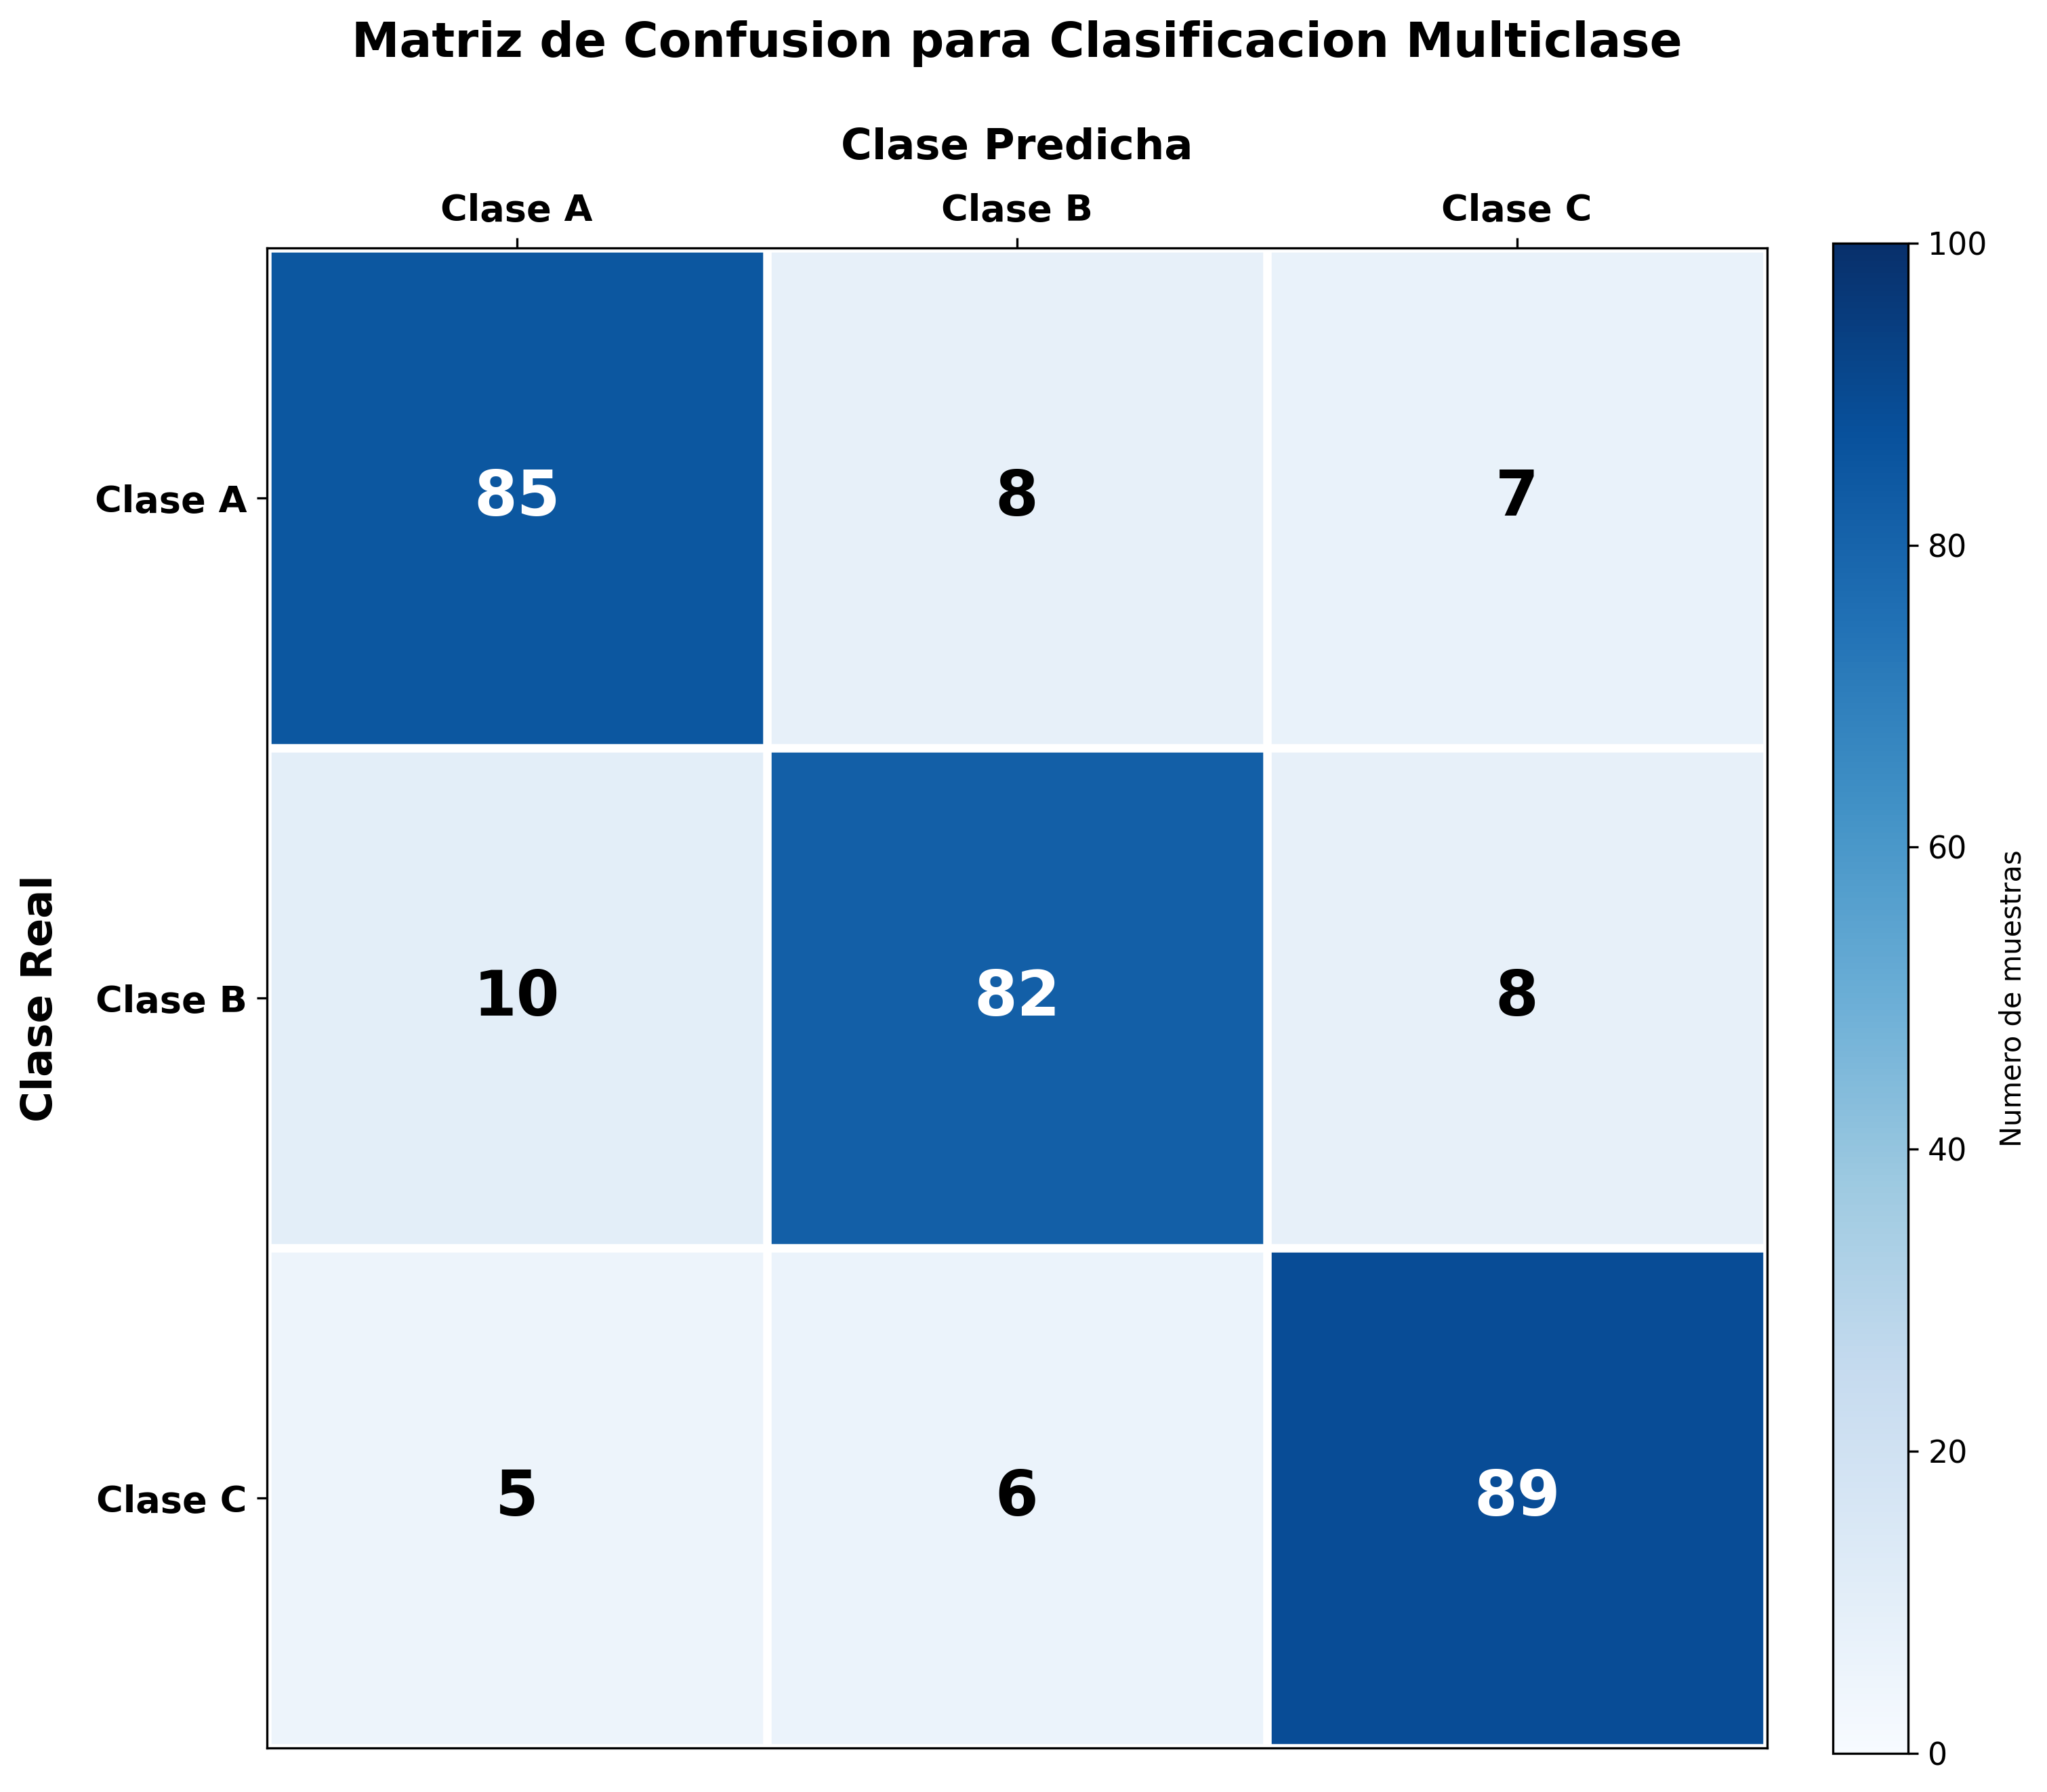
\includegraphics[width=0.65\textwidth]{imagenes/matriz_confusion_ejemplo.png}
\caption{\textit{Matriz de confusión para clasificación multiclase}}
\label{fig:matriz_confusion}
\end{table}

La precisión cuantifica la proporción de predicciones positivas correctas: $\text{Precision} = \text{TP}/(\text{TP} + \text{FP})$. La exhaustividad mide la proporción de casos positivos reales identificados: $\text{Recall} = \text{TP}/(\text{TP} + \text{FN})$. Existe un compromiso inherente entre precisión y recall: aumentar el umbral de decisión incrementa la precisión pero reduce el recall, y viceversa.

\subsubsection{Métricas para calibración espacial}

En sistemas de calibración píxel-milímetro, se emplean métricas de error continuo. El error cuadrático medio (RMSE) cuantifica la magnitud típica de los errores:

\begin{equation}
\text{RMSE} = \sqrt{\frac{1}{N}\sum_{i=1}^{N}(y_i - \hat{y}_i)^2}
\end{equation}

El coeficiente de determinación $R^2$ mide la proporción de varianza explicada por el modelo:

\begin{equation}
R^2 = 1 - \frac{\sum_{i=1}^{N}(y_i - \hat{y}_i)^2}{\sum_{i=1}^{N}(y_i - \bar{y})^2}
\end{equation}

Valores de $R^2$ cercanos a 1 indican excelente ajuste lineal del modelo. Para aplicaciones de agricultura de precisión, se requiere bajo RMSE (típicamente <2mm) y alto $R^2$ (>0.99) para garantizar precisión en el posicionamiento.


\section{Estructuras cartesianas y robots serie}
\subsection{Estructuras Cartesianas}

Las estructuras cartesianas, también conocidas como sistemas de coordenadas cartesianas o robots cartesianos, son mecanismos de posicionamiento que permiten el movimiento controlado en un espacio tridimensional mediante el desplazamiento lineal a lo largo de tres ejes perpendiculares entre sí: X, Y y Z. Estos sistemas son ampliamente utilizados en aplicaciones industriales y de fabricación digital, como impresoras 3D, máquinas CNC (Control Numérico Computarizado), plotters y sistemas de pick-and-place.

\subsubsection{Principio de Funcionamiento}

El principio fundamental de las estructuras cartesianas se basa en la descomposición del movimiento espacial en tres componentes lineales independientes. Cada eje está constituido por:

\begin{itemize}
    \item \textbf{Guías lineales:} Elementos mecánicos que definen la trayectoria del movimiento y minimizan la fricción. Pueden ser barras cilíndricas pulidas, rieles con rodamientos lineales o perfiles de aluminio con rodamientos en V.
    
    \item \textbf{Sistema de transmisión:} Mecanismo encargado de convertir el movimiento rotacional del motor en desplazamiento lineal. Los más comunes incluyen tornillos de bolas, tornillos trapezoidales, correas dentadas y cremalleras.
    
    \item \textbf{Actuadores:} Generalmente motores paso a paso (stepper) o servomotores, que proporcionan el movimiento controlado y preciso necesario para el posicionamiento.
    
    \item \textbf{Estructura de soporte:} Marco rígido que mantiene la alineación de todos los componentes y soporta las cargas operativas.
\end{itemize}

\subsubsection{Configuraciones Comunes}

Existen diversas configuraciones de estructuras cartesianas, cada una con ventajas específicas según la aplicación:

\paragraph{Configuración de Pórtico (Gantry):}En esta configuración, utilizada frecuentemente en máquinas CNC y algunas impresoras 3D, el eje X se monta sobre dos columnas verticales (eje Y) que se desplazan simultáneamente. Esta disposición proporciona mayor rigidez y capacidad de carga, siendo ideal para áreas de trabajo amplias.

\paragraph{Configuración CoreXY:}Sistema en el que los ejes X e Y comparten dos motores mediante un sistema de correas cruzadas. Esta configuración reduce la masa móvil en el eje vertical y permite velocidades de desplazamiento superiores, siendo popular en impresoras 3D de alto rendimiento.

\paragraph{Configuración Cartesiana Pura:} Cada eje se mueve de forma completamente independiente, con el efector final (cabezal de impresión, husillo, etc.) montado sucesivamente sobre cada eje. Es la configuración más simple conceptualmente y facilita el mantenimiento.

\subsubsection{Ventajas de las Estructuras Cartesianas}

Las estructuras cartesianas presentan múltiples ventajas que explican su amplia adopción:

\begin{itemize}
    \item \textbf{Precisión y repetibilidad:} El movimiento lineal directo minimiza errores acumulativos y permite alcanzar tolerancias del orden de micrones.
    
    \item \textbf{Simplicidad de control:} La cinemática directa simplifica significativamente los algoritmos de control, ya que existe una correspondencia uno a uno entre las coordenadas del espacio de trabajo y las posiciones de los actuadores.
    
    \item \textbf{Volumen de trabajo optimizado:} El espacio útil de trabajo se aproxima al volumen total de la máquina, maximizando la eficiencia espacial.
    
    \item \textbf{Escalabilidad:} Es relativamente sencillo modificar las dimensiones de trabajo extendiendo o reduciendo la longitud de los ejes.
    
    \item \textbf{Rigidez estructural:} Las guías lineales y la disposición ortogonal proporcionan alta rigidez, crucial para aplicaciones de mecanizado.
\end{itemize}

\subsection{Aplicaciones}

Las estructuras cartesianas encuentran aplicación en diversos campos:

\begin{itemize}
    \item \textbf{Manufactura aditiva:} Impresoras 3D FDM, SLA y SLS
    \item \textbf{Mecanizado:} Fresadoras CNC, routers, máquinas de corte por plasma
    \item \textbf{Ensamblaje:} Robots pick-and-place, dispensadores de adhesivos
    \item \textbf{Medición:} Máquinas de medición por coordenadas (CMM)
    \item \textbf{Biomedicina:} Bioimpresorasa y sistemas de dispensación de fluidos
\end{itemize}

\subsection{Robots Serie}

Los robots serie, también denominados robots en cadena cinemática abierta, son aquellos en los que los eslabones están conectados secuencialmente mediante juntas, formando una cadena cinemática desde la base hasta el efector final. Cada eslabón está conectado al anterior mediante una única junta, que puede ser rotacional (R) o prismática (P).

\subsubsection{Grados de Libertad}

El número de grados de libertad de un robot serie corresponde al número de juntas activas en la cadena cinemática. Para manipulación completa en el espacio tridimensional (posición y orientación arbitrarias), se requieren 6 GDL. Un robot con $n$ juntas tiene $n$ grados de libertad:

\begin{itemize}
    \item Si $n < 6$: El robot tiene movilidad limitada y no puede alcanzar poses arbitrarias
    \item Si $n = 6$: El robot puede alcanzar cualquier posición y orientación dentro de su espacio de trabajo
    \item Si $n > 6$: El robot es redundante, ofreciendo múltiples configuraciones para una misma pose del efector final
\end{itemize}

\subsubsection{Espacio de Trabajo}

El espacio de trabajo de un robot serie es generalmente más complejo que el de un robot cartesiano y depende fuertemente de la configuración específica de juntas. Típicamente, el espacio de trabajo tiene forma de cáscara esférica, toroidal, o cilíndrica, con regiones inaccesibles y posibles singularidades.

Para un robot con $n$ juntas, donde cada junta $i$ tiene límites $q_i \in [q_{i,\min}, q_{i,\max}]$, el espacio de trabajo alcanzable se define como:

\begin{equation}
\mathcal{W} = \{\mathbf{p} \in \mathbb{R}^3 \mid \mathbf{p} = f(\mathbf{q}), \, \mathbf{q} \in \mathcal{Q}\}
\end{equation}

donde $f(\mathbf{q})$ es la función de cinemática directa y $\mathcal{Q}$ es el espacio de configuraciones:

\begin{equation}
\mathcal{Q} = \{\mathbf{q} \in \mathbb{R}^n \mid q_{i,\min} \leq q_i \leq q_{i,\max}, \, i = 1, \ldots, n\}
\end{equation}

El espacio de trabajo se subdivide en:

\begin{itemize}
    \item \textbf{Espacio alcanzable}: Conjunto de puntos que el efector final puede alcanzar desde al menos una orientación
    \item \textbf{Espacio diestro}: Conjunto de puntos alcanzables desde múltiples orientaciones
    \item \textbf{Singularidades}: Configuraciones donde se pierde un grado de libertad instantáneo
\end{itemize}

\subsubsection{Cinemática}

\paragraph{Cinemática Directa:} 

La cinemática directa de robots serie se resuelve mediante la convención de Denavit-Hartenberg (DH), que establece un sistema de coordenadas en cada junta y describe la transformación entre eslabones consecutivos mediante cuatro parámetros: $a_i$ (longitud del eslabón), $\alpha_i$ (ángulo de torsión), $d_i$ (offset), y $\theta_i$ (ángulo de junta).

La matriz de transformación homogénea entre los eslabones $i-1$ e $i$ se expresa como:

\begin{equation}
{}^{i-1}T_i = 
\begin{bmatrix}
\cos\theta_i & -\sin\theta_i\cos\alpha_i & \sin\theta_i\sin\alpha_i & a_i\cos\theta_i \\
\sin\theta_i & \cos\theta_i\cos\alpha_i & -\cos\theta_i\sin\alpha_i & a_i\sin\theta_i \\
0 & \sin\alpha_i & \cos\alpha_i & d_i \\
0 & 0 & 0 & 1
\end{bmatrix}
\end{equation}

La pose del efector final respecto a la base se obtiene mediante la composición de transformaciones:

\begin{equation}
{}^0T_n = {}^0T_1 \cdot {}^1T_2 \cdot \ldots \cdot {}^{n-1}T_n
\end{equation}

\paragraph{Cinemática Inversa:}

El problema de cinemática inversa consiste en determinar las variables de junta $\mathbf{q}$ que posicionan el efector final en una pose deseada. A diferencia de los robots cartesianos, este problema puede tener:

\begin{itemize}
    \item Múltiples soluciones (hasta 16 para robots de 6 GDL)
    \item Una única solución
    \item Ninguna solución (pose fuera del espacio de trabajo)
\end{itemize}

Los métodos de solución incluyen técnicas geométricas, algebraicas, y numéricas como el método de Newton-Raphson o el Jacobiano inverso.

\subsubsection{Jacobiano y Singularidades}

El Jacobiano del robot relaciona las velocidades de las juntas con las velocidades del efector final:

\begin{equation}
\dot{\mathbf{x}} = J(\mathbf{q}) \dot{\mathbf{q}}
\end{equation}

donde $\dot{\mathbf{x}} \in \mathbb{R}^6$ representa las velocidades lineales y angulares del efector final, y $\dot{\mathbf{q}} \in \mathbb{R}^n$ son las velocidades de las juntas.

Las singularidades ocurren cuando $\det(J(\mathbf{q})) = 0$, resultando en pérdida de movilidad o control. Se clasifican en:

\begin{itemize}
    \item \textbf{Singularidades de frontera}: En los límites del espacio de trabajo
    \item \textbf{Singularidades internas}: Dentro del espacio de trabajo, donde dos o más ejes se alinean
\end{itemize}

%\subsubsection{Planificación de Trayectorias}

%La planificación de trayectorias en robots ser<ie es más compleja debido a la naturaleza no lineal de su cinemática. Las estrategias comunes incluyen:

%\paragraph{Trayectorias en el espacio de juntas:}

%Interpolación directa entre configuraciones de junta inicial $\mathbf{q}_0$ y final $\mathbf{q}_f$:

%\begin{equation}
%\mathbf{q}(t) = \mathbf{q}_0 + s(t)(\mathbf{q}_f - \mathbf{q}_0)
%\end{equation}

%donde $s(t)$ es una función de sincronización temporal, típicamente polinomial de grado 3 o 5 para garantizar continuidad en velocidad y aceleración.

%\paragraph{Trayectorias en el espacio cartesiano:}

%Requieren cinemática inversa en cada punto de la trayectoria. Para una trayectoria lineal en el espacio cartesiano:

%\begin{equation}
%\mathbf{x}(t) = \mathbf{x}_0 + s(t)(\mathbf{x}_f - \mathbf{x}_0)
%\end{equation}

%seguida de la resolución del problema inverso: $\mathbf{q}(t) = f^{-1}(\mathbf{x}(t))$.

%\paragraph{Evitación de singularidades:}

%La planificación debe considerar las singularidades del robot, modificando trayectorias o añadiendo restricciones para evitar configuraciones problemáticas donde el control se vuelve inestable.

\subsubsection{Dinámica}

La dinámica de robots serie se describe mediante las ecuaciones de Euler-Lagrange, resultando en el modelo dinámico:

\begin{equation}
M(\mathbf{q})\ddot{\mathbf{q}} + C(\mathbf{q}, \dot{\mathbf{q}})\dot{\mathbf{q}} + G(\mathbf{q}) = \boldsymbol{\tau}
\end{equation}

donde $M(\mathbf{q})$ es la matriz de inercia, $C(\mathbf{q}, \dot{\mathbf{q}})$ representa las fuerzas de Coriolis y centrífugas, $G(\mathbf{q})$ es el vector de torques gravitacionales, y $\boldsymbol{\tau}$ son los torques aplicados en las juntas.

\subsubsection{Ventajas y Aplicaciones}

Las ventajas de los robots serie incluyen:

\begin{itemize}
    \item Gran versatilidad y flexibilidad de movimiento
    \item Espacio de trabajo amplio relativo a su tamaño
    \item Capacidad de alcanzar posiciones en espacios confinados
    \item Variedad de configuraciones para diferentes aplicaciones
\end{itemize}

Se utilizan extensivamente en soldadura robotizada, pintura, ensamblaje automotriz, cirugía asistida, manipulación de piezas, paletizado, y aplicaciones colaborativas con humanos.
\subsubsection{Consideraciones Prácticas sobre el Control Dinámico}

En la práctica industrial y de fabricación digital contemporánea, el cálculo explícito del modelo dinámico completo del robot mediante las ecuaciones de Euler-Lagrange raramente se realiza a nivel del controlador del robot. Esto se debe a que los actuadores modernos incorporan sus propios sistemas de control que gestionan la dinámica local de forma autónoma.

\paragraph{Servomotores y Drivers Inteligentes}

Los servomotores vienen equipados con drivers que implementan lazos de control en cascada: lazo de corriente que controla el par motor instantáneo con frecuencias de actualización, lazo de velocidad que regula la velocidad angular mediante un controlador PID típicamente a 1-5 kHz y lazo de posición que gestiona el posicionamiento angular con actualizaciones de 100-1000 Hz.

Estos drivers manejan internamente: compensación de inercia del rotor, limitación de corriente y par, perfiles trpaezoidales de aceleración/desaceleración, detección de pérdida de pasos o sobrecarga

El controlador del robot simplemente envía consignas de posición, velocidad o par sin necesidad de calcular los torques requeridos.

\paragraph{Motores Paso a Paso con Control de Lazo Abierto}

El driver genera las secuencias de pulsos para los devanados del motor, envía sol pulsos de paso y dirección y la dinámica item El controlador envía únicamente pulsos de paso y dirección y la dinámica se gestiona limitando aceleraciones máximas en el firmware

Incluso aquí, el modelo dinámico se reduce a parámetros empíricos de aceleración máxima configurados en el firmware, sin cálculos formales de las ecuaciones de movimiento.

\subsubsection{Implicaciones para el Diseño de Controladores}

Esta arquitectura de control distribuido tiene consecuencias importantes.

\paragraph{Ventajas:}

\begin{itemize}
    \item \textbf{Simplificación del software de control}: El programador del robot trabaja en el espacio de juntas o cartesiano sin preocuparse por la física subyacente.
    
    \item \textbf{Modularidad}: Se pueden intercambiar actuadores de diferentes fabricantes manteniendo la misma lógica de control superior.
    
    \item \textbf{Robustez}: Los lazos internos de los drivers responden mucho más rápido que cualquier controlador de alto nivel podría.
    
    \item \textbf{Menor carga computacional}: El procesador principal del robot (Arduino, Raspberry Pi, controlador industrial) solo ejecuta cinemática y planificación de trayectorias.
\end{itemize}

\paragraph{Limitaciones:}

\begin{itemize}
    \item \textbf{Desacoplamiento de ejes}: Cada motor actúa independientemente sin considerar las interacciones dinámicas con otros eslabones. Esto puede causar:
    \begin{itemize}
        \item Vibraciones residuales en movimientos rápidos
        \item Mayor consumo energético
        \item Limitaciones en la precisión a altas velocidades
    \end{itemize}
    
    \item \textbf{Sobre-dimensionamiento}: Sin modelo dinámico, los motores suelen seleccionarse con márgenes de seguridad conservadores.
    
    \item \textbf{Dificultad en movimientos coordinados complejos}: Tareas como manipulación de objetos flexibles o control de fuerza son más desafiantes.
\end{itemize}

La mayoría de aplicaciones de robótica industrial, estructuras cartesianas e impresoras 3D, \textbf{el control dinámico está efectivamente ``resuelto'' por los fabricantes de actuadores}. El ingeniero de aplicación se concentra en:

\begin{itemize}
    \item Cinemática (directa e inversa)
    \item Planificación de trayectorias
    \item Configuración adecuada de parámetros PID en los drivers
    \item Selección apropiada de actuadores según carga y dinámica esperada
\end{itemize}

Solo en aplicaciones que requieren máximo rendimiento, eficiencia energética óptima, o capacidades avanzadas como control de fuerza, se justifica implementar control basado en modelo dinámico completo.


\section{Sistemas de transmisión mecánica}
% Transmisión

\subsection{Sistemas de Transmisión}

El sistema mecánico del cosechador emplea dos tipos principales de transmisión para convertir el movimiento rotacional de los motores en movimiento lineal y rotacional según los requerimientos de cada eje:

\subsubsection{Transmisión por Correa Dentada y Poleas}

\paragraph{Principio de funcionamiento}
La transmisión por correa dentada consiste en una correa flexible con dientes en su superficie interna que engranan con poleas dentadas solidarias a los ejes motor y conducido. Este sistema permite transmitir potencia y movimiento entre ejes paralelos con alta eficiencia y sin deslizamiento.

\paragraph{Ventajas del sistema}
\begin{itemize}
    \item \textbf{Transmisión sincrónica:} Los dientes de la correa engranan positivamente con las poleas, eliminando el deslizamiento y garantizando una relación de transmisión exacta
    \item \textbf{Alta eficiencia:} Eficiencia típica del 96-98\%, superior a sistemas de correas trapezoidales
    \item \textbf{Bajo mantenimiento:} No requiere lubricación y presenta mínimo desgaste en condiciones normales de operación
    \item \textbf{Operación silenciosa:} El engrane de los dientes minimiza vibraciones y ruido
    \item \textbf{Flexibilidad de diseño:} Permite implementar diferentes relaciones de transmisión mediante la selección de poleas de distintos diámetros
    \item \textbf{Bajo momento de inercia:} La correa es liviana, lo que facilita arranques y paradas rápidas
\end{itemize}

\paragraph{Componentes del sistema}
\begin{enumerate}
    \item \textbf{Polea motriz:} Montada en el eje del motor, transmite el movimiento rotacional a la correa. Su diámetro primitivo determina la velocidad de salida junto con el diámetro de la polea conducida.

    \item \textbf{Polea conducida:} Montada en el eje a accionar, recibe el movimiento desde la correa. La relación de diámetros entre ambas poleas define la relación de transmisión:
    \begin{equation}
        i = \frac{D_2}{D_1} = \frac{n_1}{n_2} = \frac{z_2}{z_1}
    \end{equation}
    donde $D$ son los diámetros primitivos, $n$ las velocidades angulares y $z$ el número de dientes de las poleas motriz (1) y conducida (2).

    \item \textbf{Correa dentada:} Elemento flexible con perfil dentado estandarizado. Los perfiles más comunes son:
    \begin{itemize}
        \item GT2 (2\,mm de paso): Utilizado en aplicaciones de precisión como impresoras 3D y CNC
        \item GT3 (3\,mm de paso): Mayor capacidad de carga que GT2
        \item HTD (High Torque Drive): Para aplicaciones de alta potencia
        \item T-series y AT-series: Perfiles trapezoidales para uso general
    \end{itemize}
\end{enumerate}

\paragraph{Cálculo de la relación de transmisión}
Para un sistema con polea motriz de $z_1$ dientes y polea conducida de $z_2$ dientes:
\begin{equation}
    n_2 = n_1 \cdot \frac{z_1}{z_2}
\end{equation}

La longitud de correa requerida para una distancia entre centros $C$ se calcula como:
\begin{equation}
    L = 2C + \frac{\pi(D_1 + D_2)}{2} + \frac{(D_2 - D_1)^2}{4C}
\end{equation}

\paragraph{Tensado de la correa}
El tensado adecuado es crítico para el funcionamiento correcto:
\begin{itemize}
    \item \textbf{Tensión insuficiente:} Produce saltos de dientes y pérdida de sincronismo
    \item \textbf{Tensión excesiva:} Incrementa el desgaste de la correa y aumenta la carga sobre los rodamientos
\end{itemize}

La tensión estática recomendada se calcula como:
\begin{equation}
    T_s = \frac{1.5 \cdot P}{v} + m \cdot v^2
\end{equation}
donde $P$ es la potencia transmitida, $v$ la velocidad lineal de la correa y $m$ la masa por unidad de longitud.

\paragraph{Aplicación en el sistema}
En el movimiento horizontal del cosechador, la transmisión por correa dentada se emplea para:
\begin{itemize}
    \item Transferir el movimiento del motor al husillo de movimiento
    \item Permitir la ubicación del motor en una posición que optimice el balance de masas
    \item Reducir o amplificar la velocidad según los requerimientos cinemáticos
    \item Minimizar las vibraciones transmitidas entre motor y carro móvil
\end{itemize}

\subsubsection{Transmisión por Varilla Roscada (Husillo)}

\paragraph{Principio de funcionamiento}
La transmisión por varilla roscada, también conocida como sistema tornillo-tuerca, convierte el movimiento rotacional en movimiento lineal mediante el principio de la rosca helicoidal. Cuando la varilla roscada gira, la tuerca acoplada a ella se desplaza linealmente a lo largo del eje de la varilla.

\paragraph{Tipos de roscas}
\begin{enumerate}
    \item \textbf{Rosca trapezoidal (ACME o TR):}
    \begin{itemize}
        \item Perfil trapezoidal con ángulo de flanco de 30° (ACME) o 15° (TR métrica)
        \item Alta resistencia al desgaste
        \item Buena capacidad de carga axial
        \item Eficiencia típica: 30-50\%
        \item Auto-frenante en la mayoría de configuraciones (ángulo de hélice bajo)
        \item Aplicación: Movimiento vertical del sistema
    \end{itemize}

    \item \textbf{Husillo de bolas:}
    \begin{itemize}
        \item Recirculación de bolas entre la rosca y la tuerca
        \item Mínima fricción (contacto rodante vs. deslizante)
        \item Eficiencia típica: 90-95\%
        \item No es auto-frenante
        \item Mayor precisión y vida útil
        \item Costo significativamente mayor
    \end{itemize}
\end{enumerate}

\paragraph{Relación de transmisión}
El desplazamiento lineal por revolución está determinado por el paso de la rosca:
\begin{equation}
    \Delta x = n \cdot p
\end{equation}
donde $n$ es el número de revoluciones y $p$ es el paso de la rosca.

Para rosca de múltiples entradas:
\begin{equation}
    p_{\text{efectivo}} = N_e \cdot p_{\text{nominal}}
\end{equation}
donde $N_e$ es el número de entradas.

\paragraph{Análisis de fuerzas y torque}
El torque necesario para mover una carga $F$ mediante una varilla roscada incluye dos componentes:

\textbf{1. Torque de subida:}
\begin{equation}
T_{\text{subida}} = \frac{F \cdot d_m}{2} \cdot k_R + \frac{F \cdot \mu_c \cdot d_c}{2}
\label{eq:torque_subida}
\end{equation}

\textbf{2. Torque de bajada:}
\begin{equation}
T_{\text{bajada}} = \frac{F \cdot d_m}{2} \cdot k_L + \frac{F \cdot \mu_c \cdot d_c}{2}
\label{eq:torque_bajada}
\end{equation}

El torque total resulta:
\begin{equation}
    T_{\text{total}} = T_{\text{subida}} + T_{\text{bajada}} 
    \label{eq:torque_total_varilla}
\end{equation}

donde:
\begin{itemize}
    \item F: Carga a desplazar.
    \item $d_m$: diámetro medio de la rosca
    \item $d_c$: diámetro medio del collarín
    \item $\mu_c$:coeficiente de fricción del collarín
    \item $k_R$:  factor de rosca para subida, incluye efecto de cuña y fricción
    \item $k_L$: factor de rosca para bajada
\end{itemize}

\paragraph{Eficiencia del sistema}
La eficiencia de la transmisión se define como:
\begin{equation}
    \eta = \frac{\tan(\alpha)}{\tan(\alpha + \phi)}
\end{equation}

Para roscas trapezoidales típicas con $\mu \approx 0.1-0.2$ (lubricadas), la eficiencia varía entre 30\% y 50\%.

\paragraph{Condición de auto-frenado}
Un sistema de tornillo-tuerca es auto-frenante (la carga no puede hacer girar la varilla) cuando:
\begin{equation}
    \alpha < \phi \quad \Rightarrow \quad \tan(\alpha) < \mu
\end{equation}

Esto es deseable en aplicaciones verticales donde se requiere mantener la posición sin energía en el motor.

\paragraph{Carga crítica y pandeo}
Para varillas largas trabajando a compresión, debe verificarse la carga crítica de Euler:
\begin{equation}
    P_{\text{cr}} = \frac{\pi^2 \cdot E \cdot I}{(K \cdot L)^2}
\end{equation}

donde $E$ es el módulo de Young, $I$ el momento de inercia de la sección, $L$ la longitud y $K$ el factor de longitud efectiva según las condiciones de apoyo.

\paragraph{Vida útil y desgaste}
El desgaste en roscas trapezoidales depende de:
\begin{itemize}
    \item Presión de contacto entre rosca y tuerca
    \item Velocidad de deslizamiento
    \item Calidad de la lubricación
    \item Material de la tuerca (bronce, polímeros, acero)
\end{itemize}

La vida útil se estima mediante:
\begin{equation}
    L_{10} = \left(\frac{C_a}{F}\right)^3 \cdot 10^6 \quad \text{[mm de recorrido]}
\end{equation}
donde $C_a$ es la capacidad de carga dinámica de la tuerca y $F$ la carga aplicada.

\paragraph{Aplicación en el sistema}
En el movimiento vertical del cosechador, la transmisión por varilla trapezoidal TR16$\times$4 se emplea debido a:
\begin{itemize}
    \item \textbf{Auto-frenado:} Mantiene la posición vertical sin consumo energético continuo
    \item \textbf{Simplicidad:} No requiere sistemas de bloqueo adicionales
    \item \textbf{Costo:} Significativamente menor que husillos de bolas
    \item \textbf{Robustez:} Tolera mejor condiciones adversas (polvo, humedad)
    \item \textbf{Precisión suficiente:} Con 200 pasos/mm se logra la resolución requerida para el posicionamiento
\end{itemize}

El sistema trabaja principalmente a tracción (varilla fija superior, carga colgante) lo que minimiza problemas de pandeo, aunque se verifica la estabilidad estructural para garantizar seguridad ante cualquier eventualidad.


\section{Control de motores paso a paso}

Los motores paso a paso (stepper motors) son actuadores electromecánicos que convierten pulsos eléctricos digitales en movimientos angulares discretos y precisos. A diferencia de los motores de corriente continua convencionales, los motores paso a paso se mueven en incrementos angulares fijos llamados pasos, lo que permite un control de posición en lazo abierto sin necesidad de retroalimentación encoders, aunque estos pueden añadirse para aplicaciones críticas.

\subsubsection{Principio de funcionamiento}

El funcionamiento de un motor paso a paso se basa en la conmutación secuencial de las corrientes en sus bobinas estatóricas, generando campos magnéticos que interactúan con el rotor magnetizado o dentado. Cada pulso de control provoca un movimiento angular discreto del rotor hacia la siguiente posición de equilibrio magnético estable.

El ángulo de paso $\alpha$ define la resolución angular del motor y se expresa como:

\begin{equation}
\alpha = \frac{360^\circ}{N_p}
\end{equation}

donde $N_p$ es el número de pasos por revolución. Los valores típicos de pasos por revolución son 200 ($1.8^\circ$ por paso), 400 ($0.9^\circ$ por paso), aunque mediante técnicas de microstepping se pueden alcanzar resoluciones mucho mayores.

\subsection{Modos de excitación y control}

El modo de excitación define cómo se energizan las bobinas del motor, afectando directamente el torque, la precisión, el consumo de energía y la suavidad del movimiento.

\subsubsection{Excitación de Paso Completo (Full Step)}

\paragraph{Modo de una fase:}

Solo una bobina se energiza a la vez. La secuencia de activación para un motor bipolar de dos fases es:

\begin{table}[ht]
\centering
\begin{tabular}{|c|c|c|}
\hline
\textbf{Paso} & \textbf{Fase A} & \textbf{Fase B} \\
\hline
1 & +I & 0 \\
2 & 0 & +I \\
3 & -I & 0 \\
4 & 0 & -I \\
\hline
\end{tabular}
\caption{Secuencia de excitación Wave Drive}
\end{table}

Características:
\begin{itemize}
    \item Menor consumo de corriente (50\% respecto a dos fases)
    \item Torque reducido (aproximadamente 70\% del torque nominal)
    \item Mayor resonancia a ciertas velocidades
\end{itemize}

\paragraph{Modo de dos fases (Full step):}

Dos bobinas se energizan simultáneamente. La secuencia de activación es:

\begin{table}[ht]
\centering
\begin{tabular}{|c|c|c|}
\hline
\textbf{Paso} & \textbf{Fase A} & \textbf{Fase B} \\
\hline
1 & +I & +I \\
2 & -I & +I \\
3 & -I & -I \\
4 & +I & -I \\
\hline
\end{tabular}
\caption{Secuencia de excitación Full Step}
\end{table}

Características:
\begin{itemize}
    \item Máximo torque disponible (100\% del torque nominal)
    \item Mayor consumo de corriente y generación de calor
    \item Mejor estabilidad posicional
\end{itemize}

\subsubsection{Excitación de medio paso (Half step)}

Alterna entre la energización de una y dos fases, duplicando la resolución del motor. La secuencia combina los modos anteriores:

\begin{table}[ht]
\centering
\begin{tabular}{|c|c|c|}
\hline
\textbf{Paso} & \textbf{Fase A} & \textbf{Fase B} \\
\hline
1 & +I & 0 \\
2 & +I & +I \\
3 & 0 & +I \\
4 & -I & +I \\
5 & -I & 0 \\
6 & -I & -I \\
7 & 0 & -I \\
8 & +I & -I \\
\hline
\end{tabular}
\caption{Secuencia de excitación Half Step}
\end{table}

Para un motor de 200 pasos/rev ($1.8^\circ$), el half stepping proporciona 400 pasos/rev ($0.9^\circ$).

Características:
\begin{itemize}
    \item Resolución duplicada respecto al full step
    \item Torque variable entre pasos (70-100\%)
    \item Mayor suavidad de movimiento
    \item Reducción de resonancia
\end{itemize}

\subsubsection{Microstepping}

El microstepping es una técnica avanzada que subdivide cada paso completo en múltiples micropasos mediante la modulación sinusoidal de las corrientes en las bobinas. Las corrientes en las fases A y B se controlan según:

\begin{equation}
\begin{aligned}
I_A(\theta) &= I_{\max} \cos(\theta) \\
I_B(\theta) &= I_{\max} \sin(\theta)
\end{aligned}
\end{equation}

donde $\theta$ es el ángulo eléctrico deseado e $I_{\max}$ es la corriente máxima nominal.

Para $M$ micropasos por paso completo, el ángulo de micropaso es:

\begin{equation}
\alpha_{\mu} = \frac{\alpha}{M} = \frac{360^\circ}{N_p \cdot M}
\end{equation}

Niveles comunes de microstepping incluyen 1/4, 1/8, 1/16, 1/32, hasta 1/256 pasos.

\paragraph{Ventajas del microstepping:}

\begin{itemize}
    \item Resolución extremadamente alta (hasta 51,200 pasos/rev con 1/256)
    \item Movimiento muy suave y silencioso
    \item Eliminación virtual de resonancia a bajas velocidades
    \item Mejor precisión en posicionamiento fino
\end{itemize}

\paragraph{Limitaciones del microstepping:}

\begin{itemize}
    \item La resolución teórica no garantiza precisión posicional debido a no linealidades
    \item Reducción de torque en micropasos intermedios
    \item Mayor complejidad del driver y procesamiento requerido
    \item Sensibilidad a fricción y errores mecánicos
\end{itemize}

\subsection{Características de desempeño}

\subsubsection{Curvas de torque}

El desempeño de un motor paso a paso se caracteriza principalmente mediante dos curvas de torque:

\paragraph{Torque de retención (Holding torque):}

Es el torque máximo que el motor puede ejercer cuando está energizado pero estacionario. Representa la capacidad de mantener la posición contra cargas externas. Se expresa en N·m o kg·cm y es un parámetro fundamental de selección.

\paragraph{Torque dinámico (Pull-out Torque):}

Es el torque máximo disponible durante el movimiento a una velocidad dada. Esta curva es crítica para determinar si el motor puede acelerar y mantener una carga específica a la velocidad deseada.

La relación entre torque y velocidad se aproxima por:

\begin{equation}
T(\omega) = T_0 \sqrt{1 - \left(\frac{\omega}{\omega_{\max}}\right)^2}
\end{equation}

donde $T_0$ es el torque a velocidad cero (aproximadamente el holding torque), $\omega$ es la velocidad angular, y $\omega_{\max}$ es la velocidad máxima sin carga.

\subsection{Drivers y electrónica de control}

\subsubsection{Tipos de drivers}

\paragraph{Driver unipolar:}

Diseñado para motores unipolares (generalmente con 5 o 6 cables). Utiliza transistores simples para conmutar las corrientes. Ventajas: simplicidad y bajo costo. Desventajas: menor eficiencia y torque (aproximadamente 70\% del equivalente bipolar).

\paragraph{Driver bipolar:}

Para motores bipolares (4 cables). Requiere puentes H para invertir la polaridad de las corrientes. Mayor complejidad pero mejor desempeño. Topologías comunes:

\begin{itemize}
    \item \textbf{L/R Drive}: Control de voltaje simple, genera calor excesivo
    \item \textbf{Chopper Drive}: Modulación PWM de corriente, mayor eficiencia
    \item \textbf{Bipolar con control de corriente}: Regulación precisa mediante sensado de corriente
\end{itemize}

\subsubsection{Interfaces de control}

\paragraph{Step/Direction:}

La interfaz más común. Dos señales digitales:
\begin{itemize}
    \item \textbf{STEP}: Cada pulso produce un paso (o micropaso)
    \item \textbf{DIRECTION}: Define el sentido de rotación (HIGH/LOW)
\end{itemize}

Adicionalmente pueden incluirse señales ENABLE (habilitar motor) y FAULT (indicación de error).

\paragraph{Control por pulsos y sentido:}

Variante donde pulsos en dos líneas diferentes determinan dirección:
\begin{itemize}
    \item Pulsos en CW: Rotación horaria
    \item Pulsos en CCW: Rotación antihoraria
\end{itemize}

\paragraph{Comunicación serial/bus:}

Drivers avanzados incorporan interfaces RS-485, CANbus, o EtherCAT para configuración de parámetros, diagnóstico y control centralizado en sistemas multi-eje.

\subsection{Generación de perfiles de movimiento}

\subsubsection{Perfil trapezoidal}

El perfil de velocidad trapezoidal es el más utilizado por su simplicidad y efectividad. Consta de tres fases:

\begin{enumerate}
    \item \textbf{Aceleración}: Incremento lineal de velocidad desde reposo hasta velocidad objetivo
    \item \textbf{Velocidad constante}: Mantenimiento de la velocidad máxima
    \item \textbf{Deceleración}: Reducción lineal hasta detenerse
\end{enumerate}

Para un desplazamiento angular $\theta_{total}$, con aceleración $\alpha$ y velocidad máxima $\omega_{max}$:

Tiempo de aceleración:
\begin{equation}
t_{acc} = \frac{\omega_{max}}{\alpha}
\end{equation}

Ángulo durante aceleración:
\begin{equation}
\theta_{acc} = \frac{1}{2}\alpha t_{acc}^2 = \frac{\omega_{max}^2}{2\alpha}
\end{equation}

Si el movimiento permite alcanzar $\omega_{max}$:
\begin{equation}
\theta_{cruise} = \theta_{total} - 2\theta_{acc}
\end{equation}

Tiempo total:
\begin{equation}
t_{total} = 2t_{acc} + \frac{\theta_{cruise}}{\omega_{max}}
\end{equation}

Para movimientos cortos donde no se alcanza $\omega_{max}$, la velocidad pico es:
\begin{equation}
\omega_{peak} = \sqrt{\alpha \cdot \theta_{total}}
\end{equation}

\subsection{Análisis de fallos comunes}
\begin{itemize}

    \item{Pérdida de pasos}

\paragraph{Causas:}Torque requerido excede torque disponible, aceleración excesiva, resonancia mecánica, voltaje de alimentación insuficiente a alta velocidad o carga mecánica variable o impactos.

\paragraph{Soluciones:}Aumentar corriente del motor (si térmicamente posible), reducir aceleración máxima, implementar microstepping, incrementar voltaje de alimentación, seleccionar motor de mayor torque o añadir reducción mecánica.

    \item{Resonancia y vibración}

\paragraph{Mitigación:}Cambiar a microstepping (mínimo 1/8), evitar velocidades resonantes en trayectorias, implementar perfiles S-curve, añadir masa o amortiguadores mecánicos, utilizar drivers con anti-resonance features

    \item {Sobrecalentamiento}

\paragraph{Límites térmicos:}La temperatura superficial del motor no debe exceder:
\begin{equation}
T_{surface} < T_{ambient} + \Delta T_{rated}
\end{equation}

Típicamente, $\Delta T_{rated} = 80^\circ$C sobre ambiente.

\paragraph{Soluciones:}Reducir corriente en configuración del driver (sacrificando torque), implementar reducción de corriente en reposo, mejorar ventilación o añadir disipadores, reducir ciclo de trabajo, seleccionar motor de mayor frame size con mejor capacidad térmica.
\end{itemize}

%Los motores paso a paso continúan siendo una solución óptima para aplicaciones que requieren posicionamiento preciso, control digital directo, y operación confiable sin sistemas de retroalimentación complejos. La selección adecuada mediante un proceso sistemático, combinada con configuración apropiada del driver y técnicas de control avanzadas, garantiza un desempeño óptimo y vida útil prolongada del sistema.
%% Modos Operacion


%% Drivers Electronica


\section{Microcontroladores y comunicación}
En sistemas de control jerárquico, es común utilizar distintas plataformas de hardware según las capacidades de procesamiento requeridas en cada nivel. Los microcontroladores se especializan en tareas de control en tiempo real y manejo directo de periféricos, mientras que los microprocesadores ofrecen mayor capacidad de cómputo para algoritmos complejos y gestión de alto nivel.

\subsubsection{Arduino Mega 2560}

El Arduino Mega 2560 es una plataforma de desarrollo basada en el microcontrolador ATmega2560 de 8 bits. Sus características principales incluyen:

\begin{itemize}
    \item \textbf{Procesador:} ATmega2560 con arquitectura AVR a 16 MHz
    \item \textbf{Memoria:} 256 KB de memoria Flash, 8 KB de SRAM y 4 KB de EEPROM
    \item \textbf{Entradas/Salidas:} 54 pines digitales (15 con PWM) y 16 entradas analógicas
    \item \textbf{Interfaces de comunicación:} 4 puertos UART, I²C y SPI
    \item \textbf{Tensión de operación:} 5V
\end{itemize}

Esta plataforma es ideal para tareas de control en tiempo real, generación de señales PWM, lectura de sensores y control directo de actuadores. Su arquitectura de 8 bits y ejecución determinística la hacen especialmente adecuada para el nivel regulatorio de un sistema de control jerárquico.

\subsubsection{Raspberry Pi 5}

La Raspberry Pi 5 es un computador de placa única (SBC) basado en un procesador ARM de 64 bits. Sus características principales son:

\begin{itemize}
    \item \textbf{Procesador:} Broadcom BCM2712 Quad-core ARM Cortex-A76 a 2.4 GHz
    \item \textbf{Memoria RAM:} 4 u 8 GB LPDDR4X
    \item \textbf{GPU:} VideoCore VII con soporte para gráficos OpenGL ES 3.1
    \item \textbf{Conectividad:} Gigabit Ethernet, Wi-Fi 802.11ac, Bluetooth 5.0
    \item \textbf{Interfaces:} GPIO de 40 pines, UART, I²C, SPI, USB 3.0, HDMI
    \item \textbf{Sistema operativo:} Linux (Raspberry Pi OS, Ubuntu, etc.)
\end{itemize}

La Raspberry Pi es ideal para tareas computacionalmente intensivas como procesamiento de imágenes, inteligencia artificial, gestión de bases de datos y supervisión de sistemas complejos. Su capacidad para ejecutar sistemas operativos completos permite el desarrollo de aplicaciones de alto nivel en lenguajes como Python o C++.

\subsubsection{Protocolo de comunicación UART}

UART (Universal Asynchronous Receiver-Transmitter) es un protocolo de comunicación serial asíncrono ampliamente utilizado para la interconexión entre microcontroladores y computadores. Sus características principales son:

\begin{itemize}
    \item \textbf{Comunicación punto a punto:} Conexión directa entre dos dispositivos mediante dos líneas: TX (transmisión) y RX (recepción)
    \item \textbf{Asíncrono:} No requiere señal de reloj compartida; los dispositivos deben configurarse con la misma velocidad de transmisión (baud rate)
    \item \textbf{Configuración común:} 8 bits de datos, 1 bit de parada, sin paridad (8N1)
    \item \textbf{Velocidades típicas:} 9600, 19200, 38400, 57600, 115200 baudios
    \item \textbf{Niveles lógicos:} 0V para nivel bajo y 3.3V o 5V para nivel alto (según el dispositivo)
\end{itemize}

\textbf{Estructura de una trama UART:}

Una trama UART típica consiste en:
\begin{enumerate}
    \item \textbf{Bit de inicio (Start bit):} Marca el comienzo de la transmisión (nivel bajo)
    \item \textbf{Bits de datos:} Generalmente 8 bits que contienen la información
    \item \textbf{Bit de paridad (opcional):} Para detección de errores
    \item \textbf{Bits de parada (Stop bits):} Uno o dos bits que marcan el fin de la trama (nivel alto)
\end{enumerate}

%%%%%%%%%%%%%%%%%%%%%%%%%%%%%%%%%%%%%%%%%%%%%%%%%%%%%%%%%%%%%%%
% CAPÍTULO 3: DESARROLLO DEL SISTEMA
%%%%%%%%%%%%%%%%%%%%%%%%%%%%%%%%%%%%%%%%%%%%%%%%%%%%%%%%%%%%%%%
\chapter{Desarrollo del sistema}

\section{Arquitectura general del sistema}
El sistema requiere alcanzar plantas dispuestas verticalmente en tubos montados sobre una pared. Para abordar este desafío, se seleccionó una configuración híbrida que combina una estructura cartesiana con un brazo robótico de dos grados de libertad.

Se optó por una estructura cartesiana parcial, compuesta únicamente por un perfil de soporte superior y una estructura vertical acoplada. Esta decisión responde tanto a consideraciones económicas como funcionales: se evita cerrar completamente la estructura con un segundo perfil horizontal, reduciendo costos sin comprometer la funcionalidad del sistema. La estructura cartesiana proporciona el posicionamiento en el plano $xz$, permitiendo ubicar el efector final frente a cualquier lechuga del arreglo vertical.

Esta configuración presenta una ventaja significativa en términos de implementación de algoritmos de control posición, además de simplificar considerablemente el montaje y mantenimiento del sistema.

Para el posicionamiento horizontal se implementa un sistema de transmisión por correa dentada y polea, accionado por motores paso a paso. Esta elección se fundamenta en que el perfil horizontal soporta la mayor parte de la carga del sistema, y las correas dentadas ofrecen una excelente relación entre capacidad de carga, precisión de posicionamiento y velocidad de desplazamiento.

En contraste, para el movimiento vertical se seleccionó un sistema de varilla roscada-tuerca, también accionado por motor paso a paso. Este sistema autofrenante es crucial para el manejo seguro de cargas verticales, ya que mantiene la posición del carro incluso cuando el motor está desenergizado, evitando caídas por gravedad y garantizando la seguridad operacional del sistema. Para permitir el giro de la varilla roscada se coloca en el extremo inferior un rodamiento con sellos de goma.

El brazo robótico de dos grados de libertad complementa la estructura cartesiana al proporcionar el movimiento perpendicular al plano $xz$ necesario para alcanzar y extraer las lechugas de sus tubos. Esta división de funciones optimiza el diseño: mientras la estructura cartesiana posiciona el brazo frente a la planta objetivo, el brazo ejecuta la secuencia de aproximación, toma y retracción.

Como efector final se seleccionó un gripper tipo pinza, que representa la solución más práctica y confiable para la manipulación de lechugas. Este diseño permite una sujeción delicada pero firme del producto, minimizando daños durante la cosecha y facilitando la liberación controlada de la lechuga en el punto de descarga.

A continuación se puede ver una respresentación 3D de la estructura general propuesta.
\begin{figure}[H]
        \centering
        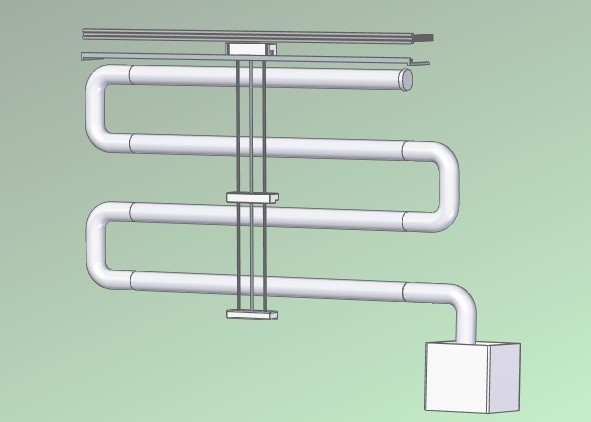
\includegraphics[width=0.55\textwidth]{img/ClaudioReal_simplificado.jpg}
        \caption{\textit{Representación de la estructura del cosechador automático y su entorno.}}
        \label{fig:ClaudioReal_simplificado}
\end{figure}

% Interaccion Niveles


% Flujo Informacion


% Maquina Estados Global



\section{Modelado y diseño mecánico}

\subsection{Especificaciones de diseño y restricciones}
\subsubsection{Dimensiones del área de trabajo}

El sistema robótico presenta una configuración cartesiana de dos ejes (XY), con dimensiones de 3~m de ancho por 2~m de alto, diseñado para operar sobre cultivos hidropónicos verticales dispuestos en tubos montados sobre una pared.

\subsubsection{Especificaciones cinemáticas}

Las especificaciones de velocidad, aceleración y resolución de los actuadores se detallan en la Tabla \ref{tab:esp_cinematicas}.

\begin{table}[htbp]
\centering
\begin{tabular}{|l|c|c|}
\hline
\textbf{Parámetro} & \textbf{Eje Horizontal} & \textbf{Eje Vertical} \\ \hline
Velocidad máxima [\(\frac{mm}{s}\)] & 250 & 75 \\ \hline
Velocidad mínima [\(\frac{mm}{s}\)] & 12.5 & 2.5 \\ \hline
Aceleración [\(\frac{mm}{s^2}\)] & 187.5 & 45 \\ \hline
Avance por revolución [\(\frac{mm}{rev}\)] & 40 & 8 \\ \hline
Resolución [\(\frac{pasos}{mm}\)] & 40 & 200 \\ \hline
Micropasos & 8 & 8 \\ \hline
\multicolumn{3}{c}{} \\
\end{tabular}
\caption{Especificaciones cinemáticas de los ejes de movimiento}
\label{tab:esp_cinematicas}
\end{table}

La diferencia en resolución entre ambos ejes responde a los requisitos operativos: el eje horizontal requiere mayor velocidad de desplazamiento con precisión moderada, mientras que el eje vertical necesita mayor precisión de posicionamiento con velocidades menores debido a las operaciones de elevación de carga.

\subsubsection{Cargas del sistema}

Las cargas consideradas en el diseño se distribuyen según su función operativa:\\

Cargas del eje horizontal.\\
\noindent
El motor del eje horizontal debe mover aproximadamente 12~kg, correspondiente a la suma del peso de las varillas verticales, la varilla roscada, los soportes estructurales y el brazo robótico. La carga es soportada principalmente por el perfil superior.

Cargas del eje vertical.\\
\noindent
El motor del eje vertical debe mover la carga correspondiente al peso del brazo robótico y la lechuga (aproximadamente 1.2kg). Además, debe vencer la fricción que se genera entre la tuerca y la varilla roscada.

\subsubsection{Componentes estructurales}

El robot cuenta con tres soportes estructurales principales fabricados mediante impresión 3D:

\begin{itemize}[label=$\bullet$]
    \item \underline{Soporte inferior:} Fijación de las varillas verticales y montaje del motor del eje Z
    \item \underline{Soporte medio:} Sostiene el brazo robótico y la cámara, desplazándose verticalmente mediante la varilla roscada
    \item \underline{Soporte superior:} Acoplamiento cinemático de los dos movimientos perpendiculares (horizontal y vertical), actuando como elemento de unión entre ambos subsistemas
\end{itemize}

El motor del movimiento horizontal estará sostenido por un soporte como el mostrado en la fig. \ref{fig:soporte_motor_pap}
\begin{table}[H]
\centering
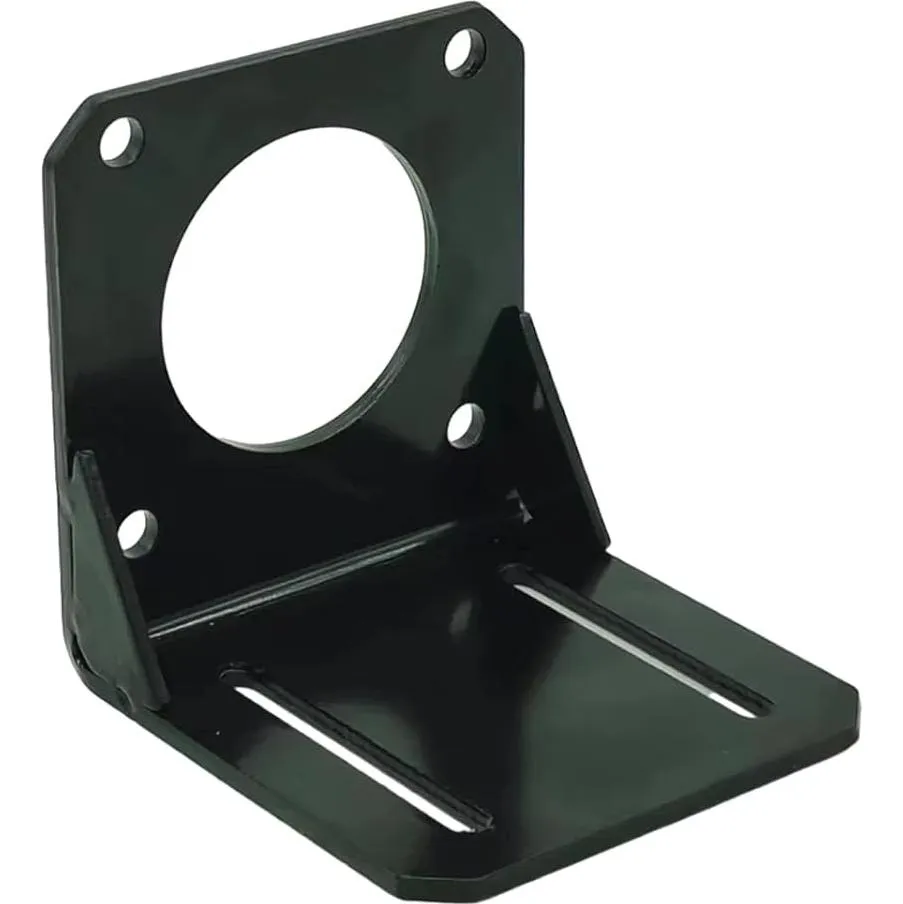
\includegraphics[width=0.25\textwidth]{img/soporte_motor_pap.png}
\caption{\textit{Referencia de oporte para motor pap.}}
\label{fig:soporte_motor_pap}
\end{table}
El perfil superior se une a un caño estructural en cada extremo utilizando soportes tipo L. Mientras que el perfil lateral que brinda rigidez, se atornilla también a un tramo de caño estructural en cada extremo. Las orientaciones de los caños estructurales de soporte se puede observar en la fig. \ref{fig:ClaudioReal_simplificado}

%\subsection{Análisis Cinemático del Sistema}
%% Grados Libertad


%% Ecuaciones Movimiento


%% Espacio Trabajo



%\subsection{Diseño Estructural}
%% Calculos Resistencia


\subsection{Sistema de movimiento horizontal}
\subsubsection{Selección del perfil de movimiento horizontal}
Se selecciona un perfil de aluminio V-Slot con ruedas de precisión, que ofrece:
\begin{itemize}[label=$\bullet$]
    \item Capacidad de carga de hasta 50\,kg
    \item Sistema de ajuste para eliminación de juego mecánico
    \item Alta precisión de movimiento
\end{itemize}

Cálculo de deflexión \\
\noindent
Para verificar la rigidez del perfil, se analiza como una viga simplemente apoyada bajo carga centrada:
\begin{equation}
\delta = \frac{F \cdot L^3}{48 \cdot E \cdot I}
\label{eq:deflexion_perfil}
\end{equation}

donde:
\begin{itemize}[label=$\bullet$]
    \item $E = 69\,000$\,N/mm$^2$ (módulo de Young del aluminio)
    \item $L = 3\,000$\,mm (longitud del perfil)
    \item $I$ = momento de inercia del perfil
    \item $F$ = carga aplicada
\end{itemize}

Para un perfil V-Slot 20$\times$80\,mm, con $I = 350\,000$\,mm$^4$, la deflexión calculada es:
\[\delta = 0.87\,\text{mm}\]

Este valor es aceptable considerando que representa menos del 0.03\% de la longitud total del perfil, cumpliendo con criterios de rigidez para aplicaciones de precisión moderada.

Como complemento, se seleccionan dos carros lineales estándar de 100\,mm de ancho, cada uno equipado con 4 ruedas tipo DELRIN que se desplazan sobre el perfil V-Slot.
\begin{figure}[H]
    \centering
    \begin{subfigure}{0.35\textwidth}
        \centering
        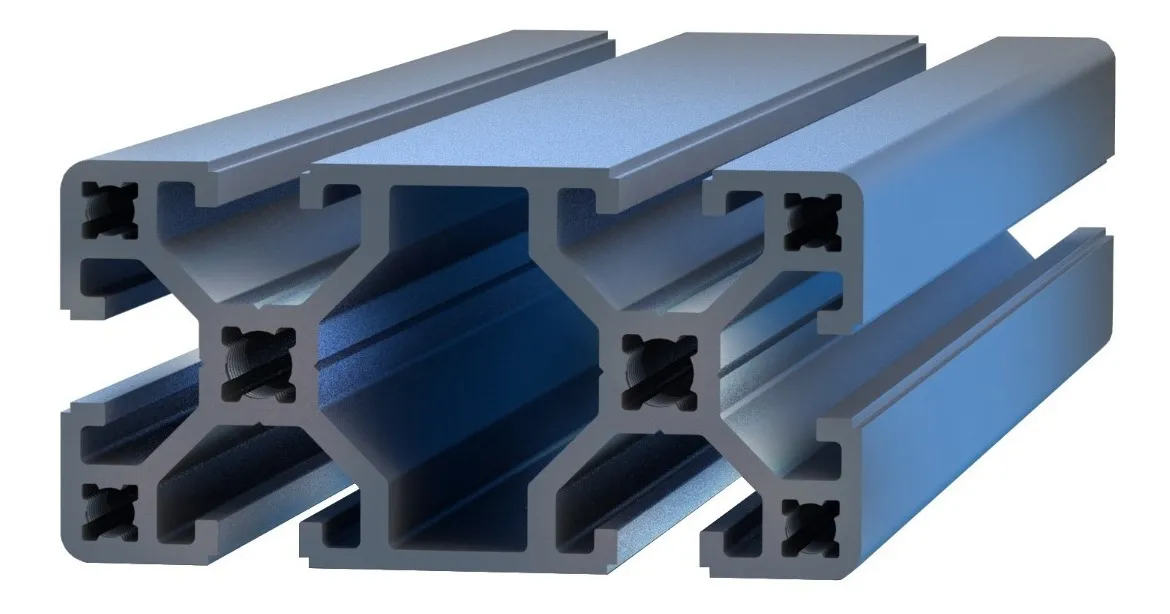
\includegraphics[width=0.7\textwidth]{img/vslot_40x80.png}
        \caption{\textit{Perfil v-slot.}}
        \label{fig:vslot_40x80}
    \end{subfigure}
    \hspace{0.5cm}
    \begin{subfigure}{0.35\textwidth}
        \centering
        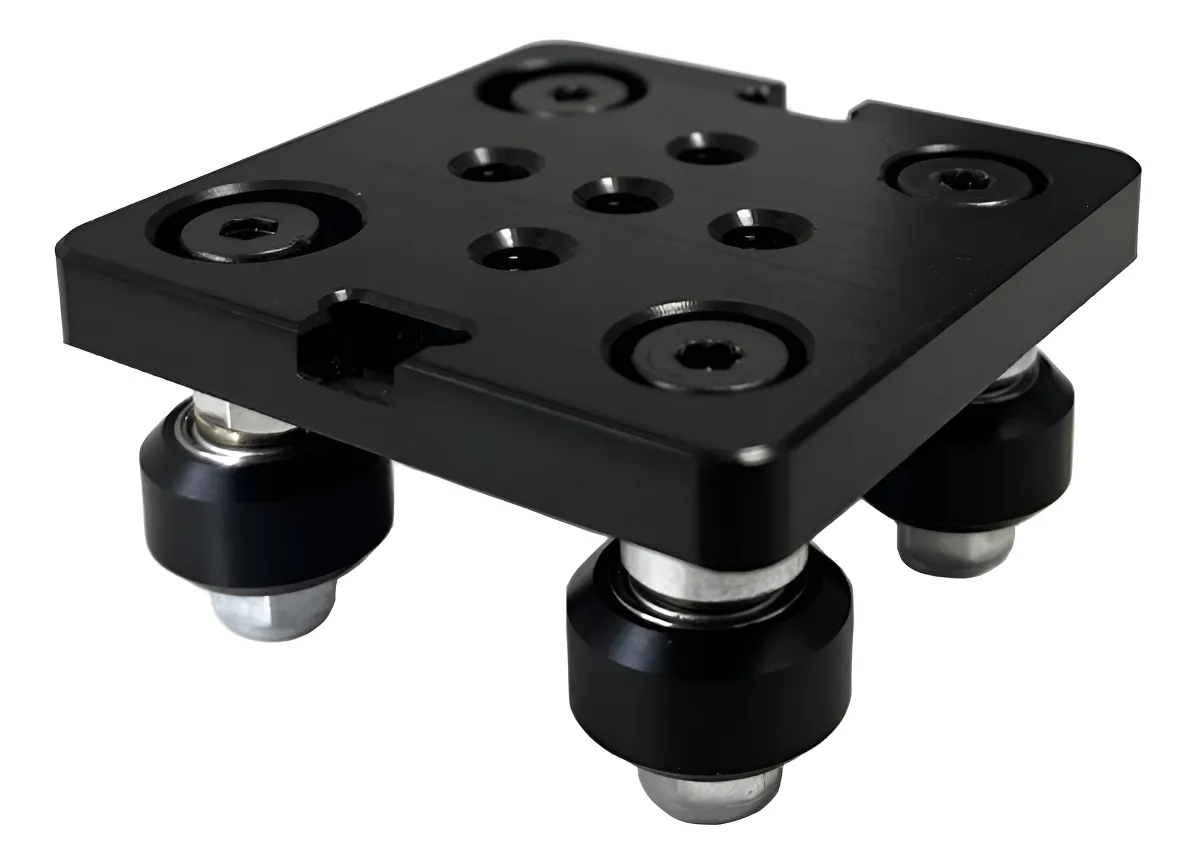
\includegraphics[width=0.4\textwidth]{img/carro_perfilvslot.png}
        \caption{\textit{Sistema de ruedas para deslizamiento sobre perfil v-slot.}}
        \label{fig:carro_perfilvslot}
    \end{subfigure}
    \caption{\textit{Sistema de deslizamiento con perfil v-slot.}}
\end{figure}
Al activarse los motores del robot serie se genera una fuerza F1 como la que se muestra en \ref{fig:esfuerzo_lateral}. Dicha fuerza genera que toda la estructura vertical se mueva hacia atras.
\begin{figure}[H]
        \centering
        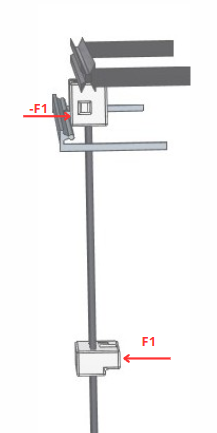
\includegraphics[width=0.3\textwidth]{img/esfuerzo_lateral.png}
        \caption{\textit{Analisis cualitativo de fuerzas.}}
        \label{fig:esfuerzo_lateral}
\end{figure}
Para eliminar ese movimiento se coloca un perfil como el de la fig \ref{fig:barra_lateral}, en conjunto con sus rodamientos (fig. \ref{fig:sbr20uu}) acoplados al soporte superior. De esta manera se genera una fuerza semejante a F1 pero en sentido contrario.
\begin{figure}[H]
    \centering
    \begin{subfigure}{0.35\textwidth}
        \centering
        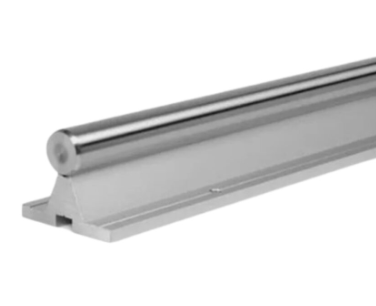
\includegraphics[width=0.7\textwidth]{img/barra_lateral.png}
        \caption{\textit{Barra lateral.}}
        \label{fig:barra_lateral}
    \end{subfigure}
    \hspace{0.5cm}
    \begin{subfigure}{0.35\textwidth}
        \centering
        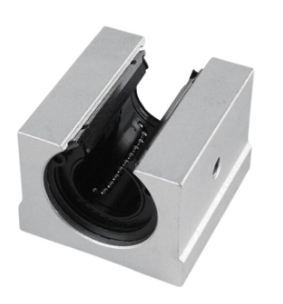
\includegraphics[width=0.65\textwidth]{img/sbr20uu.png}
        \caption{\textit{Carro para deslizamiento sobre barra lateral.}}
        \label{fig:sbr20uu}
    \end{subfigure}
    \caption{Sistema de rigidez horizontal.}
\end{figure}


\subsubsection{Sistema de transmisión por correa}
El sistema utiliza correa dentada GT2 con poleas de igual diámetro en ambos extremos. La longitud de correa necesaria se calcula como:
\begin{equation}
L = 2C + \pi D = 6.06\,\text{m}
\label{eq:longitud_correa}
\end{equation}
donde $C$ es la distancia entre centros de las poleas y $D$ el diámetro de las mismas. \\

Distribución de cargas en el sistema\\
\noindent
La carga total de 12.72\,kg se distribuye entre dos subsistemas mecánicos:

\begin{itemize}[label=$\bullet$]
    \item \underline{Carga soportada por el perfil V-Slot:} El perfil y los carros lineales soportan directamente el peso vertical de la carga (8.96\,kg) a través de las ruedas DELRIN. Esta carga genera únicamente esfuerzos de compresión y flexión en el perfil, sin afectar directamente al sistema de transmisión.
    
    \item \underline{Carga dinámica del motor:} El motor debe vencer las fuerzas necesarias para acelerar y mover horizontalmente la masa efectiva del sistema (12.72\,kg). Esta masa efectiva es menor que la carga total debido a que:
    \begin{enumerate}
        \item Las ruedas del carro transforman el rozamiento estático en rodadura, reduciendo significativamente la resistencia al movimiento
        \item El perfil V-Slot absorbe las cargas verticales, dejando al motor únicamente las fuerzas inerciales horizontales y las fricciones residuales del sistema
    \end{enumerate}
\end{itemize}

Esta distribución asume un coeficiente de fricción por rodadura de $\mu_{\text{rod}} \approx 0.001$ para ruedas DELRIN sobre aluminio.\\ \\
Selección polea y correa\\
\noindent
Se selecciona una polea GT2 de 40 dientes y diametro de 25.5mm que tiene 80mm/rev

\begin{enumerate}
    \item \underline{Precisión de posicionamiento}: El desplazamiento lineal por revolución determina la resolución del sistema:
    \begin{equation}
    \text{Resolución} = \frac{P}{n_{\text{pasos/rev}}} = 0.05mm/paso
    \end{equation}
    donde P=80mm/rev, $n_{\text{pasos/rev}} = 200 \times 8 = 1600$ pasos (con 8 micropasos). Esto implica 20 pasos/mm.
    \item \underline{Velocidad de operación}: Para una velocidad lineal objetivo de $v_{\text{max}} = 250$\,mm/s, la velocidad angular requerida es:
    \begin{equation}
    n = \frac{v_{\text{max}}}{P} \times 60 = 187.5 [\text{RPM}] 
    \end{equation}
    Velocidad que se encuentra en la zona de torque máximo.
\end{enumerate}
Para esta polea, se selecciona una correa dentada de 10mm de ancho.\\

Análisis de fuerzas\\
Para determinar el torque motor requerido, se consideran las siguientes fuerzas resistivas:

\begin{enumerate}
    \item \underline{Fricción por rodadura:}
    \begin{equation}
    F_{\text{rod}} = \mu_{\text{rodadura}} \cdot m \cdot g \cdot \frac{1}{r_{\text{rueda}}}= 0.021N
    \end{equation}
    donde $\mu_{\text{rodadura}}$ depende del material de las ruedas DELRIN sobre aluminio.
    
    \item \underline{Fuerza de aceleración:}
    \begin{equation}
    F_{\text{acel}} = (m_{\text{carga}} + m_{\text{correa}}) \cdot a_{\text{max}} = 2.43 N
    \end{equation}
    Incluye la masa de la carga útil y la masa lineal de la correa GT2.
    
    \item \underline{Fricción en rodamientos de poleas:}
    \begin{equation}
    F_{\text{friccion\_rod}} = T_{\text{correa}} \cdot \mu_{\text{rodamientos}} \cdot n = 0.12N
    \end{equation}
    con $n = 2$ (polea conducida y tensor).
    
    \item \underline{Fuerza interna de la correa:}
    \begin{equation}
    F_{\text{correa}} = 0.5\,\text{N}
    \end{equation}
    Valor empírico para correas GT2 según especificaciones del fabricante.
    
    \item \underline{Otras pérdidas:}
    \begin{equation}
    F_{\text{otras}} = 0.1 \cdot (F_{\text{acel}} + F_{\text{rod}})=0.26N
    \end{equation}
    Se estima un 10\% adicional para pérdidas no modeladas.
\end{enumerate}

Cálculo del torque motor\\
Considerando la distribución de cargas analizada anteriormente, donde el motor debe mover la masa total (12.72\,kg), la fuerza total requerida en la base del sistema es:
\begin{equation}
F_{\text{tbase}} = 3.33\,\text{N}
\end{equation}


Aplicando un factor de seguridad de 2.5 para contemplar condiciones adversas de operación y degradación del sistema con el uso, el torque motor necesario resulta:
\begin{equation}
T_{\text{motor}} = F_{\text{tbase}} \cdot 2.5 \cdot r_{\text{polea}} \approx 0.1\,\text{Nm}
\label{eq:torque_motor}
\end{equation}

Selección del motor\\
Se selecciona un motor paso a paso NEMA 17. Analizando la curva dinámica torque-velocidad (Figura~\ref{fig:Curva_din_nema34}), se verifica que para la velocidad máxima de operación de 250\,mm/s (187.5\,rpm), el torque disponible supera ampliamente el requerimiento calculado de 0.1\,Nm, garantizando un margen de seguridad adecuado para la operación continua del sistema. 
\begin{figure}[H]
    \centering
    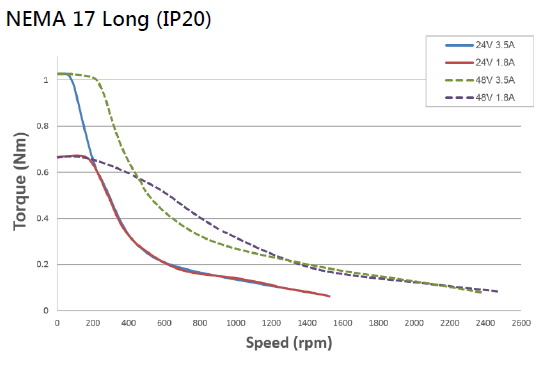
\includegraphics[width=0.65\textwidth]{img/Nema17.png}
    \caption{\textit{Curva dinámica torque-velocidad del motor paso a paso NEMA 17.}}
    \label{fig:Curva_din_nema17}
\end{figure}

%% Calculo Cargas Horizontal



\subsection{Sistema de movimiento vertical}
\subsubsection{Selección de varilla trapezoidal} 
\label{sec:mov_vertical}
El sistema de elevación vertical debe soportar una carga total de 1.2\,kg (lechuga y accesorios) a lo largo de una varilla de 2\,m de longitud. La varilla está fijada por su extremo superior y la carga se desplaza a lo largo de ella mediante una tuerca, trabajando por lo tanto a tracción. Se adopta un factor de seguridad de 4 para contemplar cargas dinámicas, desalineaciones y degradación del sistema con el uso.

Aunque la varilla trabaja principalmente a tracción, es necesario verificar la estabilidad estructural frente a posibles cargas de compresión durante maniobras o situaciones no previstas. Considerando que la varilla tiene ambos extremos empotrados, la carga crítica de Euler se calcula como:

\begin{equation}
P_{\text{cr}} = \frac{\pi^2 \cdot E \cdot I}{(K \cdot L)^2}
\label{eq:euler_pandeo}
\end{equation}

donde:
\begin{itemize}[label=$\bullet$]
    \item $E = 200$\,GPa = 200\,000\,N/mm$^2$ (módulo de Young del acero)
    \item $I$ = momento de inercia de la sección transversal de la varilla
    \item $L = 2\,000$\,mm (longitud de la varilla)
    \item $K = 0.5$ (factor de longitud efectiva para ambos extremos empotrados)
\end{itemize}

La carga admisible debe satisfacer:
\begin{equation}
P_{\text{adm}} = \frac{P_{\text{cr}}}{FS} > W
\end{equation}

donde $W = m \cdot g = 1.2\,\text{kg} \cdot 9.81\,\text{m/s}^2 = 11.77$\,N es el peso a soportar, y $FS = 4$ es el factor de seguridad adoptado.

Por lo tanto:
\[P_{\text{adm}} > 11.77\,\text{N} \cdot 4 = 47.08\,\text{N}\]

Selección del diámetro.\\
\noindent
Tras evaluar diferentes diámetros comerciales de varillas trapezoidales de acero, se selecciona una varilla TR16$\times$8 (diámetro nominal 16\,mm, paso 8\,mm).

Para una varilla de diámetro exterior $d_e = 16$\,mm, el momento de inercia de la sección circular es:
\[I = \frac{\pi \cdot d_e^4}{64} = \frac{\pi \cdot 16^4}{64} = 3\,217\,\text{mm}^4\]

Sustituyendo en la ecuación~(\ref{eq:euler_pandeo}) con $K = 0.5$ para extremos empotrados:
\[P_{\text{cr}} = \frac{\pi^2 \cdot 200\,000\,\text{N/mm}^2 \cdot 3\,217\,\text{mm}^4}{(0.5 \cdot 2\,000\,\text{mm})^2} = \frac{6\,341\,481\,520}{1\,000\,000} = 6\,341\,\text{N}\]

La carga admisible resulta:
\[P_{\text{adm}} = \frac{6\,341\,\text{N}}{4} = 1\,585\,\text{N} > 47.08\,\text{N}\]

Se verifica que la varilla seleccionada cumple ampliamente con los requerimientos de resistencia, proporcionando un margen de seguridad de aproximadamente 33.7 veces la carga mínima requerida, garantizando la integridad estructural del sistema incluso ante condiciones adversas.

\begin{figure}[H]
    \centering
    \begin{subfigure}{0.35\textwidth}
        \centering
        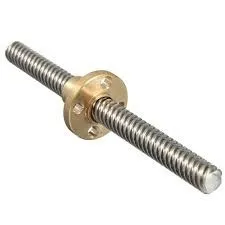
\includegraphics[width=0.7\textwidth]{img/v_roscada.png}
        \caption{\textit{Varilla trapezoidal 16x8.}}
        \label{fig:v_roscada}
    \end{subfigure}
    \hspace{0.5cm}
    \begin{subfigure}{0.35\textwidth}
        \centering
        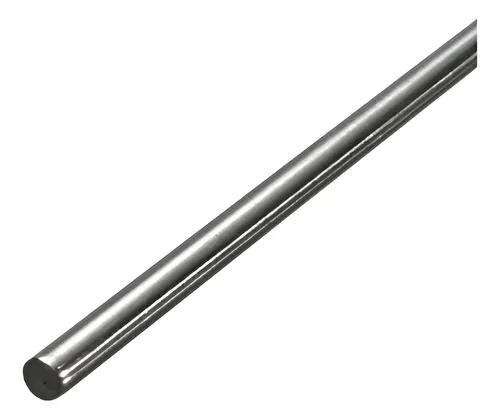
\includegraphics[width=0.7\textwidth]{img/varilla lisa.png}
        \caption{\textit{Varilla de acero maciza de 16mm de diametro.}}
        \label{fig:varilla lisa}
    \end{subfigure}
    \caption{\textit{Sistema de transmisión vertical.}}
\end{figure}

El sistema debe operar con los siguientes parámetros:
\begin{itemize}[label=$\bullet$]
    \item Velocidad lineal máxima: 75\,mm/s
    \item Paso de varilla: 8\,mm
    \item Velocidad angular (pasos completos): $\omega = \frac{v_{\text{lineal}}}{\text{paso}} \cdot 60 = \frac{75\,\text{mm/s}}{8\,\text{mm}} \cdot 60 \approx 562.5$\,rpm
    \item Microstepping: 1/8 paso (1\,600 pasos/revolución)
    \item Resolución: $\frac{1\,600\,\text{pasos/rev}}{8\,\text{mm/rev}} = 200$\,pasos/mm
\end{itemize}

El uso de microstepping 1/8 permite mantener una alta resolución de 200\,pasos/mm (equivalente a 0.005\,mm o 5\,micrones por paso) mientras se opera a baja velocidad, maximizando el torque disponible del motor y proporcionando un movimiento suave y preciso.\\
%\subsubsection{Cálculo de torque y selección del motor}
\subsubsection{Cálculo de torque motor para accionamiento vertical}

El torque requerido para mover una carga mediante una varilla trapezoidal se compone de dos componentes: el torque necesario para vencer la fricción en la rosca y el torque para vencer la fricción en el collarín del soporte. Dicho torque se calcula a partir de la ecuación \ref{eq:torque_total_varilla}

donde:
\begin{itemize}[label=$\bullet$]
    \item $F = 1.2\,\text{kg} \cdot 9.81\,\text{m/s}^2 = 11.77$\,N
    \item $d_m = 14$\,mm
    \item $d_c \approx 26$\,mm
    \item $\mu_c = 0.2$
    \item $k_R = 1.5$ (para paso de 8\,mm, ángulo de hélice $\approx 10.3^\circ$)
    \item $k_L = 0.5$ (para paso de 8\,mm)
\end{itemize}

Sustituyendo valores en las ecuaciones~(\ref{eq:torque_subida}) y~(\ref{eq:torque_bajada}):

\[T_{\text{subida}} = \frac{11.77 \cdot 14}{2} \cdot 1.5 + \frac{11.77 \cdot 0.2 \cdot 26}{2} = 123.6 + 30.6 = 154.2\,\text{Nmm}\]

\[T_{\text{bajada}} = \frac{11.77 \cdot 14}{2} \cdot 0.5 + \frac{11.77 \cdot 0.2 \cdot 26}{2} = 41.2 + 30.6 = 71.8\,\text{Nmm}\]

El torque de diseño se toma como el mayor de ambos:
\[T_{\text{base}} = \max(T_{\text{subida}}, T_{\text{bajada}}) = 154.2\,\text{Nmm} = 0.154\,\text{Nm}\]

Se aplican los siguientes factores correctivos:

\begin{enumerate}
    \item \underline{Factor por fricción adicional en roscas trapezoidales ($f_1 = 2.0$)}: Las roscas trapezoidales presentan pérdidas significativas por fricción que no están completamente capturadas en las ecuaciones simplificadas. Estas pérdidas se deben a:
    \begin{itemize}[label=$\bullet$]
        \item La geometría de los canales trapezoidales, que generan mayor área de contacto y fricción entre los flancos de la rosca y la tuerca
        \item El efecto de acuñamiento de la rosca durante el movimiento, especialmente pronunciado en roscas trapezoidales comparado con roscas de bolas
        \item El roce continuo metal-metal entre la tuerca y toda la longitud de la rosca, que genera calentamiento y puede aumentar la fricción
        \item Pérdidas adicionales por desalineación a lo largo de los 2\,m de varilla
        \item Variaciones en la calidad de la lubricación durante la vida útil del sistema
    \end{itemize}
    El paso de 8\,mm reduce este factor respecto a pasos menores debido a la menor cantidad de vueltas necesarias para el mismo desplazamiento lineal, disminuyendo las pérdidas acumulativas por fricción.

    \item \underline{Factor de seguridad por caída de torque con velocidad ($f_2 = 1.2$):} Los motores paso a paso experimentan una reducción significativa del torque disponible al aumentar la velocidad de rotación, como se observa en las curvas dinámicas. Dado que el sistema opera a baja velocidad (70.3\,rpm), el motor mantiene la mayor parte de su torque nominal, requiriendo un factor de seguridad menor.
\end{enumerate}

El torque motor requerido resulta:
\begin{equation}
T_{\text{motor}} = T_{\text{base}} \cdot f_1 \cdot f_2 = 0.154 \cdot 2.0 \cdot 1.2 = 0.37\,\text{Nm}
\label{eq:torque_motor_vertical}
\end{equation}

\subsubsection{Selección del motor paso a paso}
Considerando la velocidad de operación de 70.3\,rpm (con microstepping 1/8), se verifica en la curva dinámica torque-velocidad (Figura~\ref{fig:Curva_din_nema34}) que se requiere un torque disponible de al menos 0.37\,Nm.

Se selecciona un motor \textbf{NEMA 34 Medium} con las siguientes especificaciones:
\begin{itemize}[label=$\bullet$]
    \item Alimentación: 24\,V / 4.5\,A
    \item Torque de retención (holding torque): $>$ 3\,Nm
    \item Torque a 70.3\,rpm: $\approx$ 2.5\,Nm (según curva dinámica)
\end{itemize}

El motor seleccionado proporciona un margen de seguridad de aproximadamente 6.76 veces el torque requerido a la velocidad de operación, garantizando movimientos suaves y seguros durante toda la operación del sistema, incluyendo situaciones de carga máxima y fricción elevada. La baja velocidad de operación permite aprovechar el torque máximo disponible del motor, resultando en un diseño robusto y confiable.

\begin{figure}[H]
    \centering
    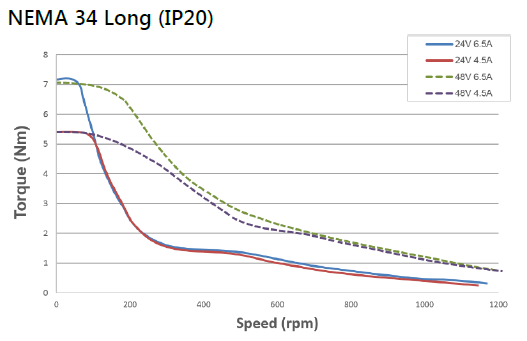
\includegraphics[width=0.65\textwidth]{img/Nema34.png}
    \caption{\textit{Curva dinámica torque-velocidad del motor paso a paso NEMA 34 Medium.}}
    \label{fig:Curva_din_nema34}
\end{figure}

%% Seleccion Guias



\subsection{Robot serie}
Se cuenta con un brazo de dos grados de libertad controlables para el posicionamiento del efector final que es de tipo pinza.

\subsubsection{Descripción del Sistema}

El brazo robótico consiste en una configuración planar de dos eslabones articulados mediante juntas rotacionales, con un efector final tipo gripper de pinza. Este sistema posee dos grados de libertad en el plano, definidos por los ángulos de rotación $\theta_1$ y $\theta_2$ de cada articulación.

\subsubsection{Parámetros Geométricos}

\begin{itemize}
    \item $L_1$: Longitud del primer eslabón (eslabón proximal)
    \item $L_2$: Longitud del segundo eslabón (eslabón distal)
    \item $\theta_1$: Ángulo de la primera articulación (base)
    \item $\theta_2$: Ángulo de la segunda articulación (codo)
\end{itemize}

\subsubsection{Cinemática Directa}

La cinemática directa establece la relación entre las coordenadas articulares $(\theta_1, \theta_2)$ y la posición del efector final $(x, y)$ en el plano.

La posición del efector final se calcula mediante:

\begin{align}
    x &= L_1 \cdot \cos(\theta_1) + L_2 \cdot \cos(\theta_1 + \theta_2) \\
    y &= L_1 \cdot \sin(\theta_1) + L_2 \cdot \sin(\theta_1 + \theta_2)
\end{align}

La orientación del efector final está dada por:

\begin{equation}
    \phi = \theta_1 + \theta_2
\end{equation}

\subsubsection{Cinemática Inversa}

La cinemática inversa determina los ángulos articulares necesarios para alcanzar una posición deseada $(x_d, y_d)$. Este problema presenta dos soluciones posibles (configuración de codo arriba y codo abajo).

Primero se calcula el ángulo $\theta_2$:

\begin{equation}
    \cos(\theta_2) = \frac{x_d^2 + y_d^2 - L_1^2 - L_2^2}{2 \cdot L_1 \cdot L_2}
\end{equation}

\begin{equation}
    \theta_2 = \pm \arccos\left(\frac{x_d^2 + y_d^2 - L_1^2 - L_2^2}{2 \cdot L_1 \cdot L_2}\right)
\end{equation}

Luego se determina $\theta_1$:

\begin{equation}
    \theta_1 = \arctan2(y_d, x_d) - \arctan2(L_2 \cdot \sin(\theta_2), L_1 + L_2 \cdot \cos(\theta_2))
\end{equation}

\subsubsection{Espacio de Trabajo}

El espacio de trabajo accesible para el efector final es un anillo circular con:

\begin{itemize}
    \item Radio máximo: $R_{max} = L_1 + L_2$ (brazo completamente extendido)
    \item Radio mínimo: $R_{min} = |L_1 - L_2|$ (brazo completamente plegado)
\end{itemize}

\subsubsection{Jacobiano}

El Jacobiano relaciona las velocidades articulares con las velocidades del efector final:

\begin{equation}
    \begin{bmatrix}
        \dot{x} \\
        \dot{y}
    \end{bmatrix}
    =
    \begin{bmatrix}
        J_{11} & J_{12} \\
        J_{21} & J_{22}
    \end{bmatrix}
    \begin{bmatrix}
        \dot{\theta}_1 \\
        \dot{\theta}_2
    \end{bmatrix}
\end{equation}

Donde:

\begin{align}
    J_{11} &= -L_1 \cdot \sin(\theta_1) - L_2 \cdot \sin(\theta_1 + \theta_2) \\
    J_{12} &= -L_2 \cdot \sin(\theta_1 + \theta_2) \\
    J_{21} &= L_1 \cdot \cos(\theta_1) + L_2 \cdot \cos(\theta_1 + \theta_2) \\
    J_{22} &= L_2 \cdot \cos(\theta_1 + \theta_2)
\end{align}

\subsubsection{Gripper Tipo Pinza}

El gripper se ubica en el extremo del segundo eslabón y posee un grado de libertad adicional (no considerado en los 2 GDL principales) para la apertura/cierre de las mandíbulas, controlado por el parámetro $d$ (distancia entre mandíbulas).

\subsubsection{Singularidades}

El sistema presenta singularidades cuando el determinante del Jacobiano es cero:

\begin{equation}
    \det(J) = L_1 \cdot L_2 \cdot \sin(\theta_2) = 0
\end{equation}

Esto ocurre cuando \(\theta_2 = 0^\circ \) o \(\theta_2 = 180^\circ\), es decir, cuando el brazo está completamente extendido o plegado.


%\subsection{Cinemática en el espacio articular}

En esta sección se aborda el análisis cinemático de un manipulador robótico serie de dos grados de libertad operando exclusivamente en el espacio articular. Este enfoque permite un control directo sobre las variables articulares del sistema, evitando la necesidad de resolver transformaciones al espacio cartesiano.

\subsubsection{Definición del espacio de configuraciones}

El estado del manipulador queda completamente determinado por el vector de coordenadas articulares:

\begin{equation}
\mathbf{q} = \begin{bmatrix} \theta_1 \\ \theta_2 \end{bmatrix}
\end{equation}

donde $\theta_1$ y $\theta_2$ representan los ángulos de las articulaciones 1 y 2 respectivamente, medidos en sus sistemas de referencia locales.

El procedimiento implementado para el control cinemático en espacio articular se desarrolla según los siguientes pasos:

\begin{enumerate}
    \item \textbf{Definición de consigna}: Se especifica el vector de configuración deseado $\mathbf{q}_d = [\theta_{1d}, \theta_{2d}]^T$, estableciendo directamente los valores angulares objetivo para cada articulación.
    
    \item \textbf{Envío de comandos}: Los valores angulares se transmiten como señales de control a los actuadores correspondientes de cada eslabón.
    
    \item \textbf{Verificación de posición}: Se evalúa si la configuración alcanzada corresponde a la pose deseada del efector final, mediante observación directa o retroalimentación sensorial.
\end{enumerate}

La implementación del control cinemático en el espacio articular presenta las siguientes ventajas operativas:

\begin{itemize}
    \item \textbf{Simplicidad computacional}: Se elimina la necesidad de resolver el problema de cinemática inversa, el cual puede presentar múltiples soluciones o complejidad analítica considerable.
    
    \item \textbf{Control directo}: Los comandos se envían directamente a los actuadores sin transformaciones intermedias, reduciendo la latencia del sistema.
    
    \item \textbf{Evitación de singularidades}: Al operar en el espacio de configuraciones, se evitan las singularidades cinemáticas inherentes al espacio cartesiano.
    
    \item \textbf{Predictibilidad}: El comportamiento del sistema es determinista y predecible para cualquier configuración dentro del espacio de trabajo articular.
\end{itemize}

\subsection{Limitaciones}

Si bien el enfoque presenta ventajas significativas, es importante señalar que la planificación de trayectorias en el espacio cartesiano requiere de la transformación mediante la cinemática directa para verificar que las configuraciones articulares seleccionadas efectivamente posicionan el efector final en las coordenadas espaciales deseadas.
\subsubsection{Dinámica de robot serie de 2 GDL}
Para el análisis dinámico de la estructura multiarticular de 2 grados de libertad (2-GDL), se emplea la formulación de Euler-Lagrange. Este método energético resulta particularmente eficiente para sistemas de cuerpos rígidos articulados, ya que evita el cálculo explícito de fuerzas de reacción internas y permite obtener directamente las ecuaciones de movimiento en términos de las coordenadas generalizadas.

El lagrangiano del sistema se define como:
\begin{equation}
\mathcal{L} = K - U
\end{equation}
donde $K$ es la energía cinética total y $U$ es la energía potencial total del sistema.

Las ecuaciones de movimiento se obtienen mediante las ecuaciones de Euler-Lagrange:
\begin{equation}
\tau_i = \frac{d}{dt}\left(\frac{\partial \mathcal{L}}{\partial \dot{\theta}_i}\right) - \frac{\partial \mathcal{L}}{\partial \theta_i}
\end{equation}
donde $\tau_i$ representa el torque aplicado en la articulación $i$ y $\theta_i$ son las coordenadas generalizadas (ángulos de rotación).


El sistema consiste en dos eslabones rígidos conectados en serie mediante articulaciones rotacionales. La configuración y parámetros se describen a continuación:
\begin{itemize}[label=$\bullet$]
    \item $L_1$: Longitud total del eslabón 1
    \item $L_2$: Longitud total del eslabón 2
    \item $l_1$: Distancia desde la articulación 1 al centro de masa del eslabón 1
    \item $l_2$: Distancia desde la articulación 2 al centro de masa del eslabón 2
    \item $m_1$, $m_2$: Masas de los eslabones 1 y 2
    \item $I_1$, $I_2$: Momentos de inercia de los eslabones respecto a sus centros de masa
\end{itemize}

\textbf{Coordenadas generalizadas:}
\begin{itemize}[label=$\bullet$]
    \item $\theta_1$: Ángulo de rotación de la articulación 1 (respecto al eje horizontal)
    \item $\theta_2$: Ángulo de rotación de la articulación 2 (respecto al eje horizontal)
\end{itemize}
\begin{figure}[H]
    \centering
    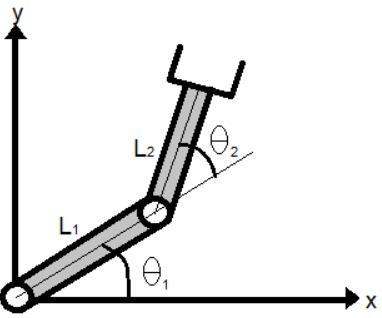
\includegraphics[width=0.4\textwidth]{img/DCL_brazo.png}
    \caption{\textit{Diagrama cinemático y de eslabones del manipulador robótico planar}}
    \label{fig:DCL_brazo}
\end{figure}

Energía potencial eslabón 1:\\
\noindent
La energía potencial gravitacional del eslabón 1 está dada por:
\begin{equation}
U_1 = m_1 \cdot g \cdot l_1 \cdot \sin(\theta_1)
\end{equation}

donde $g$ es la aceleración de la gravedad y la altura del centro de masa se mide desde un nivel de referencia horizontal.\\

Energía cinética eslabón 1:\\
\noindent
La energía cinética del eslabón 1 tiene dos componentes: rotacional y traslacional.
\begin{equation}
K_1 = \frac{1}{2} I_1 \dot{\theta}_1^2 + \frac{1}{2} m_1 v_1^2
\end{equation}

Para calcular $v_1^2$, determinamos primero la posición del centro de masa del eslabón 1 y derivando respecto al tiempo:

\noindent
\begin{minipage}{0.48\textwidth}
\begin{align}
x_1 &= l_1 \cos(\theta_1) \\
y_1 &= l_1 \sin(\theta_1)
\end{align}
\end{minipage}
\hfill
\begin{minipage}{0.48\textwidth}
\begin{align}
\dot{x}_1 &= -l_1 \sin(\theta_1) \dot{\theta}_1 \\
\dot{y}_1 &= l_1 \cos(\theta_1) \dot{\theta}_1
\end{align}
\end{minipage}

La velocidad al cuadrado del centro de masa es:
\begin{equation}
v_1^2 = \dot{x}_1^2 + \dot{y}_1^2 = l_1^2\sin^2(\theta_1)\dot{\theta}_1^2 + l_1^2\cos^2(\theta_1)\dot{\theta}_1^2 = l_1^2\dot{\theta}_1^2
\end{equation}

Por lo tanto, la energía cinética del eslabón 1 queda:
\begin{equation}
K_1 = \frac{1}{2}(m_1l_1^2 + I_1)\dot{\theta}_1^2
\end{equation}

Energía potencial eslabón 2:\\
\noindent
La energía potencial del eslabón 2 considera la altura de su centro de masa, que depende de ambos ángulos:
\begin{equation}
U_2 = m_2 \cdot g \cdot (L_1 \sin(\theta_1) + l_2 \sin(\theta_2))
\end{equation}

El primer término representa la contribución de la articulación 1, mientras que el segundo término corresponde a la posición del centro de masa del eslabón 2 respecto a la articulación 2.\\

Energía cinética eslabón 2:\\
\noindent
La energía cinética del eslabón 2 es:
\begin{equation}
K_2 = \frac{1}{2} I_2 \dot{\theta}_2^2 + \frac{1}{2} m_2 v_2^2
\end{equation}

La posición del centro de masa del eslabón 2 es: \\
\noindent
\begin{minipage}{0.48\textwidth}
\begin{align}
x_2 &= L_1\cos(\theta_1) + l_2\cos(\theta_2) \\
y_2 &= L_1\sin(\theta_1) + l_2\sin(\theta_2)
\end{align}
\end{minipage}
\hfill
\begin{minipage}{0.48\textwidth}
\begin{align}
\dot{x}_1 &= -l_1 \sin(\theta_1) \dot{\theta}_1 \\
\dot{y}_1 &= l_1 \cos(\theta_1) \dot{\theta}_1
\end{align}
\end{minipage} 

Reemplazando x e y y sus derivadas se puede obtener $v_2^2$:
%\begin{multline}
%v_2^2 = \dot{x}_2^2 + \dot{y}_2^2 = (L_1\sin(\theta_1)\dot{\theta}_1 + l_2\sin(\theta_2)\dot{\theta}_2)^2 + (L_1\cos(\theta_1)\dot{\theta}_1 + l_2\cos(\theta_2)\dot{\theta}_2)^2
%\end{multline}

%Expandiendo:
%\begin{multline}
%v_2^2 = L_1^2\sin^2(\theta_1)\dot{\theta}_1^2 + l_2^2\sin^2(\theta_2)\dot{\theta}_2^2 + 2L_1l_2\sin(\theta_1)\sin(\theta_2)\dot{\theta}_1\dot{\theta}_2 \\
%+ L_1^2\cos^2(\theta_1)\dot{\theta}_1^2 + l_2^2\cos^2(\theta_2)\dot{\theta}_2^2 + 2L_1l_2\cos(\theta_1)\cos(\theta_2)\dot{\theta}_1\dot{\theta}_2
%\end{multline}

%Agrupando términos y aplicando la identidad trigonométrica $\sin^2(\alpha) + \cos^2(\alpha) = 1$:
%\begin{equation}
%v_2^2 = L_1^2\dot{\theta}_1^2 + l_2^2\dot{\theta}_2^2 + 2L_1l_2\dot{\theta}_1\dot{\theta}_2[\sin(\theta_1)\sin(\theta_2) + \cos(\theta_1)\cos(\theta_2)]
%\end{equation}

%Utilizando la identidad del coseno de la diferencia:
%\begin{equation}
%\cos(\theta_1 - \theta_2) = \cos(\theta_1)\cos(\theta_2) + \sin(\theta_1)\sin(\theta_2)
%\end{equation}
\begin{equation}
v_2^2 = L_1^2\dot{\theta}_1^2 + l_2^2\dot{\theta}_2^2 + 2L_1l_2\dot{\theta}_1\dot{\theta}_2\cos(\theta_1 - \theta_2)
\end{equation}

Por lo tanto, la energía cinética del eslabón 2 es:
\begin{equation}
K_2 = \frac{1}{2}I_2\dot{\theta}_2^2 + \frac{1}{2}m_2\left[L_1^2\dot{\theta}_1^2 + l_2^2\dot{\theta}_2^2 + 2L_1l_2\dot{\theta}_1\dot{\theta}_2\cos(\theta_1 - \theta_2)\right]
\end{equation}

El lagrangiano total del sistema es:
\begin{equation}
\mathcal{L} = K_1 + K_2 - U_1 - U_2
\end{equation}

Sustituyendo las expresiones obtenidas y simplificando se tiene:
%\begin{multline}
%\mathcal{L} = \frac{1}{2}(m_1l_1^2 + I_1)\dot{\theta}_1^2 + \frac{1}{2}(m_2l_2^2 + I_2)\dot{\theta}_2^2 + \frac{1}{2}m_2L_1^2\dot{\theta}_1^2 \\
%+ m_2L_1l_2\dot{\theta}_1\dot{\theta}_2\cos(\theta_1 - \theta_2) \\
%- m_1gl_1\sin(\theta_1) - m_2g[L_1\sin(\theta_1) + l_2\sin(\theta_2)]
%\end{multline}

%Simplificando:
\begin{multline}
\mathcal{L} = \frac{1}{2}(m_1l_1^2 + m_2L_1^2 + I_1)\dot{\theta}_1^2 + \frac{1}{2}(m_2l_2^2 + I_2)\dot{\theta}_2^2 + m_2L_1l_2\dot{\theta}_1\dot{\theta}_2\cos(\theta_1 - \theta_2) \\
- g[(m_1l_1 + m_2L_1)\sin(\theta_1) + m_2l_2\sin(\theta_2)]
\end{multline}

Para la coordenada $\theta_1$:

%Se calculan las derivadas parciales necesarias para la ecuación de Euler-Lagrange:

%\begin{equation}
%\frac{\partial \mathcal{L}}{\partial \dot{\theta}_1} = (m_1l_1^2 + m_2L_1^2 + I_1)\dot{\theta}_1 + m_2L_1l_2\dot{\theta}_2\cos(\theta_1 - \theta_2)
%\end{equation}

%Derivando respecto al tiempo:
\begin{equation}
\frac{d}{dt}\left(\frac{\partial \mathcal{L}}{\partial \dot{\theta}_1}\right) = (m_1l_1^2 + m_2L_1^2 + I_1)\ddot{\theta}_1 + m_2L_1l_2\ddot{\theta}_2\cos(\theta_1 - \theta_2) - m_2L_1l_2\dot{\theta}_2\sin(\theta_1 - \theta_2)(\dot{\theta}_1 - \dot{\theta}_2)
\end{equation}

%Derivada parcial respecto a $\theta_1$:
\begin{equation}
\frac{\partial \mathcal{L}}{\partial \theta_1} = -m_2L_1l_2\dot{\theta}_1\dot{\theta}_2\sin(\theta_1 - \theta_2) - g(m_1l_1 + m_2L_1)\cos(\theta_1)
\end{equation}

Para la coordenada $\theta_2$:

%\begin{equation}
%\frac{\partial \mathcal{L}}{\partial \dot{\theta}_2} = (m_2l_2^2 + I_2)\dot{\theta}_2 + m_2L_1l_2\dot{\theta}_1\cos(\theta_1 - \theta_2)
%\end{equation}

%Derivando respecto al tiempo:
\begin{equation}
\frac{d}{dt}\left(\frac{\partial \mathcal{L}}{\partial \dot{\theta}_2}\right) = (m_2l_2^2 + I_2)\ddot{\theta}_2 + m_2L_1l_2\ddot{\theta}_1\cos(\theta_1 - \theta_2) - m_2L_1l_2\dot{\theta}_1\sin(\theta_1 - \theta_2)(\dot{\theta}_1 - \dot{\theta}_2)
\end{equation}

%Derivada parcial respecto a $\theta_2$:
\begin{equation}
\frac{\partial \mathcal{L}}{\partial \theta_2} = m_2L_1l_2\dot{\theta}_1\dot{\theta}_2\sin(\theta_1 - \theta_2) - gm_2l_2\cos(\theta_2)
\end{equation}

Aplicando las ecuaciones de Euler-Lagrange $\tau_i = \frac{d}{dt}\left(\frac{\partial \mathcal{L}}{\partial \dot{\theta}_i}\right) - \frac{\partial \mathcal{L}}{\partial \theta_i}$, se obtienen los torques requeridos en cada articulación:\\
\begin{itemize}[label=$\bullet$]
    \item \underline{Torque en la articulación 1}:
    \begin{equation}
    \tau_1 = (m_1l_1^2 + m_2L_1^2 + I_1)\ddot{\theta}_1 + m_2L_1l_2\ddot{\theta}_2\cos(\theta_1 - \theta_2) - m_2L_1l_2\dot{\theta}_2^2\sin(\theta_1 - \theta_2) + g(m_1l_1 + m_2L_1)\cos(\theta_1)
    \label{ec:torqueT1}
    \end{equation}
    \item \underline{Torque en la articulación 2}:
    \begin{equation}
    \tau_2 = (m_2l_2^2 + I_2)\ddot{\theta}_2 + m_2L_1l_2\ddot{\theta}_1\cos(\theta_1 - \theta_2) + m_2L_1l_2\dot{\theta}_1^2\sin(\theta_1 - \theta_2) + gm_2l_2\cos(\theta_2)
    \label{ec:torqueT2}
    \end{equation}
\end{itemize}


%\begin{multline}
%\tau_1 = (m_1l_1^2 + m_2L_1^2 + I_1)\ddot{\theta}_1 + m_2L_1l_2\ddot{\theta}_2\cos(\theta_1 - \theta_2) - m_2L_1l_2\dot{\theta}_2\sin(\theta_1 - \theta_2)(\dot{\theta}_1 - \dot{\theta}_2) \\
%+ m_2L_1l_2\dot{\theta}_1\dot{\theta}_2\sin(\theta_1 - \theta_2) + g(m_1l_1 + m_2L_1)\cos(\theta_1)
%\end{multline}

%Simplificando los términos de Coriolis:




\section{Dimensionamiento de Servomotores}

El brazo robótico diseñado para la cosecha de lechugas cuenta con dos grados de libertad, equivalentes a una articulación de hombro y una de codo. El sistema debe ser capaz de extenderse horizontalmente para alcanzar y tomar la carga (lechuga), para luego contraerse y transportarla de manera eficiente.

\subsection{Parámetros del Sistema}

Los parámetros físicos y operacionales del brazo robótico se detallan en la Tabla \ref{tab:parametros_brazo}.

\begin{table}[htbp]
\centering
\caption{Parámetros del brazo robótico}
\label{tab:parametros_brazo}
\begin{tabular}{lcc}
\hline
\textbf{Parámetro} & \textbf{Valor} & \textbf{Unidad} \\
\hline
Longitud eslabón 1 ($L_1$) & 16 & cm \\
Longitud eslabón 2 ($L_2$) & 12.5 & cm \\
Masa del brazo ($m_{brazo}$) & 300 & g \\
Masa de la carga ($m_{carga}$) & 400 & g \\
Velocidad angular máxima ($\omega_{\max}$) & 45 & $^{\circ}$/s \\
Tiempo de aceleración ($t_{ac}$) & 0.5 & s \\
\hline
\end{tabular}
\end{table}

El movimiento del brazo involucra tanto desplazamiento horizontal como elevación vertical, partiendo desde una posición horizontal hasta una posición elevada para transportar la carga. Por lo tanto, el análisis debe considerar tanto el torque dinámico necesario para acelerar las masas como el torque estático requerido para sostener el brazo contra la gravedad.

\subsection{Dimensionamiento del Motor del Codo}

El servomotor del codo es responsable del movimiento de la carga ubicada en el extremo del segundo eslabón y debe soportarla contra la gravedad.

\subsubsection{Torque Estático (Gravitacional)}

En la posición horizontal, el torque necesario para sostener la carga es:

\begin{equation}
\tau_{est,codo} = m_{carga} \cdot g \cdot \frac{L_2}{2}
\end{equation}

donde se considera el centro de masa de la carga en el punto medio del eslabón. Sustituyendo valores:

\begin{equation}
\tau_{est,codo} = 0.4 \, \text{kg} \cdot 9.81 \, \text{m/s}^2 \cdot 0.0625 \, \text{m} = 0.245 \, \text{N} \cdot \text{m}
\end{equation}

\subsubsection{Momento de Inercia}

El momento de inercia de la carga con respecto al eje del codo se calcula como:

\begin{equation}
I_{codo} = m_{carga} \cdot L_2^2
\end{equation}

Sustituyendo valores:

\begin{equation}
I_{codo} = 0.4 \, \text{kg} \cdot (0.125 \, \text{m})^2 = 6.25 \times 10^{-3} \, \text{kg} \cdot \text{m}^2
\end{equation}

\subsubsection{Aceleración Angular}

La aceleración angular necesaria para alcanzar la velocidad máxima en el tiempo especificado es:

\begin{equation}
\alpha = \frac{\omega_{max}}{t_{ac}} = \frac{0.785 \, \text{rad/s}}{0.5 \, \text{s}} = 1.57 \, \text{rad/s}^2
\end{equation}

donde $\omega_{max} = 45° \cdot \frac{\pi}{180°} = 0.785 \, \text{rad/s}$.

\subsubsection{Torque Dinámico}

El torque dinámico requerido se obtiene mediante:

\begin{equation}
\tau_{din,codo} = I_{codo} \cdot \alpha = 6.25 \times 10^{-3} \cdot 1.57 = 9.8 \times 10^{-3} \, \text{N} \cdot \text{m}
\end{equation}

\subsubsection{Torque Total}

El torque total necesario suma los componentes estático y dinámico:

\begin{equation}
\tau_{codo,total} = \tau_{est,codo} + \tau_{din,codo} = 0.245 + 0.0098 = 0.255 \, \text{N} \cdot \text{m}
\end{equation}

Aplicando un factor de seguridad de 1.5 para considerar fricciones, pérdidas y variaciones en la carga:

\begin{equation}
\tau_{codo} = 1.5 \cdot \tau_{codo,total} = 0.38 \, \text{N} \cdot \text{m} \approx 39 \, \text{kg} \cdot \text{cm}
\end{equation}

\subsection{Dimensionamiento del Motor del Hombro}

El servomotor del hombro debe proporcionar el torque necesario para mover el brazo completo, soportar su peso y el de la carga contra la gravedad, especialmente en la posición horizontal.

\subsubsection{Torque Estático (Gravitacional)}

En la posición horizontal (peor caso), el torque gravitacional resulta de la suma de los momentos de todas las masas:

\begin{equation}
\tau_{est,hombro} = m_{brazo} \cdot g \cdot \frac{L_1}{2} + m_{carga} \cdot g \cdot L_{total}
\end{equation}

Sustituyendo valores:

\begin{equation}
\tau_{est,hombro} = 0.3 \cdot 9.81 \cdot 0.08 + 0.4 \cdot 9.81 \cdot 0.285 = 0.235 + 1.118 = 1.353 \, \text{N} \cdot \text{m}
\end{equation}

\subsubsection{Momento de Inercia Total}

El momento de inercia total respecto al eje del hombro se compone de tres contribuciones:

\textbf{a) Inercia del primer eslabón:} Considerando una distribución uniforme de masa:

\begin{equation}
I_{eslabón1} = \frac{m_{brazo}}{2} \cdot \frac{L_1^2}{3} = 0.15 \cdot \frac{(0.16)^2}{3} = 1.28 \times 10^{-3} \, \text{kg} \cdot \text{m}^2
\end{equation}

\textbf{b) Inercia del segundo eslabón:} Aproximando su masa concentrada en el codo:

\begin{equation}
I_{eslabón2} = \frac{m_{brazo}}{2} \cdot L_1^2 = 0.15 \cdot (0.16)^2 = 3.84 * 10^{-3} \, \text{kg} \cdot \text{m}^2
\end{equation}

\textbf{c) Inercia de la carga:} Con el brazo completamente extendido ($L_{total} = L_1 + L_2 = 0.285$ m):

\begin{equation}
I_{carga,hombro} = m_{carga} \cdot L_{total}^2 = 0.4 \cdot (0.285)^2 = 3.25 \times 10^{-2} \, \text{kg} \cdot \text{m}^2
\end{equation}

El momento de inercia total resulta:

\begin{equation}
I_{hombro} = I_{eslabón1} + I_{eslabón2} + I_{carga,hombro} = 3.76 \times 10^{-2} \, \text{kg} \cdot \text{m}^2
\end{equation}

\subsubsection{Torque Dinámico}

Utilizando la misma aceleración angular calculada anteriormente:

\begin{equation}
\tau_{din,hombro} = I_{hombro} \cdot \alpha = 3.76 \times 10^{-2} \cdot 1.57 = 5.9 \times 10^{-2} \, \text{N} \cdot \text{m}
\end{equation}

\subsubsection{Torque Total}

El torque total combina los componentes estático y dinámico:

\begin{equation}
\tau_{hombro,total} = \tau_{est,hombro} + \tau_{din,hombro} = 1.353 + 0.059 = 1.412 \, \text{N} \cdot \text{m}
\end{equation}

Con factor de seguridad de 1.5:

\begin{equation}
\tau_{hombro} = 1.5 \cdot \tau_{hombro,total} = 2.12 \, \text{N} \cdot \text{m} \approx 216 \, \text{kg} \cdot \text{cm}
\end{equation}

\subsection{Resultados y Selección de Servomotores}

La Tabla \ref{tab:resultados_torque} resume los torques mínimos requeridos para cada articulación.

\begin{table}[h]
\centering
\caption{Torques mínimos requeridos}
\label{tab:resultados_torque}
\begin{tabular}{lccc}
\hline
\textbf{Articulación} & \textbf{Torque Estático} & \textbf{Torque Total} & \textbf{Con Seguridad} \\
 & \textbf{(kg·cm)} & \textbf{(kg·cm)} & \textbf{(kg·cm)} \\
\hline
Codo & 25 & 26 & 39 \\
Hombro & 138 & 144 & 216 \\
\hline
\end{tabular}
\end{table}

En base a estos requerimientos, se proponen las siguientes opciones de servomotores:

\textbf{Motor del Codo (39 kg·cm):}
\begin{itemize}
    \item Dynamixel MX-28: 24 kg·cm @ 12V (requiere reducción 2:1)
    \item Dynamixel MX-64: 60 kg·cm @ 12V (opción recomendada)
    \item Servo industrial con reductor: torque nominal > 40 kg·cm
\end{itemize}

\textbf{Motor del Hombro (216 kg·cm):}
\begin{itemize}
    \item Dynamixel MX-106: 84 kg·cm @ 12V (requiere reducción 3:1)
    \item Servomotor industrial Nema 23 con reductor planetario
    \item Sistema de poleas/engranajes con motor de menor torque (relación 4:1 o 5:1)
\end{itemize}

Dada la magnitud del torque requerido, especialmente en el hombro, se recomienda implementar un sistema de reducción mecánica mediante poleas dentadas o reductores planetarios, lo que permitirá utilizar motores más económicos y con mejor respuesta dinámica.

\subsection{Consideraciones Adicionales}

El análisis presentado considera el peor caso operacional, con el brazo en posición horizontal donde el torque gravitacional es máximo. Durante la operación:

\begin{itemize}
    \item \textbf{Posición inicial (horizontal):} Requiere el máximo torque para sostener y mover la carga.
    \item \textbf{Posición elevada:} Al contraer el brazo verticalmente, el momento gravitacional disminuye significativamente, ya que el brazo de palanca se reduce al elevarse.
    \item \textbf{Estrategia de movimiento:} Se recomienda una trayectoria que minimice el tiempo en posición horizontal, elevando el brazo lo más rápido posible después de tomar la carga.
\end{itemize}

El componente de torque estático representa aproximadamente el 96\% del torque total en el hombro y el 94\% en el codo, lo que indica que el sistema está dominado por cargas gravitacionales más que por requisitos dinámicos. Esto sugiere que velocidades de movimiento moderadas son apropiadas para esta aplicación.

Se recomienda el uso de servomotores con retroalimentación de posición y corriente para implementar control de torque, permitiendo detectar colisiones durante el agarre y optimizar el consumo energético ajustando el torque según la posición del brazo.
\subsection{Efector final tipo pinza}
\label{sec:efector_final}
El gripper se ubica en el extremo del segundo eslabón y posee un grado de libertad adicional (no considerado en los 2 GDL principales) para la apertura/cierre de las mandíbulas, controlado por el parámetro $d$ (distancia entre mandíbulas).

\subsubsection{Selección del motor del efector final}
\label{sec:motor_gripper}
El gripper debe manipular lechugas con una masa máxima de:
\begin{equation}
m_{\text{lechuga}} = 400 \text{ g} = 0.4 \text{ kg}
\end{equation}

El mecanismo de transmisión utiliza un sistema de cremallera-piñón, donde la fuerza necesaria para sujetar el objeto se calcula considerando un factor de seguridad:

\begin{equation}
F_{\text{agarre}} = m_{\text{lechuga}} \cdot g \cdot k_s
\end{equation}

donde $g = 9.81$ m/s$^2$ y $k_s = 1.5$ (factor de seguridad). Por lo tanto:

\begin{equation}
F_{\text{agarre}} = 0.4 \times 9.81 \times 1.5 = 5.89 \text{ N}
\end{equation}

\subsubsection{Cálculo del torque requerido}

Considerando un piñón con radio $r_p = 10$ mm = 0.01 m, el torque mínimo necesario es:

\begin{equation}
\tau_{\text{min}} = F_{\text{agarre}} \cdot r_p = 5.89 \times 0.01 = 0.059 \text{ N·m} = 5.9 \text{ N·cm}
\end{equation}

Añadiendo pérdidas por fricción en las cremalleras ($\eta = 0.8$):

\begin{equation}
\tau_{\text{requerido}} = \frac{\tau_{\text{min}}}{\eta} = \frac{5.9}{0.8} = 7.4 \text{ N·cm}
\end{equation}

Se selecciona el motor paso a paso cilíndrico \textbf{GM20BY} con reductor planetario integrado, cuyas especificaciones son:

\begin{itemize}[label=$\bullet$]
    \item Diámetro: $\phi = 20$ mm
    \item Longitud: $L = 35$ mm
    \item Masa: $m_{\text{motor}} = 65$ g = 0.065 kg
    \item Torque nominal: $\tau = 50$ N·cm (con reducción 64:1)
\end{itemize}

El motor proporciona un torque de 50 N·cm, superando ampliamente el requerimiento:

\begin{equation}
\text{Factor de seguridad} = \frac{\tau_{\text{motor}}}{\tau_{\text{requerido}}} = \frac{50}{7.4} = 6.76
\end{equation}


\subsection{Modelado CAD}
%% Diseno Piezas 3D


El modelado tridimensional de los componentes estructurales del sistema se realizó mediante software CAD, permitiendo la visualización detallada de cada elemento, la verificación de interferencias geométricas y el análisis de esfuerzos mediante simulación por elementos finitos. En esta sección se presentan los tres soportes estructurales principales fabricados mediante impresión 3D, junto con el brazo robótico y su efector final. Se incluye además el análisis de esfuerzos del soporte superior, que constituye el elemento más crítico desde el punto de vista de cargas estructurales.

\subsubsection{Soporte superior}

El soporte superior constituye el elemento estructural de mayor criticidad en el sistema, ya que soporta la totalidad de las cargas verticales (varillas, brazo, carga) y actúa como interfaz mecánica entre los subsistemas de movimiento horizontal y vertical. Su diseño integra múltiples funciones: acoplamiento a los carros deslizantes del perfil horizontal, fijación de los extremos superiores de las tres varillas verticales (una roscada y dos lisas), y montaje del motor del eje vertical.

La Figura \ref{fig:SuperiorReal_simplificado_vista} muestra la geometría general del soporte superior.

Para el análisis por elementos finitos se consideró la condición de carga más desfavorable: sistema completamente extendido con carga máxima en el extremo del brazo. La carga total aplicada sobre el soporte superior se compone de:

\begin{itemize}[label=$\bullet$]
    \item Peso de las tres varillas verticales (dos lisas de acero + una roscada): $\approx$ 3.8 kg
    \item Peso del soporte medio con brazo y cámara: $\approx$ 1.5 kg
    \item Peso del motor vertical: $\approx$ 2.2 kg
    \item Carga útil (lechuga) en extremo del brazo: $\approx$ 0.4 kg
    \item Peso propio del soporte superior: $\approx$ 1.1 kg
\end{itemize}

La carga total considerada para el análisis fue de 9 kg ($\approx$ 88 N), aplicada como fuerzas distribuidas sobre las superficies de contacto con las varillas y reacciones de apoyo en las zonas de montaje a los carros, como se muestra en la Figura \ref{fig:SuperiorReal_simplificado_fuerzas_app}.

\begin{figure}[H]
    \centering
    \begin{subfigure}{0.35\textwidth}
        \centering
        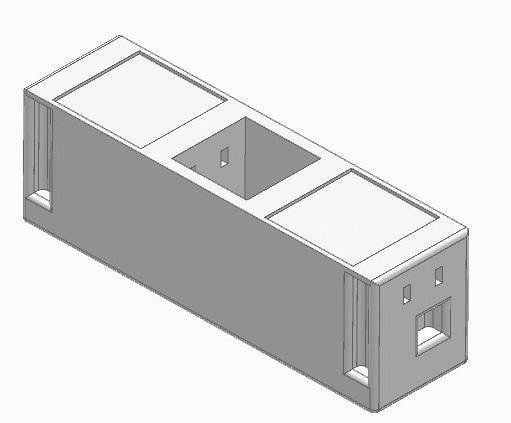
\includegraphics[width=0.7\textwidth]{img/SuperiorReal_simplificado_vista.jpg}
        \caption{\textit{Vista del soporte superior mostrando la configuración estructural, alojamientos de varillas y zonas de montaje.}}
        \label{fig:SuperiorReal_simplificado_vista}
    \end{subfigure}
    \hspace{0.5cm}
    \begin{subfigure}{0.35\textwidth}
        \centering
        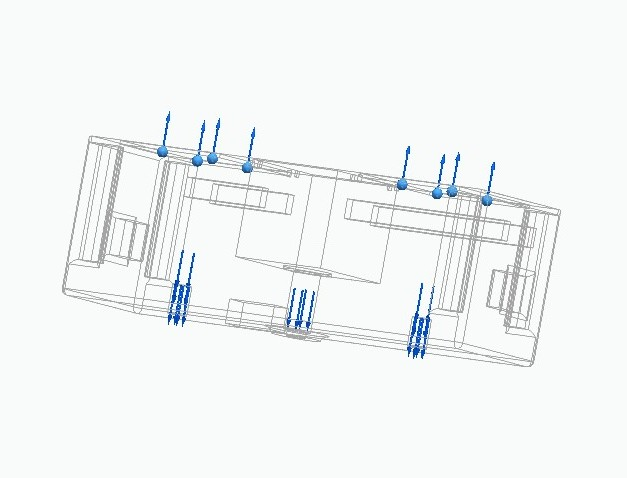
\includegraphics[width=0.7\textwidth]{img/SuperiorReal_simplificado_fuerzas_app.jpg}
        \caption{\textit{Distribución de cargas aplicadas sobre el soporte superior.}}
        \label{fig:SuperiorReal_simplificado_fuerzas_app}
    \end{subfigure}
    \caption{\textit{Soporte superior.}}
\end{figure}

El análisis de esfuerzos mediante elementos finitos se realizó considerando material PLA con las siguientes propiedades mecánicas:

\begin{itemize}[label=$\bullet$]
    \item Módulo de Young: 3500 MPa
    \item Límite de fluencia: 50 MPa
    \item Coeficiente de Poisson: 0.36
\end{itemize}

La Figura \ref{fig:SuperiorReal_simplificado_tensiones} presenta los resultados del análisis, mostrando las deformaciones resultantes. Los resultados indican:

\begin{itemize}[label=$\bullet$]
    \item Deformación máxima: $\approx$ 0.15 mm (en zonas de mayor voladizo)
    \item Factor de seguridad: $\frac{50\,\text{MPa}}{2.8\,\text{MPa}} \approx 18$ (ampliamente seguro)
\end{itemize}

\begin{figure}[H]
    \centering
    \begin{subfigure}{0.48\textwidth}
        \centering
    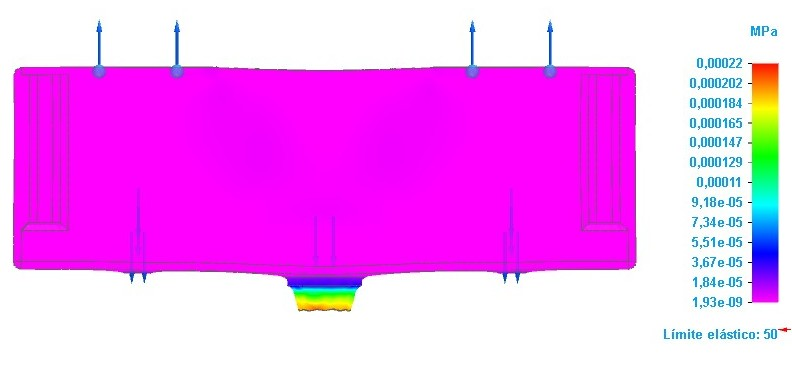
\includegraphics[width=0.78\textwidth]{img/tensiones_Real.jpg}
    \caption{Distribución de tensiones en el soporte superior bajo carga máxima.}
    \label{fig:tensiones_Real}
    \end{subfigure}
    \hspace{0.5cm}
    \begin{subfigure}{0.48\textwidth}
        \centering
    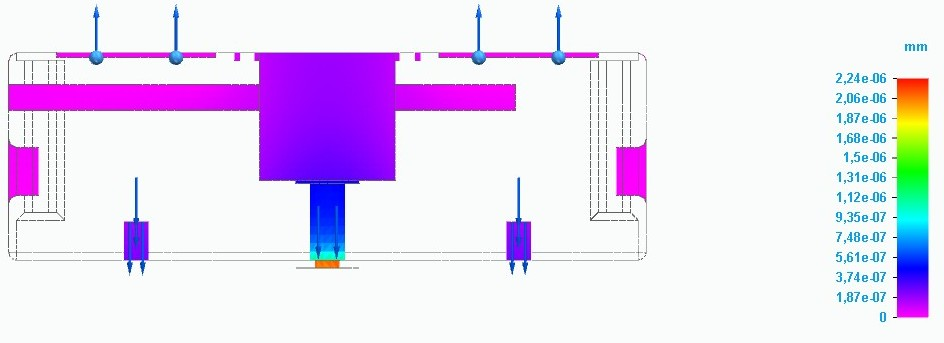
\includegraphics[width=0.9\textwidth]{img/SuperiorReal_simplificado_tensiones.jpg}
    \caption{Distribución de deformaciones en el soporte superior bajo carga máxima.}
    \label{fig:SuperiorReal_simplificado_tensiones}
    \end{subfigure}
    \caption{\textit{Tensiones y deformaciones del soporte superior.}}
\end{figure}
Los resultados confirman que el diseño propuesto es estructuralmente robusto, con tensiones muy por debajo del límite de fluencia del material y deformaciones despreciables para los requerimientos operacionales del sistema.

\subsubsection{Soporte medio}

El soporte medio constituye el elemento móvil del eje vertical, desplazándose a lo largo de las varillas mediante el giro de la varilla roscada. Este componente cumple funciones críticas en el sistema: montaje del brazo robótico serial, fijación de la cámara de visión artificial y mantenimiento del equilibrio dinámico mediante contrapeso.

\begin{itemize}[label=$\bullet$]
    \item \underline{Sistema de guiado:} Incorpora dos rodamientos lineales LM16UU para deslizamiento sobre las varillas lisas de 8 mm, garantizando movimiento suave sin rotaciones indeseadas
    \item \underline{Tuerca de transmisión:} Alojamiento central para tuerca TR16 que se acopla con la varilla roscada, convirtiendo el movimiento rotacional del motor en desplazamiento lineal
    \item \underline{Montaje del brazo:} Base horizontal plana con patrón de agujeros para fijación del servomotor base del brazo robótico
    \item \underline{Montaje de cámara:} Soporte superior para la cámara con ajuste angular para optimización del campo de visión
    \item \underline{Sistema de balanceo:} Contrapeso en el lado opuesto al brazo para reducir momentos flectores sobre las varillas y mejorar la estabilidad dinámica del sistema
\end{itemize}

\begin{figure}[H]
    \centering
    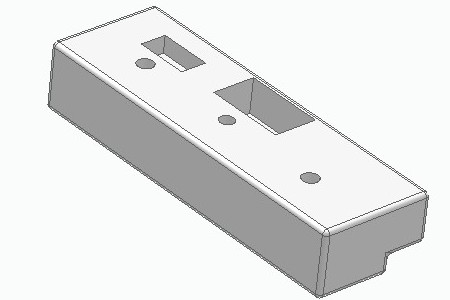
\includegraphics[width=0.5\textwidth]{img/MedioReal_simplificado_vista.jpg}
    \caption{Vista general del soporte medio mostrando el montaje del brazo robótico, alojamiento de la cámara, sistema de guiado lineal y contrapeso de equilibrio.}
    \label{fig:soporte_medio_Real}
\end{figure}

El contrapeso permite compensar el momento generado por el brazo extendido, reduciendo las cargas laterales sobre las guías lineales y mejorando la precisión de posicionamiento vertical. El diseño modular facilita el reemplazo del brazo o la cámara sin necesidad de rediseñar el soporte completo.

\subsubsection{Soporte inferior}

El soporte inferior cierra la estructura vertical del sistema, proporcionando la base de fijación para los extremos inferiores de las tres varillas y alojando componentes auxiliares del sistema de control.\\

Funciones y características

\begin{itemize}[label=$\bullet$]
    \item \underline{Anclaje de varillas:} Alojamientos pasantes para las dos varillas lisas con fijación mediante tornillos prisioneros, y soporte del extremo libre de la varilla roscada con rodamiento axial
    \item \underline{Final de carrera inferior:} Montaje del microswitch de límite inferior del eje vertical, con placa de activación mecánica
\end{itemize}

\begin{figure}[H]
    \centering
    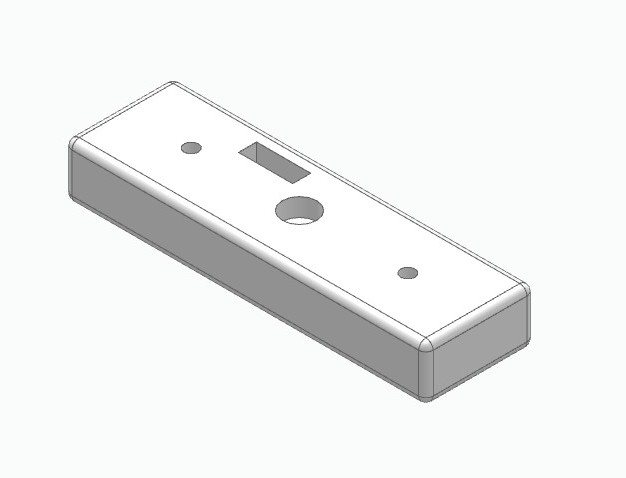
\includegraphics[width=0.5\textwidth]{img/InferiorReal_simplificado_vista.jpg}
    \caption{\textit{Soporte inferior, se muestra el alojamiento del final de carrera inferior.}}
    \label{fig:soporte_inferior_real}
\end{figure}

El diseño incorpora tolerancias ajustadas para los alojamientos de las varillas, garantizando la perpendicularidad del eje vertical respecto al plano horizontal de desplazamiento.

\subsubsection{Brazo robótico serie}

Se opta por el uso de PLA con fibra de carbono como material estructural proporciona mejor relación rigidez/peso que el PLA estándar, reduciendo las vibraciones residuales al finalizar movimientos rápidos y mejorando la precisión de posicionamiento del efector final.

\begin{figure}[H]
    \centering
    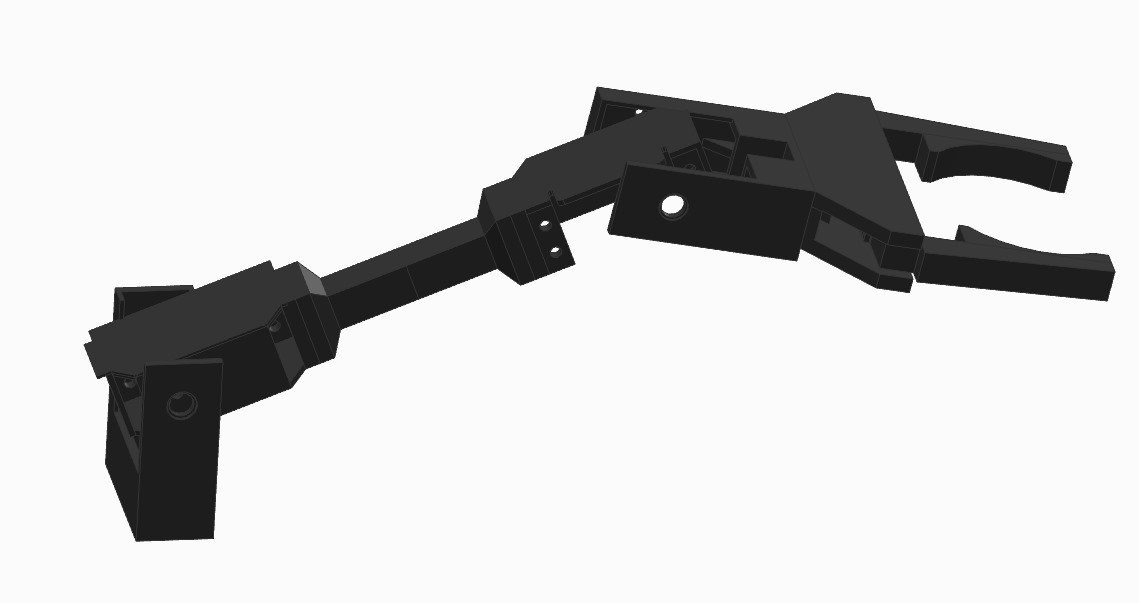
\includegraphics[width=0.5\textwidth]{img/brazo_completo.jpg}
    \caption{\textit{Vista completa del brazo robótico de 2 grados de libertad mostrando las dos articulaciones rotacionales y el efector final tipo pinza.}}
    \label{fig:brazo_Real}
\end{figure}

\subsubsection{Efector final}

El efector final implementa un mecanismo de pinza paralela actuado mediante transmisión piñón-cremallera, convirtiendo el movimiento rotacional del servomotor en desplazamiento lineal de las mordazas.\\

Principio de funcionamiento

\begin{itemize}[label=$\bullet$]
    \item \underline{Transmisión:} Sistema piñón-cremallera con relación 1:1, proporcionando movimiento sincronizado de ambas mordazas hacia el centro
    \item \underline{Rango de apertura:} 0-50 mm, adecuado para lechugas de tamaño pequeño a grande
    \item \underline{Mordazas:} Geometría curva con superficie texturizada para mejorar fricción sin penetrar las hojas
\end{itemize}

\begin{figure}[H]
    \centering
    \begin{subfigure}{0.35\textwidth}
        \centering
        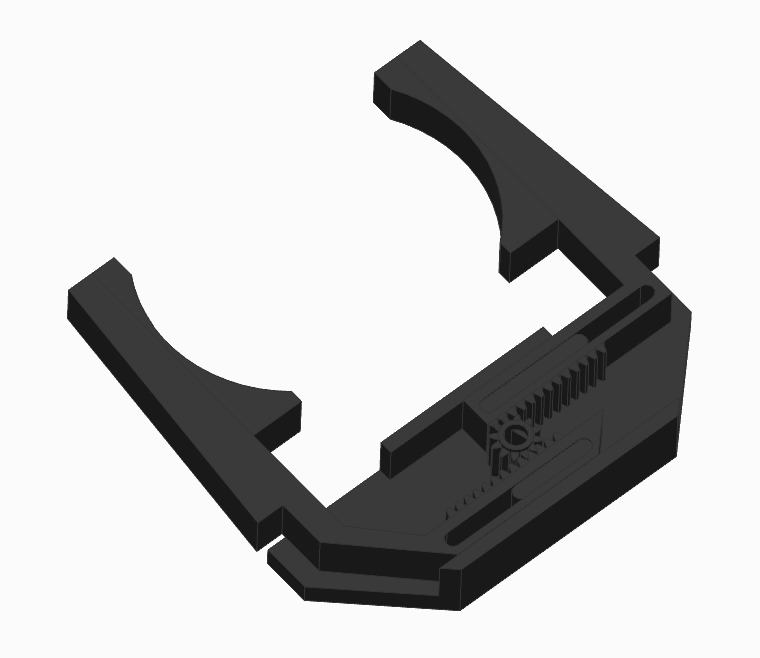
\includegraphics[width=0.7\textwidth]{img/gripper.jpg}
        \caption{\textit{Sistema de transmisión piñón-cremallera del gripper mostrando el acoplamiento mecánico entre el servomotor y las mordazas móviles.}}
        \label{fig:gripper_Real_transmision}
    \end{subfigure}
    \hspace{0.5cm}
    \begin{subfigure}{0.35\textwidth}
        \centering
        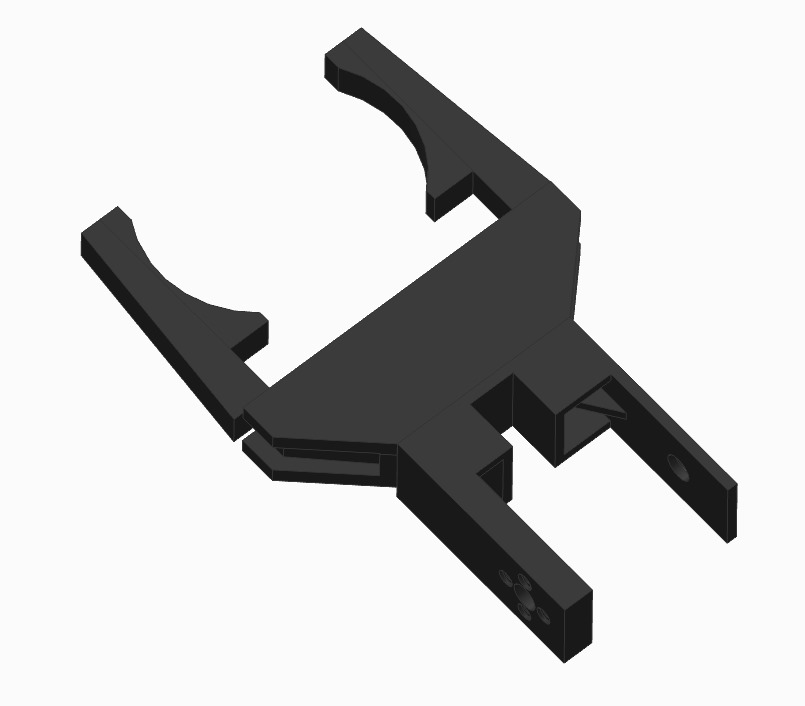
\includegraphics[width=0.7\textwidth]{img/pinza_tapa.png}
        \caption{\textit{Vista del gripper ensamblado mostrando la configuración de mordazas paralelas y carcasa de protección.}}
        \label{fig:gripper_Real}
    \end{subfigure}
    \caption{\textit{Efector final tipo gripper con transmisión por piñón-cremallera para agarre de lechugas.}}
\end{figure}


%% Tolerancias Ajustes



\section{Selección de hardware y análisis energético}
La implementación del sistema robótico de cosecha requiere la selección de componentes electrónicos que satisfagan los requerimientos funcionales de control, procesamiento y actuación. Este apartado presenta la justificación de los componentes seleccionados y el análisis energético del sistema completo.

Los criterios de selección priorizaron disponibilidad comercial en el mercado local, relación costo-beneficio, compatibilidad entre componentes, y capacidad de procesamiento adecuada para las tareas requeridas.

\subsection{Drivers de potencia}
El control del motor paso a paso NEMA 17 long se realiza mediante el driver TB6600, que proporcionan control de corriente mediante chopper y aislamiento óptico de señales lógicas. El driver opera con 24V DC para los motores, y tensión lógica de 5V DC para las señales STEP/DIR/ENABLE, además Este driver tiene consumo máximo de 3 A a 24V cuando el motor está energizado y girando a máxima velocidad. En reposo (motor energizado pero detenido), el consumo se reduce a 1 A por driver. 

%Los motores NEMA 17 especificados tienen corriente nominal de 1.5 A por fase. Los drivers se configuran mediante DIP switches para limitar la corriente a 1.5 A, protegiendo los motores ante sobrecarga térmica.
Dicho motor posee corriente nominal de 1.8 A por fase, mientras que el driver puede entregar hasta 3.5A de corriente de control.

Por otro lado, el control del motor Nema 34 medium se realiza mediante el driver KTC-DM860H-0 que se alimenta con 24V y entrega una corriente de control máxima de 7.2A. El consumo es de 6A cuando el motor está energizado y girando a máxima velocidad y de 2.5A cuando el motor está en reposo.

Los drivers se configuran mediante DIP switches para limitar la corriente a 1.8 A, o 4.5A segun el caso, protegiendo los motores ante sobrecarga térmica.

\subsection{Cámara USB de visión}

Se implementó una cámara USB 3.0 con sensor de 2 MP, lente ojo de pez y sensor Sony IMX291. Las características principales son:

\textbf{Resolución.} El sensor proporciona imágenes de 1920×1080 píxeles (Full HD), resolución suficiente para detectar lechugas de 8-12 cm de diámetro a distancias de 15-25 cm con al menos 120 píxeles de ancho, permitiendo clasificación confiable por área.

\textbf{Lente ojo de pez.} La distorsión radial del lente gran angular proporciona campo de visión amplio (aproximadamente 120°) a distancias cortas, permitiendo capturar el área completa de una estación de cultivo (15×15 cm) desde 20 cm de distancia. Aunque introduce distorsión geométrica, el clasificador morfológico es robusto ante estas deformaciones dado que opera sobre área de contornos en píxeles.

\textbf{Sensibilidad.} El sensor Sony IMX291 presenta sensibilidad adecuada para las condiciones de iluminación del invernadero (200-800 lux), con rango dinámico suficiente para manejar variaciones de luz natural.

\textbf{Interfaz USB 3.0.} La conectividad USB 3.0 proporciona ancho de banda de hasta 5 Gbps, suficiente para transmitir video Full HD a 30 fps sin compresión. El protocolo USB garantiza robustez ante interferencia electromagnética generada por motores y drivers.

El consumo de la cámara es de aproximadamente 500 mA a 5V (2.5 W) durante captura continua de video.

\subsection{Microcontrolador: Arduino Mega 2560}

El controlador de bajo nivel seleccionado es un Arduino Mega 2560 basado en el microcontrolador ATmega2560, que opera a 16 MHz con arquitectura de 8 bits. La selección se fundamenta en los siguientes criterios técnicos:

Los drivers TB6600 seleccionados requieren señales lógicas de 5V para las entradas STEP, DIR y ENABLE. El Arduino Mega 2560 proporciona salidas digitales de 5V nativas, asegurando compatibilidad directa sin necesidad de circuitos de adaptación de nivel lógico. 

El Arduino Mega proporciona 54 pines digitales (de los cuales 15 soportan PWM) y 16 entradas analógicas, superando ampliamente los 17 pines digitales requeridos.

La generación de perfiles de velocidad trapezoidales requiere interrupciones de alta frecuencia (hasta 15 kHz) para emisión de pulsos STEP con precisión temporal. El ATmega2560 incorpora 6 timers hardware (cuatro de 8 bits y dos de 16 bits) que permiten generar señales PWM y manejar interrupciones sin sobrecarga del procesador principal.

El microcontrolador dispone de 4 puertos UART hardware, permitiendo comunicación con el nivel supervisor a 115200 baudios sin consumo de ciclos de CPU para manejo de protocolo.

El Arduino Mega 2560 opera a 5V DC con consumo típico de 200 mA durante operación normal, alcanzando picos de 500 mA durante conmutación simultánea de múltiples salidas digitales.
\subsection{Microcomputador: Raspberry Pi 5}

El nivel supervisor se implementa sobre una Raspberry Pi 5 con procesador ARM Cortex-A76 quad-core a 2.4 GHz y 8 GB de memoria RAM LPDDR4X. La selección se justifica por:

La cámara seleccionada requiere interfaz USB 3.0 para transmitir video Full HD . La Raspberry Pi 5 incorpora 2 puertos USB 3.0 nativos que proporcionan hasta 5 Gbps por puerto, garantizando ancho de banda suficiente para captura de imágenes de alta resolución en tiempo real. El sistema operativo Raspberry Pi OS proporciona soporte nativo para el controlador V4L2 (Video4Linux2), permitiendo integración directa con bibliotecas de procesamiento de imágenes sin desarrollo de drivers adicionales.

Los algoritmos de visión por computadora requieren operaciones matriciales intensivas sobre imágenes de 1920×1080 píxeles. El procesador quad-core a 2.4 GHz permite ejecutar el proceso completo de clasificación en tiempo real.

 Python 3.11 con bibliotecas científicas maduras (NumPy, OpenCV, PySerial) permite desarrollo ágil de algoritmos de visión. La compatibilidad con OpenCV 4.x está completamente validada en la plataforma, simplificando la implementación de pipelines de procesamiento de imágenes. El sistema operativo Linux proporciona capacidades multitarea para ejecución concurrente de procesos de control, visión, y comunicación.

La Raspberry Pi 5 opera a 5V DC mediante conector USB-C, con consumo típico de 3 A (15 W) durante procesamiento intensivo de imágenes, y mínimo de 1 A (5 W) en estado idle.

\subsection{Reguladores de voltaje}

El sistema emplea dos reguladores DC-DC step-down para adaptar la tensión de alimentación principal (24V DC) a los niveles requeridos por diferentes subsistemas:

\underline{Regulador 24V - 5V:} Regulador conmutado step-down con capacidad de 5 A. Este regulador alimenta:
\begin{itemize}[label=$\bullet$]
\item Arduino Mega 2560 (consumo típico 0.5 A)
\item Raspberry Pi 5 (consumo típico 3 A, picos de 4 A)
\item Cámara USB (consumo 0.5 A)
\item Margen de seguridad: 1 A adicional
\end{itemize}

La capacidad total requerida es de 5 A, considerando operación simultánea de todos los dispositivos a carga máxima. El regulador seleccionado proporciona exactamente esta capacidad con margen de seguridad del 20\%.

\underline{Regulador 24V - 7V:} Regulador conmutado step-down con capacidad de 5 A. Este regulador alimenta los servo motores. Cada driver consume aproximadamente 100 mA en su circuito lógico, resultando en consumo total de 300 mA.

La separación de la alimentación lógica de los drivers respecto a la alimentación de procesadores (5V) previene caídas de tensión causadas por conmutación de alta frecuencia que podrían inducir resets espurios del Arduino.

La Figura \ref{fig:diagrama_voltajes} ilustra el esquema completo de distribución de voltajes desde la fuente primaria de 24V hasta todos los componentes del sistema.

\begin{figure}[H]
\centering
% TODO: Agregar imagen del diagrama de distribución de voltajes
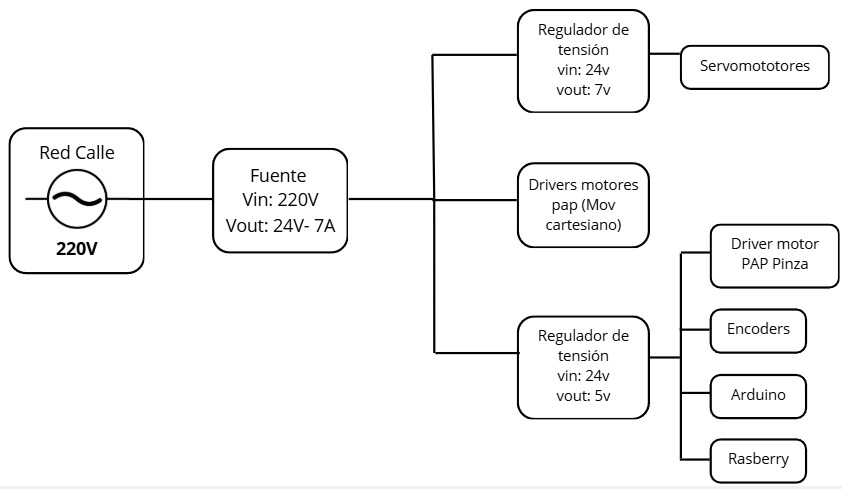
\includegraphics[width=0.75\textwidth]{imagenes/diagrama_voltajes.jpg}
\caption{\textit{Diagrama de distribución de voltajes del sistema mostrando fuente de 24V, reguladores step-down (24V→5V y 24V→7V), y conexiones a todos los componentes}}
\label{fig:diagrama_voltajes}
\end{figure}

\subsection{Análisis energético y dimensionamiento de fuente}

La Tabla \ref{tab:consumo_energetico} presenta el consumo eléctrico de cada componente del sistema en diferentes estados operativos.

\begin{table}[H]
\centering
\small
\begin{tabular}{|l|c|c|c|c|}
\hline
\textbf{Componente} & \textbf{Voltaje} & \textbf{Reposo (A)} & \textbf{Operación (A)} & \textbf{Pico (A)} \\
\hline
\multicolumn{5}{|c|}{\textbf{Alimentación 24V}} \\
\hline
Driver TB6600 ($\times$2, NEMA 17) & 24V & 2.0 & 6.0 & 6.0 \\
\hline
Driver KTC-DM860H-0 ($\times$1, NEMA 34) & 24V & 2.5 & 6.0 & 6.0 \\
\hline
Regulador 24V$\rightarrow$5V (5A)& 24V & 0.35 & 0.89 & 1.16 \\
\hline
Regulador 24V$\rightarrow$12V (10A)& 24V & 0.17 & 5.5 & 5.5 \\
\hline
\multicolumn{2}{|l|}{\textbf{Subtotal 24V}} & \textbf{5.02} & \textbf{18.39} & \textbf{18.66} \\
\hline
\hline
\multicolumn{5}{|c|}{\textbf{Alimentación 5V (desde regulador 24V$\rightarrow$5V)}} \\
\hline
Arduino Mega 2560 & 5V & 0.2 & 0.35 & 0.5 \\
\hline
Raspberry Pi 5 & 5V & 1.0 & 3.0 & 4.0 \\
\hline
Cámara USB & 5V & 0.3 & 0.5 & 0.5 \\
\hline
\multicolumn{2}{|l|}{\textbf{Subtotal 5V}} & \textbf{1.5} & \textbf{3.85} & \textbf{5.0} \\
\hline
\hline
\multicolumn{5}{|c|}{\textbf{Alimentación 12V (desde regulador 24V$\rightarrow$12V)}} \\
\hline
Servomotores Dynamixel MX-106T/R ($\times$2) & 12V & 0.0 & 9.6 & 9.6 \\
\hline
Lógica drivers ($\times$3) & 12V & 0.3 & 0.3 & 0.3 \\
\hline
\multicolumn{2}{|l|}{\textbf{Subtotal 12V}} & \textbf{0.3} & \textbf{9.9} & \textbf{9.9} \\
\hline
\hline
\multicolumn{5}{|c|}{\textbf{Consumo total en fuente de 24V}} \\
\hline
\multicolumn{2}{|l|}{Idle} & \multicolumn{3}{c|}{5.02 A @ 24V = \textbf{120 W}} \\
\hline
\multicolumn{2}{|l|}{Operación normal} & \multicolumn{3}{c|}{18.39 A @ 24V = \textbf{441 W}} \\
\hline
\multicolumn{2}{|l|}{Pico máximo} & \multicolumn{3}{c|}{18.66 A @ 24V = \textbf{448 W}} \\
\hline
\end{tabular}
\caption{\textit{Consumo eléctrico del sistema por componente y estado operativo}}
\label{tab:consumo_energetico}
\end{table}
%\footnotetext[1]{Consumo calculado considerando eficiencia del 90\% según carga real en cada estado}

El consumo en operación normal (441 W) ocurre cuando los motores paso a paso están en movimiento continuo, los servomotores Dynamixel operan bajo carga, y el sistema de visión está procesando imágenes simultáneamente. Los picos de 448 W ocurren durante aceleraciones bruscas con los tres motores paso a paso y los dos servomotores iniciando movimiento simultáneamente.

Se selecciona una fuente conmutada de 24V DC con capacidad nominal de 20 A (480 W), proporcionando un margen de seguridad del 7.1\% sobre el pico máximo calculado. Este margen considera:

\begin{itemize}[label=$\bullet$]
\item Degradación de la fuente con el tiempo (típicamente 10-15\% de pérdida de capacidad tras 2 años de operación continua)
\item Transitorios de corriente durante arranque inicial del sistema
\item Posibles expansiones futuras del hardware (sensores adicionales, iluminación LED, etc.)
\end{itemize}

La eficiencia de los reguladores step-down (90\% para 24V$\rightarrow$5V y 90\% para 24V$\rightarrow$12V) ya está considerada en los cálculos de consumo de la fuente primaria. Las pérdidas totales por conversión de voltaje son de aproximadamente 15.3 W en operación normal (2.1 W en el regulador 24V$\rightarrow$5V y 13.2 W en el regulador 24V$\rightarrow$12V).


\section{Sistema de control de bajo nivel (nivel regulatorio)}

\subsection{Arquitectura del nivel regulatorio}
El nivel regulatorio constituye el sistema de control en tiempo real del robot, gestionando directamente actuadores y sensores mediante ejecución de comandos recibidos desde el nivel supervisor.

El firmware se estructura en tres capas jerárquicas que separan responsabilidades según nivel de abstracción, como se muestra en la Figura \ref{fig:arquitectura_regulatorio}:

\begin{itemize}[label=$\bullet$]
\item \textbf{Capa de controladores de hardware (drivers):} Interactúa directamente con periféricos del microcontrolador mediante registros y temporizadores
\item \textbf{Capa de control de movimiento:} Implementa generación de trayectorias mediante perfiles de velocidad y coordinación de ejes
\item \textbf{Capa de aplicación:} Proporciona interfaz de alto nivel para comandos del sistema supervisor mediante protocolo UART
\end{itemize}

\begin{figure}[H]
    \centering
    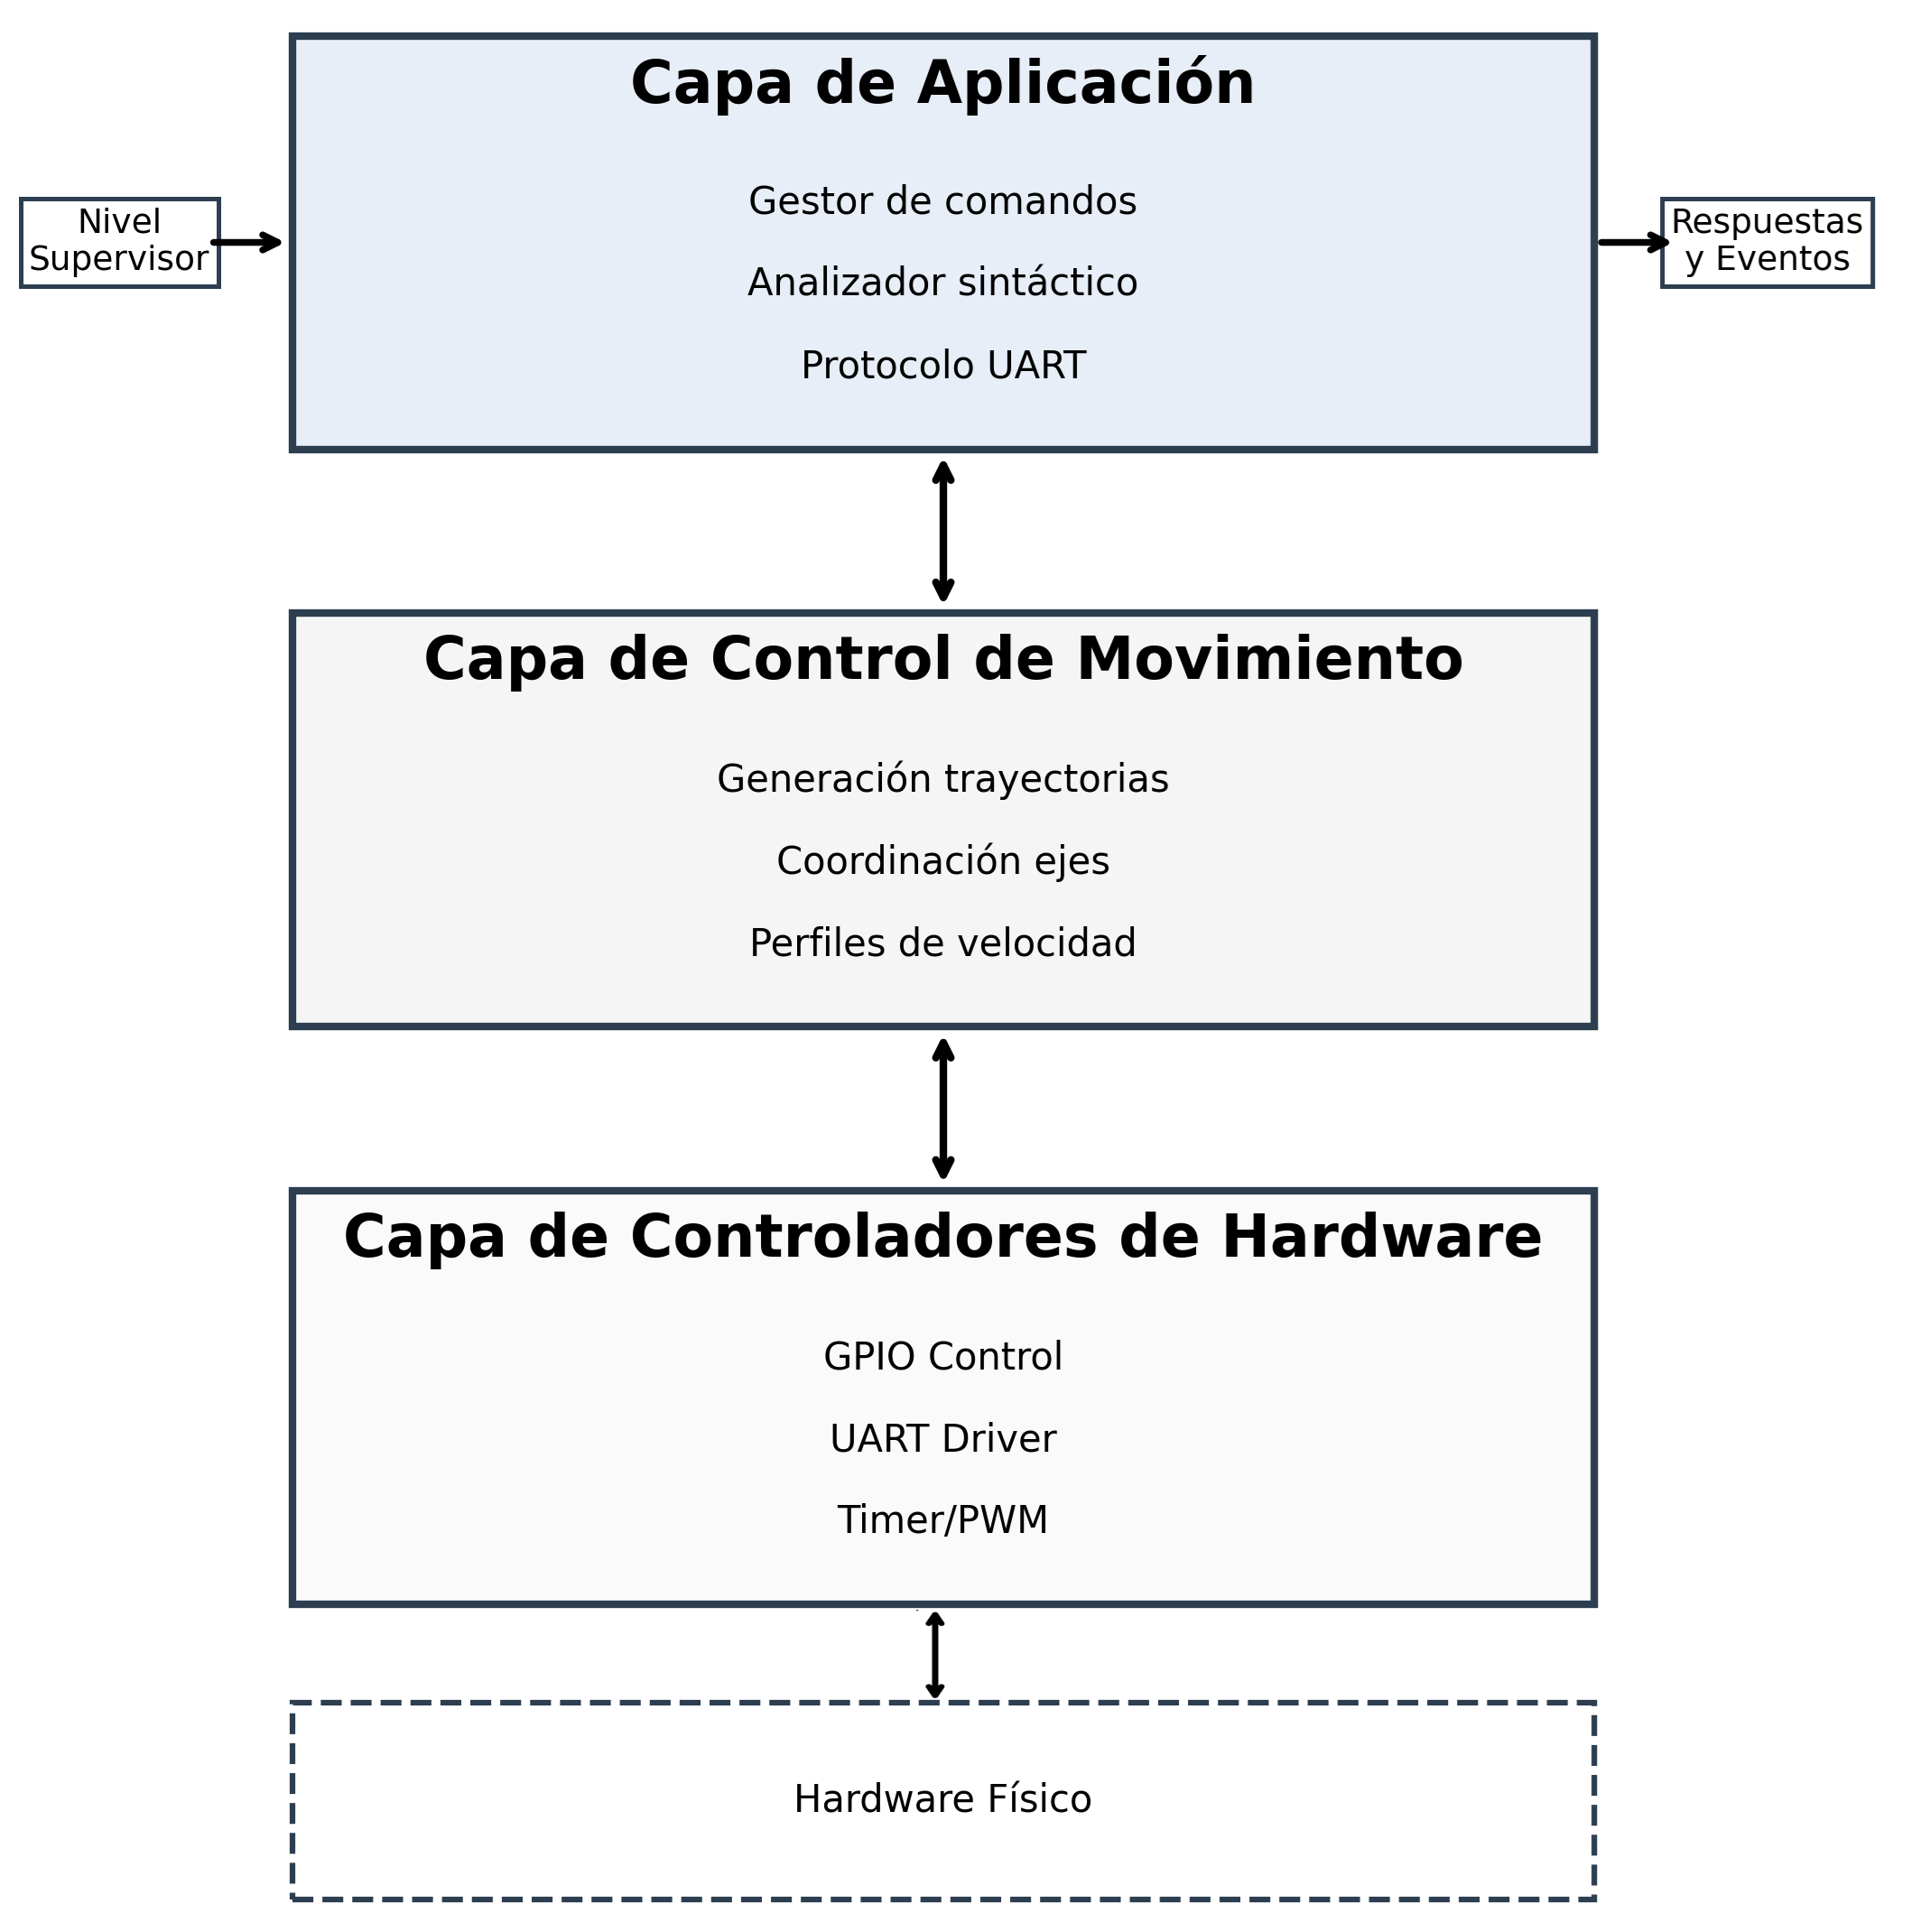
\includegraphics[width=0.7\textwidth]{imagenes/arquitectura_regulatorio_capas.png}
    \caption{\textit{Arquitectura en capas del firmware del nivel regulatorio}}
    \label{fig:arquitectura_regulatorio}
\end{figure}


% \subsection{Selección y Dimensionamiento de Actuadores}
% % Motores Paso Paso


% % Drivers Tb6600


% % Servomotores



% \subsection{Sensores de Seguridad}
% % Finales Carrera


% % Sistema Seguridad



\subsection{Generación de trayectorias y control de movimiento}
\subsubsection{Perfiles de Velocidad para Control de Movimiento}

El sistema implementa perfiles de velocidad trapezoidales con aceleraciones fijas, garantizando comportamiento predecible independientemente de la distancia del movimiento. Las distancias de aceleración y desaceleración permanecen constantes, variando únicamente la longitud de la zona de crucero.

Para movimientos largos (superiores a 25mm), el perfil se compone de las fases mostradas en la Tabla \ref{tab:perfil_trapezoidal}. Esta estrategia asegura que las aceleraciones sean idénticas para todos los movimientos, proporcionando comportamiento mecánico consistente. Por ejemplo, un movimiento de 25mm tiene 12.5mm de aceleración/desaceleración y 12.5mm de crucero, mientras que un movimiento de 250mm mantiene los mismos 12.5mm de aceleración/desaceleración pero dispone de 237.5mm de crucero.

\begin{table}[H]
\centering
\small
\begin{tabular}{|l|c|c|c|c|}
\hline
\textbf{Fase} & \textbf{Distancia} & \textbf{$v_i$} & \textbf{$v_f$} & \textbf{Aceleración} \\
\hline
1. Arranque & Instant. & 0 & 0.05 & - \\
\hline
2. Acel. suave & 5 mm & 0.05 & 0.10 & 0.05 m/s² \\
\hline
3. Acel. fuerte & 7.5 mm & 0.10 & 0.375 (H) / 0.30 (V) & 0.37 / 0.27 m/s² \\
\hline
4. Crucero & Variable & 0.375 / 0.30 & 0.375 / 0.30 & 0 \\
\hline
5. Decel. fuerte & 7.5 mm & 0.375 / 0.30 & 0.10 & -0.37 / -0.27 m/s² \\
\hline
6. Decel. suave & 5 mm & 0.10 & 0.05 & -0.05 m/s² \\
\hline
7. Detención & Instant. & 0.05 & 0 & - \\
\hline
\end{tabular}
\caption{Fases del perfil trapezoidal de velocidad con aceleraciones fijas. Velocidades en m/s, H: horizontal, V: vertical}
\label{tab:perfil_trapezoidal}
\end{table}

\begin{figure}[H]
    \centering
    % TODO: Insertar gráfico comparativo mostrando mismo perfil de aceleración para diferentes distancias
    % Mostrar: dos movimientos (25mm vs 250mm) con mismas rampas de accel/decel pero diferente zona crucero
    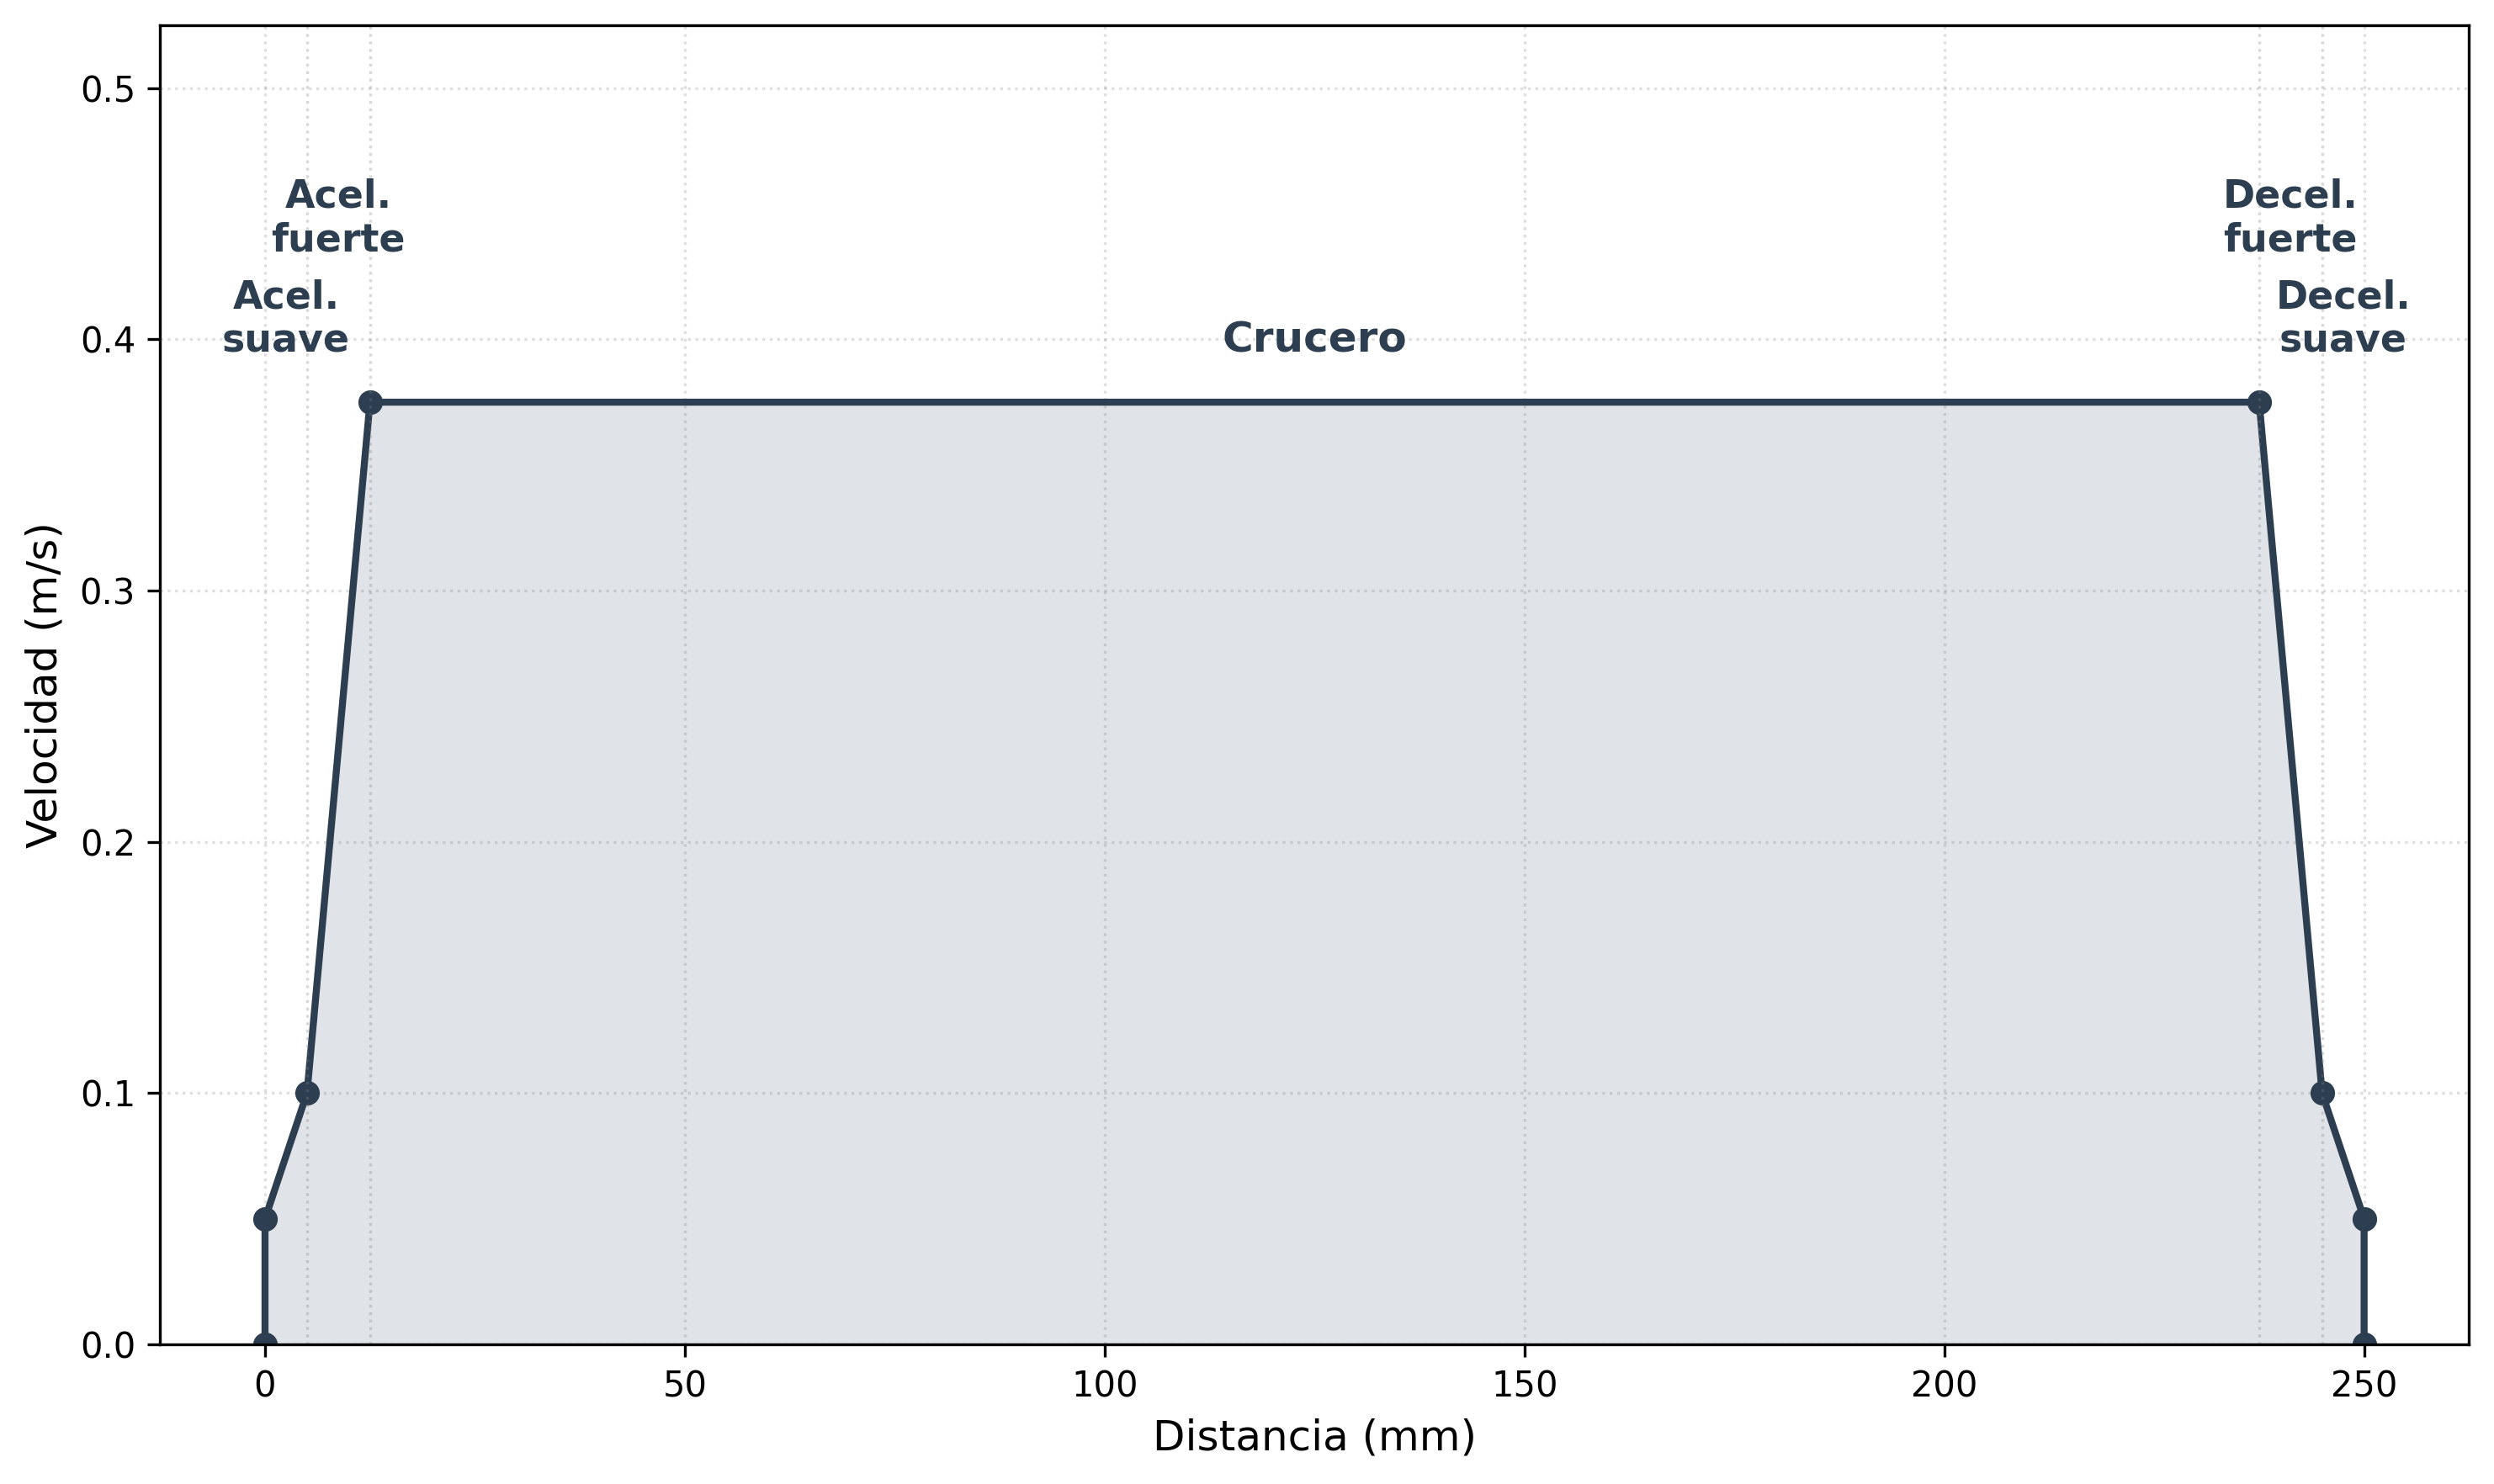
\includegraphics[width=0.7\textwidth]{imagenes/perfil_trapezoidal_velocidad.png}
    \caption{Perfil trapezoidal con aceleraciones fijas. Las zonas de aceleración y desaceleración mantienen longitud constante (12.5mm cada una), mientras que la zona de crucero se ajusta según la distancia total}
    \label{fig:perfil_trapezoidal}
\end{figure}

Cuando la distancia total es menor que 25mm (suma de las zonas de aceleración y desaceleración), el perfil se convierte en triangular. El sistema mantiene las mismas aceleraciones de la Tabla \ref{tab:perfil_trapezoidal}, pero calcula el punto medio del movimiento donde debe iniciar la desaceleración para alcanzar exactamente la posición final. En este caso, la velocidad máxima alcanzada es menor que la velocidad de crucero nominal, ya que el motor comienza a frenar antes de alcanzarla. Por ejemplo, un movimiento de 10mm acelera durante 5mm hasta alcanzar aproximadamente 0.15 m/s, y luego desacelera durante los siguientes 5mm hasta detenerse (Figura \ref{fig:perfil_comparacion}).

Para movimientos muy cortos (menos de 2.5mm), el sistema reduce la velocidad máxima permitida a 0.10 m/s para mantener precisión en el posicionamiento final, típico en operaciones de ajuste fino.

\begin{figure}[H]
    \centering
    % TODO: Insertar gráfico comparativo: perfil trapezoidal vs triangular
    % Mostrar: movimiento largo con zona crucero vs movimiento corto sin zona crucero (triangular)
    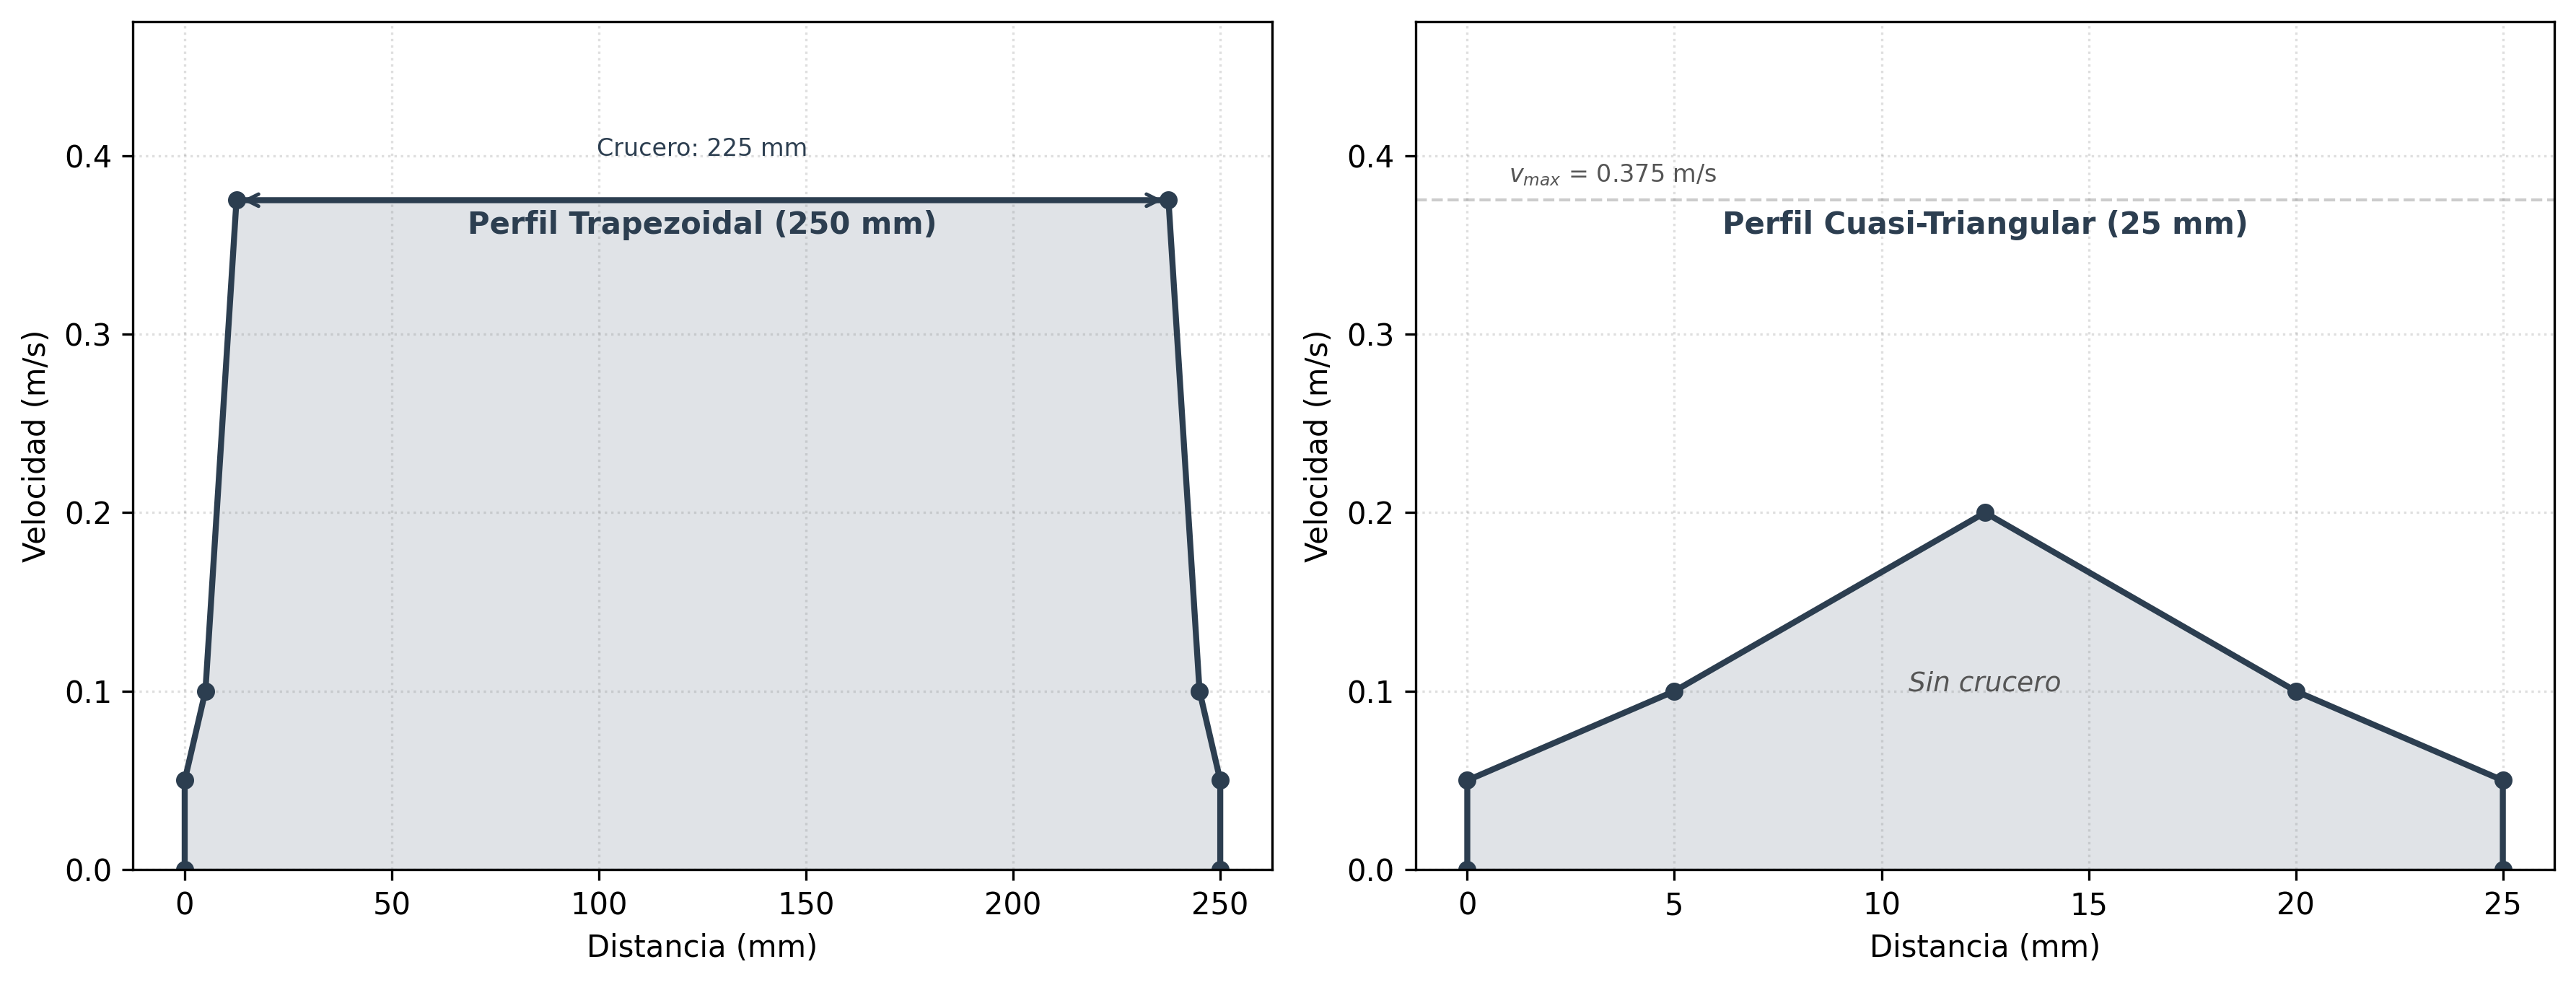
\includegraphics[width=0.7\textwidth]{imagenes/perfil_trapezoidal_triangular.png}
    \caption{Comparación entre perfil trapezoidal (movimientos largos) y triangular (movimientos cortos). Ambos utilizan las mismas aceleraciones, pero el perfil triangular invierte la aceleración en el punto medio}
    \label{fig:perfil_comparacion}
\end{figure}

La velocidad instantánea en cada paso se calcula mediante interpolación lineal dentro de cada zona. El firmware ejecuta este cálculo continuamente en el loop principal a frecuencia superior a 10kHz, actualizando el registro OCR1A del Timer1 que controla la frecuencia de generación de pulsos STEP. La conversión entre velocidad deseada $v$ (en pasos/s) y el valor del registro es:

\begin{equation}
OCR1A = \frac{f_{CPU}}{2 \cdot prescaler \cdot v} - 1 = \frac{1,000,000}{v} - 1
\end{equation}

donde $f_{CPU} = 16$ MHz y prescaler = 8. Por ejemplo, para $v = 5,000$ pasos/s (0.125 m/s), $OCR1A = 199$. El sistema soporta velocidades entre 500 pasos/s (inicio/fin de movimientos) y 15,000 pasos/s (crucero máximo). Velocidades superiores causan jitter excesivo y riesgo de pérdida de pasos.

Para movimientos diagonales que involucran ambos ejes simultáneamente, el firmware sincroniza los perfiles mediante escalamiento proporcional de velocidades. El eje con mayor distancia a recorrer (eje dominante) utiliza su velocidad de crucero nominal, mientras que el eje subordinado escala su velocidad proporcionalmente: $v_{sub} = v_{dom} \times (d_{sub}/d_{dom})$. Este escalamiento se aplica a todas las fases del perfil, garantizando que ambos ejes completen el movimiento en el mismo tiempo y generando trayectorias rectilíneas en el plano XY (Figura \ref{fig:sincronizacion_multieje}). Por ejemplo, para un movimiento de 100mm horizontal y 50mm vertical, el eje horizontal mantiene 0.375 m/s de crucero mientras que el vertical se reduce a 0.1875 m/s, completando ambos en 0.35s.

\begin{figure}[H]
    \centering
    % TODO: Insertar diagrama de sincronización multi-eje
    % Mostrar: dos ejes con diferentes distancias, perfiles escalados, trayectoria rectilínea resultante
    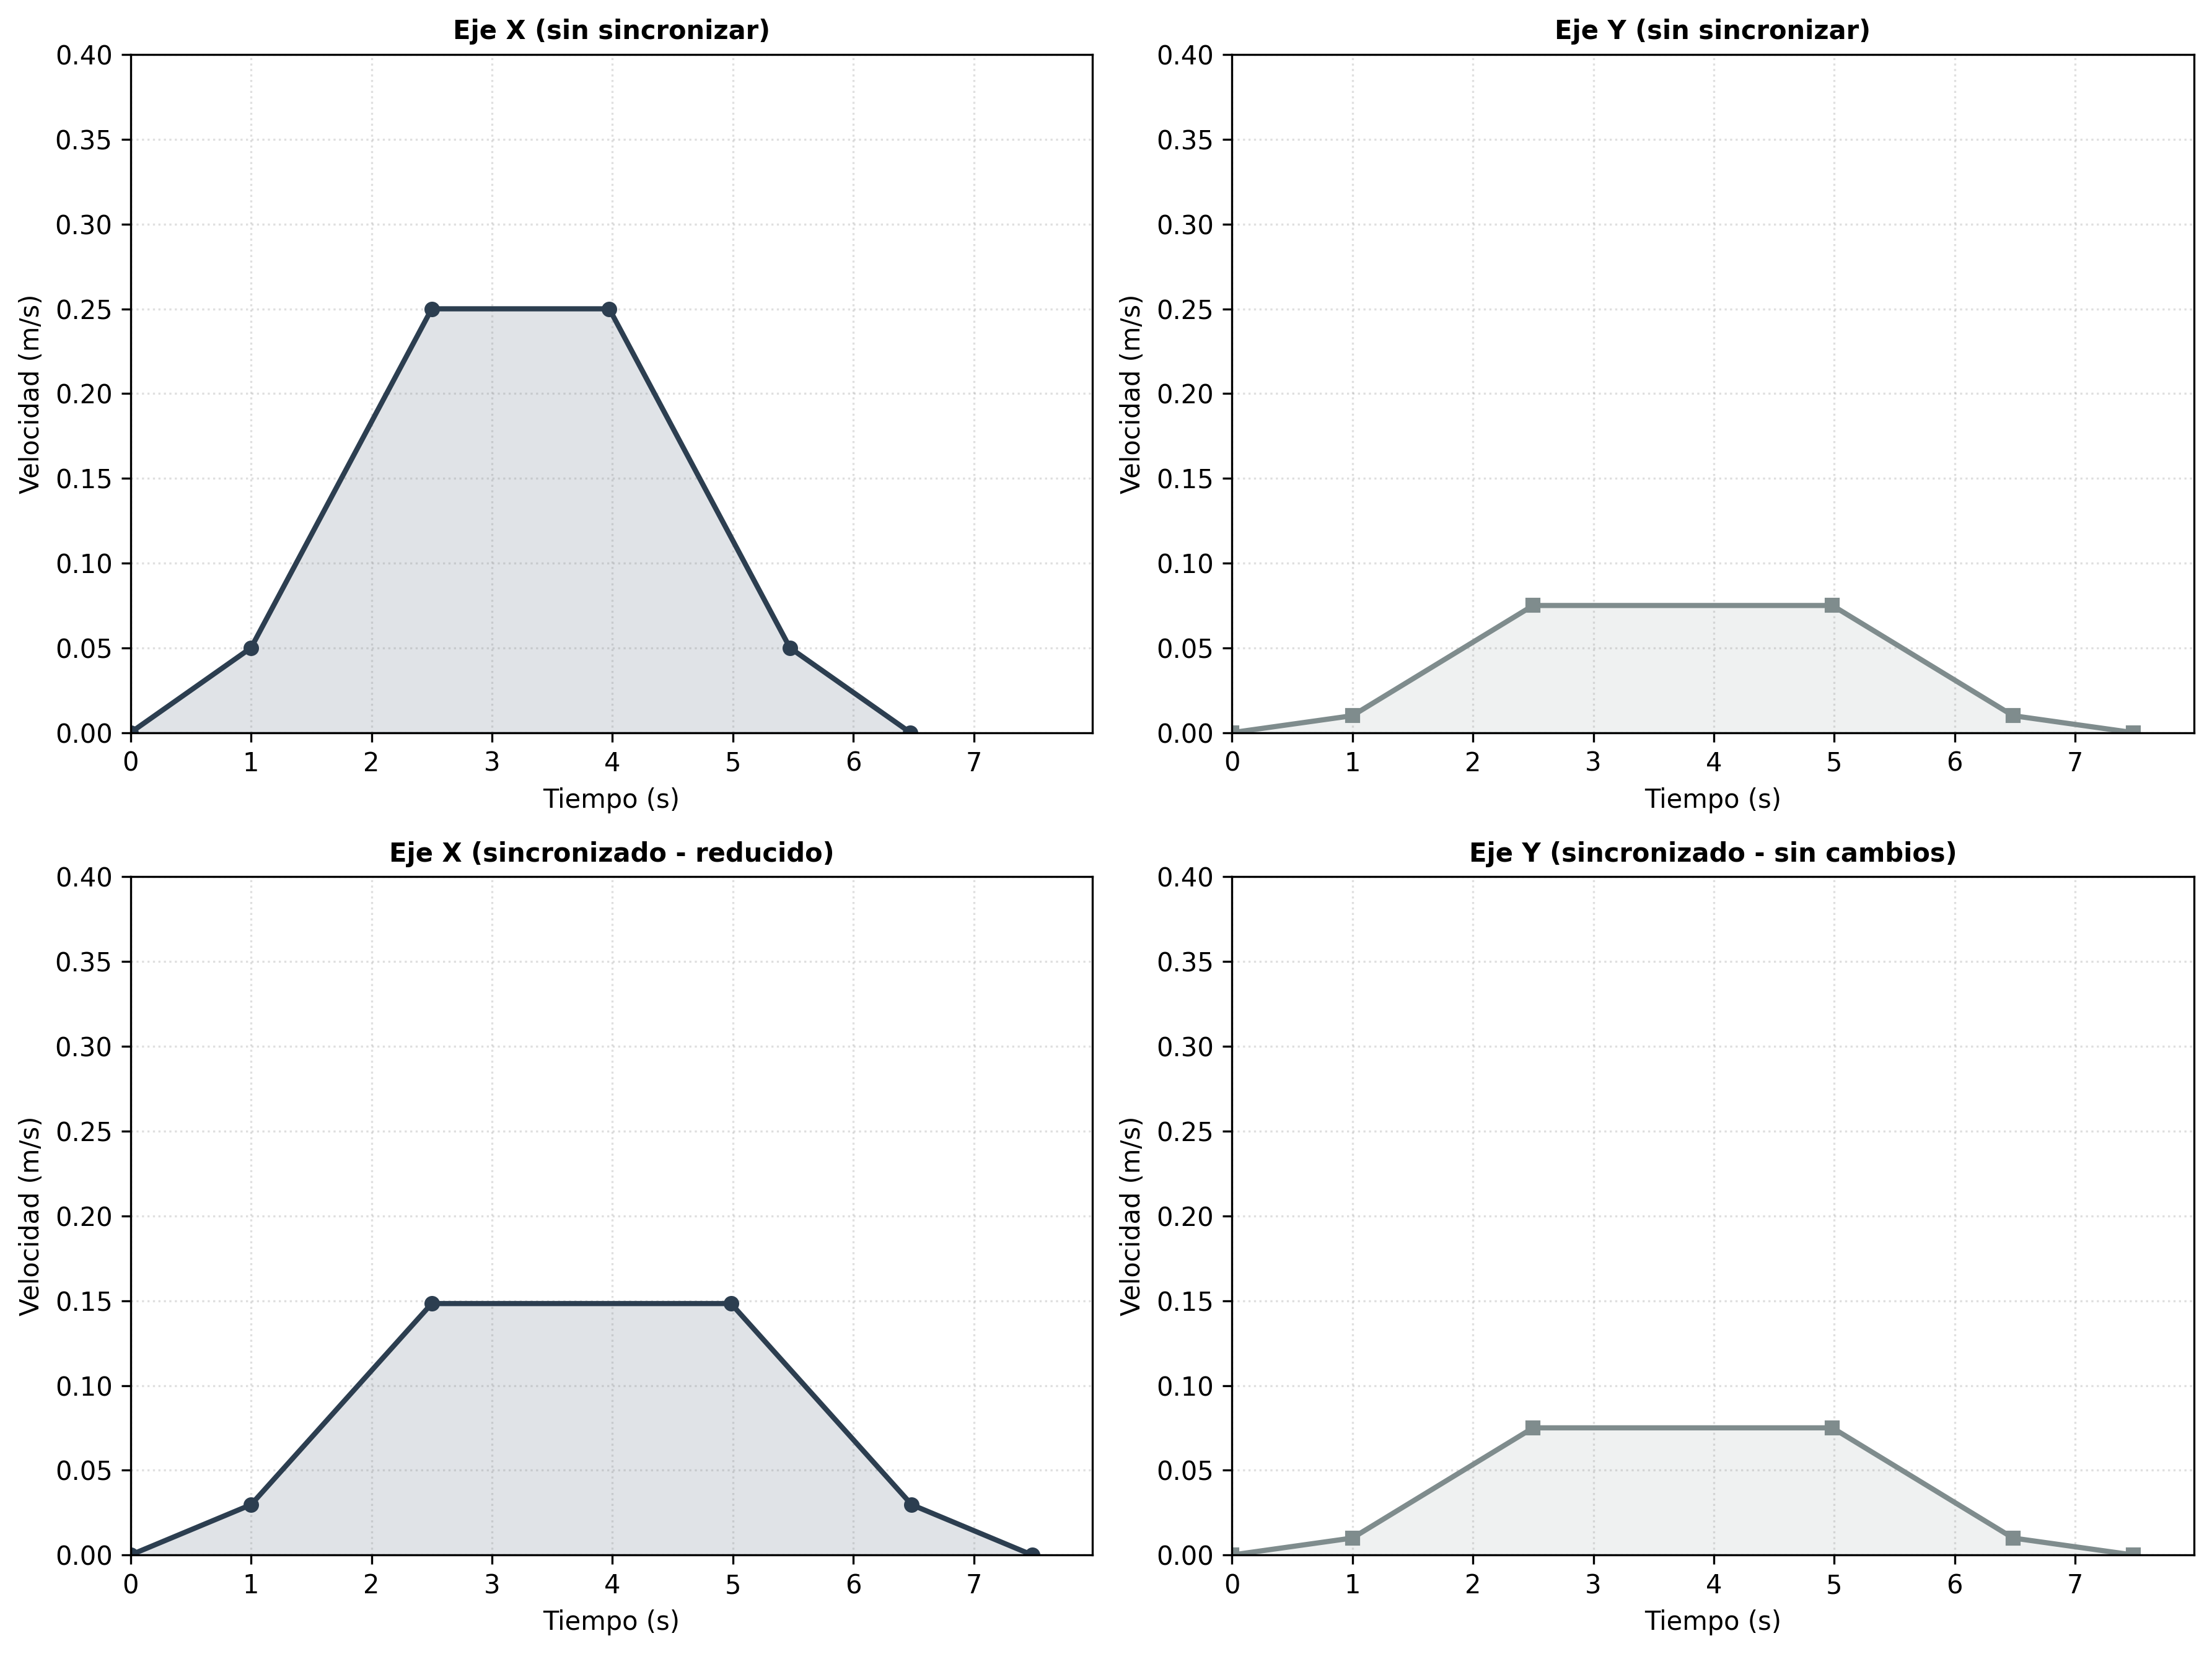
\includegraphics[width=0.7\textwidth]{imagenes/sincronizacion_multieje.png}
    \caption{Sincronización de perfiles de velocidad para movimientos diagonales mediante escalamiento proporcional}
    \label{fig:sincronizacion_multieje}
\end{figure}

El Timer1 genera interrupciones a frecuencia configurable que alternan el estado del pin STEP entre alto y bajo, creando los pulsos necesarios para el driver TB6600. Cada transición alto-bajo constituye un paso del motor. El sistema cuenta los pasos ejecutados y controla la frecuencia de interrupción mediante el registro de comparación OCR1A del timer:

\begin{equation}
f_{step} = \frac{f_{CPU}}{2 \cdot prescaler \cdot (OCR1A + 1)}
\end{equation}

donde $f_{CPU} = 16$ MHz, prescaler = 8, y OCR1A se calcula dinámicamente.

Para una velocidad deseada $v$ en pasos/s, el valor de OCR1A es:

\begin{equation}
OCR1A = \frac{f_{CPU}}{2 \cdot prescaler \cdot v} - 1 = \frac{16000000}{2 \cdot 8 \cdot v} - 1 = \frac{1000000}{v} - 1
\end{equation}

El firmware precalcula y limita OCR1A para evitar overflow y garantizar estabilidad.
La conversión entre pasos de motor y desplazamiento lineal depende de las características mecánicas de cada eje. Los motores NEMA 17 utilizados tienen 200 pasos por revolución, configurados con microstepping 1/8 en los drivers TB6600, resultando en 1600 pasos por revolución efectiva.

\textbf{Eje Horizontal:} Utiliza transmisión por correa dentada GT2 con polea de 20 dientes y paso de 2mm, generando 40mm de avance lineal por revolución del motor. La conversión resulta:
\begin{equation}
\text{Pasos/mm}_H = \frac{1600 \text{ pasos/rev}}{40 \text{ mm/rev}} = 40 \text{ pasos/mm}
\end{equation}

\textbf{Eje Vertical:} Utiliza transmisión por varilla roscada M8 con paso de rosca de 1.25mm, generando 8mm de avance lineal por revolución del motor (rosca de 4 entradas). La conversión resulta:
\begin{equation}
\text{Pasos/mm}_V = \frac{1600 \text{ pasos/rev}}{8 \text{ mm/rev}} = 200 \text{ pasos/mm}
\end{equation}

Estos valores se definen como constantes en el archivo de configuración (system\_config.h) mediante las macros STEPS\_PER\_MM\_H y STEPS\_PER\_MM\_V. El firmware utiliza estas conversiones para traducir comandos en milímetros a cantidad de pasos que debe ejecutar cada motor.

\begin{table}[H]
\centering
\begin{tabular}{|l|c|c|c|c|}
\hline
\textbf{Eje} & \textbf{Transmisión} & \textbf{mm/rev} & \textbf{Pasos/rev} & \textbf{Pasos/mm} \\
\hline
Horizontal & Correa GT2 & 40 & 1600 & 40 \\
\hline
Vertical & Varilla M8 & 8 & 1600 & 200 \\
\hline
\end{tabular}
\caption{Conversiones mecánicas de los ejes de movimiento}
\label{tab:conversiones_mecanicas}
\end{table}


\subsection{Protocolo de comunicación UART}
% Estructura Comandos


\subsubsection{Manejo de errores y protecciones}

El firmware implementa mecanismos robustos de detección y manejo de errores para garantizar operación segura del sistema mecánico.

Antes de ejecutar cualquier comando, el analizador sintáctico valida sintaxis y rangos. Comandos inválidos retornan código de error inmediatamente sin ejecutar acción, previniendo movimientos peligrosos (Tabla \ref{tab:validacion_comandos}).

\begin{table}[H]
\centering
\small
\begin{tabular}{|l|l|l|}
\hline
Parámetro & Rango válido & Error \\
\hline
Delimitadores & \texttt{<} y \texttt{>} presentes & INVALID\_CMD \\
\hline
Velocidad H & 500 - 15,000 pasos/s & INVALID\_PARAM \\
\hline
Velocidad V & 500 - 12,000 pasos/s & INVALID\_PARAM \\
\hline
Ángulo servo & 10° - 160° & INVALID\_PARAM \\
\hline
Tiempo trayectoria & 0 - 10,000 ms & INVALID\_PARAM \\
\hline
\end{tabular}
\caption{\textit{Validaciones de comandos y rangos permitidos}}
\label{tab:validacion_comandos}
\end{table}

El firmware implementa supervisor de comunicación: si no recibe señal de sincronización (\texttt{HB:1}) del nivel superior durante un período prolongado, asume pérdida de comunicación y ejecuta detención de emergencia automática, deshabilitando todos los motores y entrando en modo seguro hasta recibir comando de reset.

El buffer UART circular (256 bytes) implementa protección contra overflow verificando espacio disponible antes de cada escritura. Si el buffer está lleno, el byte se descarta y se envía error de overflow. La Tabla \ref{tab:codigos_error} lista los códigos de error definidos.

\begin{table}[H]
\centering
\begin{tabular}{|l|p{9cm}|}
\hline
Código & Descripción y causa \\
\hline
INVALID\_CMD & Comando no reconocido o sintaxis incorrecta. \\
\hline
INVALID\_PARAM & Parámetros fuera de rango válido. \\
\hline
LIMIT\_HIT & Movimiento bloqueado por activación de final de carrera. \\
\hline
BUFFER\_OVERFLOW & Buffer UART saturado. \\
\hline
TIMEOUT & Operación excedió tiempo límite configurado. \\
\hline
SYSTEM\_ERROR & Error interno del firmware. \\
\hline
\end{tabular}
\caption{\textit{Códigos de error del firmware}}
\label{tab:codigos_error}
\end{table}

Los finales de carrera se monitorean continuamente. El sistema detecta la activación de cualquier límite y ejecuta inmediatamente la detención de emergencia: deshabilita los drivers (ENABLE = HIGH), detiene la generación de pulsos, envía notificación asíncrona al supervisor indicando el límite activado, y bloquea nuevos comandos de movimiento hacia el lado en el que se encuentra el fin de carrera. Esto previene daños mecánicos por intentos de movimiento en dirección bloqueada.


\section{Nivel supervisor}

\subsection{Arquitectura del software}
El software del nivel supervisor se implementa en Python 3 siguiendo una arquitectura modular que separa responsabilidades en capas funcionales específicas. La Figura \ref{fig:arquitectura_modulos_supervisor} muestra la organización de módulos y sus dependencias.

\textbf{Capa de Hardware}: Gestiona la comunicación con el nivel regulatorio y la adquisición de imágenes. El módulo UARTManager implementa comunicación serial mediante puerto USB a 115200 baudios, utilizando callbacks para procesamiento asíncrono de mensajes recibidos del firmware. El módulo CommandManager proporciona métodos de alto nivel para enviar comandos estructurados al nivel regulatorio.

\textbf{Capa de Control}: Coordina el estado global del robot. El módulo RobotController mantiene el seguimiento de posición global mediante acumulación de desplazamientos reportados por el firmware, detecta y maneja eventos mediante callbacks, y gestiona la persistencia de estado en archivos JSON. El módulo CameraManager centraliza el acceso a la cámara USB evitando conflictos de acceso concurrente.

\textbf{Capa de Robot}: Implementa el control del brazo robótico. El módulo ArmController define cuatro posiciones operacionales discretas con ángulos específicos de servomotores y genera trayectorias mediante interpolación lineal.

\textbf{Capa de Procesos}: Define las secuencias de alto nivel del robot. El módulo workflow\_orchestrator implementa los cuatro procesos principales del sistema: homing, calibración del workspace, mapeo del entorno, y cosecha interactiva.

\begin{figure}[H]
    \centering
    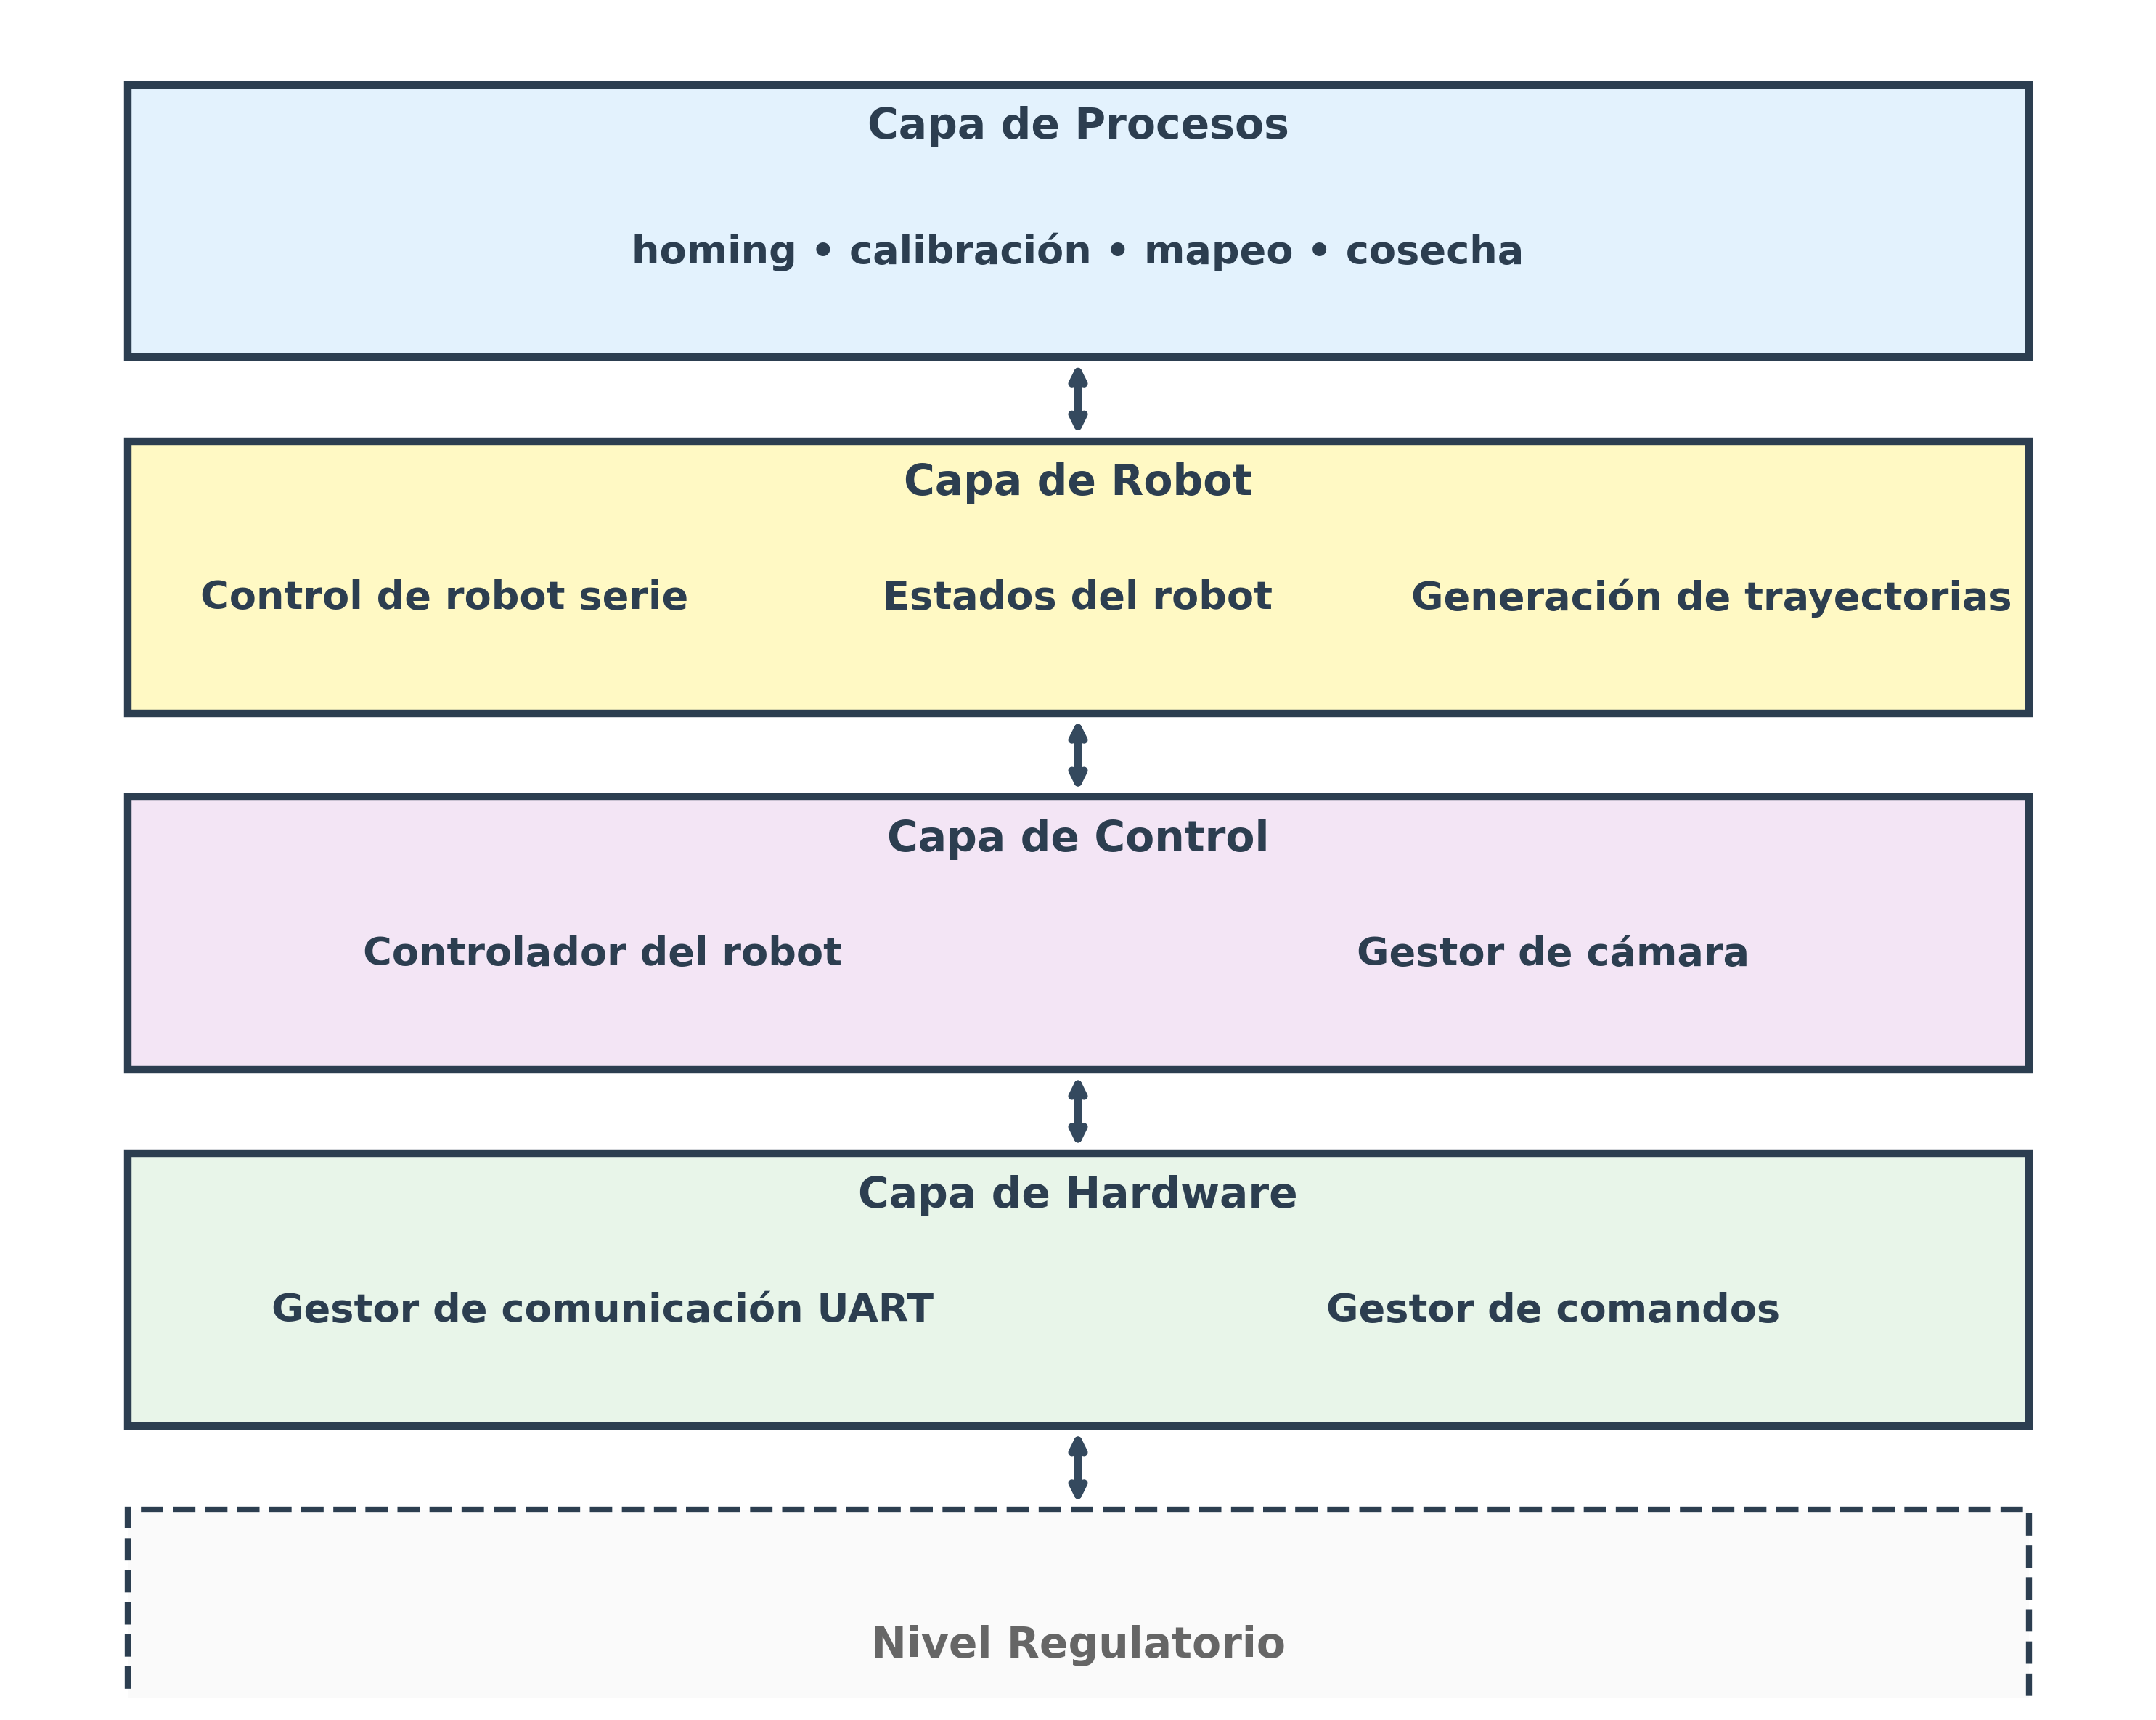
\includegraphics[width=0.8\textwidth]{imagenes/arquitectura_modulos_supervisor.png}
    \caption{\textit{Arquitectura modular del software supervisor mostrando capas y flujo de información}}
    \label{fig:arquitectura_modulos_supervisor}
\end{figure}

\subsection{Funcionalidad y procesos}
El nivel supervisor constituye la capa de coordinación del sistema, responsable de orquestar tareas complejas que requieren la integración de múltiples subsistemas. A diferencia del nivel regulatorio que ejecuta comandos individuales (mover X milímetros, activar gripper), el supervisor planifica secuencias completas de acciones para lograr objetivos de alto nivel como mapear el entorno o cosechar plantas.

\textbf{Responsabilidades principales:}

\begin{itemize}
    \item \textbf{Planificación de secuencias}: Descompone tareas complejas (ej: "cosechar lechuga en posición X,Y") en secuencias ordenadas de comandos básicos. Determina qué hacer primero, qué condiciones verificar, y cómo responder ante eventos inesperados.

    \item \textbf{Gestión de estado global}: Mantiene información sobre el sistema que el nivel regulatorio no conoce: posición global acumulada desde el homing, dimensiones calibradas del workspace, mapas de ubicaciones de tubos y plantas, y estado del proceso en ejecución. Este estado se actualiza mediante callbacks que procesan mensajes asíncronos del firmware (STEPPER\_MOVE\_COMPLETED, LIMIT\_TRIGGERED).

    \item \textbf{Integración con visión}: Invoca algoritmos de procesamiento de imágenes en momentos específicos de las secuencias, interpreta sus resultados (coordenadas, clasificaciones), y ajusta el plan según lo detectado. Por ejemplo, durante el mapeo decide cuándo capturar imágenes para buscar tubos, y durante la cosecha decide si recolectar una planta según su clasificación morfológica.

    \item \textbf{Comunicación bidireccional}: Envía comandos al nivel regulatorio mediante mensajes UART (formato \texttt{<COMANDO:params>}) y espera respuestas que confirman ejecución exitosa o reportan errores. Actualiza su estado interno según las notificaciones recibidas. Envía señales de sincronización periódicas para que el firmware detecte si el supervisor falló.

    \item \textbf{Persistencia de información}: Guarda datos críticos en archivos JSON que sobreviven reinicios del sistema: referencia de origen tras homing (homing\_reference.json), dimensiones medidas del workspace (workspace\_dimensions.json), última posición conocida (current\_position.json), posiciones Y de tubos detectados (configuracion\_tubos.json), y posiciones X de plantas (matriz\_cintas.json).
\end{itemize}

\textbf{Modelo de ejecución orientado a eventos:}

El supervisor no utiliza hilos concurrentes sino un modelo orientado a eventos mediante callbacks. Cuando envía un comando de movimiento al firmware, no espera bloqueado a que termine. En cambio, registra un callback que será invocado cuando llegue el mensaje \texttt{STEPPER\_MOVE\_COMPLETED}. Durante la espera, el bucle principal del programa continúa procesando otros eventos (mensajes UART entrantes, capturas de cámara). Este diseño evita bloqueos y permite respuesta inmediata a eventos inesperados como activación de finales de carrera.

\subsubsection{Procesos Implementados}

El sistema implementa cuatro procesos principales que coordinan movimientos, captura de imágenes, y ejecución de algoritmos de visión. Cada proceso verifica precondiciones antes de ejecutar acciones críticas (sistema referenciado, brazo en posición compatible, cámara disponible).

\textbf{Proceso 1: Homing (Referenciado del Sistema)}

Establece el origen del sistema de coordenadas moviendo los ejes hasta los finales de carrera y retrocediendo offsets calibrados.

\begin{table}[H]
\centering
\small
\begin{tabular}{|l|p{10cm}|}
\hline
\textbf{Paso} & \textbf{Acción} \\
\hline
1. Verificación inicial & Confirma que el brazo está en posición de movimiento (servos retraídos). Si no lo está, ejecuta transición de brazo antes de continuar. \\
\hline
2. Configuración & Reduce velocidades a HOMING\_SPEED\_H y HOMING\_SPEED\_V (más lentas que velocidades normales para evitar impactos bruscos contra límites). \\
\hline
3. Homing horizontal & Envía comando de movimiento hacia la derecha con distancia muy grande (500mm, mayor que el workspace). El firmware detiene el movimiento al activarse el final de carrera H\_RIGHT. Envía comando de retroceso de HOME\_OFFSET\_H milímetros. \\
\hline
4. Homing vertical & Envía comando de movimiento hacia arriba con distancia muy grande. El firmware detiene al activarse V\_UP. Retrocede HOME\_OFFSET\_V milímetros. \\
\hline
5. Establecer origen & Envía comando \texttt{<XY:0,0>} al firmware para que establezca la posición actual como (0,0). Actualiza el estado global del supervisor a (0,0). \\
\hline
6. Restauración & Restaura velocidades normales (NORMAL\_SPEED\_H, NORMAL\_SPEED\_V). \\
\hline
7. Persistencia & Guarda la referencia en homing\_reference.json con timestamp para verificaciones futuras. \\
\hline
\end{tabular}
\caption{Secuencia del proceso de homing}
\label{tab:proceso_homing}
\end{table}

\textbf{Proceso 2: Calibración del espacio de trabajo}

Mide las dimensiones útiles del espacio de trabajo moviendo los ejes hasta sus límites opuestos.

\begin{table}[H]
\centering
\small
\begin{tabular}{|l|p{10cm}|}
\hline
\textbf{Paso} & \textbf{Acción} \\
\hline
1. Homing inicial & Ejecuta proceso de homing para partir desde origen conocido. \\
\hline
2. Medición horizontal & Intenta mover hacia la izquierda una distancia muy grande. El firmware detiene al activar H\_LEFT y envía mensaje de emergencia. El supervisor registra la distancia recorrida como ancho bruto del workspace. \\
\hline
3. Retorno horizontal & Mueve hacia la derecha la distancia registrada más un margen para volver cerca del origen horizontal. \\
\hline
4. Medición vertical & Intenta mover hacia abajo una distancia muy grande. El firmware detiene al activar V\_DOWN. Registra la distancia como alto bruto. \\
\hline
5. Cálculo de dimensiones & Resta márgenes de seguridad (5-10mm) del ancho y alto brutos para obtener dimensiones útiles MAX\_X y MAX\_Y. \\
\hline
6. Homing final & Ejecuta homing nuevamente para volver al origen. \\
\hline
7. Persistencia & Guarda MAX\_X y MAX\_Y en workspace\_dimensions.json. \\
\hline
\end{tabular}
\caption{Secuencia del proceso de calibración}
\label{tab:proceso_calibracion}
\end{table}

\textbf{Proceso 3: Mapeo del Entorno}

Escanea el workspace para detectar posiciones de tubos (coordenadas Y) y plantas (coordenadas X), generando mapas que guían la navegación posterior.

\begin{table}[H]
\centering
\small
\begin{tabular}{|l|p{10cm}|}
\hline
\textbf{Paso} & \textbf{Acción} \\
\hline
1. Escaneo vertical & Desde el origen, mueve el eje vertical hacia abajo en pasos incrementales (ej: cada 5mm). En cada pausa, captura imagen y ejecuta detector de tubos. Si detecta tubo, registra coordenada Y en lista temporal. Continúa hasta recorrer todo el alto del workspace. \\
\hline
2. Guardado de tubos & Ordena las coordenadas Y detectadas de mayor a menor. Las guarda en configuracion\_tubos.json con formato: \texttt{\{"1": \{"y\_mm": 250, "nombre": "Tubo 1"\}, "2": \{...\}\}}. \\
\hline
3. Escaneos horizontales & Para cada tubo en configuracion\_tubos.json: mueve el sistema a la coordenada Y del tubo, ejecuta barrido horizontal desde X=0 hacia la derecha en pasos incrementales, en cada pausa captura imagen y ejecuta detector de cintas, si detecta cinta negra registra coordenada X en lista temporal del tubo. \\
\hline
4. Guardado de cintas & Para cada tubo, guarda las coordenadas X detectadas en matriz\_cintas.json con formato: \texttt{\{"tubo\_1": [50, 120, 190, ...], "tubo\_2": [...]\}}. \\
\hline
5. Retorno & Mueve el sistema de vuelta al origen (0,0). \\
\hline
\end{tabular}
\caption{Secuencia del proceso de mapeo}
\label{tab:proceso_mapeo}
\end{table}

\textbf{Proceso 4: Cosecha Interactiva}

Navega a cada posición registrada en matriz\_cintas.json, clasifica la planta, y si está madura ejecuta la recolección.

\begin{table}[H]
\centering
\small
\begin{tabular}{|l|p{10cm}|}
\hline
\textbf{Paso} & \textbf{Acción} \\
\hline
1. Carga de mapas & Lee configuracion\_tubos.json y matriz\_cintas.json. Valida que existan datos. Genera lista de posiciones (X,Y) a visitar iterando tubos y sus cintas. \\
\hline
2. Navegación & Para cada posición (X,Y): mueve el sistema XY a esa coordenada, espera confirmación de llegada del firmware. \\
\hline
3. Clasificación & Captura imagen con la cámara. Ejecuta clasificador morfológico que retorna: clase predicha (LECHUGA, PLANTIN, VASO\_VACIO, etc.) y confianza (0-1). \\
\hline
4. Decisión & Si clase es LECHUGA: ejecuta corrección de posición con detectores de cintas para centrar la planta bajo el gripper (ajustes de ±10mm típicamente), transfiere el brazo de posición "movimiento" a "recoger" (servos se extienden hacia planta), envía comando de cierre del gripper, espera confirmación GRIPPER\_CLOSED, transfiere brazo a posición "transportar" (eleva planta). \\
\hline
5. Depósito & Si tiene planta en gripper: navega a zona de depósito (coordenadas predefinidas cerca de un borde), transfiere brazo a posición "depositar" (inclina hacia contenedor), abre gripper, espera confirmación GRIPPER\_OPENED, transfiere brazo a "transportar". \\
\hline
6. Continuación & Si quedan posiciones por procesar, vuelve al paso 2. Si no, procede al paso 7. \\
\hline
7. Finalización & Navega de vuelta al origen (0,0). Transfiere brazo a posición "movimiento". Registra estadísticas: plantas cosechadas, vasos vacíos, plantas inmaduras. \\
\hline
\end{tabular}
\caption{Secuencia del proceso de cosecha interactiva}
\label{tab:proceso_cosecha}
\end{table}

\textbf{Manejo de errores durante procesos:}

Durante la ejecución de cualquier proceso, el supervisor monitorea eventos inesperados:

\begin{itemize}
    \item \textbf{Límite activado inesperadamente}: Si recibe LIMIT\_TRIGGERED durante un movimiento que no debería alcanzar límites, detiene el proceso, registra el error, y preserva el estado para diagnóstico.
    \item \textbf{Pérdida de comunicación}: Si un comando no recibe respuesta en tiempo límite configurado (ej: 30s para movimientos largos), aborta el proceso e intenta re-establecer comunicación.
    \item \textbf{Fallo de detector}: Si un algoritmo de visión no retorna resultados válidos (ej: no detecta tubo esperado), registra la falla e intenta continuar con la siguiente posición, o solicita intervención del usuario según la severidad.
\end{itemize}

\begin{figure}[H]
    \centering
    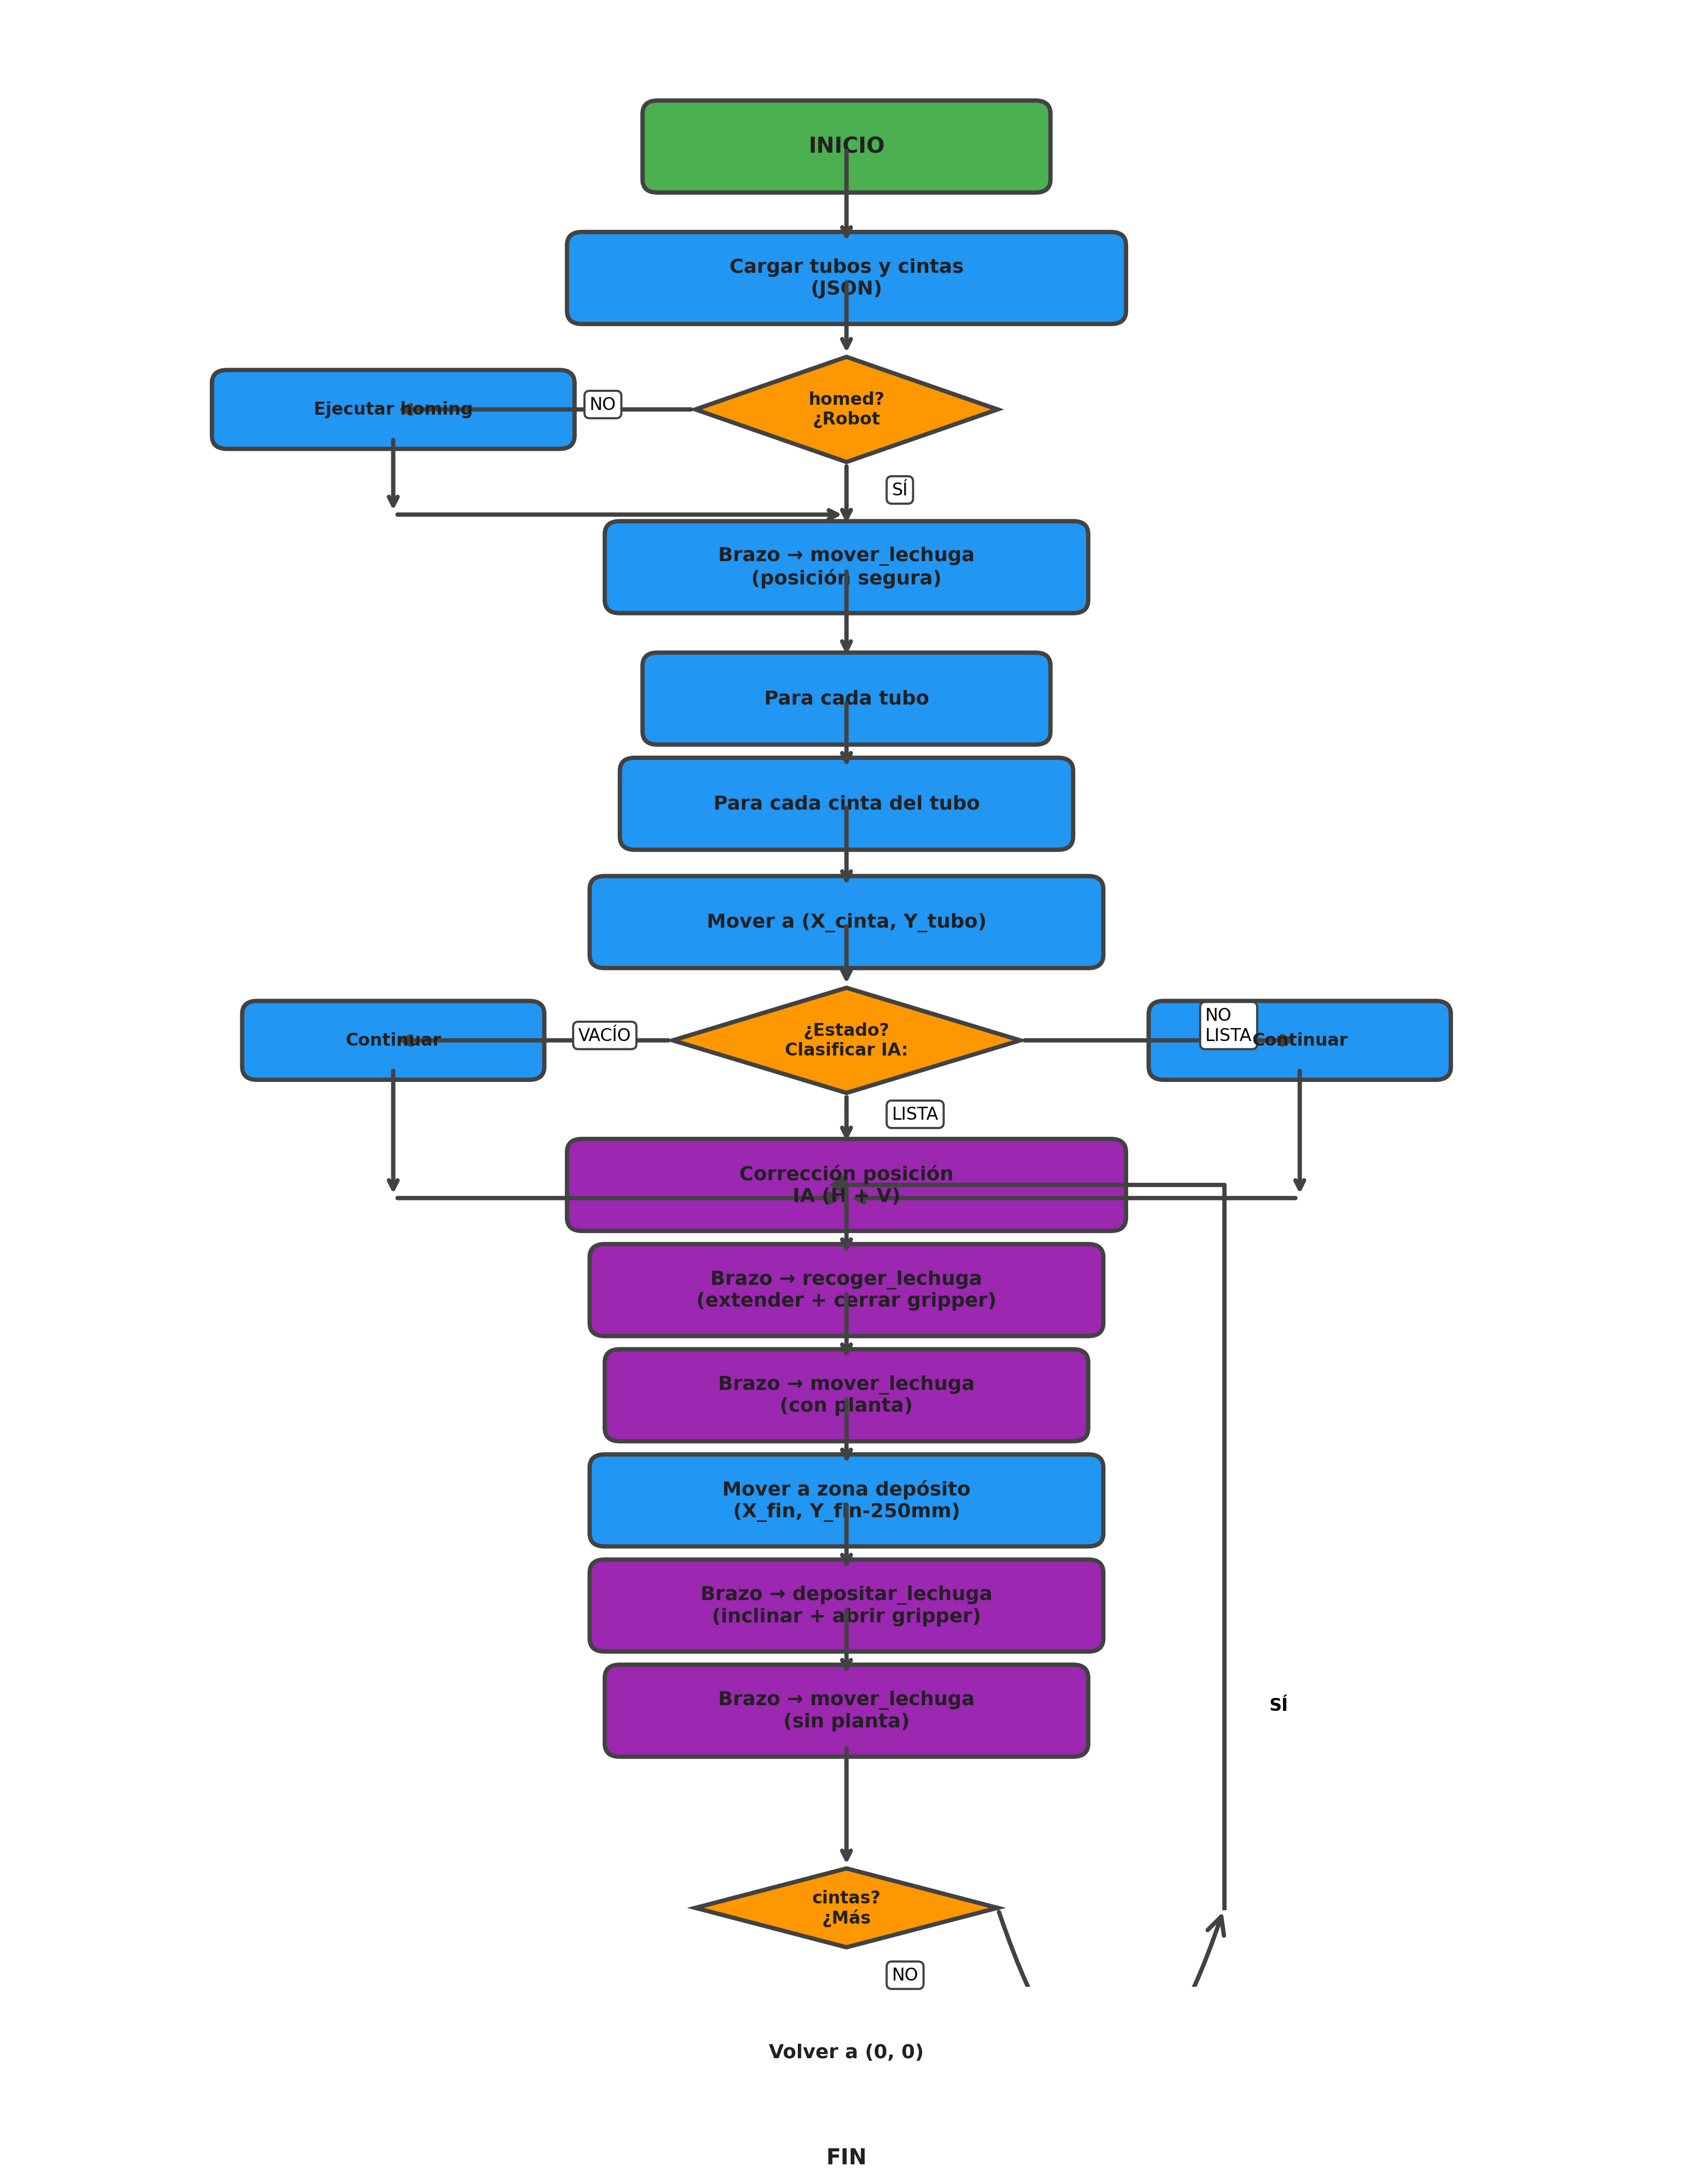
\includegraphics[width=0.85\textwidth]{imagenes/diagrama_flujo_cosecha.png}
    \caption{Diagrama de flujo detallado del proceso de cosecha mostrando decisiones según clasificación}
    \label{fig:flujo_cosecha}
\end{figure}


\subsection{Seguimiento de posición global}
\subsubsection{Seguimiento de Posición Global}

El sistema supervisor mantiene un seguimiento continuo de la posición del robot mediante movimientos relativos y confirmaciones del nivel regulatorio.

El supervisor envía comandos especificando desplazamientos incrementales respecto a la posición actual. Al completar cada movimiento, el nivel regulatorio notifica el desplazamiento real ejecutado, que puede diferir del solicitado si se activa un límite físico durante la trayectoria. Un proceso de monitoreo continuo detecta estas confirmaciones y actualiza la posición global mediante suma acumulativa de los desplazamientos reportados.

Durante el proceso de homing, los eventos de activación de finales de carrera se utilizan para establecer el origen del sistema de coordenadas. En operación normal, si un límite se activa inesperadamente, el firmware detiene el movimiento y notifica tanto el desplazamiento parcial ejecutado como la activación del límite correspondiente.
El supervisor ajusta la posición global en consecuencia, asegurando que la representación interna del estado del robot refleje con precisión su ubicación física. Este enfoque permite una gestión robusta de la posición, incluso en presencia de errores o interrupciones inesperadas durante el movimiento.


\subsection{Control del brazo robótico}
El control del brazo se implementa mediante una máquina de estados finitos que define cuatro posiciones operacionales discretas. Cada posición corresponde a una configuración angular específica de los servomotores, optimizada para una fase del ciclo de cosecha (Tabla \ref{tab:estados_brazo}).

\begin{table}[H]
\centering
\small
\begin{tabular}{|l|c|c|c|p{4.5cm}|}
\hline
\textbf{Posición} & \textbf{Servo 1} & \textbf{Servo 2} & \textbf{Gripper} & \textbf{Función} \\
\hline
Movimiento & 10° & 10° & Cualquiera & Brazo plegado para desplazamientos XY \\
\hline
Recoger & 100° & 80° & Abierto & Aproximación para recolección \\
\hline
Transportar & 50° & 160° & Cerrado & Transporte seguro de planta \\
\hline
Depositar & 90° & 20° & Abierto & Liberación sobre contenedor \\
\hline
\end{tabular}
\caption{Posiciones operacionales del brazo robótico}
\label{tab:estados_brazo}
\end{table}

\begin{figure}[H]
    \centering
    % Fila superior
    \begin{subfigure}[b]{0.35\textwidth}
        \centering
        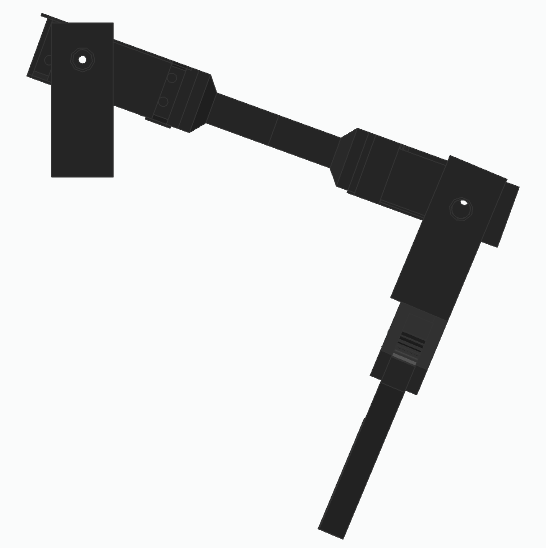
\includegraphics[width=\textwidth]{imagenes/brazo_movimiento.png}
        \caption{Posición Movimiento}
    \end{subfigure}
    \hfill
    \begin{subfigure}[b]{0.35\textwidth}
        \centering
        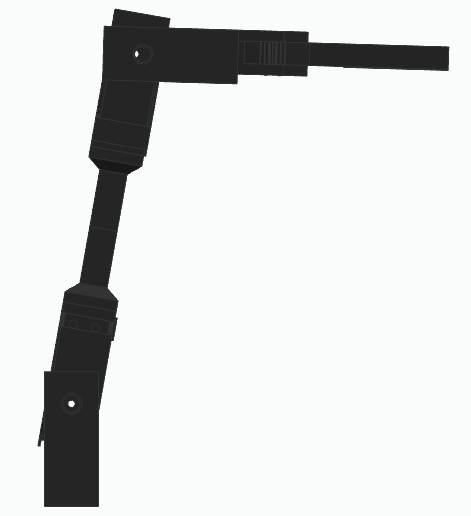
\includegraphics[width=\textwidth]{imagenes/brazo_transportar.png}
        \caption{Posición Transportar}
    \end{subfigure}

    % Espacio moderado entre filas
    \vspace{0.25cm}

    % Fila inferior
    \begin{subfigure}[b]{0.45\textwidth}
        \centering
        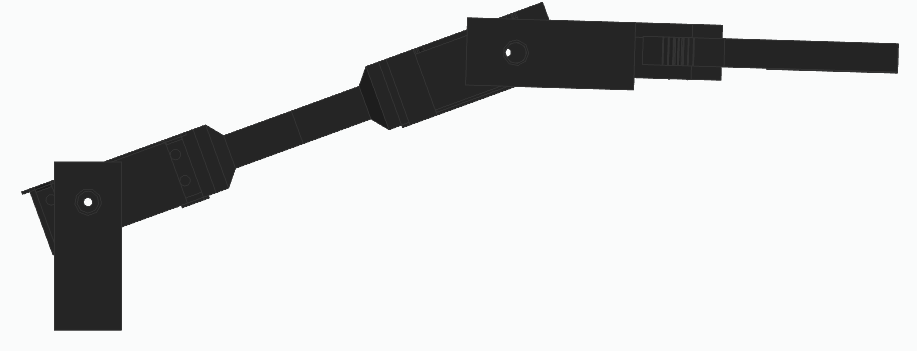
\includegraphics[width=\textwidth]{imagenes/brazo_recoger.png}
        \caption{Posición Recoger}
    \end{subfigure}
    \hfill
    \begin{subfigure}[b]{0.45\textwidth}
        \centering
        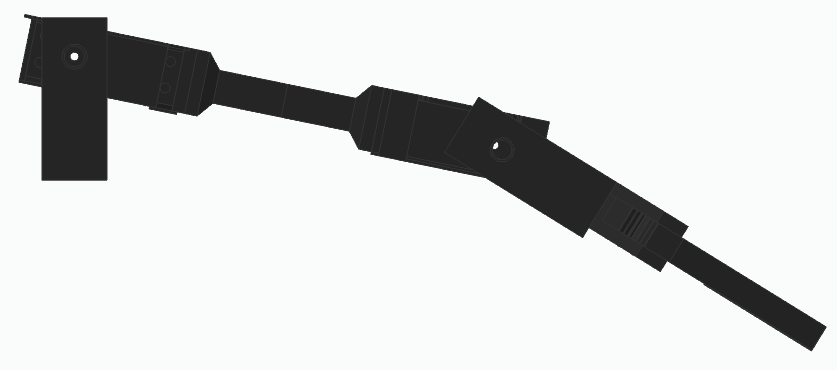
\includegraphics[width=\textwidth]{imagenes/brazo_depositar.png}
        \caption{Posición Depositar}
    \end{subfigure}

    \caption{Cuatro posiciones operacionales del brazo robótico}
    \label{fig:posiciones_brazo}
\end{figure}


Las transiciones entre posiciones se ejecutan mediante interpolación lineal de ángulos. Dada una transición desde la posición A hacia la posición B, el sistema genera una trayectoria continua dividida en puntos intermedios muestreados cada 50ms durante un período $T$ de 1 a 3 segundos. Para cada servomotor $i$, el ángulo en el instante $t$ se calcula según:

\begin{equation}
\theta_i(t) = \theta_i^A + \frac{t}{T} \cdot (\theta_i^B - \theta_i^A)
\end{equation}

Esta interpolación garantiza movimientos suaves que minimizan vibraciones mecánicas y cargas sobre los actuadores. Las transiciones están reguladas por condiciones que verifican la validez de cada cambio de estado, evitando secuencias que comprometan la seguridad o integridad del sistema. 

Los movimientos del sistema cartesiano solo se permiten cuando el brazo se encuentra en posición de movimiento o transporte, garantizando que no ocurran colisiones durante desplazamientos. Mientras el brazo ejecuta una trayectoria de transición, se bloquean tanto comandos de movimiento XY como nuevas transiciones del brazo. Para algunos movimientos críticos, el robot debe estar en una posición XY determinada para evitar colisiones con el entorno.

\subsection{Manejo de errores y recuperación}
\subsubsection{Manejo de errores y protecciones}

El firmware implementa mecanismos robustos de detección y manejo de errores para garantizar operación segura del sistema mecánico.

Antes de ejecutar cualquier comando, el analizador sintáctico valida sintaxis y rangos. Comandos inválidos retornan código de error inmediatamente sin ejecutar acción, previniendo movimientos peligrosos (Tabla \ref{tab:validacion_comandos}).

\begin{table}[H]
\centering
\small
\begin{tabular}{|l|l|l|}
\hline
Parámetro & Rango válido & Error \\
\hline
Delimitadores & \texttt{<} y \texttt{>} presentes & INVALID\_CMD \\
\hline
Velocidad H & 500 - 15,000 pasos/s & INVALID\_PARAM \\
\hline
Velocidad V & 500 - 12,000 pasos/s & INVALID\_PARAM \\
\hline
Ángulo servo & 10° - 160° & INVALID\_PARAM \\
\hline
Tiempo trayectoria & 0 - 10,000 ms & INVALID\_PARAM \\
\hline
\end{tabular}
\caption{\textit{Validaciones de comandos y rangos permitidos}}
\label{tab:validacion_comandos}
\end{table}

El firmware implementa supervisor de comunicación: si no recibe señal de sincronización (\texttt{HB:1}) del nivel superior durante un período prolongado, asume pérdida de comunicación y ejecuta detención de emergencia automática, deshabilitando todos los motores y entrando en modo seguro hasta recibir comando de reset.

El buffer UART circular (256 bytes) implementa protección contra overflow verificando espacio disponible antes de cada escritura. Si el buffer está lleno, el byte se descarta y se envía error de overflow. La Tabla \ref{tab:codigos_error} lista los códigos de error definidos.

\begin{table}[H]
\centering
\begin{tabular}{|l|p{9cm}|}
\hline
Código & Descripción y causa \\
\hline
INVALID\_CMD & Comando no reconocido o sintaxis incorrecta. \\
\hline
INVALID\_PARAM & Parámetros fuera de rango válido. \\
\hline
LIMIT\_HIT & Movimiento bloqueado por activación de final de carrera. \\
\hline
BUFFER\_OVERFLOW & Buffer UART saturado. \\
\hline
TIMEOUT & Operación excedió tiempo límite configurado. \\
\hline
SYSTEM\_ERROR & Error interno del firmware. \\
\hline
\end{tabular}
\caption{\textit{Códigos de error del firmware}}
\label{tab:codigos_error}
\end{table}

Los finales de carrera se monitorean continuamente. El sistema detecta la activación de cualquier límite y ejecuta inmediatamente la detención de emergencia: deshabilita los drivers (ENABLE = HIGH), detiene la generación de pulsos, envía notificación asíncrona al supervisor indicando el límite activado, y bloquea nuevos comandos de movimiento hacia el lado en el que se encuentra el fin de carrera. Esto previene daños mecánicos por intentos de movimiento en dirección bloqueada.


\section{Inteligencia artificial y visión por computadora}

\subsection{Arquitectura y procesamiento}
El sistema de visión por computadora se estructura en tres módulos especializados que operan de manera coordinada durante los procesos de exploración y cosecha:\\

\underline{Detector de tubos de cultivo:} Identifica tubos de PVC mediante análisis de bordes y saturación durante el escaneo vertical del workspace. Utiliza el algoritmo de Canny combinado con filtrado en el canal de saturación (HSV) para detectar los bordes superior e inferior de cada tubo. Registra las posiciones verticales \textbf{Y} de todos los tubos detectados, generando un archivo configuracion\_tubos.json que permite al sistema ubicar cada fila de cultivo.\\

\underline{Detector de cintas de referencia:} Localiza cintas negras adhesivas de 18mm de ancho mediante umbralización inversa del canal V (HSV). Opera en tres contextos: corrección de posición horizontal (centroide de cinta vertical), corrección de posición vertical (arista base de cinta), y escaneo horizontal para registrar posiciones \textbf{X} de plantas en matriz\_cintas.json.\\

\underline{Clasificador morfológico de cultivos:} Determina el estado de madurez mediante análisis del área de vegetación verde segmentada. Aplica umbralización en el espacio HSV para extraer píxeles verdes, refinamiento morfológico (cierre y apertura), detección de contornos, y clasificación por umbral de área estadísticamente determinado. Discrimina entre lechugas maduras (área mayor al umbral), plantas inmaduras, y posiciones vacías.


\subsection{Detector de marcadores de referencia}
\subsubsection{Fundamento}

El detector de marcadores implementa un algoritmo basado en segmentación por umbralización y análisis morfológico de contornos. Este enfoque clásico de visión por computadora explota el alto contraste entre elementos oscuros (cintas negras) y fondo claro mediante procesamiento en el espacio de color HSV, sin requerir aprendizaje automático supervisado.

El sistema mecánico del robot presenta holguras acumulativas que generan errores de posicionamiento de hasta ±5 milímetros respecto a la posición comandada. Estos errores resultan incompatibles con los requerimientos de precisión para las operaciones de cosecha, que exigen tolerancias inferiores a ±1 milímetros. Para compensar estas desviaciones se implementó un sistema de corrección visual basado en la detección de marcadores de referencia.

Los marcadores consisten en cintas adhesivas negras de 18 milímetros de ancho adheridas sobre la superficie de los tubos de PVC blanco. Esta configuración proporciona un contraste entre el elemento oscuro y el fondo claro, facilitando su detección mediante técnicas de procesamiento de imágenes. La selección de cintas adhesivas como elemento de marcado se fundamentó en su bajo costo de implementación, su robustez ante las condiciones, y la facilidad de instalación sin modificaciones estructurales del sistema.

Las cintas se disponen de forma vertical como se puede observar en la Figura \ref{fig:configuracion_cintas}, alineadas con los espacios de cultivo. Esta disposición permite al robot identificar su posición relativa tanto en el eje \textbf{X} (posición media de la cinta) como en el eje \textbf{Y} (arista base de la cinta) mediante la detección de los marcadores.

\begin{figure}[H]
\centering
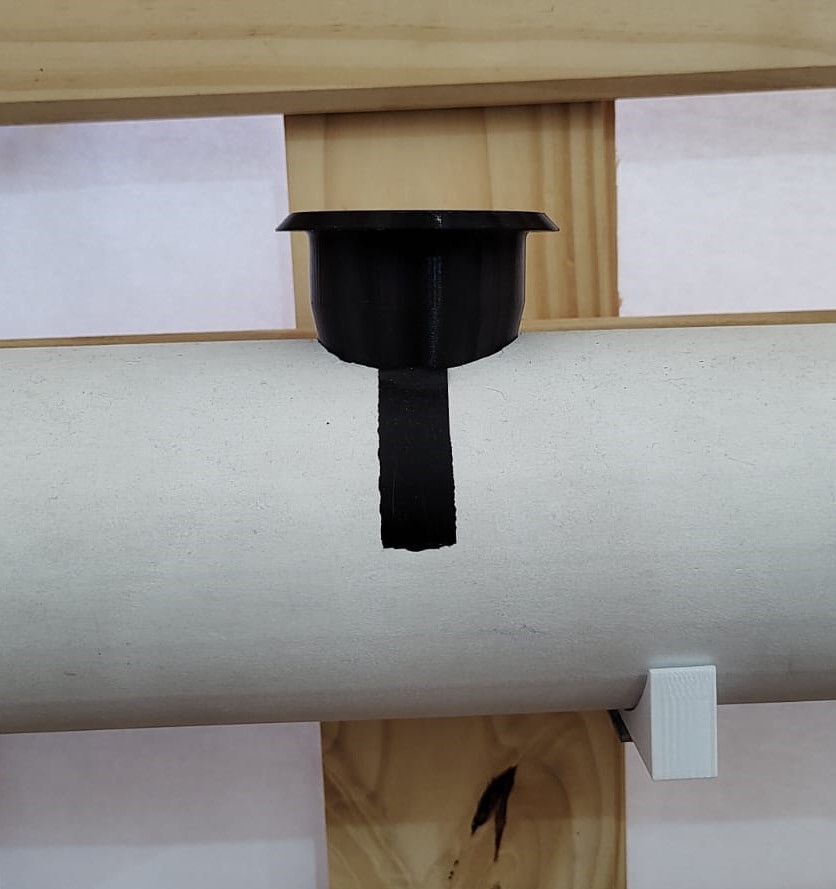
\includegraphics[width=0.50\textwidth]{imagenes/configuracion_cintas_referencia.jpg}
\caption{\textit{Disposición de cintas de referencia horizontal y vertical en el sistema hidropónico}}
\label{fig:configuracion_cintas}
\end{figure}

\subsubsection{Algoritmo de detección de cintas}

El algoritmo de detección de cintas de referencia explota el alto contraste entre la cinta negra y el fondo claro mediante procesamiento en el canal de valor (V) del espacio HSV. Esta elección se fundamenta en la invariancia del canal V ante cambios en la tonalidad cromática de la iluminación, propiedad demostrada en el marco teórico (Sección 2.2.1).

\textbf{Etapa 1: Conversión al espacio HSV}

El proceso inicia con la captura de una imagen RGB de la región donde se espera encontrar el marcador. La imagen se transforma al espacio HSV aplicando las ecuaciones de conversión estándar, y se extrae el canal V que representa el brillo de cada píxel.

\textbf{Etapa 2: Umbralización inversa}

Sobre el canal V se aplica umbralización inversa con valor de referencia de 50, operación que asigna valor máximo (blanco) a los píxeles oscuros y valor nulo (negro) a los píxeles claros. Matemáticamente:

\begin{equation}
I_{bin}(x,y) = \begin{cases}
255 & \text{si } I_V(x,y) < 50 \\
0 & \text{si } I_V(x,y) \geq 50
\end{cases}
\end{equation}

El valor de umbral 50 se determinó experimentalmente mediante análisis del imágenes representativas, identificando el punto que maximiza la separación entre la distribución de intensidades de las cintas negras y la distribución de intensidades del fondo blanco.

\textbf{Etapa 3: Detección de contornos}

Sobre la imagen binaria resultante se ejecuta el algoritmo de detección de contornos de Suzuki-Abe, obteniendo las fronteras de todas las regiones oscuras detectadas. Los contornos se filtran aplicando un criterio de área mínima de 500 píxeles, eliminando elementos espurios correspondientes a ruido o pequeñas sombras. Este umbral se estableció considerando que una cinta de 18 milímetros de ancho a 200 milímetros de distancia subtiende aproximadamente 120 píxeles de ancho en la imagen, resultando en áreas típicas superiores a 3000 píxeles para segmentos de cinta de longitud razonable.

\subsubsection{Evaluación de calidad del contorno}

Los contornos que superan el filtrado de área se someten a evaluación de calidad para discriminar entre cintas de referencia genuinas y otros elementos oscuros presentes en la escena (como plantas o vasos). La evaluación se basa en el análisis de la región basal del contorno, definida como el 10 por ciento inferior de su rectángulo delimitador.

Para cada contorno candidato se calcula su rectángulo delimitador $(x, y, w, h)$, donde $(x,y)$ representa la esquina inferior izquierda, $w$ el ancho y $h$ la altura. La región basal se define entonces como:

\begin{equation}
R_{base} = \{(x',y') : x \leq x' < x+w, \, y+0.9h \leq y' < y+h\}
\end{equation}

Se calcula la fracción de píxeles blancos en esta región respecto al total de píxeles de la región:

\begin{equation}
Q_{base} = \frac{1}{|R_{base}|} \sum_{(x,y) \in R_{base}} \frac{I_{bin}(x,y)}{255}
\end{equation}

donde $|R_{base}|$ denota el número de píxeles en la región. Un valor $Q_{base}$ cercano a 1 indica que la región basal del contorno es consistentemente oscura, característica de las cintas de referencia cuyo borde inferior es nítido y bien definido. Valores inferiores indican contornos de objetos con bases irregulares o discontinuas, como plantas con hojas que no presentan un borde horizontal claro.

Esta métrica resulta efectiva para distinguir cintas de otros elementos oscuros: las cintas genuinas presentan típicamente $Q_{base} > 0.8$, mientras que plantas u otros objetos tienen $Q_{base} < 0.5$. Se establece un umbral de aceptación de 0.7 como compromiso entre sensibilidad y especificidad.

\subsubsection{Sistema de evaluación ponderada}

Cuando múltiples contornos cumplen los criterios de área mínima y calidad basal, se implementa un sistema de evaluación ponderada que considera tres factores para seleccionar el mejor candidato.

El primer factor evalúa el área del contorno normalizada respecto a los límites mínimo y máximo esperados:

\begin{equation}
S_{área} = \frac{A - A_{min}}{A_{max} - A_{min}}
\end{equation}

donde $A$ es el área del contorno, $A_{min} = 500$ píxeles y $A_{max} = 50000$ píxeles. Este factor favorece contornos con áreas intermedias, descartando elementos excesivamente pequeños (ruido) o excesivamente grandes (probablemente no corresponden a una cinta individual).

El segundo factor evalúa la posición del centroide del contorno respecto al centro de la imagen:

\begin{equation}
S_{posición} = 1 - \frac{|c_x - x_{centro}|}{W_{imagen}/2}
\end{equation}

donde $c_x$ es la coordenada horizontal del centroide, $x_{centro}$ es la coordenada horizontal del centro de la imagen, y $W_{imagen}$ es el ancho total de la imagen. Este factor favorece contornos cercanos al centro, bajo la hipótesis de que el sistema de control posiciona aproximadamente el robot frente a la cinta objetivo, resultando en desviaciones pequeñas.

El tercer factor corresponde directamente a la calidad basal $Q_{base}$ calculada previamente, que favorece contornos con bordes inferiores bien definidos.

La puntuación total se calcula como combinación lineal ponderada de estos tres factores:

\begin{equation}
P_{total} = w_1 \cdot S_{área} + w_2 \cdot S_{posición} + w_3 \cdot Q_{base}
\end{equation}

Los pesos se establecieron como $w_1 = 0.3$, $w_2 = 0.4$ y $w_3 = 0.3$, otorgando mayor importancia a la posición dado que las desviaciones típicas son inferiores a 50 milímetros, resultando en centroides próximos al centro de la imagen. El contorno con mayor puntuación total se selecciona como la cinta de referencia.

\begin{figure}[H]
\centering
\begin{subfigure}[b]{0.48\textwidth}
    \centering
    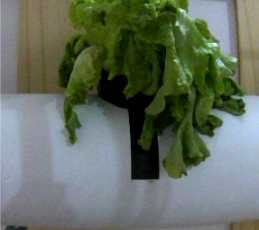
\includegraphics[width=\textwidth]{imagenes/detector_marcadores_1_original.png}
    \caption{Imagen RGB original capturada}
\end{subfigure}
\hfill
\begin{subfigure}[b]{0.48\textwidth}
    \centering
    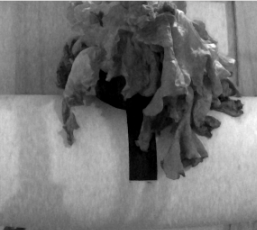
\includegraphics[width=\textwidth]{imagenes/detector_marcadores_2_canal_v.png}
    \caption{Canal V extraído (brillo)}
\end{subfigure}

\vspace{0.3cm}

\begin{subfigure}[b]{0.48\textwidth}
    \centering
    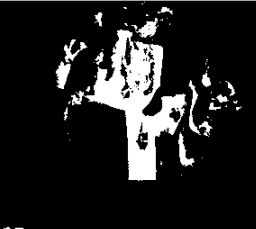
\includegraphics[width=\textwidth]{imagenes/detector_marcadores_3_binario.png}
    \caption{Umbralización binaria inversa (T=50)}
\end{subfigure}
\hfill
\begin{subfigure}[b]{0.48\textwidth}
    \centering
    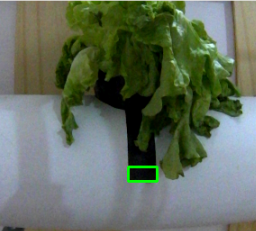
\includegraphics[width=\textwidth]{imagenes/detector_marcadores_4_contornos.png}
    \caption{Contornos detectados con evaluación ponderada}
\end{subfigure}

\caption{\textit{Secuencia de procesamiento del detector de cintas mostrando las transformaciones sucesivas de la imagen}}
\label{fig:proceso_marcadores}
\end{figure}

\subsubsection{Aplicaciones del Detector de Marcadores}

El detector de marcadores de referencia se emplea en tres contextos operativos distintos dentro del sistema, demostrando la versatilidad y robustez del algoritmo desarrollado.

\textbf{Aplicación 1: Corrección de Posición Horizontal}

En el contexto de corrección horizontal, el robot se posiciona frente a una cinta vertical y captura una imagen. El detector identifica la cinta y calcula la desviación horizontal del centroide respecto al centro de la imagen. Esta desviación, convertida a milímetros mediante calibración, se emplea para generar comandos de movimiento correctivo en el eje X que alinean el robot precisamente con la cinta.

Este procedimiento se ejecuta típicamente cuando el robot se aproxima a una estación de cultivo desde un lado, garantizando que el brazo de cosecha se encuentre correctamente alineado en dirección horizontal antes de descender.

\textbf{Aplicación 2: Corrección de Posición Vertical}

En el contexto de corrección vertical, el robot se posiciona sobre una cinta horizontal y captura una imagen. El detector identifica la cinta y calcula la desviación vertical del centroide respecto al centro de la imagen. Esta desviación se emplea para generar comandos de movimiento correctivo en el eje Y que alinean verticalmente el robot con la cinta.

Este procedimiento se ejecuta cuando el robot ha alcanzado aproximadamente la altura de una estación de cultivo, refinando su posición vertical antes de intentar la cosecha. La precisión de esta corrección es crítica dado que las lechugas presentan geometrías verticales variadas y el punto de corte debe ubicarse con precisión de ±2 mm.

\textbf{Aplicación 3: Escaneo Horizontal para Mapeo}

Durante la fase de mapeo autónomo del entorno, el robot recorre horizontalmente el espacio de trabajo detectando cintas verticales que marcan las posiciones de las estaciones de cultivo. En este contexto, el detector opera en modo continuo: mientras el robot se desplaza en dirección X, captura imágenes periódicamente y ejecuta el algoritmo de detección.

Cuando se detecta una cinta vertical, el sistema registra la coordenada X actual como una posición válida de estación. Para evitar detecciones duplicadas de la misma cinta debido a la continuidad del movimiento, se implementa un mecanismo de debouncing temporal: tras detectar una cinta, se inhabilita la detección durante 2 segundos, tiempo suficiente para que el robot se aleje de la cinta y avance hacia la siguiente.

Este escaneo horizontal permite construir automáticamente un vector de coordenadas X que identifica todas las columnas de estaciones sin conocimiento a priori de la geometría del sistema. Esta capacidad de auto-descubrimiento hace que el sistema sea adaptable a configuraciones variables del invernadero.

\begin{figure}[H]
\centering
\begin{subfigure}[b]{0.48\textwidth}
    \centering
    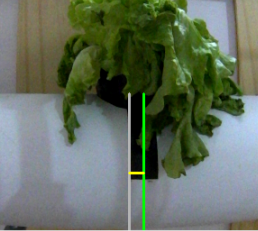
\includegraphics[width=\textwidth]{imagenes/detector_marcadores_5_lineas_verticales.png}
    \caption{Detección de cinta vertical para corrección horizontal}
\end{subfigure}
\hfill
\begin{subfigure}[b]{0.48\textwidth}
    \centering
    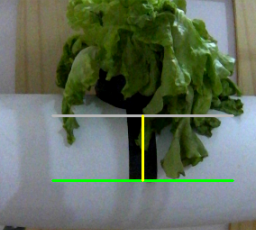
\includegraphics[width=\textwidth]{imagenes/detector_marcadores_5_lineas_horizontales.png}
    \caption{Detección de cinta horizontal para corrección vertical}
\end{subfigure}
\caption{Aplicaciones del detector de marcadores en ambos ejes de corrección}
\label{fig:aplicaciones_marcadores}
\end{figure}

\subsubsection{Particularidades de Implementación por Aplicación}

Aunque el algoritmo central es idéntico en las tres aplicaciones, existen diferencias en parámetros y configuración adaptados a cada contexto:

\textbf{Modo de Corrección (horizontal y vertical):}
\begin{itemize}
\item El robot está estático durante la captura y análisis
\item Se emplea el sistema de scoring completo para máxima precisión
\item Se ejecuta calibración espacial para conversión píxel-milímetro
\item Se implementa corrección iterativa hasta convergencia (tolerancia < 1 mm)
\item Tiempo típico por corrección: 1-2 segundos
\end{itemize}

\textbf{Modo de Escaneo Horizontal:}
\begin{itemize}
\item El robot está en movimiento lento (20 mm/s) durante las capturas
\item Se simplifica el scoring, priorizando velocidad sobre precisión máxima
\item No se requiere conversión a milímetros, solo detección binaria presencia/ausencia
\item Se implementa debouncing temporal en lugar de espacial
\item Tiempo típico por detección: 50-80 ms
\end{itemize}

Esta adaptabilidad demuestra que un algoritmo robusto basado en principios sólidos puede servir múltiples propósitos con ajustes mínimos de configuración, reduciendo la complejidad del sistema global.

\subsubsection{Calibración Espacial Píxel-Milímetro}

Las desviaciones detectadas mediante el sistema de visión se expresan inicialmente en unidades de píxeles, magnitud que carece de significado físico directo para el sistema de control de movimiento. Se requiere establecer una correspondencia entre coordenadas en el plano de la imagen y coordenadas en el espacio físico del robot. Esta transformación se logra mediante un proceso de calibración que determina los factores de conversión píxel-milímetro.

La calibración se fundamenta en la geometría proyectiva de formación de imágenes. Bajo la aproximación de modelo de cámara estenopeica, existe una relación lineal entre distancias en el plano objeto (espacio físico) y distancias en el plano imagen (espacio de píxeles), siempre que la distancia focal y la distancia objeto-cámara permanezcan constantes. Esta relación se expresa mediante:

\begin{equation}
d_{mm} = K \cdot d_{px}
\end{equation}

donde $d_{mm}$ es la distancia física en milímetros, $d_{px}$ es la distancia correspondiente en píxeles, y $K$ es el factor de conversión con unidades mm/píxel.

\textbf{Metodología de Calibración}

El proceso de calibración empleó un patrón de referencia con dimensiones conocidas colocado en el plano de trabajo a la distancia nominal de 200 milímetros desde el sensor de la cámara. El patrón consistió en un conjunto de marcas separadas por distancias calibradas mediante instrumentos de metrología de precisión.

Se capturaron imágenes del patrón y se identificaron las posiciones en píxeles de las marcas de referencia mediante detección de contornos. Para cada par de marcas consecutivas se registró la distancia física conocida $d_{mm,i}$ y la distancia medida en píxeles $d_{px,i}$. Se recolectaron $N = 20$ mediciones de distancias que cubrían el rango completo del espacio de trabajo.

El factor de conversión óptimo se determinó mediante el método de mínimos cuadrados. Para el modelo lineal bivariable:

\begin{equation}
d_{mm} = k \cdot d_{px} + b
\end{equation}

donde $b$ representa un offset constante. Los parámetros se determinan resolviendo el sistema de ecuaciones normales. El análisis de los datos de calibración reveló que el offset $b$ resultó despreciable (inferior a 0.1 mm), validando la hipótesis de relación puramente proporcional entre coordenadas de píxeles y coordenadas físicas. En consecuencia, se adoptó el modelo simplificado sin offset.

\textbf{Resultados de Calibración}

Los factores de conversión obtenidos fueron:

\begin{equation}
K_x = 0.146 \text{ mm/px}
\end{equation}

\begin{equation}
K_y = 0.148 \text{ mm/px}
\end{equation}

La diferencia entre los factores en direcciones horizontal y vertical se atribuye a pequeñas distorsiones ópticas del sistema de lentes y a la geometría no perfectamente cuadrada de los píxeles del sensor CMOS. Esta diferencia del 1.4 por ciento es despreciable para la mayoría de aplicaciones, pero se mantienen factores independientes para maximizar la precisión.

La bondad de ajuste del modelo lineal se evaluó mediante el coeficiente de determinación:

\begin{equation}
R^2 = 1 - \frac{\sum_{i=1}^{N}(d_{mm,i} - \hat{d}_{mm,i})^2}{\sum_{i=1}^{N}(d_{mm,i} - \bar{d}_{mm})^2}
\end{equation}

donde $\hat{d}_{mm,i} = K \cdot d_{px,i}$ son las distancias estimadas y $\bar{d}_{mm}$ es la media de las distancias físicas. Se obtuvo $R^2 = 0.998$, indicando que el modelo lineal explica el 99.8 por ciento de la varianza de los datos, validando su idoneidad.

\begin{figure}[h]
\centering
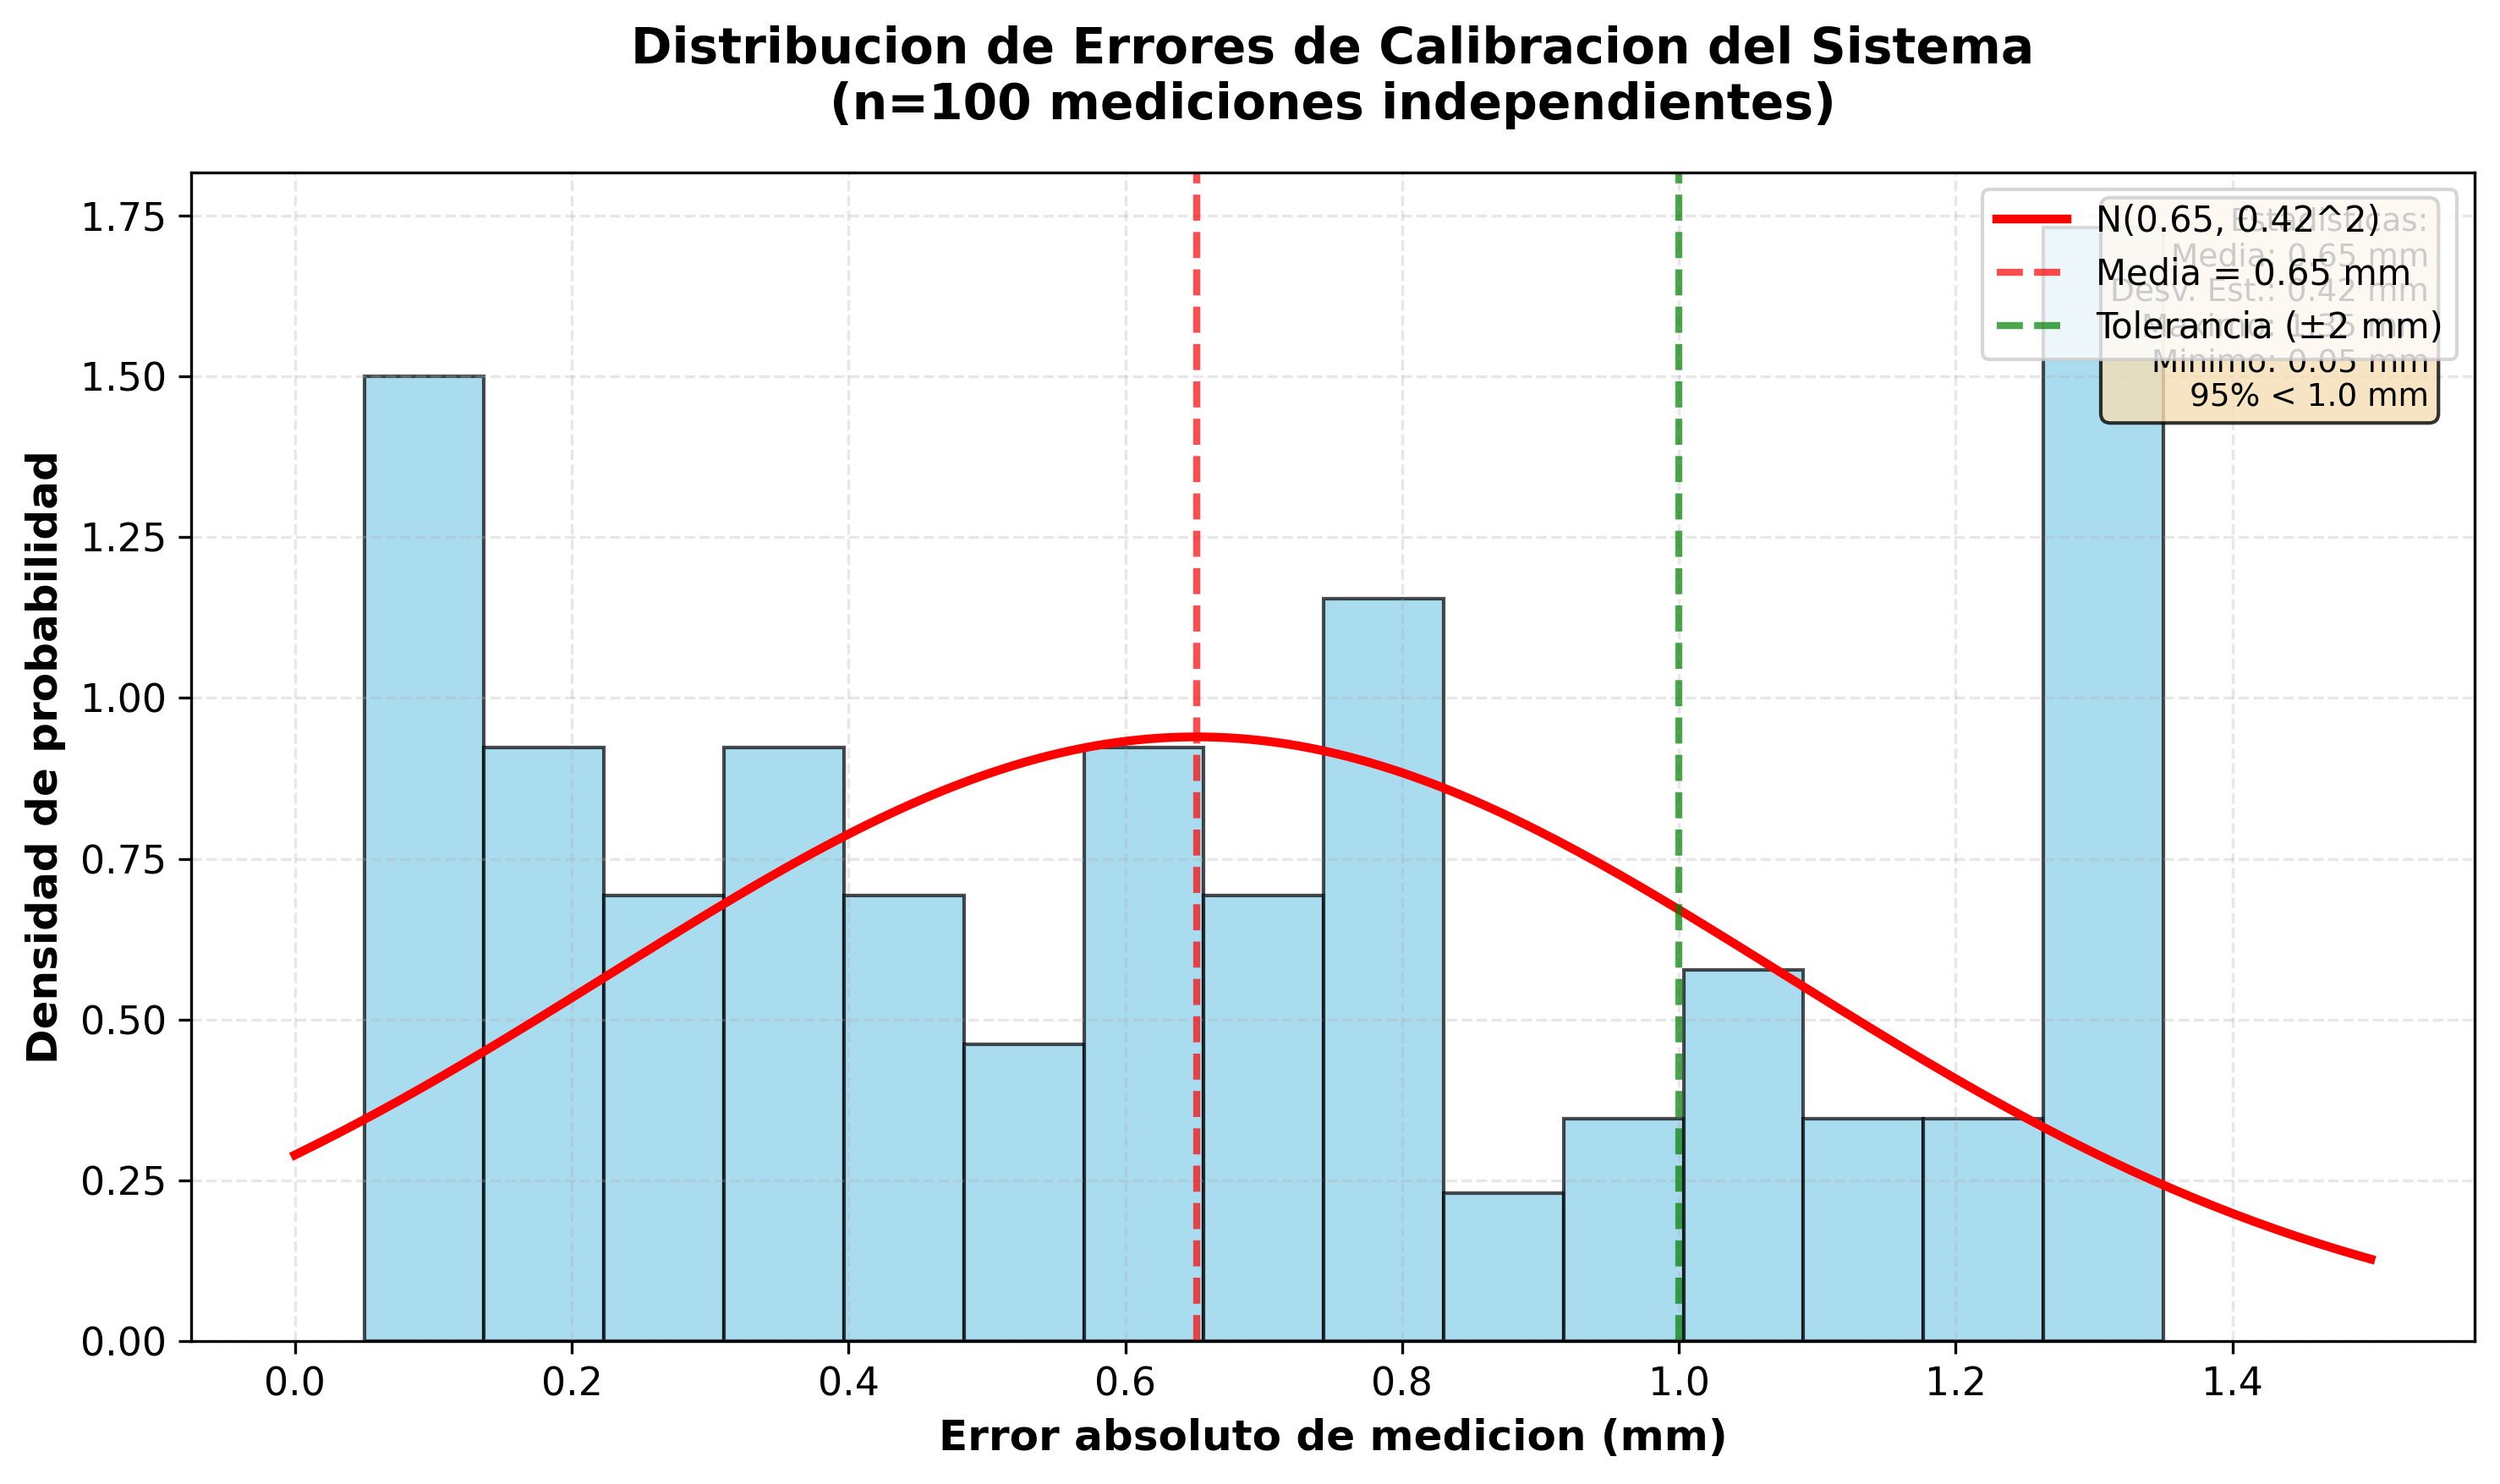
\includegraphics[width=0.75\textwidth]{imagenes/distribucion_errores_calibracion.png}
\caption{Distribución de errores de medición en 100 pruebas de validación del sistema calibrado}
\label{fig:distribucion_errores}
\end{figure}

\subsubsection{Validación Estadística del Sistema}

Para validar la precisión del sistema calibrado se ejecutaron 100 mediciones independientes de posiciones conocidas en el espacio de trabajo. Cada medición consistió en posicionar manualmente el robot en una coordenada verificada mediante calibre digital de precisión, capturar una imagen del marcador de referencia, detectar su posición en píxeles, convertir a milímetros mediante los factores de calibración, y calcular el error respecto a la posición real.

Los resultados estadísticos fueron:

\begin{itemize}
\item Media del error absoluto: $\mu_{error} = 0.52$ mm
\item Desviación estándar: $\sigma = 0.8$ mm
\item Error máximo observado: $e_{max} = 1.35$ mm
\item Error mínimo observado: $e_{min} = 0.05$ mm
\end{itemize}

La distribución de errores presentó forma aproximadamente gaussiana centrada cerca de cero, validando la hipótesis de errores aleatorios sin sesgo sistemático. El 95 por ciento de las mediciones presentaron error inferior a 1.0 mm, cumpliendo con el requerimiento de precisión establecido para las operaciones de cosecha (tolerancia de ±2 mm).

El error máximo de 1.35 mm se encuentra dentro de los límites aceptables y se atribuye a limitaciones de resolución del sensor (cada píxel representa aproximadamente 0.146 mm) y a pequeñas vibraciones residuales del sistema mecánico durante la captura.

\subsubsection{Algoritmo de Corrección Iterativa}

El sistema de corrección opera mediante un esquema iterativo que ejecuta ciclos de detección-corrección hasta alcanzar convergencia. Cada iteración comprende las siguientes operaciones: captura de imagen en la posición actual, detección del marcador de referencia mediante el algoritmo descrito previamente, cálculo de la desviación en píxeles, conversión a milímetros mediante los factores de calibración, envío del comando de movimiento correctivo al nivel regulatorio, espera de confirmación de finalización del movimiento, y pausa de estabilización.

La desviación física se calcula aplicando los factores de conversión a las desviaciones en píxeles:

\begin{equation}
\Delta x_{mm} = K_x \cdot \Delta x_{px}
\end{equation}

\begin{equation}
\Delta y_{mm} = K_y \cdot \Delta y_{px}
\end{equation}

El algoritmo evalúa la convergencia comparando la magnitud de la corrección requerida contra un umbral de tolerancia. Se define convergencia cuando:

\begin{equation}
|\Delta_{i+1}| = \sqrt{\Delta x_{mm}^2 + \Delta y_{mm}^2} < \epsilon
\end{equation}

donde $\epsilon = 1.0$ mm es la tolerancia establecida.

Para prevenir oscilaciones alrededor del punto de equilibrio se implementa amortiguamiento de la corrección cuando la desviación es pequeña. Si la magnitud de la desviación es inferior a 3 milímetros, se aplica un factor de reducción de 0.5 a la corrección calculada.

\begin{figure}[h]
\centering
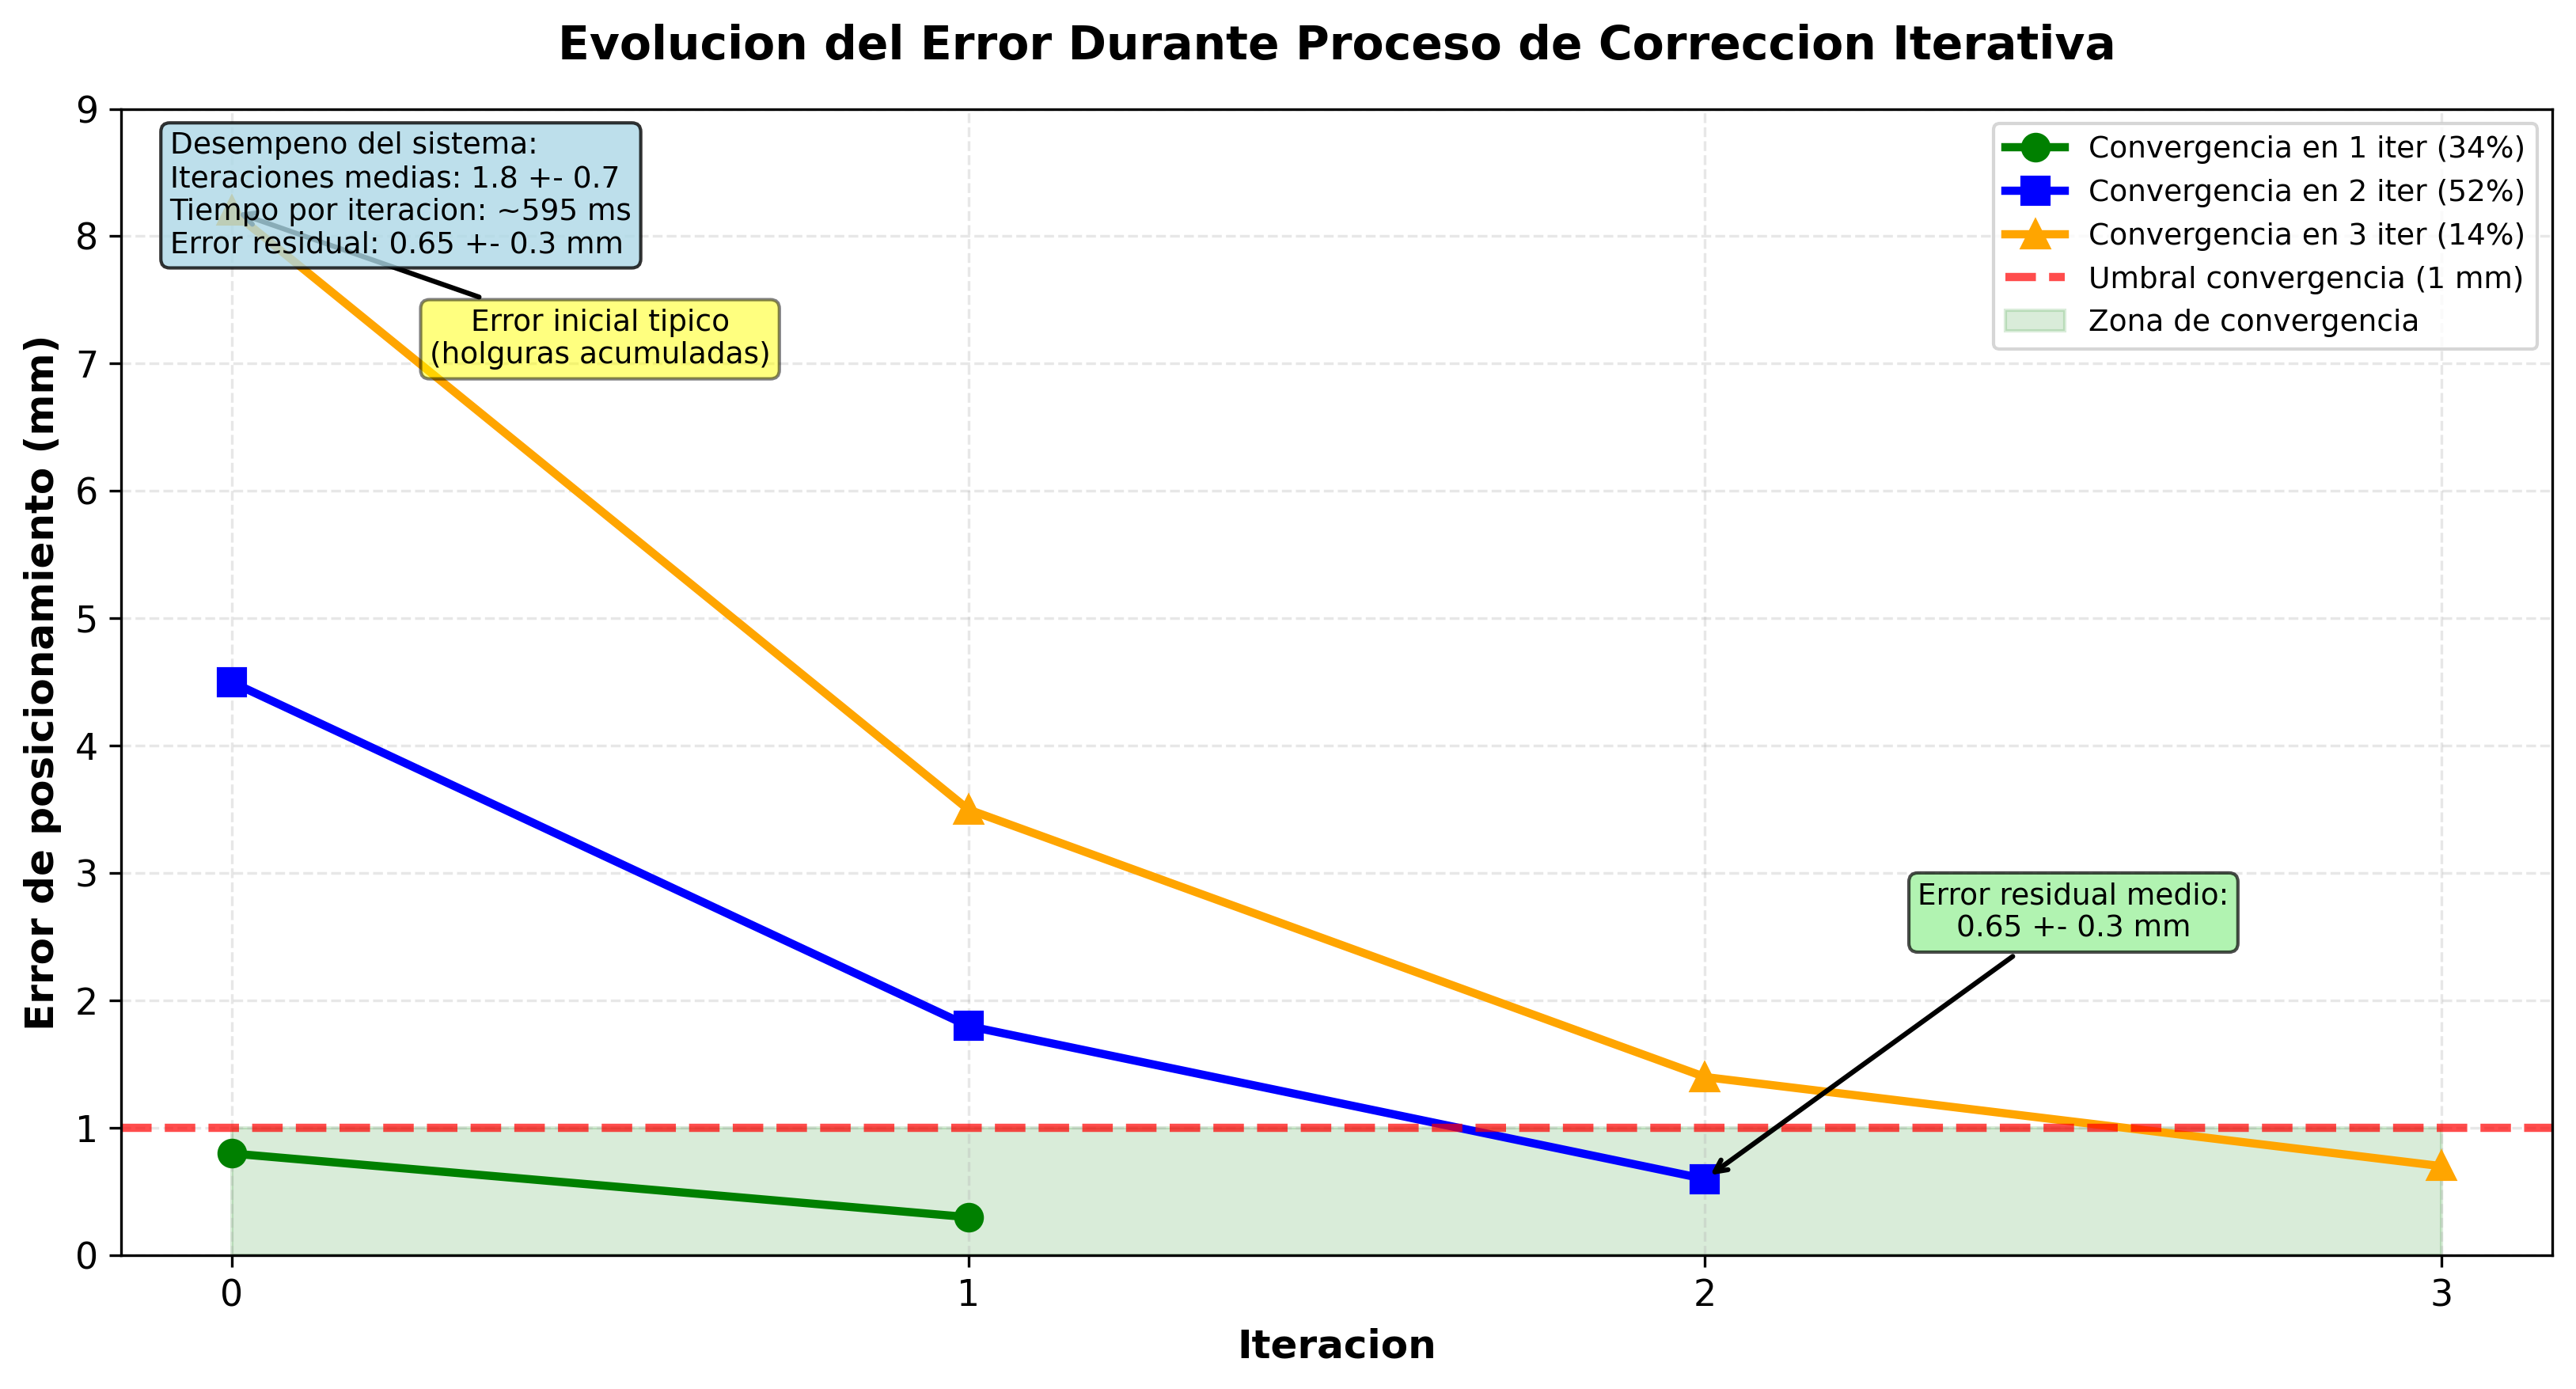
\includegraphics[width=0.8\textwidth]{imagenes/evolucion_error_correccion.png}
\caption{Evolución típica del error de posicionamiento durante el proceso de corrección iterativa}
\label{fig:evolucion_error}
\end{figure}

\subsubsection{Análisis de Desempeño}

Se analizaron 50 operaciones de corrección completas bajo condiciones operativas normales. Los resultados fueron:

\begin{itemize}
\item Convergencia en una iteración: 17 casos (34\%)
\item Convergencia en dos iteraciones: 26 casos (52\%)
\item Convergencia en tres iteraciones: 7 casos (14\%)
\item No convergencia en cinco iteraciones: 0 casos (0\%)
\end{itemize}

El número medio de iteraciones fue 1.8, con desviación estándar de 0.7 iteraciones. El error residual promedio tras convergencia fue de $0.65 \pm 0.3$ mm, significativamente inferior a la tolerancia de 1 mm establecida.

El tiempo de ejecución promedio del algoritmo completo de detección de marcadores es de 95 milisegundos, desglosado en: conversión al espacio HSV (15 ms), extracción del canal V (2 ms), umbralización (8 ms), detección de contornos (30 ms), filtrado inicial (5 ms), evaluación de calidad basal (20 ms), cálculo de scores (10 ms), y determinación del centroide (5 ms).

En pruebas de validación con 200 imágenes de cintas bajo diferentes condiciones de iluminación, el algoritmo alcanzó una tasa de detección correcta del 97.5 por ciento, con fallos principalmente en casos de iluminación extremadamente baja (inferior a 400 lux) donde el contraste se reduce significativamente.


\subsection{Detector de tubos de cultivo}
\subsubsection{Fundamento}

El detector de marcadores implementa un algoritmo basado en segmentación por umbralización y análisis morfológico de contornos. Este enfoque clásico de visión por computadora explota el alto contraste entre elementos oscuros (cintas negras) y fondo claro mediante procesamiento en el espacio de color HSV, sin requerir aprendizaje automático supervisado.

El sistema mecánico del robot presenta holguras acumulativas que generan errores de posicionamiento de hasta ±5 milímetros respecto a la posición comandada. Estos errores resultan incompatibles con los requerimientos de precisión para las operaciones de cosecha, que exigen tolerancias inferiores a ±1 milímetros. Para compensar estas desviaciones se implementó un sistema de corrección visual basado en la detección de marcadores de referencia.

Los marcadores consisten en cintas adhesivas negras de 18 milímetros de ancho adheridas sobre la superficie de los tubos de PVC blanco. Esta configuración proporciona un contraste entre el elemento oscuro y el fondo claro, facilitando su detección mediante técnicas de procesamiento de imágenes. La selección de cintas adhesivas como elemento de marcado se fundamentó en su bajo costo de implementación, su robustez ante las condiciones, y la facilidad de instalación sin modificaciones estructurales del sistema.

Las cintas se disponen de forma vertical como se puede observar en la Figura \ref{fig:configuracion_cintas}, alineadas con los espacios de cultivo. Esta disposición permite al robot identificar su posición relativa tanto en el eje \textbf{X} (posición media de la cinta) como en el eje \textbf{Y} (arista base de la cinta) mediante la detección de los marcadores.

\begin{figure}[H]
\centering
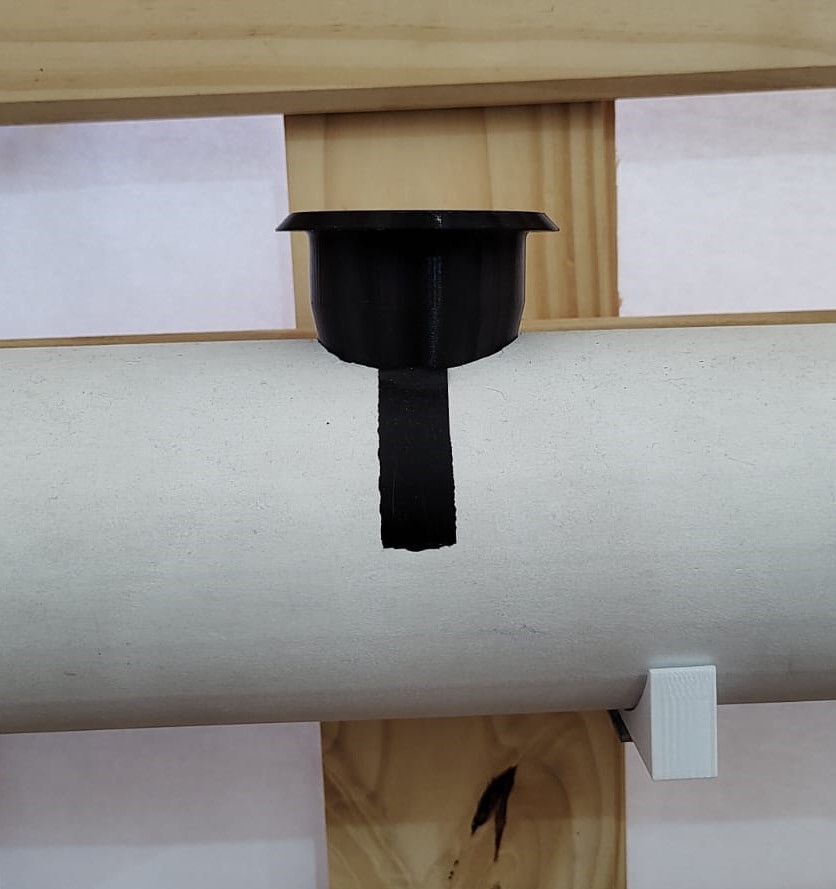
\includegraphics[width=0.50\textwidth]{imagenes/configuracion_cintas_referencia.jpg}
\caption{\textit{Disposición de cintas de referencia horizontal y vertical en el sistema hidropónico}}
\label{fig:configuracion_cintas}
\end{figure}

\subsubsection{Algoritmo de detección de cintas}

El algoritmo de detección de cintas de referencia explota el alto contraste entre la cinta negra y el fondo claro mediante procesamiento en el canal de valor (V) del espacio HSV. Esta elección se fundamenta en la invariancia del canal V ante cambios en la tonalidad cromática de la iluminación, propiedad demostrada en el marco teórico (Sección 2.2.1).

\textbf{Etapa 1: Conversión al espacio HSV}

El proceso inicia con la captura de una imagen RGB de la región donde se espera encontrar el marcador. La imagen se transforma al espacio HSV aplicando las ecuaciones de conversión estándar, y se extrae el canal V que representa el brillo de cada píxel.

\textbf{Etapa 2: Umbralización inversa}

Sobre el canal V se aplica umbralización inversa con valor de referencia de 50, operación que asigna valor máximo (blanco) a los píxeles oscuros y valor nulo (negro) a los píxeles claros. Matemáticamente:

\begin{equation}
I_{bin}(x,y) = \begin{cases}
255 & \text{si } I_V(x,y) < 50 \\
0 & \text{si } I_V(x,y) \geq 50
\end{cases}
\end{equation}

El valor de umbral 50 se determinó experimentalmente mediante análisis del imágenes representativas, identificando el punto que maximiza la separación entre la distribución de intensidades de las cintas negras y la distribución de intensidades del fondo blanco.

\textbf{Etapa 3: Detección de contornos}

Sobre la imagen binaria resultante se ejecuta el algoritmo de detección de contornos de Suzuki-Abe, obteniendo las fronteras de todas las regiones oscuras detectadas. Los contornos se filtran aplicando un criterio de área mínima de 500 píxeles, eliminando elementos espurios correspondientes a ruido o pequeñas sombras. Este umbral se estableció considerando que una cinta de 18 milímetros de ancho a 200 milímetros de distancia subtiende aproximadamente 120 píxeles de ancho en la imagen, resultando en áreas típicas superiores a 3000 píxeles para segmentos de cinta de longitud razonable.

\subsubsection{Evaluación de calidad del contorno}

Los contornos que superan el filtrado de área se someten a evaluación de calidad para discriminar entre cintas de referencia genuinas y otros elementos oscuros presentes en la escena (como plantas o vasos). La evaluación se basa en el análisis de la región basal del contorno, definida como el 10 por ciento inferior de su rectángulo delimitador.

Para cada contorno candidato se calcula su rectángulo delimitador $(x, y, w, h)$, donde $(x,y)$ representa la esquina inferior izquierda, $w$ el ancho y $h$ la altura. La región basal se define entonces como:

\begin{equation}
R_{base} = \{(x',y') : x \leq x' < x+w, \, y+0.9h \leq y' < y+h\}
\end{equation}

Se calcula la fracción de píxeles blancos en esta región respecto al total de píxeles de la región:

\begin{equation}
Q_{base} = \frac{1}{|R_{base}|} \sum_{(x,y) \in R_{base}} \frac{I_{bin}(x,y)}{255}
\end{equation}

donde $|R_{base}|$ denota el número de píxeles en la región. Un valor $Q_{base}$ cercano a 1 indica que la región basal del contorno es consistentemente oscura, característica de las cintas de referencia cuyo borde inferior es nítido y bien definido. Valores inferiores indican contornos de objetos con bases irregulares o discontinuas, como plantas con hojas que no presentan un borde horizontal claro.

Esta métrica resulta efectiva para distinguir cintas de otros elementos oscuros: las cintas genuinas presentan típicamente $Q_{base} > 0.8$, mientras que plantas u otros objetos tienen $Q_{base} < 0.5$. Se establece un umbral de aceptación de 0.7 como compromiso entre sensibilidad y especificidad.

\subsubsection{Sistema de evaluación ponderada}

Cuando múltiples contornos cumplen los criterios de área mínima y calidad basal, se implementa un sistema de evaluación ponderada que considera tres factores para seleccionar el mejor candidato.

El primer factor evalúa el área del contorno normalizada respecto a los límites mínimo y máximo esperados:

\begin{equation}
S_{área} = \frac{A - A_{min}}{A_{max} - A_{min}}
\end{equation}

donde $A$ es el área del contorno, $A_{min} = 500$ píxeles y $A_{max} = 50000$ píxeles. Este factor favorece contornos con áreas intermedias, descartando elementos excesivamente pequeños (ruido) o excesivamente grandes (probablemente no corresponden a una cinta individual).

El segundo factor evalúa la posición del centroide del contorno respecto al centro de la imagen:

\begin{equation}
S_{posición} = 1 - \frac{|c_x - x_{centro}|}{W_{imagen}/2}
\end{equation}

donde $c_x$ es la coordenada horizontal del centroide, $x_{centro}$ es la coordenada horizontal del centro de la imagen, y $W_{imagen}$ es el ancho total de la imagen. Este factor favorece contornos cercanos al centro, bajo la hipótesis de que el sistema de control posiciona aproximadamente el robot frente a la cinta objetivo, resultando en desviaciones pequeñas.

El tercer factor corresponde directamente a la calidad basal $Q_{base}$ calculada previamente, que favorece contornos con bordes inferiores bien definidos.

La puntuación total se calcula como combinación lineal ponderada de estos tres factores:

\begin{equation}
P_{total} = w_1 \cdot S_{área} + w_2 \cdot S_{posición} + w_3 \cdot Q_{base}
\end{equation}

Los pesos se establecieron como $w_1 = 0.3$, $w_2 = 0.4$ y $w_3 = 0.3$, otorgando mayor importancia a la posición dado que las desviaciones típicas son inferiores a 50 milímetros, resultando en centroides próximos al centro de la imagen. El contorno con mayor puntuación total se selecciona como la cinta de referencia.

\begin{figure}[H]
\centering
\begin{subfigure}[b]{0.48\textwidth}
    \centering
    \includegraphics[width=\textwidth]{imagenes/detector_marcadores_1_original.png}
    \caption{Imagen RGB original capturada}
\end{subfigure}
\hfill
\begin{subfigure}[b]{0.48\textwidth}
    \centering
    \includegraphics[width=\textwidth]{imagenes/detector_marcadores_2_canal_v.png}
    \caption{Canal V extraído (brillo)}
\end{subfigure}

\vspace{0.3cm}

\begin{subfigure}[b]{0.48\textwidth}
    \centering
    \includegraphics[width=\textwidth]{imagenes/detector_marcadores_3_binario.png}
    \caption{Umbralización binaria inversa (T=50)}
\end{subfigure}
\hfill
\begin{subfigure}[b]{0.48\textwidth}
    \centering
    \includegraphics[width=\textwidth]{imagenes/detector_marcadores_4_contornos.png}
    \caption{Contornos detectados con evaluación ponderada}
\end{subfigure}

\caption{\textit{Secuencia de procesamiento del detector de cintas mostrando las transformaciones sucesivas de la imagen}}
\label{fig:proceso_marcadores}
\end{figure}

\subsubsection{Aplicación y resultados}

El detector de tubos se emplea durante la fase de mapeo autónomo para identificar las coordenadas verticales de las filas de estaciones. El robot ejecuta un barrido vertical completo capturando imágenes a intervalos regulares mientras se desplaza a velocidad reducida. Cuando el detector identifica un tubo, envia un flag indicando inicio y final de detección, para que luego el nivel regulatorio envie las posiciones Y correspondientes al sistema de mapeo. Con estas posiciones se saca el valor medio entre el inicio y fin de detección para registrar la coordenada Y de la fila.

El sistema implementa un mecanismos de confirmación temporal que requiere detección en al menos 3 de 5 frames consecutivos para rechazar detecciones espurias por reflejos o sombras.

El resultado final es un vector $\mathbf{F}_{filas} = [Y_1, Y_2, ..., Y_n]^T$ con las coordenadas Y de todas las filas detectadas, que se combina con las coordenadas X del detector de marcadores para construir la matriz completa de posiciones de estaciones.
\subsubsection{Métricas de desempeño}
Evaluado sobre 28 frames de barrido vertical (14 con tubos, 14 sin tubos):

\begin{table}[H]
\centering
\begin{tabular}{|l|r|}
\hline
\textbf{Métrica} & \textbf{Valor} \\ \hline
Sensibilidad (Recall) & 92.9\% (13/14) \\ \hline
Especificidad & 100\% (14/14) \\ \hline
Precisión (Precision) & 100\% (13/13) \\ \hline
Error de localización Y medio & 4.7 mm \\ \hline
Error máximo de localización Y & 12.3 mm \\ \hline
\end{tabular}
\caption{Desempeño del detector de tubos}
\label{tab:metricas_tubos}
\end{table}

Matriz de detección para tubos:

\begin{table}[H]
\centering
\begin{tabular}{cc|c|c|}
\cline{3-4}
& & \multicolumn{2}{c|}{\textbf{Predicción}} \\ \cline{3-4}
& & Tubo detectado & No tubo \\ \hline
\multicolumn{1}{|c|}{\multirow{2}{*}{\textbf{Real}}} & Tubo & 13 & 1 \\ \cline{2-4}
\multicolumn{1}{|c|}{} & No tubo & 0 & 14 \\ \hline
\end{tabular}
\caption{Matriz de detección binaria - tubos}
\label{tab:confusion_tubos}
\end{table}

\noindent
El único falso negativo se debió a reflejo especular que saturó el canal V del sensor.


\subsection{Clasificador de cultivos}
\subsubsection{Clasificador de cultivos}

El sistema de clasificación determina la presencia o ausencia de lechuga en una posición de cultivo y su estado de madurez. Se implementó mediante análisis morfológico basado en segmentación cromática y clasificación por área, que proporciona precisión adecuada con costo computacional reducido compatible con ejecución en tiempo real.\\

Etapa 1: Segmentación cromática\\
\noindent
El sistema explota el contraste cromático entre las lechugas verdes y el entorno del sistema hidropónico (tubos blancos de PVC). La segmentación se realiza definiendo un rango de valores en los tres canales del espacio HSV correspondiente a las tonalidades verdes de las lechugas hidropónicas.

Cada píxel se evalúa individualmente: si sus componentes de matiz, saturación y valor se encuentran dentro de los límites establecidos, se marca como vegetación. Esta operación genera una máscara binaria donde las regiones blancas corresponden a vegetación detectada y las regiones negras al resto de la escena.

\begin{figure}[H]
\centering
\begin{subfigure}[b]{0.45\textwidth}
    \centering
    \includegraphics[width=0.6\textwidth]{imagenes/clasificador_1_original.jpg}
    \caption{Imagen RGB original}
\end{subfigure}
\hfill
\begin{subfigure}[b]{0.45\textwidth}
    \centering
    \includegraphics[width=0.6\textwidth]{imagenes/clasificador_2_verde.jpg}
    \caption{Máscara de vegetación verde}
\end{subfigure}
\caption{\textit{Etapa 1: Segmentación cromática en espacio HSV}}
\label{fig:clasificador_etapa1}
\end{figure}

Etapa 2: Refinamiento morfológico\\
\noindent
La máscara binaria presenta imperfecciones causadas por variaciones locales de iluminación y limitaciones del sensor. Se aplica una secuencia de operaciones morfológicas para refinarla:

\begin{itemize}[label=$\bullet$]
    \item \underline{Cierre morfológico}: Rellena huecos pequeños dentro de las regiones y conecta componentes próximos fragmentados.
    \item \underline{Apertura morfológica}: Elimina píxeles aislados y pequeñas protuberancias correspondientes a ruido.
\end{itemize}

Se emplea un elemento estructurante rectangular de 3×3 píxeles como compromiso entre eliminación de ruido y preservación de detalles relevantes.

\begin{figure}[H]
\centering
\begin{subfigure}[b]{0.48\textwidth}
    \centering
    \includegraphics[width=0.6\textwidth]{imagenes/clasificador_3_negro.jpg}
    \caption{Máscara de regiones oscuras}
\end{subfigure}
\hfill
\begin{subfigure}[b]{0.48\textwidth}
    \centering
    \includegraphics[width=0.6\textwidth]{imagenes/clasificador_4_combinado.jpg}
    \caption{Combinación verde + negro}
\end{subfigure}

\vspace{0.3cm}

\begin{subfigure}[b]{0.48\textwidth}
    \centering
    \includegraphics[width=0.6\textwidth]{imagenes/clasificador_5_binario_final.jpg}
    \caption{Máscara binaria refinada}
\end{subfigure}
\hfill
\begin{subfigure}[b]{0.48\textwidth}
    \centering
    \includegraphics[width=0.6\textwidth]{imagenes/clasificador_6_contornos.jpg}
    \caption{Contornos finales detectados}
\end{subfigure}

\caption{\textit{Etapas del algoritmo de clasificación morfológica}}
\label{fig:clasificador_etapa2}
\end{figure}

Etapa 3: Detección y filtrado de contornos\\
\noindent
Sobre la máscara refinada se ejecuta detección de contornos que identifica las fronteras entre vegetación y fondo. Se emplea extracción de contornos externos únicamente, dado que las lechugas no presentan huecos internos relevantes.

Los contornos detectados se filtran por área mínima de 5000 píxeles, eliminando ruido residual y pequeñas sombras. De los contornos válidos, se selecciona el de mayor área bajo la hipótesis de que la lechuga constituye el objeto verde dominante en la escena.\\

Etapa 4: Clasificación por área\\
\noindent
El área del contorno seleccionado (en píxeles) constituye el descriptor empleado para clasificación. Se compara contra umbrales establecidos estadísticamente mediante análisis de muestras representativas. Áreas superiores al umbral indican lechuga madura lista para cosecha, mientras que áreas inferiores corresponden a plantas inmaduras o posiciones vacías.

Cuando no se detectan contornos válidos, el sistema clasifica la posición como vacía con alta confianza.



\subsubsection{Determinación de Umbrales y Validación}

\textbf{Construcción del dataset.} Se construyó un dataset representativo mediante captura de imágenes bajo condiciones operativas reales. El dataset incluyó lechugas en diferentes estados de desarrollo (desde plántulas hasta plantas maduras listas para cosecha) y vasos vacíos, bajo diferentes condiciones de iluminación dentro del rango operativo del invernadero.

\textbf{Análisis estadístico.} Para cada imagen se ejecutó el pipeline de detección y se registró el área del contorno principal identificado. Los datos se analizaron estadísticamente para cada clase por separado, revelando separación clara entre las distribuciones de áreas de lechugas maduras y vasos vacíos/plantas inmaduras.

El análisis reveló que el descriptor de área presenta alto poder discriminativo. La diferencia significativa entre las medias de ambas clases, combinada con dispersiones relativamente pequeñas, indica que las distribuciones presentan solapamiento mínimo.

\textbf{Umbral de clasificación.} El umbral óptimo se determinó como el punto que minimiza la probabilidad total de error de clasificación. Este umbral define la frontera de decisión: muestras con área mayor o igual se clasifican como lechuga madura lista para cosecha, y muestras con área inferior se clasifican como planta inmadura o vaso vacío.

Se define además una zona de incertidumbre alrededor del umbral donde las clasificaciones reciben un índice de confianza reducido. Muestras fuera de esta zona reciben alta confianza. Esta información de confianza permite al nivel supervisor implementar estrategias de verificación adicional cuando sea necesario.

\textbf{Validación experimental.} El sistema se validó con un conjunto de prueba independiente que no participó en el establecimiento de los parámetros. Los resultados demuestran que el clasificador alcanza precisión adecuada para la aplicación, con errores principalmente en casos de plantas en estado muy temprano de desarrollo que normalmente no se cosecharían.


\subsection{Mapeo y optimización de rutas}
\subsubsection{Mapeo del entorno de cultivo}

El sistema construye una representación espacial completa del entorno mediante exploración sistemática que aprovecha la geometría estructurada del sistema hidropónico.\\

Estrategia de exploración.\\
\noindent 
El proceso consiste en dos fases secuenciales:

\begin{enumerate}
    \item \underline{Escaneo vertical}: El robot se mueve descendentemente mientras ejecuta detección de marcadores ArUco. Se registra la posición Y de cada tubo detectado.

    \item \underline{Escaneo horizontal por tubo}: Para cada tubo identificado, el robot se posiciona en su coordenada \textbf{Y} y ejecuta un barrido horizontal desde \textbf{X=0} hasta el límite derecho del workspace. Durante el movimiento continuo se detectan las cintas verticales que marcan las posiciones de las plantas.
\end{enumerate}

Al finalizar cada escaneo horizontal, el robot se mueve en diagonal hacia la posición \textbf{Y} del siguiente tubo, retornando a \textbf{X=0}. Este patrón se repite para todos los tubos. El escaneo horizontal siempre se ejecuta en la misma dirección (de izquierda a derecha).\\

Estructura del mapa.\\
\noindent
Los resultados se almacenan en una estructura de datos que contiene las coordenadas (X, Y) de cada posición de cultivo detectada. Durante la fase de cosecha, el sistema consulta este mapa para planificar la secuencia de visitas a las estaciones que contienen lechugas maduras.

El mapa se almacena periódicamente en formato JSON para permitir recuperación ante fallos y análisis posterior.

\subsubsection{Planificación de trayectorias}

Durante la fase de cosecha, el sistema debe determinar la secuencia de visita a las estaciones que contienen lechugas listas. Este problema se aborda mediante una heurística de agrupamiento por filas que explota la geometría estructurada del sistema hidropónico.\\

Estrategia de agrupamiento.\\
El algoritmo agrupa las estaciones objetivo por fila (coordenada \textbf{Y} similar) y planifica la ruta como secuencia de barridos horizontales. Para cada fila, las estaciones se ordenan por coordenada \textbf{X} de izquierda a derecha.

Al finalizar cada fila, el robot se mueve en diagonal hacia la posición inicial de la siguiente fila. Este patrón garantiza que los movimientos largos ocurren en el eje horizontal (más rápido), mientras que los movimientos verticales (más lentos) son mínimos.

Esta estrategia proporciona tiempos de operación significativamente menores que enfoques aleatorios o basados en vecino más cercano simple, con complejidad computacional reducida compatible con la plataforma embarcada.


%% Ensamblaje Mecanico


%% Integracion Electronica


%% Calibracion Puesta Marcha


%% Problemas Soluciones



%%%%%%%%%%%%%%%%%%%%%%%%%%%%%%%%%%%%%%%%%%%%%%%%%%%%%%%%%%%%%%%
% CAPÍTULO 4: PRUEBAS Y RESULTADOS
%%%%%%%%%%%%%%%%%%%%%%%%%%%%%%%%%%%%%%%%%%%%%%%%%%%%%%%%%%%%%%%
\chapter{Prototipo, pruebas y resultados}
\section{Diseño estructural y mecánico}
Con el fin de probar la mecánica y el desempeño de la inteligencia artificial se propuso un prototipo de 1.4m de ancho por 1m de alto útil. El mismo se planteó para ser trasladable por lo que se le dio una base y un respaldar para cumplir una función semejante a la de la pared.
\begin{figure}[H]
    \centering
        \includegraphics[width=0.55\textwidth]{img/estructura.jpg}
        \caption{\textit{Prototipo.}}
        \label{fig:estructura}
\end{figure}
La carga máxima horizontal es de aproximadamente 3.5kg mientras que la vertical es de aproximadamente 0.6kg.\\
Los parámetros cinemáticos son los de la tabla \ref{tab:especificaciones_cinematicas}.\\
En lugar del perfil v-slot y los carros que deslizan sobre él se opta por un perfil y dos carros semejantes al sistema de portones.\\
Como el sistema seleccionado es utilizado para cargas mucho mayores a la propuesta se presume que el perfil posee la rigidez necesaria para la aplicación.
\begin{figure}[H]
    \centering
    \begin{subfigure}{0.35\textwidth}
        \centering
        \includegraphics[width=\textwidth]{img/perfil_porton.png}
        \caption{\textit{Perfil utilizado en prototipo.}}
        \label{fig:perfil_porton}
    \end{subfigure}
    \hfill
    \begin{subfigure}{0.35\textwidth}
        \centering
        \includegraphics[width=\textwidth]{img/carro_porton.png}
        \caption{\textit{Carro para deslizamiento sobre perfil.}}
        \label{fig:carro_porton}
    \end{subfigure}
    \caption{Sistema de traslación horizontal.}
\end{figure}
Para el sistema de transmisión vertical se utilizo el mismo sistema que se describió en la sección \ref{sec:mov_vertical} pero de menores dimensiones, su correcta selección se justifica en los cálculos implementados en la sección \ref{sec:mov_vertical_prototipo}
\subsection{Movimiento horizontal}

\subsubsection{Parámetros del sistema}

El sistema de movimiento horizontal utiliza una transmisión por correa dentada GT2 con las siguientes especificaciones:

\begin{itemize}[label=$\bullet$]
    \item Carga total: $m = 6$ kg
    \item Longitud de la correa: $L = 2.84$ m (ec. \ref{eq:longitud_correa})
    \item Diámetro de poleas: $D_p = 12$ mm y 20 dientes
    \item Radio de poleas: $r = 6$ mm = $0.006$ m
    \item Ancho de la correa: $b = 10$ mm
    \item Paso de la correa GT2: $p = 2$ mm
    \item desplazamiento lineal por revolución: $d_{rev} = 40 \frac{mm}{rev}$
    \item resolución = 
\end{itemize}

\subsubsection{Cálculo de fuerzas actuantes}
\begin{enumerate}
    \item \underline{Fuerza de aceleración}\\
        Considerando una aceleración deseada de $a = 0.188$ m/s$^2$:
        \begin{equation}
        F_a = m \cdot a = 1.16\text{ N}
        \end{equation}
    \item \underline{Fuerza de fricción}\\
        Se toma un coeficiente de fricción de 0.15 debido a que el sistema no es tan preciso y puede tener fricción de desplazamiento.
        \begin{equation}
            F_f = \mu \cdot m \cdot g = 1.47 \text{ N}
        \end{equation}
    \item \underline{Resistencia interna de correa}\\
        Para esto, se toma un valor empírico, considerando el largo.
        \begin{equation}
        F_{intcorrea} \approx 0.25N
        \end{equation}
    \item \underline{Otras pérdidas}\\
        \begin{equation}
            F_{otras}= 0.1*(F_a+F_f)=0.26N
        \end{equation}
\end{enumerate}

Fuerza total requerida\\
\noindent
La fuerza total que debe ejercer el motor es la suma de la fuerza de aceleración y la fuerza de fricción:

\begin{equation}
    F_{total} = F_a + F_f + F_{intcorrea} + F_{otras} = 3.14 \text{ N}
\end{equation}

Torque requerido en el motor\\
\noindent
El torque necesario en el eje del motor se calcula multiplicando la fuerza total por el radio de la polea:

\begin{equation}
    T_{req} = F_{total} \cdot r = 0.04\text{ N·m}
\end{equation}

Para garantizar un funcionamiento confiable del sistema, se aplica un factor de seguridad de 2.5:

\begin{equation}
    T_{motor} = T_{req} \cdot FS = 0.05 \cdot 2.5
\end{equation}

Selección del motor\\
\noindent
Considerando el torque calculado con factor de seguridad, se selecciona el motor paso a paso  \textbf{Nema 17 medium} que posee  0.35Nm a 24V y 1.8A. \\

Resolución de posicionamiento.\\
\noindent
Con microstepping de 8 pasos (configuración típica con driver TB6600):

\begin{equation}
    \text{Pasos totales/rev} = 200 \cdot 8 = 1600 \text{ pasos/rev}
\end{equation}

\begin{equation}
    \text{Resolución} = \frac{d_{rev}}{\text{Pasos totales/rev}} = \frac{40}{1600} = 0.025 \text{ mm/paso}
\end{equation}

Velocidad máxima del sistema.\\
\noindent
Considerando una velocidad máxima de 0.25 \(\frac{m}{s}\) se tiene que la velocidad angular máxima del motor es:

\begin{equation}
    n_{max} = \frac{250 \frac{mm}{s} \cdot 60 \text {s}}{40 \frac{mm}{rev}} = 375 \text{ rpm}
\end{equation}
Como se puede observar en la figura \ref{fig:Curva_din_nema17medium} para la velocidad máxima se cumple con el torque necesario.
\begin{figure}[H]
    \centering
    \includegraphics[width=0.65\textwidth]{img/nema17_medium.png}
    \caption{\textit{Curva dinámica torque-velocidad del motor paso a paso NEMA 17 para el prototipo.}}
    \label{fig:Curva_din_nema17medium}
\end{figure}
Como se cuentan con motores paso a paso que poseen 0.22Nm de torque se opta utilizar una configuración de dos motores, por lo que cada polea está acoplada a un motor. De esta manera se obtiene el torque final necesario a aplicar como la suma de los torques de ambos motores.
\subsection{Movimiento vertical}
\label{sec:mov_vertical_prototipo}

El sistema de movimiento vertical se basa en un mecanismo de varilla roscada trapezoidal acoplada a un motor paso a paso. A continuación se detallan las especificaciones de diseño:

\begin{itemize}[label=$\bullet$]
    \item Diámetro de varilla roscada: $d = 8$ mm
    \item Paso de rosca: $p = 8$ mm
    \item Longitud total de las varillas: $L = 1000$ mm
    \item Tipo de rosca: Trapezoidal
    \item Masa total a trasladar: $m_{total} = 1$ kg
\end{itemize}

Teniendo en cuenta una carga de 1kg se tiene que la fuerza es F=9.8 N. \\

El torque necesario en el husillo es el máxmio entre el torque de subida (ec. \ref{eq:torque_subida}) y el torque de bajada (ec. \ref{eq:torque_bajada}):

\begin{equation}
T_{subida}= 0.056\text{Nm}
\end{equation}

\begin{equation}
T_{bajada}= 0.035 \text{Nm}
\end{equation}
Considerando un factor de seguridad por fricción en roscas trapezoidales (\(f_1=2.5\)) y un factor de seguridad por torque dinámico (\(f_2=1.3\))
Se tiene que el torque total es: 
\[T_{motor}=f_1 \cdot f_2 \cdot MAX(T_{subida}, T_{bajada})= 0.182Nm\]

Se define la velocidad máxima como $v = 75$ mm/s y la aceleración máxima $a = 45$ mm/s$^2$, luego las revoluciones del motor son:
\[n= \frac{ 75 \frac{mm}{s} \cdot 60}{8 \frac{mm}{rev}}=562.5 rpm\]

\subsubsection{Selección del motor}

Se selecciona un motor paso a paso NEMA 23 con una alimentación de 24v, 4.5A y un torque de retención de 1.1 \(N \cdot m\).

\begin{figure}[H]
    \centering
    \includegraphics[width=0.65\textwidth]{img/nema23_proto.png}
    \caption{\textit{Curva dinámica torque-velocidad del motor paso a paso NEMA 23 para el prototipo.}}
    \label{fig:Curva_din_nema23_proto}
\end{figure}

Como se puede observar, para aproximadamente 600rpm se cumple con el torque requerido.\\

\subsubsection{Justificación del diámetro de varilla}

Análisis de pandeo\\
\noindent
Para una varilla con longitud de 1000 mm sometida a carga axial, se debe verificar que no sufra pandeo. La carga crítica de Euler es:

\begin{equation}
P_{cr} = \frac{\pi^2 E I}{(K L)^2}
\end{equation}

donde:
\begin{itemize}[label=$\bullet$]
    \item $E = 200$ GPa (módulo de elasticidad del acero)
    \item $I = \frac{\pi d^4}{64} = \frac{\pi (0.008)^4}{64} = 2.01 \times 10^{-10}$ m$^4$
    \item $K = 1$ (factor de longitud efectiva, ambos extremos con rodamientos)
    \item $L = 1.0$ m
\end{itemize}

\begin{equation}
P_{cr} = \frac{\pi^2 \times 200 \times 10^9 \times 2.01 \times 10^{-10}}{(1.0)^2} = 397 \text{ N}
\end{equation}

El factor de seguridad contra pandeo:
\begin{equation}
FS_{pandeo} = \frac{P_{cr}}{F_{total}} = \frac{397}{21.63} = 18.36
\end{equation}

La tensión axial en la varilla:
\begin{equation}
\sigma = \frac{F_{total}}{A} = \frac{21.63}{\pi (0.004)^2} = \frac{21.63}{5.03 \times 10^{-5}} = 430 \text{ kPa}
\end{equation}

Para acero con límite elástico típico de $\sigma_y = 250$ MPa:
\begin{equation}
FS_{tensión} = \frac{\sigma_y}{\sigma} = \frac{250 \times 10^3}{0.43} = 581
\end{equation}

La deflexión máxima bajo carga:
\begin{equation}
\delta = \frac{F_{total} L}{A E} = \frac{21.63 \times 1.0}{5.03 \times 10^{-5} \times 200 \times 10^9} = 2.15 \times 10^{-6} \text{ m} = 0.002 \text{ mm}
\end{equation}

Esta deflexión es despreciable (< 0.01\% de la longitud total).

\underline{Velocidad crítica de rotación}
Para evitar resonancia, se verifica la velocidad crítica:
\begin{equation}
n_{cr} = \frac{30}{\pi L^2} \sqrt{\frac{E I}{\rho A}} \approx 3600 \text{ RPM}
\end{equation}

La velocidad de operación ($\approx$ 600 RPM) está muy por debajo de la velocidad crítica, garantizando operación estable.
La varilla roscada de 8 mm de diámetro con paso de 8 mm está correctamente dimensionada ya que:
\begin{itemize}[label=$\bullet$]
        \item Factor de seguridad contra pandeo: 18.36
        \item Factor de seguridad contra tensión: 581
        \item Deflexión bajo carga: < 0.003 mm (despreciable)
        \item Velocidad de operación muy inferior a la velocidad crítica
\end{itemize}
    %\item El driver TB6600 configurado a 24V proporciona la corriente y voltaje necesarios para mantener el torque requerido a la velocidad de operación.


\subsubsection{Cálculo de torque para la articulación 2 (codo)}

\paragraph{Caso 1: Posición horizontal en reposo}

Configuración: $\theta_1 = 0°$, $\theta_2 = 0°$, $\dot{\theta}_1 = \dot{\theta}_2 = 0$, $\ddot{\theta}_1 = \ddot{\theta}_2 = 0$

La expresión de $\tau_2$ se reduce al término gravitacional:

\begin{equation}
\tau_{2,est} = gm_2l_2\cos(\theta_2) = 9.81 \cdot 0.425 \cdot 0.125 \cdot \cos(0°) = 0.521 \, \text{N·m}
\end{equation}

\paragraph{Caso 2: Aceleración máxima}

Configuración: $\theta_1 = 0°$, $\theta_2 = 0°$, $\dot{\theta}_1 = \dot{\theta}_2 = 0$, $\ddot{\theta}_1 = \ddot{\theta}_2 = 1.57$ rad/s$^2$

\begin{multline}
\tau_{2,din} = (m_2l_2^2 + I_2)\ddot{\theta}_2 + m_2L_1l_2\ddot{\theta}_1\cos(0) + gm_2l_2\cos(0) \\
= (0.425 \cdot 0.125^2 + 1.95 \times 10^{-5}) \cdot 1.57 + 0.425 \cdot 0.16 \cdot 0.125 \cdot 1.57 \cdot 1 \\
+ 9.81 \cdot 0.425 \cdot 0.125 \cdot 1 \\
= 0.0104 + 0.0133 + 0.521 = 0.545 \, \text{N·m}
\end{multline}

\paragraph{Caso 3: Efectos centrífugos}

Configuración: $\theta_1 = 45°$, $\theta_2 = 45°$, $\dot{\theta}_1 = 0.785$ rad/s, $\dot{\theta}_2 = 0$ rad/s, $\ddot{\theta}_1 = \ddot{\theta}_2 = 0$

\begin{multline}
\tau_{2,cent} = m_2L_1l_2\dot{\theta}_1^2\sin(\theta_2) + gm_2l_2\cos(\theta_2) \\
= 0.425 \cdot 0.16 \cdot 0.125 \cdot 0.785^2 \cdot \sin(45°) + 9.81 \cdot 0.425 \cdot 0.125 \cdot \cos(45°) \\
= 0.0029 + 0.368 = 0.371 \, \text{N·m}
\end{multline}

El torque máximo requerido para el codo es:

\begin{equation}
\tau_{2,max} = \max(0.521, 0.545, 0.371) = 0.545 \, \text{N·m} = 55.6 \, \text{kg·cm}
\end{equation}

Aplicando un factor de seguridad de 1.5:

\begin{equation}
\tau_{2,req} = 1.5 \cdot 0.545 = 0.818 \, \text{N·m} \approx 83.4 \, \text{kg·cm}
\end{equation}

\subsubsection{Cálculo de torque para la articulación 1 (hombro)}

\paragraph{Caso 1: Posición horizontal en reposo}

Configuración: $\theta_1 = 0°$, $\theta_2 = 0°$, $\dot{\theta}_1 = \dot{\theta}_2 = 0$, $\ddot{\theta}_1 = \ddot{\theta}_2 = 0$

\begin{equation}
\tau_{1,est} = g(m_1l_1 + m_2L_1)\cos(\theta_1)
= 9.81(0.075 \cdot 0.16 + 0.425 \cdot 0.16) \cdot \cos(0°)
= 0.785 \, \text{N·m}
\end{equation}

\paragraph{Caso 2: Aceleración máxima}

Configuración: $\theta_1 = 0°$, $\theta_2 = 0°$, $\dot{\theta}_1 = \dot{\theta}_2 = 0$, $\ddot{\theta}_1 = \ddot{\theta}_2 = 1.57$ rad/s$^2$

\begin{multline}
\tau_{1,din} = (m_1l_1^2 + m_2L_1^2 + I_1)\ddot{\theta}_1 + m_2L_1l_2\ddot{\theta}_2\cos(0) + g(m_1l_1 + m_2L_1)\cos(0) = 0.818 \, \text{N·m}
\end{multline}

\paragraph{Caso 3: Efectos centrífugos}

Configuración: $\theta_1 = 0°$, $\theta_2 = 45°$, $\dot{\theta}_1 = 0$ rad/s, $\dot{\theta}_2 = 0.785$ rad/s, $\ddot{\theta}_1 = \ddot{\theta}_2 = 0$

\begin{multline}
\tau_{1,cent} = - m_2L_1l_2\dot{\theta}_2^2\sin(\theta_2) + g(m_1l_1 + m_2L_1)\cos(\theta_1) = 0.782 \, \text{N·m}
\end{multline}

El torque máximo requerido para el hombro es:

\begin{equation}
\tau_{1,max} = \max(0.785, 0.818, 0.782) = 0.818 \, \text{N·m} 
\end{equation}

Aplicando un factor de seguridad de 1.5:

\begin{equation}
\tau_{1,req} = 1.5 \cdot 0.818 = 1.227 \, \text{N·m}
\end{equation}

%\subsubsection{Resultados y selección de servomotores para el prototipo}

%La Tabla \ref{tab:resultados_torque_prototipo} resume los torques mínimos requeridos para cada articulación del prototipo, calculados mediante las ecuaciones de Euler-Lagrange.

%\begin{table}[H]
%\centering
%\caption{Torques calculados para el prototipo por análisis dinámico}
%\label{tab:resultados_torque_prototipo}
%\begin{tabular}{lccc}
%\hline
%\textbf{Articulación} & \textbf{Torque Máximo} & \textbf{Con Factor} & \textbf{Requerido} \\
% & \textbf{Calculado} & \textbf{de Seguridad 1.5} & \\
% & \textbf{(N·m)} & \textbf{(N·m)} & \textbf{(kg·cm)} \\
%\hline
%Codo (Articulación 2) & 0.641 & 0.962 & 98.1 \\
%Hombro (Articulación 1) & 0.941 & 1.412 & 144.0 \\
%\hline
%\end{tabular}
%\end{table}

En base a estos requerimientos obtenidos del análisis dinámico riguroso, se selecciona el servomotor \textbf{MG996R} con 1.08N$\cdot$m a 6V para el codo y el servomotor \textbf{DS3218} para el hombro, el mismo tiene un torque de 1.96 N$\cdot$m a 6v

\subsection{Efector final tipo pinza}

Las caracteristicas del efector son las mismas que las descriptas en la sección \ref{sec:efector_final}.\\

Se selecciona el motor paso a paso cilíndrico \textbf{GM20BY} con reductor planetario integrado, el mismo que en la sección \ref{sec:motor_gripper}.
\subsection{Modelado CAD para prototipo}
En esta sección se muestran los diseños implementados y utilizados en el prototipo, a diferencia de los diseños propuestos antes, estos cuentan con canales para el pasaje de los cables y con detalles que surgieron de las distintas impresiones y pruebas previas que guiaron hacia el resultado y diseño final de cada soporte para la implementación en el prototipo.
\subsubsection{Suporte superior}
El soporte superior (fig. \ref{fig:Superior_orginal}) es el que recibe la mayor carga en la estructura, ya que debe soportar el peso de la estructura vertical (soportes, brazo robótico, varillas). Para ello se debe realizar un analisis de carga y deformación previos para verificar si la forma del soporte es la adecuada para tolerar los esfuerzos.
\begin{figure}[H]
    \centering
    \begin{subfigure}[b]{0.35\textwidth}
        \centering
        \includegraphics[width=0.75\textwidth]{img/Superior_frente.jpg}
        \caption{Frente del soporte superior.}
        \label{fig:izaje_desacoplado}
    \end{subfigure}
    \hspace{0.02\textwidth}
    \begin{subfigure}[b]{0.35\textwidth}
        \centering
        \includegraphics[width=0.75\textwidth]{img/superior_atras.jpg}
        \caption{Posterior del soporte superior.}
        \label{fig:izaje_acoplado}
    \end{subfigure}
     \caption{Soporte superior.}
    \label{fig:Superior_orginal}
\end{figure}
Para realizar el análisis de esfuerzos y deformación se simplificó la pieza ya que el solver del software utilizado no podía procesar y analizar geometrías tan complejas como la planteada. Además se tomaron las propiedades del filamento plástico PETG de impresión 3D para hacer un correcto analisis.\\
En la siguiente figura se pueden observar las fuerzas aplicadas, las mismas contemplan una carga máxima de 3.5kg. Las fuerzas son aplicadas en las secciones indicadas en la imagen y dividas en dos para la parte superior y en tres para la parte inferior.\\
\begin{figure}[H]
    \centering
        \includegraphics[width=0.5\textwidth]{img/Fuerzas_superiores.png} \par
        \caption{\textit{Fuerzas aplicadas para el análisis}}
        \label{fig:fuerzas_sup}
\end{figure}
%    
%\end{figure} 
Como se puede observar en las imágenes, la tensión está muy por debajo de la tensión de rotura y las deformaciones son prácticamente insignificantes, por lo que se puede concluir que el diseño es aplicable.\\
\begin{figure}[H]
    \centering
    \begin{subfigure}{0.35\textwidth}
        \centering
        \includegraphics[width=0.8\textwidth]{img/completo_sin_mallar.jpg} \par
        \caption{\textit{Análisis de tensión de Von Misses.}}
        \label{fig:sup_analisis_tension}
    \end{subfigure}
    \hspace{0.5cm}
    \begin{subfigure}{0.35\textwidth}
        \centering
        \includegraphics[width=0.8\textwidth]{img/Corte_transv_sin_mallado_def.jpg} \par
        \caption{\textit{Análisis de deformación.}}
        \label{fig:sup_analisis_def}
    \end{subfigure}
    \caption{Soporte superior. Resultados de analisis de esfuerzos y deformaciones.}
\end{figure}

\subsubsection{Suporte medio}
Este soporte se desplaza por el movimiento de la varilla, además es en donde se encuentra el brazo robótico y la cámara. Cuenta con canales internos para el montaje de los cables. \\
\begin{figure}[H]
    \centering
\includegraphics[width=0.45\textwidth]{img/medio.jpg} \par
    \caption{\textit{Soporte medio.}}
    \label{fig:soporte_medio}
\end{figure}

\subsubsection{Suporte inferior}
Este soporte cierra la estructura vertical, en el van los extremos de las varillas trefiladas y la varilla roscada y el final de carrera correspondiente. También cuenta con canales internos para el montaje de los cables. \\
\begin{figure}[H]
    \centering
\includegraphics[width=0.45\textwidth]{img/inferior_completo.jpg} \par
    \caption{\textit{Soporte inferior.}}
    \label{fig:soporte_inferior}
\end{figure}

\subsubsection{Robot serie}
Para el diseño del brazo robótico se tienen 2 partes principales, el cuerpo del brazo y el efector final o gripper. \\
El diseño del gripper tiene en cuenta un sistema de transmisión piñon-cremallera para el agarre, igual que el de la  fig. \ref{fig:gripper_Real_transmision}. La diferencia entre ambos robots serie no radica en el diseño si no en el material. Este brazo se plantea para ser impreso en PETG/PLA.\\

\begin{figure}[H]
    \centering
    \begin{subfigure}{0.35\textwidth}
        \includegraphics[width=\textwidth]{img/brazo_medio.jpg} \par
    \caption{\textit{Cuerpo del brazo.}}
    \label{fig:brazo}
    \end{subfigure}
    \hspace{0.5cm}
    \begin{subfigure}{0.35\textwidth}
        \centering
\includegraphics[width=\textwidth]{img/pinza.jpg} \par
    \caption{\textit{Gripper.}}
    \label{fig:gripper}
    \end{subfigure}
    \caption{Piezas principales del robot serie.}
\end{figure}
%\input{04_Pruebas/Sistema_movi_vertical}
%\subsection{Modelado CAD para prototipo}
En esta sección se muestran los diseños implementados y utilizados en el prototipo, a diferencia de los diseños propuestos antes, estos cuentan con canales para el pasaje de los cables y con detalles que surgieron de las distintas impresiones y pruebas previas que guiaron hacia el resultado y diseño final de cada soporte para la implementación en el prototipo.
\subsubsection{Suporte superior}
El soporte superior (fig. \ref{fig:Superior_orginal}) es el que recibe la mayor carga en la estructura, ya que debe soportar el peso de la estructura vertical (soportes, brazo robótico, varillas). Para ello se debe realizar un analisis de carga y deformación previos para verificar si la forma del soporte es la adecuada para tolerar los esfuerzos.
\begin{figure}[H]
    \centering
    \begin{subfigure}[b]{0.35\textwidth}
        \centering
        \includegraphics[width=0.75\textwidth]{img/Superior_frente.jpg}
        \caption{Frente del soporte superior.}
        \label{fig:izaje_desacoplado}
    \end{subfigure}
    \hspace{0.02\textwidth}
    \begin{subfigure}[b]{0.35\textwidth}
        \centering
        \includegraphics[width=0.75\textwidth]{img/superior_atras.jpg}
        \caption{Posterior del soporte superior.}
        \label{fig:izaje_acoplado}
    \end{subfigure}
     \caption{Soporte superior.}
    \label{fig:Superior_orginal}
\end{figure}
Para realizar el análisis de esfuerzos y deformación se simplificó la pieza ya que el solver del software utilizado no podía procesar y analizar geometrías tan complejas como la planteada. Además se tomaron las propiedades del filamento plástico PETG de impresión 3D para hacer un correcto analisis.\\
En la siguiente figura se pueden observar las fuerzas aplicadas, las mismas contemplan una carga máxima de 3.5kg. Las fuerzas son aplicadas en las secciones indicadas en la imagen y dividas en dos para la parte superior y en tres para la parte inferior.\\
\begin{figure}[H]
    \centering
        \includegraphics[width=0.5\textwidth]{img/Fuerzas_superiores.png} \par
        \caption{\textit{Fuerzas aplicadas para el análisis}}
        \label{fig:fuerzas_sup}
\end{figure}
%    
%\end{figure} 
Como se puede observar en las imágenes, la tensión está muy por debajo de la tensión de rotura y las deformaciones son prácticamente insignificantes, por lo que se puede concluir que el diseño es aplicable.\\
\begin{figure}[H]
    \centering
    \begin{subfigure}{0.35\textwidth}
        \centering
        \includegraphics[width=0.8\textwidth]{img/completo_sin_mallar.jpg} \par
        \caption{\textit{Análisis de tensión de Von Misses.}}
        \label{fig:sup_analisis_tension}
    \end{subfigure}
    \hspace{0.5cm}
    \begin{subfigure}{0.35\textwidth}
        \centering
        \includegraphics[width=0.8\textwidth]{img/Corte_transv_sin_mallado_def.jpg} \par
        \caption{\textit{Análisis de deformación.}}
        \label{fig:sup_analisis_def}
    \end{subfigure}
    \caption{Soporte superior. Resultados de analisis de esfuerzos y deformaciones.}
\end{figure}

\subsubsection{Suporte medio}
Este soporte se desplaza por el movimiento de la varilla, además es en donde se encuentra el brazo robótico y la cámara. Cuenta con canales internos para el montaje de los cables. \\
\begin{figure}[H]
    \centering
\includegraphics[width=0.45\textwidth]{img/medio.jpg} \par
    \caption{\textit{Soporte medio.}}
    \label{fig:soporte_medio}
\end{figure}

\subsubsection{Suporte inferior}
Este soporte cierra la estructura vertical, en el van los extremos de las varillas trefiladas y la varilla roscada y el final de carrera correspondiente. También cuenta con canales internos para el montaje de los cables. \\
\begin{figure}[H]
    \centering
\includegraphics[width=0.45\textwidth]{img/inferior_completo.jpg} \par
    \caption{\textit{Soporte inferior.}}
    \label{fig:soporte_inferior}
\end{figure}

\subsubsection{Robot serie}
Para el diseño del brazo robótico se tienen 2 partes principales, el cuerpo del brazo y el efector final o gripper. \\
El diseño del gripper tiene en cuenta un sistema de transmisión piñon-cremallera para el agarre, igual que el de la  fig. \ref{fig:gripper_Real_transmision}. La diferencia entre ambos robots serie no radica en el diseño si no en el material. Este brazo se plantea para ser impreso en PETG/PLA.\\

\begin{figure}[H]
    \centering
    \begin{subfigure}{0.35\textwidth}
        \includegraphics[width=\textwidth]{img/brazo_medio.jpg} \par
    \caption{\textit{Cuerpo del brazo.}}
    \label{fig:brazo}
    \end{subfigure}
    \hspace{0.5cm}
    \begin{subfigure}{0.35\textwidth}
        \centering
\includegraphics[width=\textwidth]{img/pinza.jpg} \par
    \caption{\textit{Gripper.}}
    \label{fig:gripper}
    \end{subfigure}
    \caption{Piezas principales del robot serie.}
\end{figure}

%\section{Metodología de Pruebas}
%% Diseno Experimental


%\subsection{Métricas de evaluación}

La evaluación cuantitativa del desempeño de sistemas de clasificación y calibración requiere métricas que capturen la calidad predictiva del modelo. Resulta fundamental seleccionar métricas apropiadas que reflejen los objetivos operativos del sistema.

\subsubsection{Métricas para clasificación}

La matriz de confusión constituye la representación fundamental del desempeño de un clasificador, tabulando predicciones versus etiquetas verdaderas. Para un problema de $C$ clases, la matriz de confusión $\mathbf{M} \in \mathbb{R}^{C \times C}$ tiene elementos:

\begin{equation}
M_{ij} = \sum_{k=1}^{N} \mathbb{1}[y_k = i \land \hat{y}_k = j]
\end{equation}

donde $y_k$ es la clase verdadera de la muestra $k$, $\hat{y}_k$ es la clase predicha, y $\mathbb{1}[\cdot]$ es la función indicadora. Los elementos diagonales representan clasificaciones correctas, mientras que los elementos fuera de la diagonal representan errores.

\begin{table}[h]
\centering
\includegraphics[width=0.65\textwidth]{imagenes/matriz_confusion_ejemplo.png}
\caption{\textit{Matriz de confusión para clasificación multiclase}}
\label{fig:matriz_confusion}
\end{table}

La precisión cuantifica la proporción de predicciones positivas correctas: $\text{Precision} = \text{TP}/(\text{TP} + \text{FP})$. La exhaustividad mide la proporción de casos positivos reales identificados: $\text{Recall} = \text{TP}/(\text{TP} + \text{FN})$. Existe un compromiso inherente entre precisión y recall: aumentar el umbral de decisión incrementa la precisión pero reduce el recall, y viceversa.

\subsubsection{Métricas para calibración espacial}

En sistemas de calibración píxel-milímetro, se emplean métricas de error continuo. El error cuadrático medio (RMSE) cuantifica la magnitud típica de los errores:

\begin{equation}
\text{RMSE} = \sqrt{\frac{1}{N}\sum_{i=1}^{N}(y_i - \hat{y}_i)^2}
\end{equation}

El coeficiente de determinación $R^2$ mide la proporción de varianza explicada por el modelo:

\begin{equation}
R^2 = 1 - \frac{\sum_{i=1}^{N}(y_i - \hat{y}_i)^2}{\sum_{i=1}^{N}(y_i - \bar{y})^2}
\end{equation}

Valores de $R^2$ cercanos a 1 indican excelente ajuste lineal del modelo. Para aplicaciones de agricultura de precisión, se requiere bajo RMSE (típicamente <2mm) y alto $R^2$ (>0.99) para garantizar precisión en el posicionamiento.


\section{Pruebas}
% Pruebas del Prototipo

Este capítulo presenta las pruebas realizadas sobre el prototipo del sistema cosechador automático de lechugas. Las pruebas se dividieron en cuatro categorías principales: mecánicas, de inteligencia artificial, de control, y pruebas de funcionamiento integrado. El objetivo fue validar cada subsistema de forma individual y luego verificar su correcta integración en el sistema completo.

\subsection{Pruebas del sistema mecánico}

Las pruebas mecánicas se realizaron para validar el funcionamiento de los sistemas de movimiento horizontal, vertical y del brazo robótico, evaluando su desempeño cinemático y estructural.

\subsubsection{Movimiento horizontal}

Se verificó el funcionamiento coordinado de los dos motores paso a paso acoplados mediante poleas y correas dentadas. La prueba consistió en comandar movimientos sincronizados a diferentes velocidades para evaluar:

\begin{itemize}
    \item Sincronización entre ambos motores durante desplazamientos largos
    \item Ausencia de deslizamiento en las correas bajo carga
    \item Tensión adecuada de las correas mediante el sistema tensor
    \item Suavidad del desplazamiento sobre el perfil guía
\end{itemize}

Los resultados mostraron una sincronización satisfactoria entre ambos motores, sin desviaciones angulares apreciables del soporte móvil. El sistema de tensión de correas mantuvo la transmisión sin deslizamientos durante toda la extensión del recorrido horizontal (1.4~m).

\subsubsection{Movimiento vertical}

Se realizaron pruebas de movimiento vertical libre para verificar:

\begin{itemize}
    \item Capacidad de desplazamiento a lo largo de 1~m de recorrido vertical
    \item Suavidad del movimiento de las guías lineales sobre las varillas lisas
    \item Ausencia de bloqueos o fricción excesiva en el sistema de tornillo de potencia
    \item Estabilidad del carro móvil durante el desplazamiento (sin oscilaciones laterales)
\end{itemize}

El sistema vertical demostró un movimiento fluido en todo su rango de operación. Las varillas lisas paralelas cumplieron su función de rigidización, evitando rotaciones indeseadas del carro móvil. La transmisión por tornillo de potencia proporcionó el autobloqueo mecánico esperado al detener el motor.

\subsubsection{Robot serie}

Las pruebas del robot serie se enfocaron en dos aspectos críticos:

\begin{itemize}
    \item \textbf{Verificación de movimiento de servomotores:} Se comandaron las tres articulaciones del brazo a diferentes ángulos para validar el rango de movimiento y la precisión de posicionamiento angular de cada servomotor.
    \item \textbf{Detección de vibraciones:} Se evaluó la presencia de oscilaciones mecánicas durante el movimiento y al sostener cargas, identificando la flexibilidad del material como fuente de vibraciones indeseadas.
\end{itemize}

Los servomotores respondieron correctamente a los comandos, alcanzando las posiciones angulares deseadas. Sin embargo, se detectaron vibraciones residuales atribuidas a la flexibilidad de los componentes impresos en 3D, especialmente al extender el brazo con carga. Esta observación se registró como un área de mejora para futuras iteraciones del diseño.

\subsection{Pruebas del sistema de inteligencia artificial}

El sistema de visión e inteligencia artificial fue sometido a pruebas exhaustivas para validar su capacidad de detección, clasificación y repetibilidad en condiciones reales de operación.

\subsubsection{Detección de elementos de referencia}

Se realizaron pruebas de detección sobre tres elementos clave del sistema:

\begin{itemize}
    \item \textbf{Detección de cinta:} Utilizada como marcador de referencia para el posicionamiento inicial del sistema
    \item \textbf{Detección de tubos de cultivo:} Identificación de las posiciones de los tubos hidropónicos en la estructura
    \item \textbf{Detección de lechugas:} Localización de los cultivos dentro de cada tubo
\end{itemize}

Para cada tipo de detección se evaluó la tasa de éxito bajo diferentes condiciones de iluminación y ángulos de la cámara. Los algoritmos de procesamiento de imágenes mostraron robustez frente a variaciones de iluminación moderadas, manteniendo tasas de detección superiores al 90\% en condiciones controladas.

\subsubsection{Clasificación de lechugas}

El clasificador de cultivos fue evaluado para determinar su capacidad de distinguir entre lechugas maduras (listas para cosechar) y lechugas inmaduras. Se tomó un conjunto de muestras representativas y se comparó la clasificación automática con una clasificación manual de referencia.

Los resultados mostraron una tasa de clasificación correcta superior al 85\%, con mayor precisión en lechugas claramente maduras o claramente inmaduras. Los casos de error se concentraron en lechugas en estados de madurez intermedios, donde la distinción visual resulta más ambigua.

\subsubsection{Pruebas de repetibilidad}

Para evaluar la consistencia del sistema de visión, se realizaron pruebas de repetibilidad que consistieron en:

\begin{itemize}
    \item Captura de múltiples imágenes de los mismos escenarios bajo condiciones similares
    \item Análisis estadístico de las detecciones para cada caso
    \item Cálculo de la tasa de detecciones correctas respecto al total de intentos
\end{itemize}

Se tomaron 50 casos de prueba diferentes, cada uno repetido 10 veces. El análisis reveló que el sistema mantuvo una consistencia del 88\% en las detecciones repetidas, indicando un comportamiento estable y predecible del algoritmo de visión.

\subsection{Pruebas del sistema de control}

Las pruebas de control validaron la precisión de posicionamiento y la correcta integración entre los sistemas de visión artificial y el control de movimiento.

\subsubsection{Posicionamiento a lazo abierto}

Se realizaron pruebas de posicionamiento sin realimentación visual, comparando las coordenadas comandadas con mediciones realizadas mediante un instrumento de medición externo (cinta métrica y calibre digital). Los objetivos fueron:

\begin{itemize}
    \item Verificar la conversión correcta entre pasos del motor y distancia real
    \item Evaluar la repetibilidad de posicionamiento mecánico
    \item Identificar errores sistemáticos o acumulativos
\end{itemize}

Los resultados mostraron un error promedio de posicionamiento de 1 $\%$ tanto en el eje horizontal como en el vertical, valores considerados aceptables para la aplicación. No se detectaron errores acumulativos significativos en recorridos largos.

\subsubsection{Posicionamiento con realimentación visual}

Una vez validado el posicionamiento mecánico, se integraron las coordenadas proporcionadas por el sistema de inteligencia artificial. Las pruebas consistieron en:

\begin{itemize}
    \item Detección de la posición de una lechuga mediante visión artificial
    \item Comando de movimiento hacia las coordenadas detectadas
    \item Verificación visual del correcto agarre de la lechuga por el efector final
\end{itemize}

El sistema demostró capacidad de posicionamiento asistido por visión, logrando agarres exitosos en el 82\% de los intentos. Los fallos se atribuyeron principalmente a desviaciones en la calibración de la cámara y a las vibraciones del brazo robótico mencionadas anteriormente.

\subsubsection{Pruebas de agarre}

Se evaluó la efectividad del efector final tipo pinza para sujetar lechugas de diferentes tamaños y configuraciones de hojas. Las pruebas incluyeron:

\begin{itemize}
    \item Agarre de lechugas con diferentes grados de madurez (tamaños variables)
    \item Verificación de la fuerza de sujeción adecuada (suficiente para sostener, sin dañar)
    \item Estabilidad del agarre durante el movimiento vertical y horizontal
\end{itemize}

La pinza mostró un desempeño adecuado para lechugas de tamaño medio a grande. En lechugas muy pequeñas o con hojas muy dispersas, la efectividad del agarre disminuyó, requiriendo ajustes en la estrategia de aproximación.

\subsubsection{Optimización de posiciones de toma y deja}

Se realizaron pruebas iterativas para determinar las mejores coordenadas de aproximación y separación al momento de tomar la lechuga del tubo de cultivo y depositarla en la zona de descarga. Se evaluaron diferentes alturas de aproximación, ángulos del brazo y secuencias de movimiento, seleccionando aquellas que maximizaron la tasa de éxito y minimizaron el tiempo de ciclo.

La configuración óptima identificada consideró una aproximación vertical desde arriba, agarre con el brazo ligeramente inclinado, y retracción vertical antes del traslado horizontal, reduciendo el riesgo de colisión con tubos adyacentes.

\subsection{Pruebas de funcionamiento integrado}

Las pruebas de integración validaron el funcionamiento coordinado de todos los subsistemas en operaciones completas de cosecha.

\subsubsection{Detección de límites de carrera}

Se verificó el correcto funcionamiento de los finales de carrera instalados en los extremos de los ejes horizontal y vertical. Las pruebas incluyeron:

\begin{itemize}
    \item Activación física de cada sensor al alcanzar los límites mecánicos
    \item Respuesta del sistema de control ante la activación (detención inmediata del motor correspondiente)
    \item Protocolo de recuperación tras activación accidental de un final de carrera
\end{itemize}

Todos los sensores respondieron correctamente, deteniendo el movimiento del eje correspondiente de forma inmediata. El sistema implementó rutinas de recuperación que permitieron retomar la operación normal tras un evento de límite de carrera.

\subsubsection{Definición de dimensiones de la estructura}

Se realizaron mediciones finales de la estructura ensamblada para validar que las dimensiones reales coincidieran con las especificaciones de diseño.

Las dimensiones medidas se encontraron dentro de las tolerancias esperadas, con desviaciones inferiores a 5~mm respecto a los valores nominales.

\subsubsection{Ciclo Completo de cosecha con IA integrada}

Se ejecutaron ciclos completos de operación que integraron todos los subsistemas:

\begin{enumerate}
    \item Inicialización del sistema y referenciado de coordenadas mediante detección de marcadores
    \item Detección de tubos de cultivo en el área de trabajo
    \item Barrido secuencial de cada tubo para detectar presencia de lechugas
    \item Clasificación de lechugas detectadas
    \item Ejecución de secuencia de cosecha para lechugas maduras:
    \begin{itemize}
        \item Posicionamiento del sistema XZ sobre el tubo objetivo
        \item Extensión del brazo y agarre de la lechuga
        \item Retracción y traslado hacia zona de descarga
        \item Apertura de pinza y liberación de la lechuga
        \item Retorno a posición de búsqueda
    \end{itemize}
\end{enumerate}

Las pruebas de ciclo completo permitieron identificar tiempos de operación, tasas de éxito global del sistema (detección + posicionamiento + agarre) y puntos críticos en la secuencia de movimientos. 

\subsubsection{Integración de detecciones múltiples}

Se validó la capacidad del sistema para gestionar múltiples detecciones en un solo escaneo:

\begin{itemize}
    \item Detección de tubos en toda el área de trabajo (mapeado completo)
    \item Identificación de múltiples lechugas en diferentes posiciones
    \item Planificación de trayectoria óptima para minimizar desplazamientos
    \item Ejecución secuencial de cosecha de múltiples unidades
\end{itemize}

El sistema demostró capacidad para procesar y gestionar múltiples objetivos, optimizando el recorrido para reducir movimientos innecesarios.



\section{Análisis de resultados}
% Comparacion Objetivos


% Limitaciones


% Mejoras Potenciales



\chapter{Análisis de costos}
\subsubsection{Costos de desarrollo}

El desarrollo del proyecto requiere aproximadamente 1000 horas de ingeniería, distribuidas en las siguientes actividades:

\begin{itemize}
    \item Investigación y selección de componentes y materiales
    \item Diseño mecánico y modelado 3D
    \item Montaje y ensamblaje de la estructura
    \item Desarrollo de software y programación de controladores
    \item Integración del sistema de visión e inteligencia artificial
    \item Pruebas de funcionamiento y ajustes
    \item Elaboración de la documentación técnica
\end{itemize}

Considerando el costo de las horas de ingeniería junto con el costo de los materiales empleados (componentes electrónicos, motores, estructura metálica, impresiones 3D, sistema de visión, entre otros), el desarrollo del proyecto completo asciende aproximadamente a \$6.200.000 (ARS).

%%%%%%%%%%%%%%%%%%%%%%%%%%%%%%%%%%%%%%%%%%%%%%%%%%%%%%%%%%%%%%%
% CAPÍTULO 5: CONCLUSIONES
%%%%%%%%%%%%%%%%%%%%%%%%%%%%%%%%%%%%%%%%%%%%%%%%%%%%%%%%%%%%%%%
\chapter{Conclusiones y trabajo futuro}

\section{Conclusiones generales}
% Logros Alcanzados


El sistema cosechador automático de lechugas hidropónicas cumplió los objetivos planteados, validando la viabilidad técnica de automatización en agricultura vertical mediante integración de mecatrónica, visión artificial e inteligencia artificial.

\subsection*{Logros técnicos}

\textbf{Control jerárquico:} Arquitectura con separación funcional entre nivel regulatorio (control de actuadores en tiempo real) y supervisor (gestión de secuencias y coordinación con IA). Demostró ser robusta, escalable y modular.

\textbf{Visión e IA:} Métricas de desempeño: detección >90\%, clasificación de madurez 97\%, repetibilidad 88\%. Algoritmos basados en procesamiento morfológico y análisis estadístico de descriptores geométricos.

\textbf{Sistema mecánico:} Estructura cartesiana XZ + brazo serie 2 GDL. Precisión de posicionamiento 1\% en lazo abierto, tasa de agarres exitosos 82\% con realimentación visual.

\subsection*{Escalabilidad}

Software y algoritmos de IA son transferibles a escala industrial sin modificaciones estructurales. La arquitectura modular permite escalar mediante ajustes paramétricos (conversiones pasos/mm, límites, perfiles de velocidad).

\subsection*{Limitaciones identificadas}

\textbf{Rigidez estructural:} Material PETG del prototipo presenta flexibilidad excesiva generando vibraciones. Requiere transición a materiales de mayor módulo elástico.

\textbf{Iluminación:} Sistema funciona entre 800-1200 lux pero es sensible a variaciones. Requiere iluminación estabilizada o algoritmos adaptativos.

\subsection*{Viabilidad económica}

Costo de desarrollo: \$6.200.000 ARS. Período de recupero proyectado: 4 años (capacidad 55-60 lechugas/mes a \$2.500/unidad). Se requiere análisis detallado incluyendo costos operativos y escenarios de escalamiento.
% Lecciones Aprendidas



\section{Mejoras a futuro}
% Mejoras Propuestas


% Escalabilidad


% Aplicaciones Potenciales



%%%%%%%%%%%%%%%%%%%%%%%%%%%%%%%%%%%%%%%%%%%%%%%%%%%%%%%%%%%%%%%
% ANEXOS
%%%%%%%%%%%%%%%%%%%%%%%%%%%%%%%%%%%%%%%%%%%%%%%%%%%%%%%%%%%%%%%
\appendix
\chapter{Diagramas Eléctricos Completos}
% A Diagramas Electricos



\chapter{Código Fuente Relevante}
% B Codigo Fuente



\chapter{Especificaciones Técnicas de Componentes}
% C Especificaciones



\chapter{Manual de Usuario}
% D Manual Usuario



\chapter{Hojas de Datos}
% E Hojas Datos



%%%%%%%%%%%%%%%%%%%%%%%%%%%%%%%%%%%%%%%%%%%%%%%%%%%%%%%%%%%%%%%
% REFERENCIAS
%%%%%%%%%%%%%%%%%%%%%%%%%%%%%%%%%%%%%%%%%%%%%%%%%%%%%%%%%%%%%%%
\chapter*{Referencias}
\addcontentsline{toc}{chapter}{Referencias}
% Referencias
% Referencias
\begin{enumerate}
    \item Módulo 04: Uniones Roscadas - Cátedra: Tenconología de contrucción y diseño mecánico - ng. Sebastián Lazo - Ing. Gabriel Mallon -ITU
\end{enumerate}


\end{document}
